% Opciones del tipo de documento
\documentclass[oneside,openright,titlepage,numbers=noenddot,openany,headinclude,footinclude=true,
cleardoublepage=empty,abstractoff,BCOR=5mm,paper=a4,fontsize=12pt,main=spanish]{scrreprt}

% Paquetes de latex que se cargan al inicio. Cubren la entrada de
% texto, gráficos, código fuente y símbolos.
\usepackage[utf8]{inputenc}
\usepackage[T1]{fontenc}
\usepackage{fixltx2e}
\usepackage{graphicx} % Inclusión de imágenes.
%\usepackage{grffile}  % Distintos formatos para imágenes.
%\usepackage{longtable} % Tablas multipágina.
%\usepackage{wrapfig} % Coloca texto alrededor de una figura.
\usepackage{rotating}
\usepackage[normalem]{ulem}
\usepackage{amsmath}
\usepackage{textcomp}
\usepackage{amssymb}
\usepackage{capt-of}
\usepackage[colorlinks=true]{hyperref}
%\usepackage{tikz} % Diagramas conmutativos.
\usepackage{minted} % Código fuente.
%\usepackage{natbib}
\usepackage[backend=bibtex8]{biblatex}
\addbibresource{bibliografia.bib}

%\usepackage[nonumberlist]{glossaries}

\usepackage{appendix}
\usepackage{caption}

\usepackage{adjustbox}
\usepackage[table]{xcolor}

\usepackage{fontawesome5}

\usepackage{pbox}

\usepackage{pdfpages}

\usepackage{listings}

\usepackage{multirow}


% Plantilla classicthesis
\usepackage[beramono,eulerchapternumbers,linedheaders,parts,a5paper,dottedtoc,
manychapters,pdfspacing]{classicthesis}

% Geometría y espaciado de párrafos.
\setcounter{secnumdepth}{0}
\usepackage{enumitem}
\setitemize{noitemsep,topsep=0pt,parsep=0pt,partopsep=0pt}
\setlist[enumerate]{topsep=0pt,itemsep=-1ex,partopsep=1ex,parsep=1ex}
\usepackage[top=1in, bottom=1.5in, left=1in, right=1in]{geometry}
\setlength\itemsep{0em}
\setlength{\parindent}{0pt}
\usepackage{parskip}

% Profundidad de la tabla de contenidos.
\setcounter{secnumdepth}{3}

% Usa el paquete minted para mostrar trozos de código.
% Pueden seleccionarse el lenguaje apropiado y el estilo del código.
\usepackage{minted}
\usemintedstyle{colorful}
\setminted{fontsize=\small}
\setminted[php]{linenos=false,fontsize=\small}
\renewcommand{\theFancyVerbLine}{\sffamily\textcolor[rgb]{0.5,0.5,1.0}{\oldstylenums{\arabic{FancyVerbLine}}}}

% Archivos de configuración.
%%------------------------
% Bibliotecas para matemáticas de latex
%------------------------
\usepackage{amsthm}
\usepackage{amsmath}
\usepackage{tikz}
\usepackage{tikz-cd}
\usetikzlibrary{shapes,fit}
\usepackage{bussproofs}
\EnableBpAbbreviations{}
\usepackage{mathtools}
\usepackage{scalerel}
\usepackage{stmaryrd}

%------------------------
% Estilos para los teoremas
%------------------------
\theoremstyle{plain}
\newtheorem{theorem}{Teorema}
\newtheorem{proposition}{Proposición}
\newtheorem{lemma}{Lema}
\newtheorem{corollary}{Corolario}
\theoremstyle{definition}
\newtheorem{definition}{Definición}
\newtheorem{proofs}{Demostración}
\theoremstyle{remark}
\newtheorem{remark}{Comentario}
\newtheorem{exampleth}{Ejemplo}

\begingroup\makeatletter\@for\theoremstyle:=definition,remark,plain\do{\expandafter\g@addto@macro\csname th@\theoremstyle\endcsname{\addtolength\thm@preskip\parskip}}\endgroup

%------------------------
% Macros
% ------------------------

% Aquí pueden añadirse abreviaturas para comandos de latex
% frequentemente usados.
\newcommand*\diff{\mathop{}\!\mathrm{d}}  % En macros.tex se almacenan las opciones y comandos para escribir matemáticas.
% ****************************************************************************************************
% classicthesis-config.tex 
% formerly known as loadpackages.sty, classicthesis-ldpkg.sty, and classicthesis-preamble.sty 
% Use it at the beginning of your ClassicThesis.tex, or as a LaTeX Preamble 
% in your ClassicThesis.{tex,lyx} with % ****************************************************************************************************
% classicthesis-config.tex 
% formerly known as loadpackages.sty, classicthesis-ldpkg.sty, and classicthesis-preamble.sty 
% Use it at the beginning of your ClassicThesis.tex, or as a LaTeX Preamble 
% in your ClassicThesis.{tex,lyx} with % ****************************************************************************************************
% classicthesis-config.tex 
% formerly known as loadpackages.sty, classicthesis-ldpkg.sty, and classicthesis-preamble.sty 
% Use it at the beginning of your ClassicThesis.tex, or as a LaTeX Preamble 
% in your ClassicThesis.{tex,lyx} with \input{classicthesis-config}
% ****************************************************************************************************  
% If you like the classicthesis, then I would appreciate a postcard. 
% My address can be found in the file ClassicThesis.pdf. A collection 
% of the postcards I received so far is available online at 
% http://postcards.miede.de
% ****************************************************************************************************


% ****************************************************************************************************
% 0. Set the encoding of your files. UTF-8 is the only sensible encoding nowadays. If you can't read
% äöüßáéçèê∂åëæƒÏ€ then change the encoding setting in your editor, not the line below. If your editor
% does not support utf8 use another editor!
% ****************************************************************************************************
\PassOptionsToPackage{utf8x}{inputenc}
	\usepackage{inputenc}

% ****************************************************************************************************
% 1. Configure classicthesis for your needs here, e.g., remove "drafting" below 
% in order to deactivate the time-stamp on the pages
% ****************************************************************************************************
\PassOptionsToPackage{eulerchapternumbers,listings,drafting,%
		pdfspacing,%floatperchapter,%linedheaders,%
                subfig,beramono,eulermath,parts,dottedtoc}{classicthesis}                                        
% ********************************************************************
% Available options for classicthesis.sty 
% (see ClassicThesis.pdf for more information):
% drafting
% parts nochapters linedheaders
% eulerchapternumbers beramono eulermath pdfspacing minionprospacing
% tocaligned dottedtoc manychapters
% listings floatperchapter subfig
% ********************************************************************

% ****************************************************************************************************
% 2. Personal data and user ad-hoc commands
% ****************************************************************************************************
\newcommand{\myTitle}{A Classic Thesis Style\xspace}
\newcommand{\mySubtitle}{An Homage to The Elements of Typographic Style\xspace}
\newcommand{\myDegree}{Doktor-Ingenieur (Dr.-Ing.)\xspace}
\newcommand{\myName}{André Miede\xspace}
\newcommand{\myProf}{Put name here\xspace}
\newcommand{\myOtherProf}{Put name here\xspace}
\newcommand{\mySupervisor}{Put name here\xspace}
\newcommand{\myFaculty}{Put data here\xspace}
\newcommand{\myDepartment}{Put data here\xspace}
\newcommand{\myUni}{Put data here\xspace}
\newcommand{\myLocation}{Saarbrücken\xspace}
\newcommand{\myTime}{September 2015\xspace}
%\newcommand{\myVersion}{version 4.2\xspace}

% ********************************************************************
% Setup, finetuning, and useful commands
% ********************************************************************
\newcounter{dummy} % necessary for correct hyperlinks (to index, bib, etc.)
\newlength{\abcd} % for ab..z string length calculation
\providecommand{\mLyX}{L\kern-.1667em\lower.25em\hbox{Y}\kern-.125emX\@}
\newcommand{\ie}{i.\,e.}
\newcommand{\Ie}{I.\,e.}
\newcommand{\eg}{e.\,g.}
\newcommand{\Eg}{E.\,g.} 
% ****************************************************************************************************


% ****************************************************************************************************
% 3. Loading some handy packages
% ****************************************************************************************************
% ******************************************************************** 
% Packages with options that might require adjustments
% ******************************************************************** 
%\PassOptionsToPackage{ngerman,american}{babel}   % change this to your language(s)
% Spanish languages need extra options in order to work with this template
% \PassOptionsToPackage{es-lcroman,spanish}{babel}
\usepackage[main=spanish]{babel}

%\usepackage{csquotes}
% \PassOptionsToPackage{%
%     %backend=biber, %instead of bibtex
% 	backend=bibtex8,bibencoding=ascii,%
% 	language=auto,%
% 	style=alpha,%
%     %style=authoryear-comp, % Author 1999, 2010
%     %bibstyle=authoryear,dashed=false, % dashed: substitute rep. author with ---
%     sorting=nyt, % name, year, title
%     maxbibnames=10, % default: 3, et al.
%     %backref=true,%
%     natbib=true % natbib compatibility mode (\citep and \citet still work)
% }{biblatex}
%     \usepackage{biblatex}

% \PassOptionsToPackage{fleqn}{amsmath}       % math environments and more by the AMS 
%     \usepackage{amsmath}

% ******************************************************************** 
% General useful packages
% ******************************************************************** 
\PassOptionsToPackage{T1}{fontenc} % T2A for cyrillics
    \usepackage{fontenc}     
\usepackage{textcomp} % fix warning with missing font shapes
\usepackage{scrhack} % fix warnings when using KOMA with listings package          
\usepackage{xspace} % to get the spacing after macros right  
\usepackage{mparhack} % get marginpar right
\usepackage{fixltx2e} % fixes some LaTeX stuff --> since 2015 in the LaTeX kernel (see below)
%\usepackage[latest]{latexrelease} % will be used once available in more distributions (ISSUE #107)
\PassOptionsToPackage{printonlyused,smaller}{acronym} 
    \usepackage{acronym} % nice macros for handling all acronyms in the thesis
    %\renewcommand{\bflabel}[1]{{#1}\hfill} % fix the list of acronyms --> no longer working
    %\renewcommand*{\acsfont}[1]{\textsc{#1}} 
    \renewcommand*{\aclabelfont}[1]{\acsfont{#1}}
% ****************************************************************************************************


% ****************************************************************************************************
% 4. Setup floats: tables, (sub)figures, and captions
% ****************************************************************************************************
\usepackage{tabularx} % better tables
    \setlength{\extrarowheight}{3pt} % increase table row height
\newcommand{\tableheadline}[1]{\multicolumn{1}{c}{\spacedlowsmallcaps{#1}}}
\newcommand{\myfloatalign}{\centering} % to be used with each float for alignment
\usepackage{caption}
% Thanks to cgnieder and Claus Lahiri
% http://tex.stackexchange.com/questions/69349/spacedlowsmallcaps-in-caption-label
% [REMOVED DUE TO OTHER PROBLEMS, SEE ISSUE #82]    
%\DeclareCaptionLabelFormat{smallcaps}{\bothIfFirst{#1}{~}\MakeTextLowercase{\textsc{#2}}}
%\captionsetup{font=small,labelformat=smallcaps} % format=hang,
\captionsetup{font=small} % format=hang,
\usepackage{subfig}  
% ****************************************************************************************************


% ****************************************************************************************************
% 5. Setup code listings
% ****************************************************************************************************
% \usepackage{listings} 
% %\lstset{emph={trueIndex,root},emphstyle=\color{BlueViolet}}%\underbar} % for special keywords
% \lstset{language={Haskell},morekeywords={PassOptionsToPackage,selectlanguage},keywordstyle=\color{RoyalBlue},basicstyle=\small\ttfamily,commentstyle=\color{Green}\ttfamily,stringstyle=\rmfamily,numbers=none,numberstyle=\scriptsize,stepnumber=5,numbersep=8pt,showstringspaces=false,breaklines=true,belowcaptionskip=.75\baselineskip} 
% ****************************************************************************************************             


% ****************************************************************************************************
% 6. PDFLaTeX, hyperreferences and citation backreferences
% ****************************************************************************************************
% ********************************************************************
% Using PDFLaTeX
% ********************************************************************
\PassOptionsToPackage{pdftex,hyperfootnotes=false,pdfpagelabels}{hyperref}
    \usepackage{hyperref}  % backref linktocpage pagebackref
\pdfcompresslevel=9
\pdfadjustspacing=1 
\PassOptionsToPackage{pdftex}{graphicx}
    \usepackage{graphicx} 
 

% ********************************************************************
% Hyperreferences
% ********************************************************************
\hypersetup{%
    %draft, % = no hyperlinking at all (useful in b/w printouts)
    colorlinks=true, linktocpage=true, pdfstartpage=3, pdfstartview=FitV,%
    % uncomment the following line if you want to have black links (e.g., for printing)
    %colorlinks=false, linktocpage=false, pdfstartpage=3, pdfstartview=FitV, pdfborder={0 0 0},%
    breaklinks=true, pdfpagemode=UseNone, pageanchor=true, pdfpagemode=UseOutlines,%
    plainpages=false, bookmarksnumbered, bookmarksopen=true, bookmarksopenlevel=1,%
    hypertexnames=true, pdfhighlight=/O,%nesting=true,%frenchlinks,%
    urlcolor=webbrown, linkcolor=RoyalBlue, citecolor=webgreen, %pagecolor=RoyalBlue,%
    %urlcolor=Black, linkcolor=Black, citecolor=Black, %pagecolor=Black,%
    pdftitle={\myTitle},%
    pdfauthor={\textcopyright\ \myName, \myUni, \myFaculty},%
    pdfsubject={},%
    pdfkeywords={},%
    pdfcreator={pdfLaTeX},%
    pdfproducer={LaTeX with hyperref and classicthesis}%
}   

% ********************************************************************
% Setup autoreferences
% ********************************************************************
% There are some issues regarding autorefnames
% http://www.ureader.de/msg/136221647.aspx
% http://www.tex.ac.uk/cgi-bin/texfaq2html?label=latexwords
% you have to redefine the makros for the 
% language you use, e.g., american, ngerman
% (as chosen when loading babel/AtBeginDocument)
% ********************************************************************
\makeatletter
\@ifpackageloaded{babel}%
    {%
       \addto\extrasamerican{%
			\renewcommand*{\figureautorefname}{Figure}%
			\renewcommand*{\tableautorefname}{Table}%
			\renewcommand*{\partautorefname}{Part}%
			\renewcommand*{\chapterautorefname}{Chapter}%
			\renewcommand*{\sectionautorefname}{Section}%
			\renewcommand*{\subsectionautorefname}{Section}%
			\renewcommand*{\subsubsectionautorefname}{Section}%     
                }%
       \addto\extrasngerman{% 
			\renewcommand*{\paragraphautorefname}{Absatz}%
			\renewcommand*{\subparagraphautorefname}{Unterabsatz}%
			\renewcommand*{\footnoteautorefname}{Fu\"snote}%
			\renewcommand*{\FancyVerbLineautorefname}{Zeile}%
			\renewcommand*{\theoremautorefname}{Theorem}%
			\renewcommand*{\appendixautorefname}{Anhang}%
			\renewcommand*{\equationautorefname}{Gleichung}%        
			\renewcommand*{\itemautorefname}{Punkt}%
                }%  
            % Fix to getting autorefs for subfigures right (thanks to Belinda Vogt for changing the definition)
            \providecommand{\subfigureautorefname}{\figureautorefname}%             
    }{\relax}
\makeatother


% ****************************************************************************************************
% 7. Last calls before the bar closes
% ****************************************************************************************************
% ********************************************************************
% Development Stuff
% ********************************************************************
\listfiles
%\PassOptionsToPackage{l2tabu,orthodox,abort}{nag}
%   \usepackage{nag}
%\PassOptionsToPackage{warning, all}{onlyamsmath}
%   \usepackage{onlyamsmath}

% ********************************************************************
% Last, but not least...
% ********************************************************************
\usepackage{classicthesis} 
% ****************************************************************************************************


% ****************************************************************************************************
% 8. Further adjustments (experimental)
% ****************************************************************************************************
% ********************************************************************
% Changing the text area
% ********************************************************************
%\linespread{1.05} % a bit more for Palatino
%\areaset[current]{312pt}{761pt} % 686 (factor 2.2) + 33 head + 42 head \the\footskip
%\setlength{\marginparwidth}{7em}%
%\setlength{\marginparsep}{2em}%

% ********************************************************************
% Using different fonts
% ********************************************************************
%\usepackage[oldstylenums]{kpfonts} % oldstyle notextcomp
%\usepackage[osf]{libertine}
%\usepackage[light,condensed,math]{iwona}
%\renewcommand{\sfdefault}{iwona}
%\usepackage{lmodern} % <-- no osf support :-(
%\usepackage{cfr-lm} % 
%\usepackage[urw-garamond]{mathdesign} <-- no osf support :-(
%\usepackage[default,osfigures]{opensans} % scale=0.95 
%\usepackage[sfdefault]{FiraSans}
% ****************************************************************************************************

% ****************************************************************************************************  
% If you like the classicthesis, then I would appreciate a postcard. 
% My address can be found in the file ClassicThesis.pdf. A collection 
% of the postcards I received so far is available online at 
% http://postcards.miede.de
% ****************************************************************************************************


% ****************************************************************************************************
% 0. Set the encoding of your files. UTF-8 is the only sensible encoding nowadays. If you can't read
% äöüßáéçèê∂åëæƒÏ€ then change the encoding setting in your editor, not the line below. If your editor
% does not support utf8 use another editor!
% ****************************************************************************************************
\PassOptionsToPackage{utf8x}{inputenc}
	\usepackage{inputenc}

% ****************************************************************************************************
% 1. Configure classicthesis for your needs here, e.g., remove "drafting" below 
% in order to deactivate the time-stamp on the pages
% ****************************************************************************************************
\PassOptionsToPackage{eulerchapternumbers,listings,drafting,%
		pdfspacing,%floatperchapter,%linedheaders,%
                subfig,beramono,eulermath,parts,dottedtoc}{classicthesis}                                        
% ********************************************************************
% Available options for classicthesis.sty 
% (see ClassicThesis.pdf for more information):
% drafting
% parts nochapters linedheaders
% eulerchapternumbers beramono eulermath pdfspacing minionprospacing
% tocaligned dottedtoc manychapters
% listings floatperchapter subfig
% ********************************************************************

% ****************************************************************************************************
% 2. Personal data and user ad-hoc commands
% ****************************************************************************************************
\newcommand{\myTitle}{A Classic Thesis Style\xspace}
\newcommand{\mySubtitle}{An Homage to The Elements of Typographic Style\xspace}
\newcommand{\myDegree}{Doktor-Ingenieur (Dr.-Ing.)\xspace}
\newcommand{\myName}{André Miede\xspace}
\newcommand{\myProf}{Put name here\xspace}
\newcommand{\myOtherProf}{Put name here\xspace}
\newcommand{\mySupervisor}{Put name here\xspace}
\newcommand{\myFaculty}{Put data here\xspace}
\newcommand{\myDepartment}{Put data here\xspace}
\newcommand{\myUni}{Put data here\xspace}
\newcommand{\myLocation}{Saarbrücken\xspace}
\newcommand{\myTime}{September 2015\xspace}
%\newcommand{\myVersion}{version 4.2\xspace}

% ********************************************************************
% Setup, finetuning, and useful commands
% ********************************************************************
\newcounter{dummy} % necessary for correct hyperlinks (to index, bib, etc.)
\newlength{\abcd} % for ab..z string length calculation
\providecommand{\mLyX}{L\kern-.1667em\lower.25em\hbox{Y}\kern-.125emX\@}
\newcommand{\ie}{i.\,e.}
\newcommand{\Ie}{I.\,e.}
\newcommand{\eg}{e.\,g.}
\newcommand{\Eg}{E.\,g.} 
% ****************************************************************************************************


% ****************************************************************************************************
% 3. Loading some handy packages
% ****************************************************************************************************
% ******************************************************************** 
% Packages with options that might require adjustments
% ******************************************************************** 
%\PassOptionsToPackage{ngerman,american}{babel}   % change this to your language(s)
% Spanish languages need extra options in order to work with this template
% \PassOptionsToPackage{es-lcroman,spanish}{babel}
\usepackage[main=spanish]{babel}

%\usepackage{csquotes}
% \PassOptionsToPackage{%
%     %backend=biber, %instead of bibtex
% 	backend=bibtex8,bibencoding=ascii,%
% 	language=auto,%
% 	style=alpha,%
%     %style=authoryear-comp, % Author 1999, 2010
%     %bibstyle=authoryear,dashed=false, % dashed: substitute rep. author with ---
%     sorting=nyt, % name, year, title
%     maxbibnames=10, % default: 3, et al.
%     %backref=true,%
%     natbib=true % natbib compatibility mode (\citep and \citet still work)
% }{biblatex}
%     \usepackage{biblatex}

% \PassOptionsToPackage{fleqn}{amsmath}       % math environments and more by the AMS 
%     \usepackage{amsmath}

% ******************************************************************** 
% General useful packages
% ******************************************************************** 
\PassOptionsToPackage{T1}{fontenc} % T2A for cyrillics
    \usepackage{fontenc}     
\usepackage{textcomp} % fix warning with missing font shapes
\usepackage{scrhack} % fix warnings when using KOMA with listings package          
\usepackage{xspace} % to get the spacing after macros right  
\usepackage{mparhack} % get marginpar right
\usepackage{fixltx2e} % fixes some LaTeX stuff --> since 2015 in the LaTeX kernel (see below)
%\usepackage[latest]{latexrelease} % will be used once available in more distributions (ISSUE #107)
\PassOptionsToPackage{printonlyused,smaller}{acronym} 
    \usepackage{acronym} % nice macros for handling all acronyms in the thesis
    %\renewcommand{\bflabel}[1]{{#1}\hfill} % fix the list of acronyms --> no longer working
    %\renewcommand*{\acsfont}[1]{\textsc{#1}} 
    \renewcommand*{\aclabelfont}[1]{\acsfont{#1}}
% ****************************************************************************************************


% ****************************************************************************************************
% 4. Setup floats: tables, (sub)figures, and captions
% ****************************************************************************************************
\usepackage{tabularx} % better tables
    \setlength{\extrarowheight}{3pt} % increase table row height
\newcommand{\tableheadline}[1]{\multicolumn{1}{c}{\spacedlowsmallcaps{#1}}}
\newcommand{\myfloatalign}{\centering} % to be used with each float for alignment
\usepackage{caption}
% Thanks to cgnieder and Claus Lahiri
% http://tex.stackexchange.com/questions/69349/spacedlowsmallcaps-in-caption-label
% [REMOVED DUE TO OTHER PROBLEMS, SEE ISSUE #82]    
%\DeclareCaptionLabelFormat{smallcaps}{\bothIfFirst{#1}{~}\MakeTextLowercase{\textsc{#2}}}
%\captionsetup{font=small,labelformat=smallcaps} % format=hang,
\captionsetup{font=small} % format=hang,
\usepackage{subfig}  
% ****************************************************************************************************


% ****************************************************************************************************
% 5. Setup code listings
% ****************************************************************************************************
% \usepackage{listings} 
% %\lstset{emph={trueIndex,root},emphstyle=\color{BlueViolet}}%\underbar} % for special keywords
% \lstset{language={Haskell},morekeywords={PassOptionsToPackage,selectlanguage},keywordstyle=\color{RoyalBlue},basicstyle=\small\ttfamily,commentstyle=\color{Green}\ttfamily,stringstyle=\rmfamily,numbers=none,numberstyle=\scriptsize,stepnumber=5,numbersep=8pt,showstringspaces=false,breaklines=true,belowcaptionskip=.75\baselineskip} 
% ****************************************************************************************************             


% ****************************************************************************************************
% 6. PDFLaTeX, hyperreferences and citation backreferences
% ****************************************************************************************************
% ********************************************************************
% Using PDFLaTeX
% ********************************************************************
\PassOptionsToPackage{pdftex,hyperfootnotes=false,pdfpagelabels}{hyperref}
    \usepackage{hyperref}  % backref linktocpage pagebackref
\pdfcompresslevel=9
\pdfadjustspacing=1 
\PassOptionsToPackage{pdftex}{graphicx}
    \usepackage{graphicx} 
 

% ********************************************************************
% Hyperreferences
% ********************************************************************
\hypersetup{%
    %draft, % = no hyperlinking at all (useful in b/w printouts)
    colorlinks=true, linktocpage=true, pdfstartpage=3, pdfstartview=FitV,%
    % uncomment the following line if you want to have black links (e.g., for printing)
    %colorlinks=false, linktocpage=false, pdfstartpage=3, pdfstartview=FitV, pdfborder={0 0 0},%
    breaklinks=true, pdfpagemode=UseNone, pageanchor=true, pdfpagemode=UseOutlines,%
    plainpages=false, bookmarksnumbered, bookmarksopen=true, bookmarksopenlevel=1,%
    hypertexnames=true, pdfhighlight=/O,%nesting=true,%frenchlinks,%
    urlcolor=webbrown, linkcolor=RoyalBlue, citecolor=webgreen, %pagecolor=RoyalBlue,%
    %urlcolor=Black, linkcolor=Black, citecolor=Black, %pagecolor=Black,%
    pdftitle={\myTitle},%
    pdfauthor={\textcopyright\ \myName, \myUni, \myFaculty},%
    pdfsubject={},%
    pdfkeywords={},%
    pdfcreator={pdfLaTeX},%
    pdfproducer={LaTeX with hyperref and classicthesis}%
}   

% ********************************************************************
% Setup autoreferences
% ********************************************************************
% There are some issues regarding autorefnames
% http://www.ureader.de/msg/136221647.aspx
% http://www.tex.ac.uk/cgi-bin/texfaq2html?label=latexwords
% you have to redefine the makros for the 
% language you use, e.g., american, ngerman
% (as chosen when loading babel/AtBeginDocument)
% ********************************************************************
\makeatletter
\@ifpackageloaded{babel}%
    {%
       \addto\extrasamerican{%
			\renewcommand*{\figureautorefname}{Figure}%
			\renewcommand*{\tableautorefname}{Table}%
			\renewcommand*{\partautorefname}{Part}%
			\renewcommand*{\chapterautorefname}{Chapter}%
			\renewcommand*{\sectionautorefname}{Section}%
			\renewcommand*{\subsectionautorefname}{Section}%
			\renewcommand*{\subsubsectionautorefname}{Section}%     
                }%
       \addto\extrasngerman{% 
			\renewcommand*{\paragraphautorefname}{Absatz}%
			\renewcommand*{\subparagraphautorefname}{Unterabsatz}%
			\renewcommand*{\footnoteautorefname}{Fu\"snote}%
			\renewcommand*{\FancyVerbLineautorefname}{Zeile}%
			\renewcommand*{\theoremautorefname}{Theorem}%
			\renewcommand*{\appendixautorefname}{Anhang}%
			\renewcommand*{\equationautorefname}{Gleichung}%        
			\renewcommand*{\itemautorefname}{Punkt}%
                }%  
            % Fix to getting autorefs for subfigures right (thanks to Belinda Vogt for changing the definition)
            \providecommand{\subfigureautorefname}{\figureautorefname}%             
    }{\relax}
\makeatother


% ****************************************************************************************************
% 7. Last calls before the bar closes
% ****************************************************************************************************
% ********************************************************************
% Development Stuff
% ********************************************************************
\listfiles
%\PassOptionsToPackage{l2tabu,orthodox,abort}{nag}
%   \usepackage{nag}
%\PassOptionsToPackage{warning, all}{onlyamsmath}
%   \usepackage{onlyamsmath}

% ********************************************************************
% Last, but not least...
% ********************************************************************
\usepackage{classicthesis} 
% ****************************************************************************************************


% ****************************************************************************************************
% 8. Further adjustments (experimental)
% ****************************************************************************************************
% ********************************************************************
% Changing the text area
% ********************************************************************
%\linespread{1.05} % a bit more for Palatino
%\areaset[current]{312pt}{761pt} % 686 (factor 2.2) + 33 head + 42 head \the\footskip
%\setlength{\marginparwidth}{7em}%
%\setlength{\marginparsep}{2em}%

% ********************************************************************
% Using different fonts
% ********************************************************************
%\usepackage[oldstylenums]{kpfonts} % oldstyle notextcomp
%\usepackage[osf]{libertine}
%\usepackage[light,condensed,math]{iwona}
%\renewcommand{\sfdefault}{iwona}
%\usepackage{lmodern} % <-- no osf support :-(
%\usepackage{cfr-lm} % 
%\usepackage[urw-garamond]{mathdesign} <-- no osf support :-(
%\usepackage[default,osfigures]{opensans} % scale=0.95 
%\usepackage[sfdefault]{FiraSans}
% ****************************************************************************************************

% ****************************************************************************************************  
% If you like the classicthesis, then I would appreciate a postcard. 
% My address can be found in the file ClassicThesis.pdf. A collection 
% of the postcards I received so far is available online at 
% http://postcards.miede.de
% ****************************************************************************************************


% ****************************************************************************************************
% 0. Set the encoding of your files. UTF-8 is the only sensible encoding nowadays. If you can't read
% äöüßáéçèê∂åëæƒÏ€ then change the encoding setting in your editor, not the line below. If your editor
% does not support utf8 use another editor!
% ****************************************************************************************************
\PassOptionsToPackage{utf8x}{inputenc}
	\usepackage{inputenc}

% ****************************************************************************************************
% 1. Configure classicthesis for your needs here, e.g., remove "drafting" below 
% in order to deactivate the time-stamp on the pages
% ****************************************************************************************************
\PassOptionsToPackage{eulerchapternumbers,listings,drafting,%
		pdfspacing,%floatperchapter,%linedheaders,%
                subfig,beramono,eulermath,parts,dottedtoc}{classicthesis}                                        
% ********************************************************************
% Available options for classicthesis.sty 
% (see ClassicThesis.pdf for more information):
% drafting
% parts nochapters linedheaders
% eulerchapternumbers beramono eulermath pdfspacing minionprospacing
% tocaligned dottedtoc manychapters
% listings floatperchapter subfig
% ********************************************************************

% ****************************************************************************************************
% 2. Personal data and user ad-hoc commands
% ****************************************************************************************************
\newcommand{\myTitle}{A Classic Thesis Style\xspace}
\newcommand{\mySubtitle}{An Homage to The Elements of Typographic Style\xspace}
\newcommand{\myDegree}{Doktor-Ingenieur (Dr.-Ing.)\xspace}
\newcommand{\myName}{André Miede\xspace}
\newcommand{\myProf}{Put name here\xspace}
\newcommand{\myOtherProf}{Put name here\xspace}
\newcommand{\mySupervisor}{Put name here\xspace}
\newcommand{\myFaculty}{Put data here\xspace}
\newcommand{\myDepartment}{Put data here\xspace}
\newcommand{\myUni}{Put data here\xspace}
\newcommand{\myLocation}{Saarbrücken\xspace}
\newcommand{\myTime}{September 2015\xspace}
%\newcommand{\myVersion}{version 4.2\xspace}

% ********************************************************************
% Setup, finetuning, and useful commands
% ********************************************************************
\newcounter{dummy} % necessary for correct hyperlinks (to index, bib, etc.)
\newlength{\abcd} % for ab..z string length calculation
\providecommand{\mLyX}{L\kern-.1667em\lower.25em\hbox{Y}\kern-.125emX\@}
\newcommand{\ie}{i.\,e.}
\newcommand{\Ie}{I.\,e.}
\newcommand{\eg}{e.\,g.}
\newcommand{\Eg}{E.\,g.} 
% ****************************************************************************************************


% ****************************************************************************************************
% 3. Loading some handy packages
% ****************************************************************************************************
% ******************************************************************** 
% Packages with options that might require adjustments
% ******************************************************************** 
%\PassOptionsToPackage{ngerman,american}{babel}   % change this to your language(s)
% Spanish languages need extra options in order to work with this template
% \PassOptionsToPackage{es-lcroman,spanish}{babel}
\usepackage[main=spanish]{babel}

%\usepackage{csquotes}
% \PassOptionsToPackage{%
%     %backend=biber, %instead of bibtex
% 	backend=bibtex8,bibencoding=ascii,%
% 	language=auto,%
% 	style=alpha,%
%     %style=authoryear-comp, % Author 1999, 2010
%     %bibstyle=authoryear,dashed=false, % dashed: substitute rep. author with ---
%     sorting=nyt, % name, year, title
%     maxbibnames=10, % default: 3, et al.
%     %backref=true,%
%     natbib=true % natbib compatibility mode (\citep and \citet still work)
% }{biblatex}
%     \usepackage{biblatex}

% \PassOptionsToPackage{fleqn}{amsmath}       % math environments and more by the AMS 
%     \usepackage{amsmath}

% ******************************************************************** 
% General useful packages
% ******************************************************************** 
\PassOptionsToPackage{T1}{fontenc} % T2A for cyrillics
    \usepackage{fontenc}     
\usepackage{textcomp} % fix warning with missing font shapes
\usepackage{scrhack} % fix warnings when using KOMA with listings package          
\usepackage{xspace} % to get the spacing after macros right  
\usepackage{mparhack} % get marginpar right
\usepackage{fixltx2e} % fixes some LaTeX stuff --> since 2015 in the LaTeX kernel (see below)
%\usepackage[latest]{latexrelease} % will be used once available in more distributions (ISSUE #107)
\PassOptionsToPackage{printonlyused,smaller}{acronym} 
    \usepackage{acronym} % nice macros for handling all acronyms in the thesis
    %\renewcommand{\bflabel}[1]{{#1}\hfill} % fix the list of acronyms --> no longer working
    %\renewcommand*{\acsfont}[1]{\textsc{#1}} 
    \renewcommand*{\aclabelfont}[1]{\acsfont{#1}}
% ****************************************************************************************************


% ****************************************************************************************************
% 4. Setup floats: tables, (sub)figures, and captions
% ****************************************************************************************************
\usepackage{tabularx} % better tables
    \setlength{\extrarowheight}{3pt} % increase table row height
\newcommand{\tableheadline}[1]{\multicolumn{1}{c}{\spacedlowsmallcaps{#1}}}
\newcommand{\myfloatalign}{\centering} % to be used with each float for alignment
\usepackage{caption}
% Thanks to cgnieder and Claus Lahiri
% http://tex.stackexchange.com/questions/69349/spacedlowsmallcaps-in-caption-label
% [REMOVED DUE TO OTHER PROBLEMS, SEE ISSUE #82]    
%\DeclareCaptionLabelFormat{smallcaps}{\bothIfFirst{#1}{~}\MakeTextLowercase{\textsc{#2}}}
%\captionsetup{font=small,labelformat=smallcaps} % format=hang,
\captionsetup{font=small} % format=hang,
\usepackage{subfig}  
% ****************************************************************************************************


% ****************************************************************************************************
% 5. Setup code listings
% ****************************************************************************************************
% \usepackage{listings} 
% %\lstset{emph={trueIndex,root},emphstyle=\color{BlueViolet}}%\underbar} % for special keywords
% \lstset{language={Haskell},morekeywords={PassOptionsToPackage,selectlanguage},keywordstyle=\color{RoyalBlue},basicstyle=\small\ttfamily,commentstyle=\color{Green}\ttfamily,stringstyle=\rmfamily,numbers=none,numberstyle=\scriptsize,stepnumber=5,numbersep=8pt,showstringspaces=false,breaklines=true,belowcaptionskip=.75\baselineskip} 
% ****************************************************************************************************             


% ****************************************************************************************************
% 6. PDFLaTeX, hyperreferences and citation backreferences
% ****************************************************************************************************
% ********************************************************************
% Using PDFLaTeX
% ********************************************************************
\PassOptionsToPackage{pdftex,hyperfootnotes=false,pdfpagelabels}{hyperref}
    \usepackage{hyperref}  % backref linktocpage pagebackref
\pdfcompresslevel=9
\pdfadjustspacing=1 
\PassOptionsToPackage{pdftex}{graphicx}
    \usepackage{graphicx} 
 

% ********************************************************************
% Hyperreferences
% ********************************************************************
\hypersetup{%
    %draft, % = no hyperlinking at all (useful in b/w printouts)
    colorlinks=true, linktocpage=true, pdfstartpage=3, pdfstartview=FitV,%
    % uncomment the following line if you want to have black links (e.g., for printing)
    %colorlinks=false, linktocpage=false, pdfstartpage=3, pdfstartview=FitV, pdfborder={0 0 0},%
    breaklinks=true, pdfpagemode=UseNone, pageanchor=true, pdfpagemode=UseOutlines,%
    plainpages=false, bookmarksnumbered, bookmarksopen=true, bookmarksopenlevel=1,%
    hypertexnames=true, pdfhighlight=/O,%nesting=true,%frenchlinks,%
    urlcolor=webbrown, linkcolor=RoyalBlue, citecolor=webgreen, %pagecolor=RoyalBlue,%
    %urlcolor=Black, linkcolor=Black, citecolor=Black, %pagecolor=Black,%
    pdftitle={\myTitle},%
    pdfauthor={\textcopyright\ \myName, \myUni, \myFaculty},%
    pdfsubject={},%
    pdfkeywords={},%
    pdfcreator={pdfLaTeX},%
    pdfproducer={LaTeX with hyperref and classicthesis}%
}   

% ********************************************************************
% Setup autoreferences
% ********************************************************************
% There are some issues regarding autorefnames
% http://www.ureader.de/msg/136221647.aspx
% http://www.tex.ac.uk/cgi-bin/texfaq2html?label=latexwords
% you have to redefine the makros for the 
% language you use, e.g., american, ngerman
% (as chosen when loading babel/AtBeginDocument)
% ********************************************************************
\makeatletter
\@ifpackageloaded{babel}%
    {%
       \addto\extrasamerican{%
			\renewcommand*{\figureautorefname}{Figure}%
			\renewcommand*{\tableautorefname}{Table}%
			\renewcommand*{\partautorefname}{Part}%
			\renewcommand*{\chapterautorefname}{Chapter}%
			\renewcommand*{\sectionautorefname}{Section}%
			\renewcommand*{\subsectionautorefname}{Section}%
			\renewcommand*{\subsubsectionautorefname}{Section}%     
                }%
       \addto\extrasngerman{% 
			\renewcommand*{\paragraphautorefname}{Absatz}%
			\renewcommand*{\subparagraphautorefname}{Unterabsatz}%
			\renewcommand*{\footnoteautorefname}{Fu\"snote}%
			\renewcommand*{\FancyVerbLineautorefname}{Zeile}%
			\renewcommand*{\theoremautorefname}{Theorem}%
			\renewcommand*{\appendixautorefname}{Anhang}%
			\renewcommand*{\equationautorefname}{Gleichung}%        
			\renewcommand*{\itemautorefname}{Punkt}%
                }%  
            % Fix to getting autorefs for subfigures right (thanks to Belinda Vogt for changing the definition)
            \providecommand{\subfigureautorefname}{\figureautorefname}%             
    }{\relax}
\makeatother


% ****************************************************************************************************
% 7. Last calls before the bar closes
% ****************************************************************************************************
% ********************************************************************
% Development Stuff
% ********************************************************************
\listfiles
%\PassOptionsToPackage{l2tabu,orthodox,abort}{nag}
%   \usepackage{nag}
%\PassOptionsToPackage{warning, all}{onlyamsmath}
%   \usepackage{onlyamsmath}

% ********************************************************************
% Last, but not least...
% ********************************************************************
\usepackage{classicthesis} 
% ****************************************************************************************************


% ****************************************************************************************************
% 8. Further adjustments (experimental)
% ****************************************************************************************************
% ********************************************************************
% Changing the text area
% ********************************************************************
%\linespread{1.05} % a bit more for Palatino
%\areaset[current]{312pt}{761pt} % 686 (factor 2.2) + 33 head + 42 head \the\footskip
%\setlength{\marginparwidth}{7em}%
%\setlength{\marginparsep}{2em}%

% ********************************************************************
% Using different fonts
% ********************************************************************
%\usepackage[oldstylenums]{kpfonts} % oldstyle notextcomp
%\usepackage[osf]{libertine}
%\usepackage[light,condensed,math]{iwona}
%\renewcommand{\sfdefault}{iwona}
%\usepackage{lmodern} % <-- no osf support :-(
%\usepackage{cfr-lm} % 
%\usepackage[urw-garamond]{mathdesign} <-- no osf support :-(
%\usepackage[default,osfigures]{opensans} % scale=0.95 
%\usepackage[sfdefault]{FiraSans}
% ****************************************************************************************************
 % En classicthesis-config.tex se almacenan las opciones propias de la plantilla.

% -------------------------------------------------------------------
% Ajustes de idioma
% -------------------------------------------------------------------
\addto\captionsspanish{%
	\renewcommand\appendixname{Anexo}
	\renewcommand\appendixpagename{Anexos}
	\renewcommand{\listtablename}{Índice de tablas}
}

% Color institucional UGR
% \definecolor{ugrColor}{HTML}{ed1c3e} % Versión clara.
\definecolor{ugrColor}{HTML}{c6474b}  % Usado en el título.
\definecolor{ugrColor2}{HTML}{c6474b} % Usado en las secciones.

% Datos de portada
\usepackage{titling} % Facilita los datos de la portada
\author{Claudio López Carrascosa} 
\date{\today}
\title{%
	\small Plataforma piloto para la gestión institucionalizada \\ de los servicios de Relaciones Internacionales de \\ la Universidad de Granada}


% Portada
\usepackage{datetime}
\renewcommand\maketitle{
  \begin{titlepage}
    \begin{addmargin}[-2.5cm]{-3cm}
      \begin{center}
        \large  
        \hfill
        \vfill

        \begingroup
        \color{ugrColor}\spacedallcaps{\thetitle} \\ \bigskip
        \endgroup

        \spacedlowsmallcaps{\theauthor}

        \vfill

        Trabajo Fin de Grado \\ \medskip 
        Doble Grado en Ingeniería Informática y Matemáticas \\  \bigskip\bigskip


        \textbf{Tutores}\\
        André Weil \\ 
        Jean Dieudonné \\ \bigskip

        \spacedlowsmallcaps{Facultad de Ciencias} \\
        \spacedlowsmallcaps{E.T.S. Ingenierías Informática y de Telecomunicación} \\ \medskip
        
        \textit{Granada, a \today}

        \vfill                      

      \end{center}  
    \end{addmargin}       
  \end{titlepage}}
\usepackage{wallpaper}
\usepackage[main=spanish]{babel}



% -------------------------------------------------------------------
% Glosario
% -------------------------------------------------------------------
\usepackage{glossaries-extra}
\makeglossaries

\newglossaryentry{AE}
{
	name=Acuerdo de estudios,
	plural=Acuerdos de estudios,
	description={Documento de validez legal que recoge, previa movilidad, la relación de asignaturas que el estudiante va a realizar en su universidad de destino junto a la equivalencia con las asignaturas existentes en su facultad para su grado. Es el documento marco acordado entre el estudiante y su \gls{Tutor} académico para poder posteriormente realizar el reconocimiento de créditos del estudiante, junto con el \gls{ToR}}
}

\newglossaryentry{ToR}
{
	name=\textit{Transcript of Records},
	description={Documento expedido por la universidad de destino tras la finalización de la movilidad de un estudiante en el que se establece la lista de asignaturas en el destino realizadas por el estudiante en cuestión y la calificación obtenida en las mismas}
}

\newglossaryentry{Reconocimiento}
{
	name=Reconocimiento de créditos,
	description={Proceso administrativo realizado por el personal de secretaría en el cual se toma la relación establecida en el Acuerdo de Estudios y el \gls{ToR} para constar efectivamente las asignaturas que ha superado el estudiante y hacerlo así constar en su expediente académico. Dependiendo del destino, se puede precisar de una carta de equivalencias que permita identificar cuál es la calificación más exacta dada la obtenida en el destino, de modo que pueda ser adaptado al sistema de calificaciones de la universidad de origen}
}

\newglossaryentry{Convenio}
{
	name=Convenio,
	description={Documento en el que se establece el acuerdo de dos universidades en países distintos de acoger a un número de estudiantes de una universidad a cambio de que la otra acepte al mismo número de estudiantes. Entre la información que figura en él se encuentra un identificacador que suele contener alguna(s) letras que permiten identificar al país, seguido de uno o varios números, las fechas de relevancia para nominar estudiantes en el destino, la persona encargada de garantizar la validez del convenio y sus datos de contacto, los requisitos lingüísticos que se han de reunir para ser aceptado en dicha universidad, el número de meses que durará la movilidad, etc.}
}

\newglossaryentry{Nominacion}
{
	name=Nominación,
	plural=nominaciones,
	description={Proceso por el cual se da a conocer a la universidad de destino el/la estudiante o los estudiantes que han sido elegidos por la universidad de origen para realizar su movilidad de acuerdo con el convenio que previamente se ha establecido entre las mismas. Puede requerirse por las universidades de destino a modo de formulario online en alguna plataforma de éstas, por lo que ha de estar explícito en el convenio, así como las credenciales que pueden ser necesarias para loguearse en el sitio como prueba de veracidad de los datos que se les hacen llegar}
}

\newglossaryentry{Tutor}
{
	name=Tutor(a) académico/a,
	plural=Tutores académicos,
	description={Figura de responsabilidad para el estudiante de acuerdo con su destino que se encarga de verificar las distintas propuestas de \glspl{AE} que el estudiante realiza hasta que finalmente se confecciona la versión final y es aceptada por su tutor(a)}
}

\newglossaryentry{AM}
{
	name=Alteración de matrícula,
	description={Proceso mediante el cual se conceden una serie de asignaturas -comúnmente a \glspl{Incoming}- mediante periodos de adjudicación donde se tienen en cuenta diferentes baremos en los que basar las distintas asignaciones}
}

\newglossaryentry{Incoming}
{
	name=Estudiante \textit{Incoming},
	plural=Estudiantes \textit{Incoming},
	description={Estudiante extranjero que viene de acogida a la universidad local o de origen, como también se la conoce}
}

\newglossaryentry{Socio}
{
	name=Socio,
	description={Nombre genérico usado por el personal de secretaría para referirse a cualquier universidad extranjera con la que se tenga un \gls{Convenio}}
}

\newglossaryentry{Consentimiento}
{
	name=Consentimiento de cesión de datos,
	description={Expresión por parte del estudiante de su voluntad en que sus datos, tales como nombre y correo electrónico, sean facilitados a otros futuros interesados en hacer un programa de movilidad en el mismo destino}
}

\newglossaryentry{ExpedienteTWINS}
{
	name=Expediente de TWINS,
	plural=expedientes de TWINS,
	description={En la aplicación de TWINS, representa un acontecimiento que incumbe a un estudiante, como por ejemplo, la modificación de su acuerdo de estudios. Dado que es un registro de suma importancia, se divide en \glspl{EventoExpedienteTWINS}, los cuales van acumulándose y conformando el expediente durante el trascurso del mismo. Todo expediente está iniciado y finalizado por un \gls{EventoExpedienteTWINS}.\\La movilidad de un estudiante podría concebirse como una línea temporal, la cual está compuesta por unos puntos que la dividen; entonces, los expedientes serían estos puntos. Del mismo modo, la línea estaría comenzada y finalizada por dos expedientes también}
}

\newglossaryentry{EventoExpedienteTWINS}
{
	name=Evento de \glspl{ExpedienteTWINS},
	plural=eventos de \glspl{ExpedienteTWINS},
	description={Representa un estado concreto en que se encuentra el expediente de TWINS de un estudiante. Sobre éste último, se entiende que está realizando un programa de movilidad o tiene voluntad de hacerlo}
}

\glsaddall


\begin{document}

\ThisULCornerWallPaper{1}{ugrA4.pdf}
\maketitle


\captionsetup[figure]{margin=1.5cm,font=small,labelfont={bf},name={Figura},labelsep=colon,textfont={it}}
\captionsetup[table]{margin=1.5cm,font=small,labelfont={bf},name={Tabla},labelsep=colon,textfont={it}}


%\begin{center}
%	\thispagestyle{empty}
%	{\LARGE Universidad de Granada}\\[.5cm]
%	{\Large \textbf{Trabajo Fin de Grado}}\\[1cm]
%	
\includegraphics[width=6.5cm]{img/UGR.png}\\[1cm]
%	{\Large Plataforma piloto para la gestión institucionalizada de los servicios de
%		Relaciones Internacionales de la Universidad de Granada\\~\\}
%	{\huge \bfseries twinX}\\[1.5cm]
%	\linespread{1}
%	\vspace{\fill}
%	
\includegraphics[width=2cm]{img/LSI.png}\hspace{1cm}
%	
\includegraphics[width=3.5cm]{img/ETSIIT.png}\\[1cm]
%	{\Large Claudio López Carrascosa}\\[0.5cm]
%	{\Large Tutora: Rosana Montes Soldado}\\[0.5cm]
%	{\Large Departamento de Lenguajes y Sistemas Informáticos}\\[0.5cm]
%	{\Large de noviembre, 2020}
%\end{center}

\clearpage
%\pagenumbering{arabic}

% -------------------------------------------------------------------
% Contents, list of figures, list of tables
% -------------------------------------------------------------------
\newpage
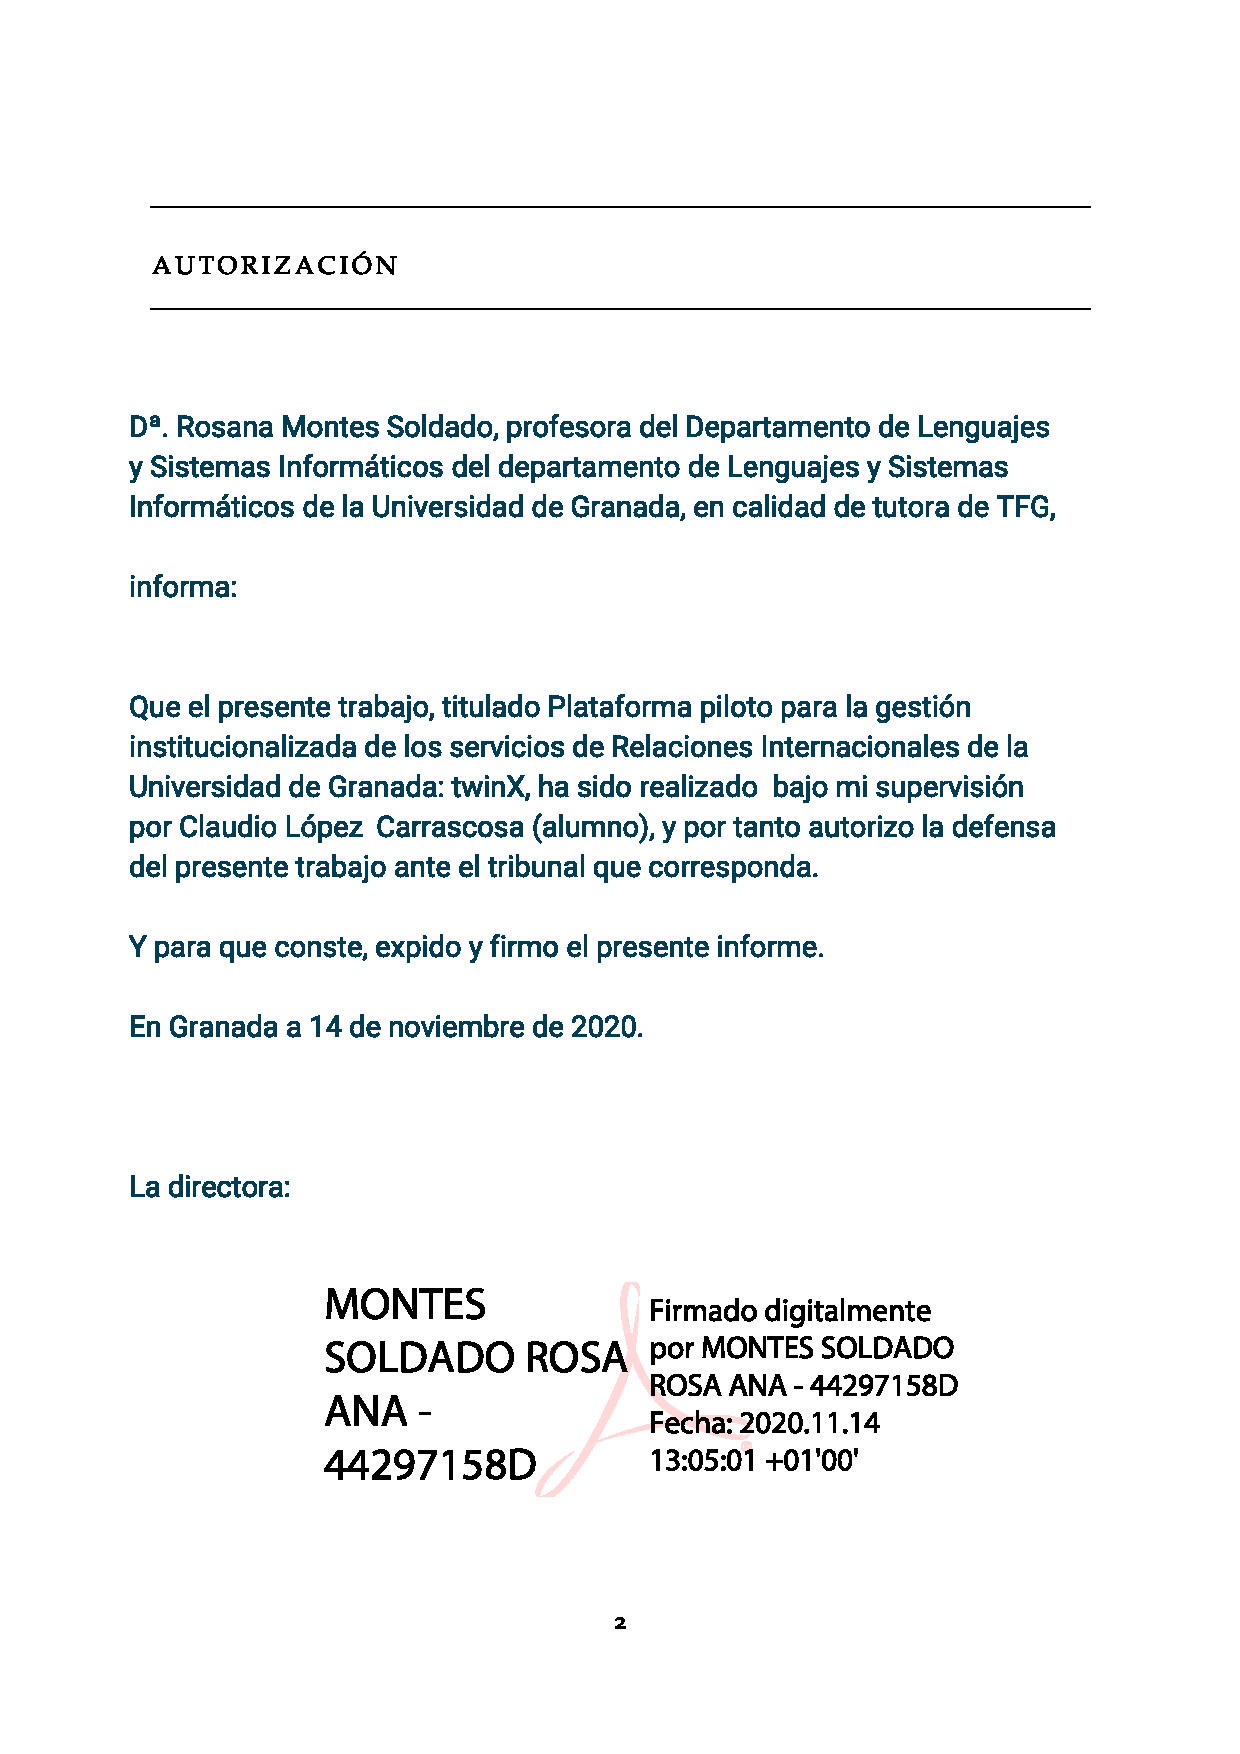
\includepdf{pdf/autorizacion}
\newpage
\chapter*{Agradecimientos}

Hoy termino lo que comencé hace aproximadamente cuatro años. Siempre tuve más o menos claro que la informática era lo mío. Todo comenzó cuando mi padre me inició en el mundo de los ordenadores montándome mi primer equipo cuando tenía cerca de seis años. Mi madre nos oía extrañada --y lo sigue haciendo-- cuando hablábamos de asuntos que se salían de su entendimiento. Es cierto que ninguno de ellos me ha enseñado conceptos muy avanzados sobre informática, pero cuando uno llega al fin de una etapa como esta se da cuenta de que hay muchas más cosas como la actitud, el respeto y el ser buena persona que influyen como lo que más y son las herramientas más valiosas. Y en eso han sido mis principales maestros, pues si hoy soy quien soy, no es más que gracias a ellos y a su constante esfuerzo por que mejore como persona día a día. 

Ellos me hicieron el regalo de traer a mi hermana al mundo, quien también me ha enseñado lecciones tan importantes como las de mis padres, y a la que quiero con toda mi alma por endulzar mi vida y hacerme crecer aún más como persona. Somos muy distintos en lo externo, pero en lo interno ambos sabemos que somos como dos gotas de agua.

No, la familia no se escoge, pero si tuviera que hacerlo os volvería a escoger a vosotros mil veces más. Gracias, gracias y gracias.

Junto a mí estos cuatro años también han estado mis amigas Beatriz y Mercedes. Por acompañarme, me hicieron hasta una visita durante mi estancia en el extranjero, y es que no son otra cosa que mis compañeras de viaje en la vida. Me han apoyado como nadie y han estado ahí en las tardes de estudio, en los momentos más buenos y en los no tan buenos también. No concibo la vida sin ellas, y por ello les debo mucho. Gracias, hermanas.

Al llegar a Granada me encontré con quien sin saberlo se ha convertido en otro pilar importante en mi vida académica y ya cotidiana: mi compañero de piso Diego García. Unos años después, la ETSIIT me descubrió a Diego Cortés. Hoy día sigo compartiendo hogar con ellos, quienes también han estado al pie del cañón para escucharme cuando lo necesitaba y para compartir vivencias juntos. Os quiero.

A mis abuelos, que siempre me preguntan por los estudios y siempre velan por mi seguridad y bienestar.

A mis amigos de clase, con los que tampoco habría sido nada igual: Ceci, Carlos, Nabil, Rafa, Pablo, Dani. Gracias por hacer mis tardes en la escuela mucho más amenas, por darme tantos buenos momentos y por haberme acogido con vosotros tan deprisa. Sois de lo mejor que me llevo.

A mi tutora Rosana, por confiar en mí para la realización de este proyecto y por apoyarme para sacar adelante mi propio tema cuando tenía dudas sobre su viabilidad. Sin tu empujón probablemente no lo hubiera disfrutado tanto como lo he hecho.

Incluso a todos aquellos que me reconocen como «el delegado», mis compañeros de promoción de segundo. Gracias por vuestra admiración, el reconocimiento y la gratitud es siempre lo que me mantiene en pie.

A profesores como Olga Pons, Jesús García, Segio Alonso, Carlos Cano, Ana Anaya: de ellos, aparte de los conceptos, me llevo vuestro entusiasmo por la docencia. Espero que en el resto de sus carreras se encuentren con muchos más estudiantes con sed de aprendizaje. Les deseo lo mejor.

A demás familiares, amigos y allegados que han confiado en mí y en mi valía.

Y a ti, lector, por tu interés en leer mi trabajo.

A todos vosotros,

Gracias.

De corazón.



\newpage
\chapter*{Plataforma piloto para la gestión institucionalizada de los servicios de Relaciones Internacionales de la Universidad de Granada: twinX}

\textbf{Palabras clave:} \textit{relaciones internacionales, internacionalización, UGR, Yii2, web, MVC, sistema de información.}

\section*{Resumen}

\noindent El objetivo de este trabajo es la proposición del proyecto piloto para una plataforma integral de gestión de la internacionalización en la Universidad de Granada. Para ello, se parte de una herramienta con grandes carencias ya creada y se lleva a análisis para poder examinar a fondo las necesidades y así lograr uno de los principales objetivos de este proyecto: dar el salto a la web. Todo ello se lleva a cabo partiendo de la aplicación de metodologías ágiles y enfocadas en el usuario, que tienen como resultado producir un software de calidad y orientado al cumplimiento de las necesidades de los usuarios en su totalidad, que aportan su retroalimentación a lo largo del proceso.
\newpage
\chapter*{Experimental platform for international relations institutionalised management at Universidad de Granada: twinX}


\textbf{Keywords:} \textit{international relations, internationalisation, UGR, Yii2, web, MVC, information system.}

\section*{Resumen}

\noindent This work's purpose is based on the proposal for an experimental project of an integral-solution platform for the internationalisation management at Universidad de Granada. To accomplish it, we start with the analysis of an existent tool with big shortages, so that we can examine in depth its needs and thus achieve one of the main goals of this project: taking the leap to the Internet. Everything is carried through by the application of agile methodologies user-focused methodologies, which have as a result a valuable software production, which aims the fulfillment of the user needs above all, who contribute with their feedback throughout all the process.
\newpage

\setcounter{tocdepth}{4}
\setcounter{secnumdepth}{4}
\tableofcontents


\newpage

\listoffigures
\listoftables

\newpage

% 1. Introducción

\chapter{Introducción}

Desde hace muchos años, las herramientas que hay para gestionar la información en oficinas y secretarías no son --por suerte-- las mismas que antes. Y es que, por pequeña que sea la cantidad de información a manejar, hay cada día más y más formas de hacer las cosas mejor y teniendo en cuenta detalles y elementos que intervienen en la actualización haciendo, por lo general, el proceso más efectivo, eficiente y seguro.

Con este trabajo pretendemos dar un empujón a una solución que fue creada para hacer gestiones, pues estas han ido poco a poco tomando forma de problema. Cada vez hay más información que almacenar, se tiene que disponer de la misma de manera más efectiva y, en general, las exigencias van elevándose conforme pasa el tiempo. Por ello, con este trabajo, vamos a proponer una alternativa a modo de punto de partida, no solo para un ámbito en concreto, sino para muchas otras situaciones en que se tengan preámbulos parecidos al que describiremos. 

\section{Motivación}

La Facultad de Filosofía y Letras es, con 14 enseñanzas de grado y 2000 asignaturas, una de las facultades con mayor volumen de información de la Universidad de Granada. En el curso 2018/2019 se encuentra en cuarto lugar en cantidad de estudiantes con un total de 4733 \cite{MemAcademica}. Es más, se tiene un registro de unos 517 estudiantes entrantes y otros 236 salientes hacia y desde España, haciendo algún programa de movilidad durante el curso 2019/2020 en dicha facultad \cite{MemFYL}.

Resulta obvio pensar en que la relación del tamaño de una entidad con la cantidad de datos que maneja es directamente proporcional. Centrándonos en los datos relacionados a todos los estudiantes que realizan algún programa de movilidad, sería impensable hoy en día manejar semejante cantidad de información sin la ayuda de alguna herramienta que nos permitiera conocer el estado de los mismos (tanto los que vienen del extranjero como los que van a otro país). No obstante, lo cierto es que hasta hace tan solo unos años, desde la Coordinación de Movilidad de la facultad comenzaron con el tratamiento de los datos mediante anotaciones de todo tipo y en cualquier lugar que pudiera parecer seguro y de la forma más organizada posible (si cabía): desde documentos físicos hasta digitales, haciendo casi imposible la realización de numerosas tareas como son la clasificación, búsqueda y selección de estos datos.

Por ello, trataron de aproximarse a lo que comúnmente se utiliza en estos casos: un sistema de información. Hoy en día disponen de una herramienta que si bien les ha hecho reducir el tiempo de trabajo de semanas a unas pocas horas, sigue teniendo muchas limitaciones que no permiten adaptar la forma natural de interaccionar con la información y, por tanto, con el sistema que la alberga de manera total, poniendo en riesgo la consistencia de los datos, su seguridad y su accesibilidad, dificultando al mismo tiempo su integridad y su distribución.

Así, nace la idea de \textbf{twinX}. Se trata de una propuesta cuyo objetivo es, en cierto modo, replicar la funcionalidad de la herramienta actual creada para la Oficina de Relaciones Internacionales de la Facultad de Filosofía y Letras (ORI-FyL), conocida como \textbf{TWINS}. Será necesario establecer una serie de propuestas de rediseño (a nivel interno y al de la interfaz de usuario), un cambio de plataforma a la web y la ampliación de su alcance a la totalidad (o la mayoría) de usuarios que interaccionan con el sistema, entre otras cosas.

\section{Alcance}

La necesidad de una herramienta como la que ya ha sido creada para albergar la información en la actualidad no es una novedad. Son numerosas las facultades que tienen el mismo problema (aunque quizás no al mismo nivel de dificultad, pues posiblemente manejen una menor cantidad de datos), pero es desde luego una labor que no puede llevarse a cabo con directorios, archivos y demás elementos que complican mucho esta serie de tareas para cualquier cantidad de datos, teniendo en cuenta que el tratamiento que se da a veces no es simple, ni mucho menos.

Son varias las facultades que han mostrado interés por implementar TWINS. La Facultad de Ciencias Políticas trabaja en la actualidad con la herramienta y las facultades de Ciencias Económicas y Empresariales y de Bellas Artes están en ello también. En sus comienzos, la importación de datos era algo bastante tedioso y que llevó tiempo para su adaptación. Sin embargo, poco a poco, han notado una gran mejoría respecto a su anterior ritmo de trabajo.

No obstante, twinX no tiene un objetivo tan cerrado a nivel institucional. Se pretende hacer llegar una solución para la gestión de la mayor parte de la información referente a los procesos de movilidad a toda la Universidad de Granada, estableciendo las menores limitaciones posibles, de modo que pueda incluso llegar a usarse en otras universidades que no dispongan de los medios suficientes para organizar y disponer la información tal y como se espera hacer con la herramienta que proponemos.

Es más, algo que dota de atractivo a twinX es acercar la interacción con los datos a la mayor cantidad de usuarios posible que forman parte de los procesos de movilidad estudiantil, lo que presenta probablemente una alternativa muy razonable a las posibles soluciones que las distintas facultades de otras universidades puedan poseer para llevar a cabo sus gestiones en el mismo ámbito.

\section{Objetivos generales}

Este proyecto no es otra cosa que un camino hacia la posibilidad de transportar las gestiones que actualmente están teniendo lugar a una plataforma web.

Se trata de dejar atrás una aplicación enlazada a una base de datos local, todo ello realizado con Microsoft Access\textregistered y obtener a cambio una alta disponibilidad, un buen funcionamiento y una mejoría en la forma de gestionar el trabajo; es decir, se pretende llevar el actual TWINS al navegador, para que se pueda facilitar la posibilidad de acceso desde distintos sitios en lugar de tener los datos centralizados en un único archivo que tiene una infinidad de riesgos de ser borrado, modificado por error, corrompido, etc; todo ello, en aras de mejorar la labor de las distintas oficinas de relaciones internacionales de cualquier universidad.

No es más que la intención de mejorar y perfeccionar lo ya existente: poder consultar la información de una manera más rápida y efectiva, con una mayor comprensión de los menús por los que se pasa en el curso de la interacción con la aplicación, simplificar totalmente la vista, hacerla más atractiva y adaptarla a los sistemas web de hoy en día.

Para poder partir de lo que ya se tiene, se habrá de implementar al menos la misma funcionalidad de TWINS casi al completo. Dejando a un lado los procesos que se consideren redundantes o de poca utilidad, se habrá de incluir aquellos que sean de mayor importancia o representen un mayor manejo de los flujos de información con respecto a la totalidad de la aplicación y se incluirán otros o se modificarán los ya existentes para automatizar el intercambio de datos entre los mismos. Entre todos ellos, cabe mencionar:

\begin{itemize}
	\item Gestión de \glspl{Convenio} entre universidades.
	\item \glspl{AE}.
	\item Expedientes\footnote{Con « expedientes » aquí nos referimos más bien a las etapas del estudiante en su proceso de movilidad y no al expediente académico universitario que alberga sus calificaciones.} de los estudiantes y sus datos personales.
	\item Información sobre los \glspl{Tutor} y su gestión con respecto a los acuerdos de estudios.
	\item \gls{AM} para \glspl{Incoming}.
	\item Comunicaciones masivas, tanto al estudiantado como a los \glspl{Socio} (ver: \gls{Nominacion}).
\end{itemize}

Y con ello, los demás procesos derivados de estos siete módulos principales que se basan en la modificación, supresión y creación de la información que intercambiarán los distintos procesos de twinX.

Junto a esto y centrándonos en el día a día de la labor de una secretaría de internacionalización, hay un gran trabajo que hacer en cuanto a los acuerdos de estudios. Durante la confección de los mismos se intercambian muchas versiones de estos documentos entre los tutores académicos y  los estudiantes que planean su movilidad, y es por ello que proponemos junto con twinX una nueva forma de hacer esto. La idea no es otra que permitir que mediante una identificación, tanto por parte del tutor como por la del interesado/a en hacer una movilidad se pueda confeccionar un acuerdo de estudios online, requiriendo los elementos necesarios para dicho fin y pudiendo, de forma mucho más cómoda, intercambiar las versiones.

Con la idea anterior y en aras de reducir el papeleo al menor posible, una parte importante está en los estudiantes que vienen a estudiar a la UGR o estudiantes \textit{incoming}, como también se les conoce. Tienen que hacer saber a la secretaría qué asignaturas desean cursar y, tras ello, esperar la retroalimentación por parte de la oficina, quien determina si existen plazas disponibles para las asignaturas seleccionadas. Todo ello se haría mucho más fácil si los datos de cada uno de los estudiantes no tuvieran que ser importados a la aplicación, sino que ya existieran en ella misma directamente, pudiendo incluso dar indicaciones a los interesados sobre disponibilidad de plazas y derivados. En el mismo ámbito cabe mencionar los demás documentos que han de entregarse para justificar el fin de estancia en un país de destino, la modificación de los acuerdos de estudios o el \gls{Consentimiento}: todo ello se vería reducido a la interacción con la plataforma twinX, ofreciendo a los usuarios una visión general y compacta del curso de los eventos que marcan los procesos de movilidad.

Es más, una de las tareas que más tiempo requiere es la localización de los distintos usuarios que registra TWINS y que se han puesto en contacto con la oficina, de modo que los moderadores que administran la información de los estudiantes tienen que buscar en distintos sitios según sea la naturaleza de la petición que tengan que atender. Por ello, y dado que el correo electrónico -dando por hecho que éste es el medio de comunicación habitual- es un servicio aislado de la aplicación, proponemos una unificación para simplificar no sólo el curso de las operaciones que el usuario tenga que desempeñar, sino  también la consistencia de la información y la visualización de la misma, poniendo ante la vista una perspectiva más genérica aún del estudiante, lo que terminaría haciendo más efectivo el trabajo.


Todo ello ha de estar respaldado por una capacidad de la plataforma de albergar una cierta cantidad de conexiones al mismo tiempo. Si bien es verdad que no se contempla soportar una elevada carga de peticiones simultáneas debido a que los accesos se condensarán al comienzo y al final de un cuatrimestre académico, se ha de tener en cuenta que se ha de servir la plataforma a tantos estudiantes como deseen acceder a la misma.

% 2. Caso de estudio

\chapter{Caso de estudio: Oficina de Relaciones Internacionales de la Facultad de Filosofía y Letras de la Universidad de Granada}

Para poder realizar un trabajo efectivo y poder tener en cuenta todas las necesidades, hemos de hacer un análisis previo sobre el caso que nos ocupa. Es por ello por lo que tenemos que comprender cuál es su labor, qué servicios prestan al estudiantado, al profesorado, de qué herramientas disponen, cuáles son sus necesidades y por qué.

\section{Sobre la oficina}
La labor principal de la oficina es encargarse de la gestión de los programas de intercambio y la movilidad de los estudiantes e incluso de profesores. Como no podía ser de otra manera, proporcionan la información necesaria para los interesados en estos programas, tanto de fuera de la UGR como desde universidades extranjeras. Es más, también revisan convenios existentes con éstas y hacen otros nuevos para ofrecer cada vez más alternativas para poder mejorar nuestra formación.

En su día a día, atienden peticiones y dudas de los estudiantes que participan en alguno de los citados programas; es más, se dedican a asesorar y mostrar todas las alternativas de las que disponen cuando se nos presenta alguna situación complicada, de modo que podamos resolverlo de la forma en que más nos beneficie. Trabajan, en definitiva, con el futuro de los estudiantes, pues la movilidad la desarrollamos con el objetivo de complementar nuestra formación, algo fundamental y abrumador al mismo tiempo cuando se cruzan fronteras y se quiere seguir en el camino de la educación en una universidad que no es la de casa.

La oficina se sitúa junto a la secretaría, en la Facultad de Filosofía y Letras de la Universidad de Granada, en el Campus de Cartuja, y en ella trabajan alrededor de cuatro personas. Es, dadas las cifras que se tienen, una gran cantidad de información las que tan sólo unas pocas personas tienen que manejar con una herramienta que ha sido creada sobre la marcha para facilitar su importante labor; un trabajo que no puede parar ni tolera fallos, pues los estudiantes de movilidad son uno de los pilares fundamentales de la institución.

\section{Servicio al estudiantado}
\subsection{Estudiantes salientes o \textit{outgoing}}

En relación con los estudiantes salientes, en la oficina se encargan de coordinar a los tutores académicos, que son quienes revisan los acuerdos de estudios que los candidatos proponen para iniciar su movilidad. Una vez éstos les han dado el visto bueno, en la oficina revisan cada uno de los mismos para asegurarse de que todo está en orden. Una vez iniciada la movilidad puede darse el caso en que los estudiantes deseen hacer alguna modificación a su acuerdo, debido a algún cambio imprevisto o a que alguna asignatura no resultara ser como se esperaba, todo ello en el destino. En ese caso, el proceso sería el mismo: tendrían que volverse a revisar de nuevo los documentos para comprobar que todo está en orden.

También escuchan casos de estudiantes con problemas particulares y que deben ser examinados con detenimiento, para ofrecer la mejor alternativa, ya sea hablando con los coordinadores de los destinos internacionales o arreglando algún dato en los convenios que haya causado algún inconveniente en la movilidad de algún(a) estudiante. De este modo, las futuras movilidades podrán hacerse con una mayor posibilidad de éxito, sobre todo cuando se trate de convenios nuevos. Son múltiples los casos en que se deba necesitar asistencia: una lengua de impartición de las asignaturas distinta a la esperada, un nivel requerido en un idioma que no se había comunicado al estudiante, etc.

Una vez los estudiantes vuelven de su movilidad, se inicia el proceso de reconocimiento de créditos, para el cual se establecen unas correspondencias entre las calificaciones obtenidas en el destino y las que se van a especificar en su expediente en la UGR. Para ello, esta información debe estar reflejada en un documento oficial y que la secretaría pueda aceptar, por lo que en muchos casos el personal tiene que ponerse en contacto con los responsables en el destino y solicitar los certificados que sean precisos. De esta manera, se puede tener la certeza de que es alguien de confianza quien los remite, ya que se ha tomar muy en serio la veracidad de los mismos.

\subsection{Estudiantes entrantes o \textit{incoming}}

En cuanto a los \textit{incoming}, el proceso es distinto. Si bien es verdad que se les atiende para problemas similares a los que los estudiantes salientes podrían tener, este grupo viene a la UGR con un acuerdo de estudios previo ya hecho, de modo que es entonces cuando precisan del visto bueno extra de la Oficina, quien les confirma que las asignaturas a las que quieren acceder según lo que establezcan sus acuerdos de estudios tienen plazas disponibles. Es entonces cuando se podrían matricular de las mismas.

Este proceso es conocido como \gls{AM} en el ámbito de la movilidad y se hace de manera manual según las plazas que establece la facultad para cada asignatura. Es gracias a la ayuda de TWINS que puedan no sólo ver estas asignaciones de una mejor manera, sino que también tienen la posibilidad de generar los horarios para los estudiantes, algo fundamental y que les preocupa mucho cuando vienen a hacer su movilidad a la UGR. Pensemos que el simple hecho de que dos asignaturas tengan lugar en la misma hora supone un cambio inminente. Para ello, los interesados tienen que estudiar cuáles son las alternativas de que disponen, atendiendo al número de plazas restantes en las demás asignaturas, no dejando de lado si la franja horaria en la que se imparte clase es compatible con su horario final.

Como es lógico, tendrán que reportar estos cambios que hagan a sus universidades de destino tal y como éstas establezcan, pues al fin y al cabo el proceso para ellos será el mismo por lo general cuando vuelvan a casa.


\section{Servicios al profesorado (PDI)}

Al igual que los estudiantes, el Personal Docente Investigador tiene posibilidad de participar en programas de movilidad; es decir, hay convenios que contemplan la acogida del profesorado.

Es en la ORI-FyL donde gestionan y registran estos convenios. Una vez hay constancia de ellos, el personal puede solicitar un programa, al igual que los estudiantes; no obstante, es la Oficina de Relaciones Internacionales central quien se encarga de sus gestiones a lo largo de la movilidad. Esto es, no establecen una interacción directa con la oficina de la facultad.

En su caso no tienen un acuerdo de estudios, sino que tienen un acuerdo de movilidad o \textit{mobility agreement}, donde se pone de manifiesto la intención y los objetivos de los interesados con el programa que desean hacer.

%COMPROBAR SI HAY REGISTROS EN TWINS Y ACTUAR EN CONSECUENCIA 


\section{Coordinación con la Oficina de Relaciones Internacionales de la UGR (ORI)}

Todo comienza cuando la ORI envía los datos de las adjudicaciones de las plazas de movilidad a la secretaría de la facultad. Es entonces cuando comienzan los trámites administrativos: se registra a cada estudiante de acuerdo a su destino para comenzar a confeccionar su expediente en base a su acuerdo de estudios, documentos firmados y demás información necesaria. Todo ello tendrá que quedar en conocimiento de la ORI una vez acabe la movilidad.

Establecen una estrecha comunicación también cuando se tratan asuntos económicos en relación a las becas. Con la confirmación de las fechas de llegada al destino y vuelta al origen se hace un contraste con la información presente en el convenio, que es otro acuerdo que los estudiantes se comprometen a cumplir. Se tiene en cuenta si el interesado/a ha realizado la movilidad durante la totalidad del periodo para la cual estaba prevista. De no ser así, la cantidad económica final tendrá que ser distinta a la prefijada para la ayuda a recibir por los estudiantes.

Por tanto, es de gran importancia guardar toda la información referente al proceso, pues al fin y al cabo la ORI tiene que coordinar que los distintos programas se están llevando a cabo sin incidencias, ya que, al fin y al cabo, es otro organismo asegurador del buen funcionamiento de esta alternativa al estudio continuado en la universidad que tanta importancia tiene hoy en día y que cada vez está más en auge.

\section{La base de datos TWINS}

%TWINS alberga actualmente unos 2055 registros de estudiantes desde el curso 2018-2019, incluyendo a algunos de ellos que han manifestado su intención de realizar un programa de movilidad en la Facultad de Filosofía y Letras durante el curso 2020/2021. 

TWINS alberga desde el curso 2018/2019 un volumen de datos que plasmamos en la tabla \ref{tab:estadisticasTWINS}. Al tratarse de una base de datos en la herramienta ofimática Microsoft Access\textregistered, la aplicación consta más bien de una simple capa a modo de interfaz que permite al usuario interactuar con la base de datos. La presentación de los datos se posibilita gracias a la ejecución de consultas preestablecidas (\textit{Query By Example}) que se almacenan y se indica en qué campos ha de mostrarse la información. Cuando se realiza alguna acción que requiera el borrado, inserción o actualización de registros se hace uso de las macros, que son trozos de código que disponen distintos flujos de información entre las tablas implicadas en dicha operación.

\begin{figure}
	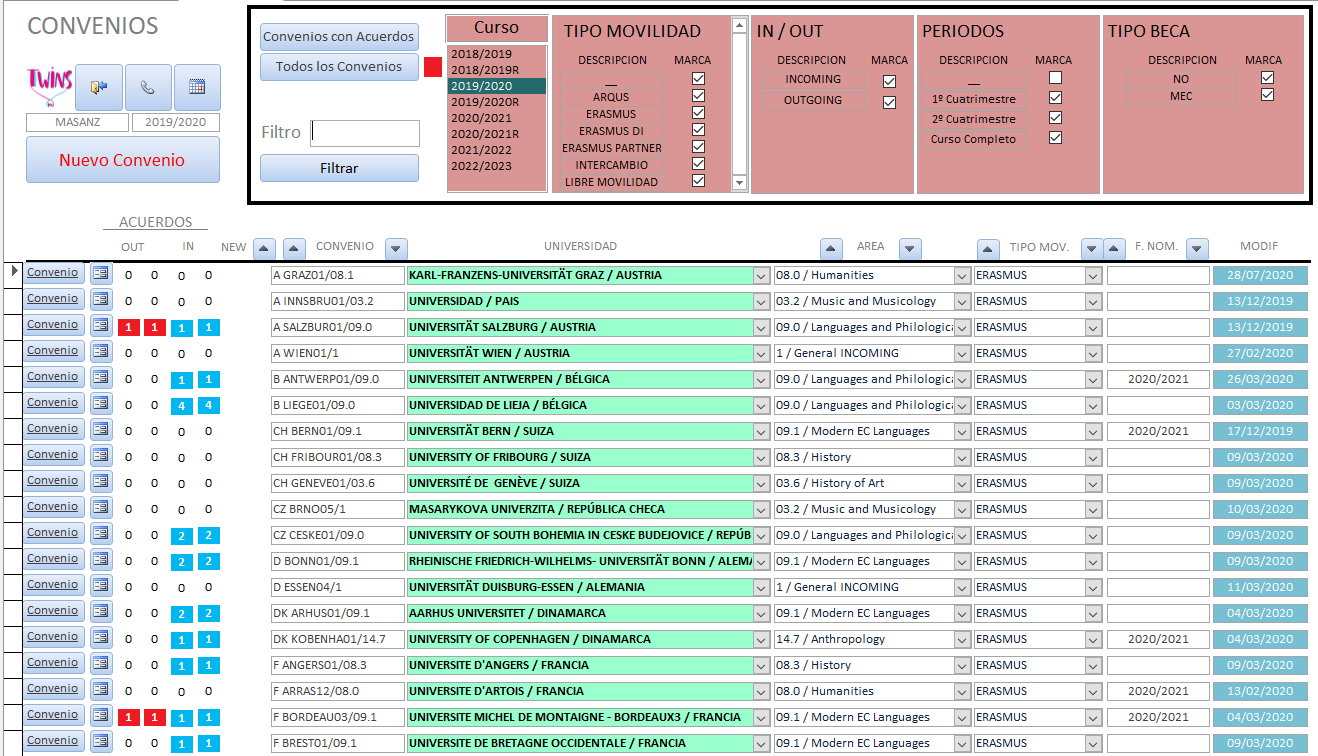
\includegraphics[width=\textwidth]{img/Capturas de TWINS/vistaConvenios.png}
	\caption[Convenios]{Vista de Convenios}
	\label{fig:vistaConvenios}
\end{figure}

\begin{table}[h]
	\begin{center}
		\begin{tabular}{ | c | c | } 
			\hline
			\multicolumn{2}{|c|}{\textbf{Administración}} \\
			\hline
			Estudiantes \footnotemark & 2055 \\ 
			\hline
			Tutores & 58 \\
			\hline
			Convenios  & 607 \\ 
			\hline
			Expedientes & 5049 \\ 
			\hline
			\multicolumn{2}{|c|}{\textbf{Base de datos}} \\
			\hline
			Tablas & 108 \\
			\hline
			Relaciones & 60 \\
			\hline
			Macros & 55 \\
			\hline
			Formularios & 152 \\
			\hline
			Consultas QBE & 343 \\
			\hline
		\end{tabular}
		\caption{Estadísticas de TWINS}
		\label{tab:estadisticasTWINS}
	\end{center}
\end{table}~
\footnotetext{Tanto \textit{incoming} como \textit{outgoing}}



\subsection{El modelo de datos}
\label{ModeloDatos}

El modelo relacional propuesto por Codd es el elegido para el diseño de esta base de datos. Las distintas tablas de la misma se conectan mediante relaciones que establecen restricciones para mantener la consistencia entre los datos.

Las tablas son una forma característica de almacenamiento de este modelo, en contraposición con otras disposiciones de la información usadas por otros sistemas y que, al fin y al cabo, se diseñan de otro modo porque se han de satisfacer unas necesidades distintas.

En este caso, podemos entender que la herramienta TWINS fue creada en Access y, por tanto, en un modelo de datos relacional dado el fácil acceso al usuario no experto en la materia, facilitando la operatividad con las bases de datos.

Es, sin duda, el modelo que más se utiliza aún hoy en día, el cual promete una determinada efectividad siempre y cuando el volumen de información a manejar no sea excesivamente elevado. En este caso, aunque la información que se requiere manipular en la oficina no es fácilmente manejable por personas, sí que aún podemos continuar utilizando este modelo para el desarrollo de la nueva herramienta twinX. Se entiende que no se tendrán más de unos 1000 estudiantes por curso académico (en una sola facultad) y que el número de convenios y tutores no será ni mucho menos parecido, considerando, eso sí, que la cantidad de \glspl{ExpedienteTWINS} será aproximadamente el doble que la de los estudiantes para los que se creen dichos registros.

Así pues, el modelo relacional parecer ser suficiente para las funcionalidades básicas y necesarias para trabajar en la ORI-FyL que twinX pretende implementar.

No obstante, no olvidemos la intención de extender la funcionalidad del actual TWINS para que los propios estudiantes puedan dejar atrás el constante envío de documentos entre sus tutores académicos por correo electrónico, de modo que puedan dar el salto a una plataforma que implemente una interfaz que les permita prescindir de estos documentos, como el acuerdo de estudios, y trabajar con la información directamente (aunque se posibiliten las conversiones a certificados que puedan ser impresos). En este contexto, se ha de tener en cuenta la forma de tratar los datos que se quiere realizar, que tendrá que adaptarse a este modelo de datos que va a ser usado también en twinX.

%Si todas las asignaturas de la universidad de origen se tienen en memoria y tan sólo se tienen que registrar las de la universidad de destino, tan sólo tendríamos que guardar códigos, órdenes y los nuevos nombres para esas asignaturas. Sin embargo, si esto se complicara y tuviéramos que almacenar documentos, quizás, para esa parte de la aplicación, sería conveniente estudiar la posibilidad de implementar una base de datos cuyo modelo de datos esté enfocado a la búsqueda de estos y, no menos importante, optimizado para dicho propósito, algo que sería impensable en una base de datos relacional. Un ejemplo de estas bases de datos es \textbf{Elasticsearch}, que permite hacer búsquedas complejas en texto, a través de datos estructurados y desestructurados. Esta podría ser una buena opción a utilizar una vez se alcance una determinada complejidad en el sistema de almacenamiento, pero en nuestro caso, solo lo comentamos como posibles trabajos futuros.

\subsection{Funciones implementadas}

\begin{itemize}
	\item \textbf{Funcionalidades básicas}\\
	Entre las funciones que hacen que TWINS cobre sentido, destacamos las siguientes:
	
	\begin{itemize}
		\item \textbf{Almacenamiento de información administrativa:} estudiantes, tutores, convenios, expedientes, etc.
		\item \textbf{Asociación de estudiantes con otras entidades:} estudiantes con su tutor, el convenio respecto del cual realizan su movilidad, sus expedientes, etc.
		\item \textbf{\gls{AM}}: para poder organizar a los estudiantes \textit{incoming}
		\item \textbf{Envío masivo de correos electrónicos:} posibilita funciones como las \glspl{Nominacion} automáticas o la comunicación a los participantes en los programas de movilidad de su tutor académico.
		\item \textbf{Generación de documentos automática:} disposición de los distintos datos en documentos que son entregables a estudiantes para mostrarles un sumario de su situación académica
		\item \textbf{Creación, edición y borrado de los datos dentro de la aplicación}
		\item \textbf{Anotación de futuras modificaciones a documentos ajenos a la oficina:} como son, por ejemplo, los convenios, que quedan registrados en la sede de la UGR y no pueden ser modificados hasta una fecha concreta, fuera del control de la ORI-FyL.
		\item \textbf{Recuperación de información de otros formularios externos a la aplicación:} para el registro de nuevos estudiantes (que es hasta ahora la mejor aproximación a la automatización de dicho proceso de la que se dispone) y, por ejemplo, para registrar datos de estudiantes afectados de alguna manera por la COVID-19.
	\end{itemize}

	\item \textbf{Funcionalidades específicas}\\
	Entre las que destacan la generación de informes con fines estadísticos para la oficina, información de asignaturas o menús para gestionar formularios creados por el personal para poder posteriormente transferir la información a la herramienta TWINS.
	
	También disponen de un sistema de alertas en relación con las tareas a realizar por el personal y con una especie de calendario donde se notifican los eventos temporales más próximos a atender.
\end{itemize}

\subsection{La interfaz de usuario}

Como hemos señalado en anteriores secciones, toda la aplicación yace sobre la herramienta de Microsoft\textregistered. Por ello, tanto los datos, como la presentación o vista y el control ejercido sobre los mismos no tiene separación alguna.

Al margen de esto y analizando las ventajas que el uso de Access\textregistered \ nos podría aportar, tenemos una manera de crear una interfaz de usuario de una manera más sencilla de lo normal. Tan sólo basta con arrastrar y redimensionar un botón con el ratón y una casilla para mostrar texto y con unas simples instrucciones tenemos una acción que, al pulsar el nuevo botón, en la casilla podría mostrarse, por ejemplo, cuántos registros almacena una determinada tabla (o varias de ellas) en la base de datos. Las consultas a la base de datos pueden almacenarse y reutilizarse según se quiera. A las interfaces se las conoce como \textbf{formularios} en Access\textregistered

También pueden programarse como si de una consulta se tratara, acciones que impliquen la modificación, borrado o creación de registros en la base de datos. A estas piezas de código funcionales se les da el nombre de \textit{macros}.

Una vez mencionadas las posibilidades funcionales, abordemos el uso de las mismas que han hecho para construir TWINS.

Lo primero que nos encontramos tras abrir la aplicación, es una pantalla de login con los distintos usuarios que pueden acceder al sistema (figura \ref{fig:login})

\begin{figure}
	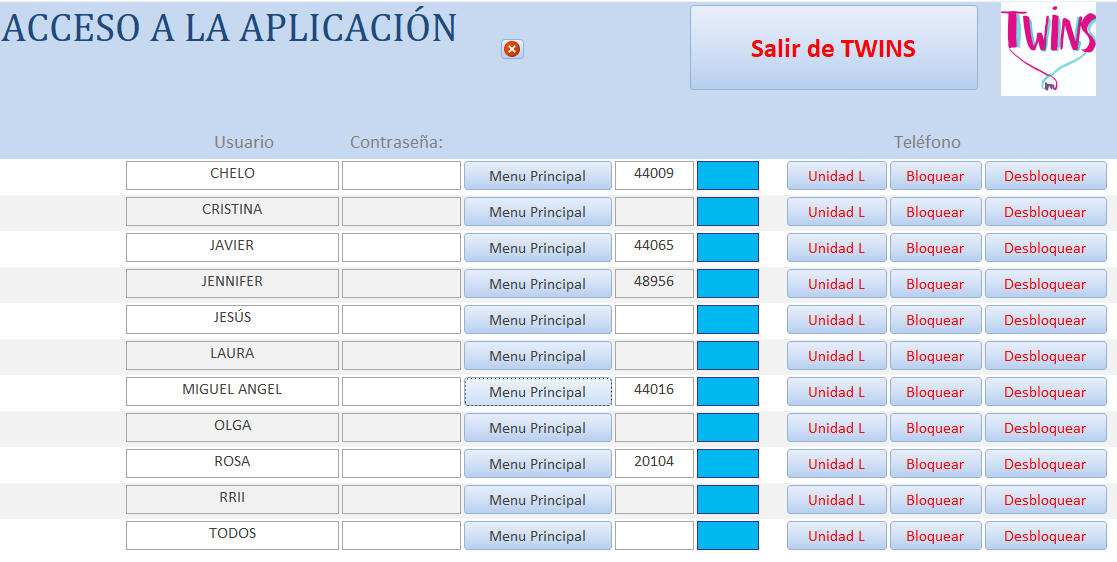
\includegraphics[width=\textwidth]{img/Capturas de TWINS/login.png}
	\caption[Login de TWINS]{Vista del login inicial de TWINS con todos los usuarios}
	\label{fig:login}
\end{figure}


Tras identificarnos, nos topamos, antes de llegar a la pantalla principal, con tres pantallas más:

\begin{itemize}
	\item El calendario (figura \ref{fig:calendario}) proporciona una vista genérica de todos los eventos que tienen lugar y que conciernen a la ORI-FyL o que tratan de asuntos relacionados con la misma. También se guardan plazos para realizar determinadas tareas. Los eventos del calendario\footnote{Nótese la especificación de «evento de calendario» o «\gls{EventoExpedienteTWINS}» en las definiciones correspondientes para establecer la diferenciación entre eventos que tienen que ver con la planificación en el calendario y los que componen los \glspl{ExpedienteTWINS}} son públicos a todos los usuarios de TWINS y en la creación de las entradas en él se permite establecer un(a) encargado/a de la tarea (figura \ref{fig:nuevatarea}), de modo que de un vistazo puedan verse los avisos pendientes que se tienen para un determinado evento.
	
	\begin{figure}
		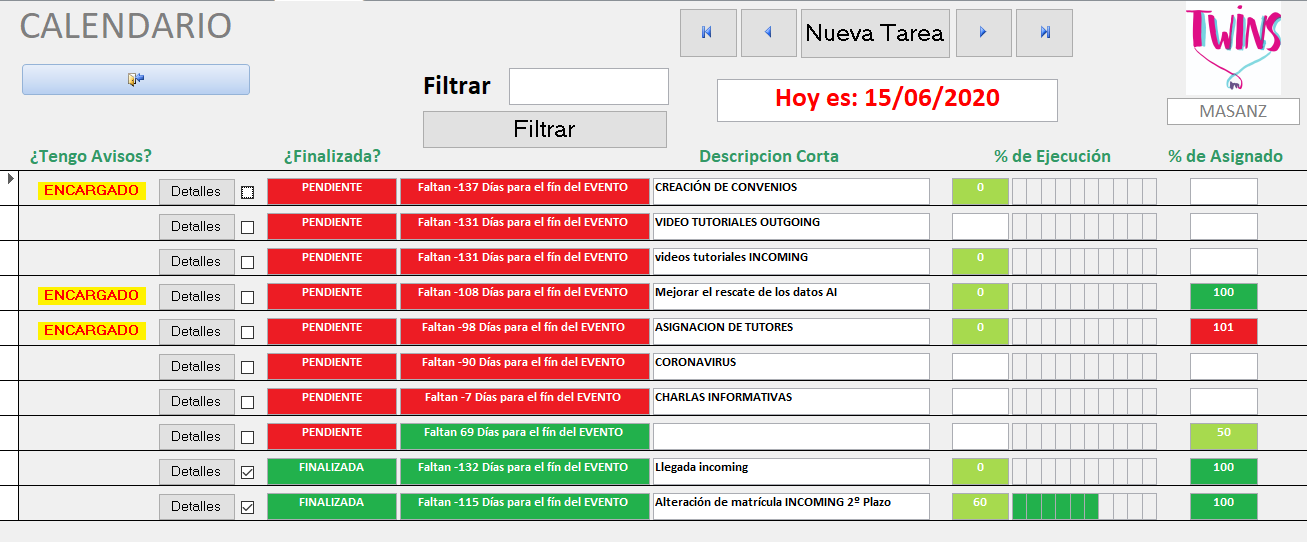
\includegraphics[width=\textwidth]{img/Capturas de TWINS/calendario.png}
		\caption[Calendario de TWINS]{Vista del calendario en TWINS con los eventos existentes y visibles por todos los usuarios}
		\label{fig:calendario}
	\end{figure}

\begin{figure}
	\centering
	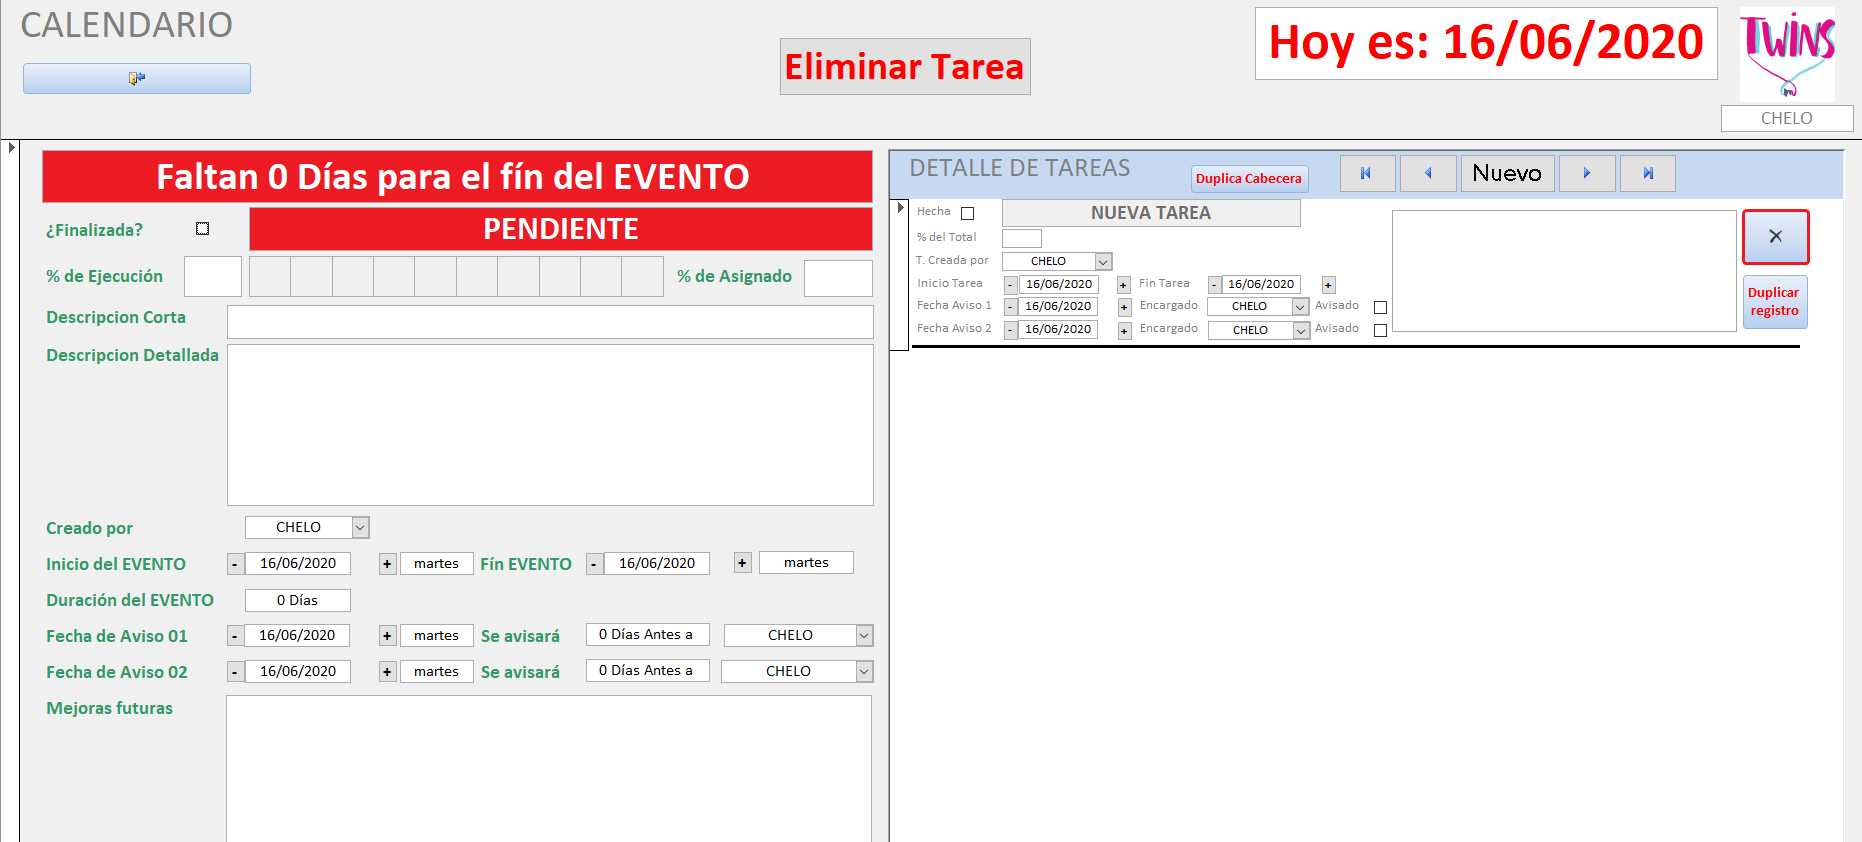
\includegraphics[width=\linewidth]{img/Capturas de TWINS/nuevaTarea}
	\caption[Creación de un nuevo evento en TWINS]{Creación de un nuevo evento en TWINS con la posibilidad de asignar tareas a otros usuarios}
	\label{fig:nuevatarea}
\end{figure}

	
	
	\item La pantalla de avisos (figura \ref{fig:avisos}) nos alerta de las acciones que tenemos que realizar con mayor urgencia, dado que han sido programadas para tenerlas listas para una fecha cercana y necesitan de la atención del usuario al que se notifica. Los avisos, al igual que un mensaje cualquiera, tienen emisor y receptor; es decir, hay alguien que los crea y los dirige a otra persona. Cuando se añade un evento al calendario, se especifican ambos actores, de modo que cuando está próxima la fecha de alguna tarea, se crea el aviso y notifica a aquel al cual le ha sido asignada. Normalmente, un usuario solo puede visualizar los avisos que le han sido dirigidos, salvo el administrador, quien puede ver todos los avisos de todos los usuarios aparte de los propios
	
	Por supuesto, también se pueden crear avisos fuera del contexto de los eventos de calendario, lo que también implica la existencia de emisor, receptor y fecha de caducidad. Al margen de la importancia que se le da a la notificación del número restante de días para que una tarea caduque, esta última forma de hacer uso de los avisos podría verse como imaginando al creador, en la oficina, dejando una nota adhesiva en la mesa de su compañero/a.
	
	 \begin{figure}
	 	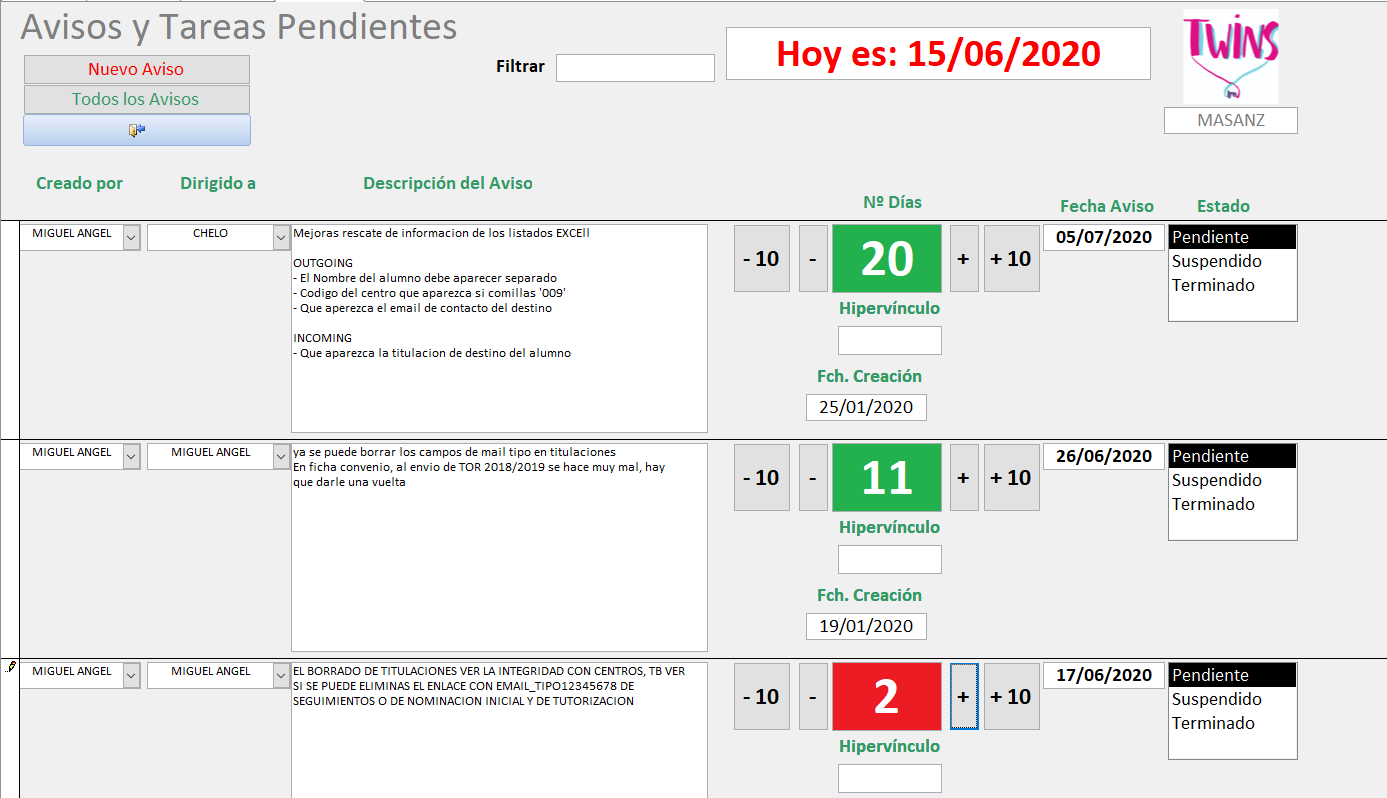
\includegraphics[width=\textwidth]{img/Capturas de TWINS/avisos.png}
	 	\caption[Avisos de TWINS]{Vista de los avisos en TWINS desde el usuario administrador}
	 	\label{fig:avisos}
	 \end{figure}
	 
	
	\item Dejando atrás los plazos y los eventos del calendario, otro elemento de gran importancia y con lo que trabajan día a día en la ORI-FyL (y no sólo en un cierto momento del cuatrimestre académico) son los \glspl{EventoExpedienteTWINS}. Pensemos que a diario surgen problemas, inconvenientes o simplemente hay que actualizar la situación de un estudiante. Por ello, la siguiente pantalla tras descartar las dos anteriores es la de eventos (de expediente) sin procesar (figura \ref{fig:eventosSinProcesar}).
	
	En ella, los usuarios de gestión pueden acceder a la información relacionada con el evento, como los demás eventos, los expedientes del alumno para el cual se está mostrando la información, o directamente las fichas del estudiante o el convenio en sí mismas.
	
	\begin{figure}
		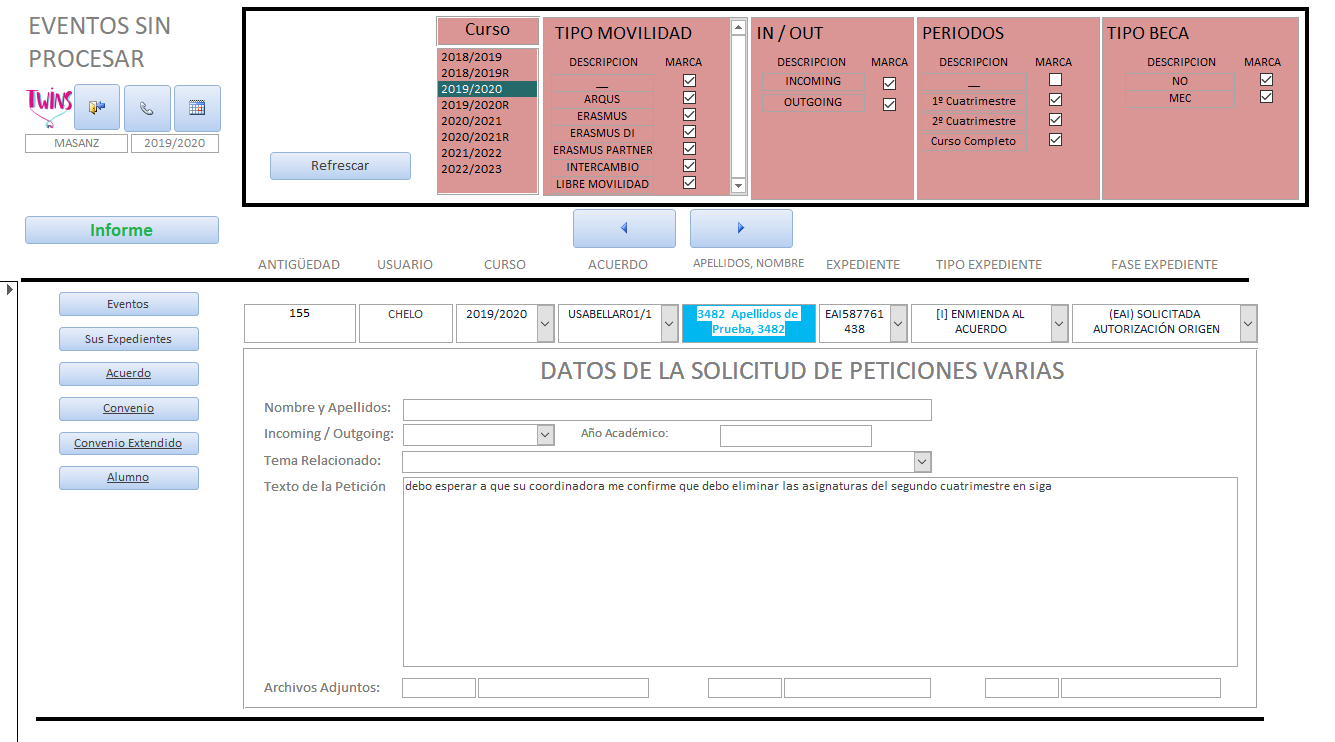
\includegraphics[width=\textwidth]{img/Capturas de TWINS/eventosSinProcesar.png}
		\caption[Eventos sin procesar de TWINS]{Menú de eventos sin procesar en TWINS, una pantalla donde los usuarios ven fácilmente el trabajo acumulado}
		\label{fig:eventosSinProcesar}
	\end{figure}
	
	
\end{itemize}

Finalmente, llegamos a la pantalla principal (figura \ref{fig:pantallaPrincipal}), de donde parten todos los menús (incluso los que acabamos de ver, que se muestran automáticamente identificarse correctamente en el sistema). En ella, no vemos ninguna información como la presentada en capturas anteriores (ni indicador de notificaciones, mensajes o alertas; nada). Lo que sí podemos apreciar es una selección en la cabecera de la vista principal con la que se filtrará el contenido que aparezca tras acceder a cualquier elemento del menú. Esto es, al solicitar determinada información cuando entremos a cierto menú, sólo se nos mostrarán aquellos datos que estén especificados en dicho cuadro de filtrado. Así, las consultas que se pueden hacer a la base de datos son mucho más cómodas y accesibles a todos los usuarios que no tienen por qué tener conocimiento de estos sistemas.

\begin{figure}
	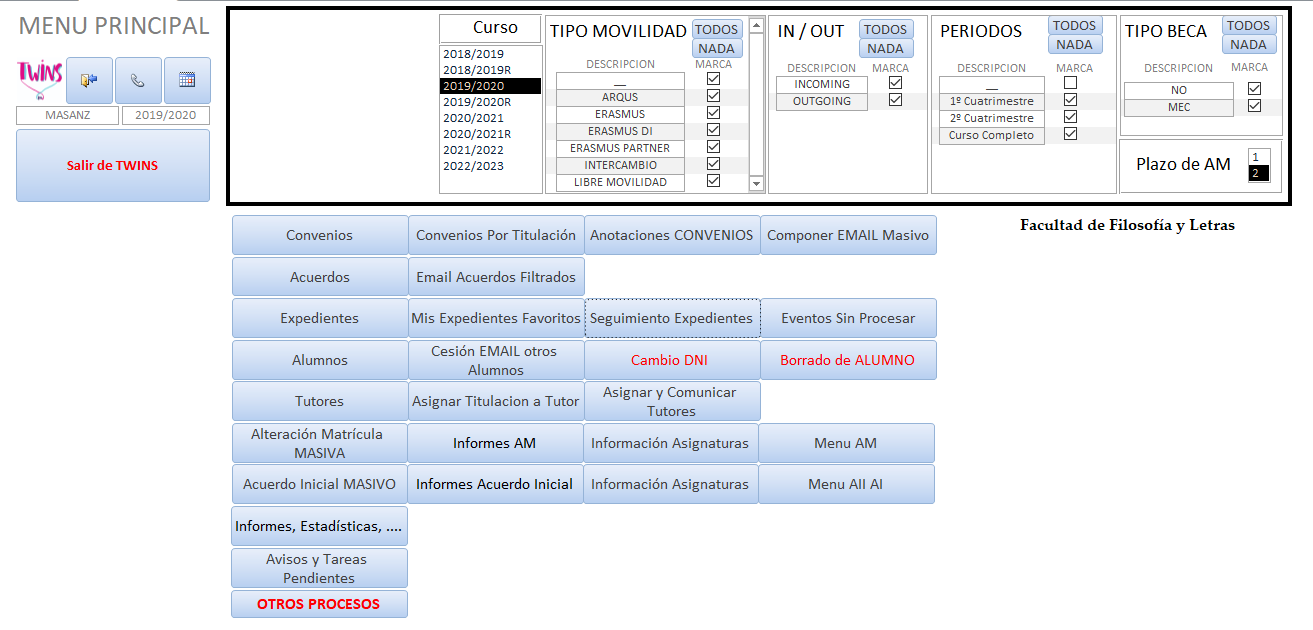
\includegraphics[width=\textwidth]{img/Capturas de TWINS/pantallaPrincipal.png}
	\caption[Menú principal de TWINS]{Pantalla principal de TWINS. Desde aquí podemos acceder a todos los menús anteriormente mostrados.}
	\label{fig:pantallaPrincipal}
\end{figure}

Si accedemos, por ejemplo, a la vista de convenios que ya hemos mostrado con anterioridad (figura \ref{fig:vistaConvenios}), el cuadro de filtrado se nos bloquea (ya hemos hecho una consulta y, para hacer otra, con otros parámetros, tendríamos que retroceder y volver a establecer nuestras preferencias de búsqueda). Se listan los convenios tal y como se han solicitado. El orden puede variarse a través de las flechas en las distintas columnas. Sin embargo y como es lógico, no se muestra toda la información de una tabla. Es más, realmente se están solicitando datos de distintas tablas (figura \ref{fig:tablasConsultaConvenios}). Este es un ejemplo de cómo la herramienta de creación de formularios de Access nos permite disponer la información de una tabla de forma más concisa que mostrando la tabla en crudo.

\begin{figure}
	\centering
	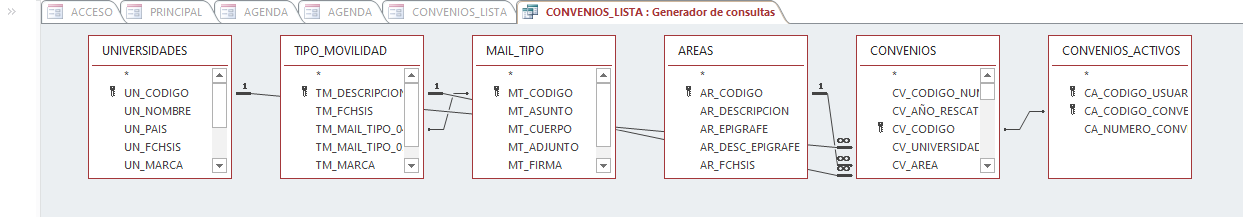
\includegraphics[width=\textwidth]{img/Capturas de TWINS/relacionTablasConsultaConveniosLista.png}
	\caption[Tablas implicadas en consultar convenios en TWINS]{Relación de tablas implicadas en la consulta realizada para listar los convenios en TWINS}
	\label{fig:tablasConsultaConvenios}
\end{figure}

Si nos fijamos en las distintas entradas de la lista en la figura \ref{fig:vistaConvenios} de nuevo, correspondiente cada una a un distinto convenio, vemos que se tienen elementos como un botón para acceder al formulario de la vista del mismo, los estudiantes \textit{outgoing} o \textit{incoming} que están de movilidad según ese convenio, y demás elementos que son de relevancia para la entrada en concreto.

A efectos de diseño de la interfaz, es apreciable que ciertos campos de cada entrada se presentan con un elemento de lista, también conocido como \textit{dropdown}. No son editables hasta que no se accede a la vista del convenio, en contra de lo que puede dar a entender. Si generalizamos al resto de la aplicación, existen numerosos elementos con una disposición extraña como la que mencionamos, de modo que resultan atípicos para el usuario inexperto, lo que podría llevar a confusiones y una pérdida de confianza en el usuario que interactúe con el sistema, a pesar de que no habrá gran cantidad de gente que comience a utilizar el sistema por primera vez de forma avanzada como es la labor del personal de secretaría, quienes sí lo harán. De todos modos, no podemos dar nada por hecho y la labor de un experto en informática es, en esencia, facilitar y mejorar.

Es por ello por lo que gran parte de este proyecto se enfocará al rediseño de la aplicación de TWINS basado en técnicas de usabilidad. Esto será posible gracias a la aplicación de metodologías actuales y la realización de pruebas reales con usuarios que interaccionarán con el sistema.

Para finalizar, vamos a comentar aspectos genéricos sobre las distintas vistas de la interfaz de TWINS. Es un elemento apreciable el uso de colores vivos y que reclaman la atención del usuario. Éstos suelen ser utilizados mayormente en áreas donde se debe prestar mucha atención y se debe proceder con cuidado a la hora de hacer cambios, pues podría desencadenar a un estado de inconsistencia en el sistema difícil de revertir. Ejemplo de esto es el menú de cambio de DNI (figura \ref{fig:cambioDNI}), donde la cabecera es amarilla. La propia aplicación te impide editar el DNI si para el estudiante seleccionado se tienen registros de información. No obstante, no cabe duda de que se trata de un cambio importante, y por eso también, para acceder a dicho menú, hay que hacer doble click en el botón del menú principal (figura \ref{fig:pantallaPrincipal}), ya que sus letras tienen un color rojo, como pasa con cualquier botón que contiene la aplicación y se resalta de esta manera.

También, como elemento en común cada vez que aparece el nombre de los estudiantes, se marca en rojo si es \textit{outgoing} o en azul si, por el contrario, es \textit{incoming}. Ejemplos de esto podemos encontrarlos en las figuras \ref{fig:alumnos} y \ref{fig:cesionDeDatos}. En la primera, podemos también apreciar cómo se presenta un color verde en la columna de casillas más a la izquierda cuando el número de acuerdos de estudios activo para los estudiantes es de 0, lo que significa que «no hay peligro» al editar su información. Si por el contrario tuvieran más de uno, la aplicación mostraría la cifra en amarillo, indicando el alto riesgo de modificar sus datos en caso de hacerlo de forma descuidada. Nótese que no se muestran datos con carácter sensible debido a cuestiones de protección de datos.

Comentemos, en último lugar, que la disposición de estos colores e indicadores no es en vano, no ya a partir de las aclaraciones anteriores, sino también haciendo alusión a la figura \ref{fig:infoAsignaturas}, donde no se tienen datos importantes que modificar, tan solo se trata de una mera consulta --sin derecho a modificación-- a las asignaturas registradas para los estudiantes en la base de datos, no habiendo riesgo de comprometer la consistencia de la información. Es por ello por lo que la paleta de colores, aunque de discutible empleo en toda la aplicación, es muy reducida en esta vista concretamente, pues tan solo se resalta en azul la cabecera, y el resto queda en blanco y negro.


\begin{figure}
	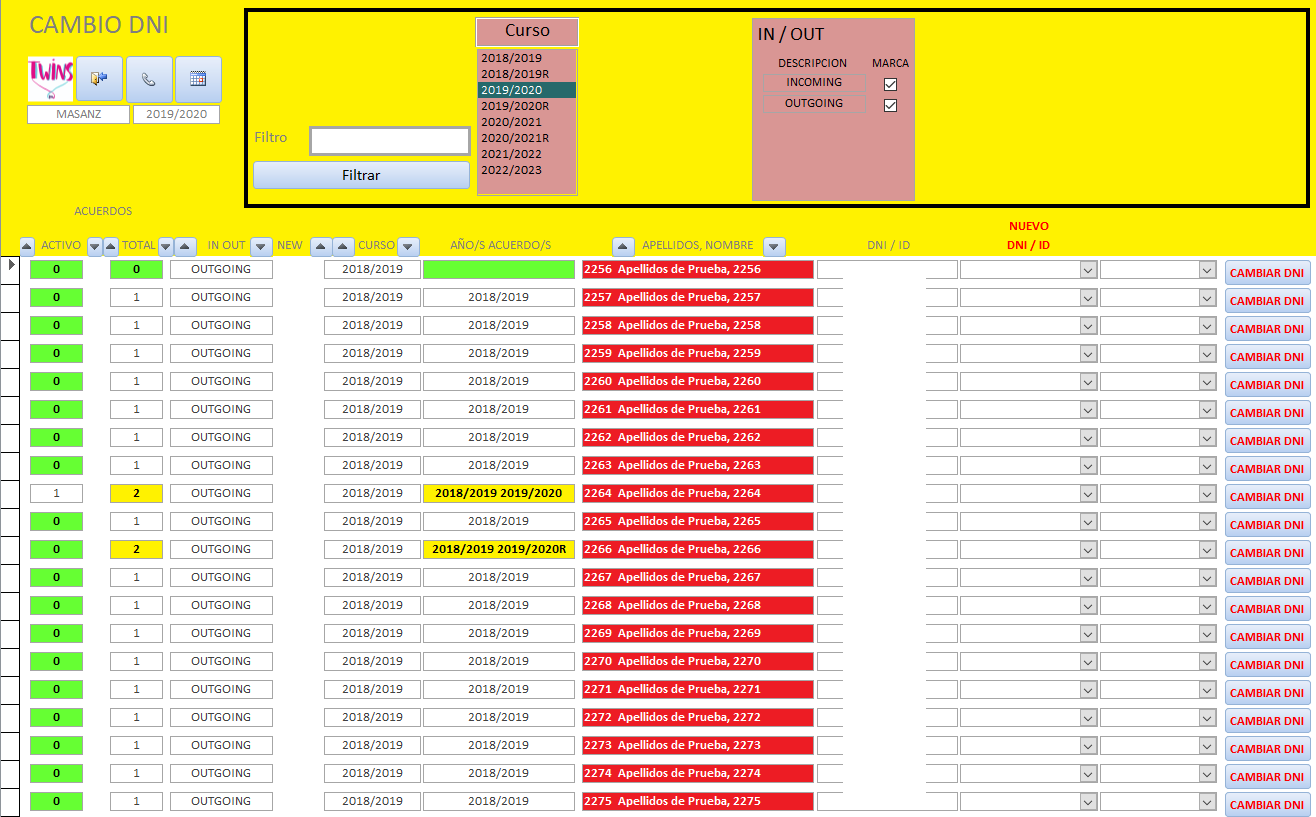
\includegraphics[width=\textwidth]{img/Capturas de TWINS/cambioDNI.png}
	\caption[Menú de cambio de DNI]{También existe en TWINS un menú específico para el cambio de DNI}
	\label{fig:cambioDNI}
\end{figure}

\begin{figure}
	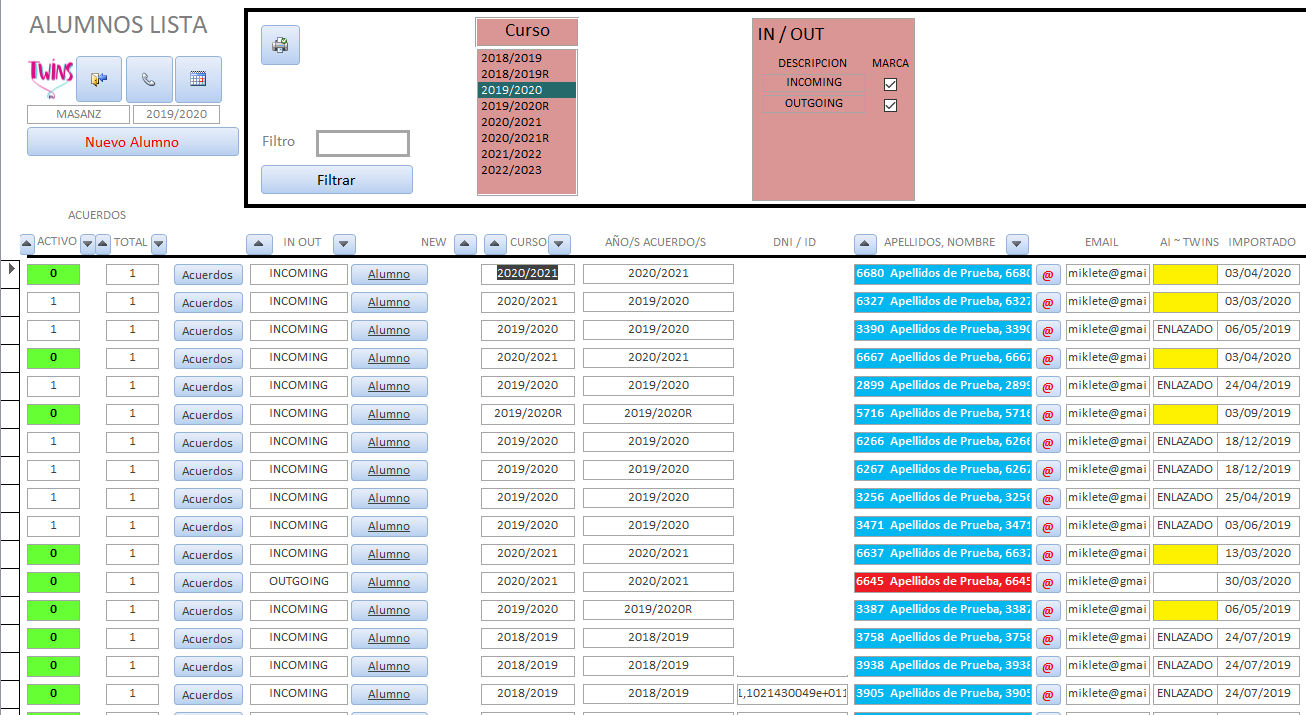
\includegraphics[width=\textwidth]{img/Capturas de TWINS/alumnos.png}
	\caption{Vista de alumnos en TWINS}
	\label{fig:alumnos}
\end{figure}

\begin{figure}
	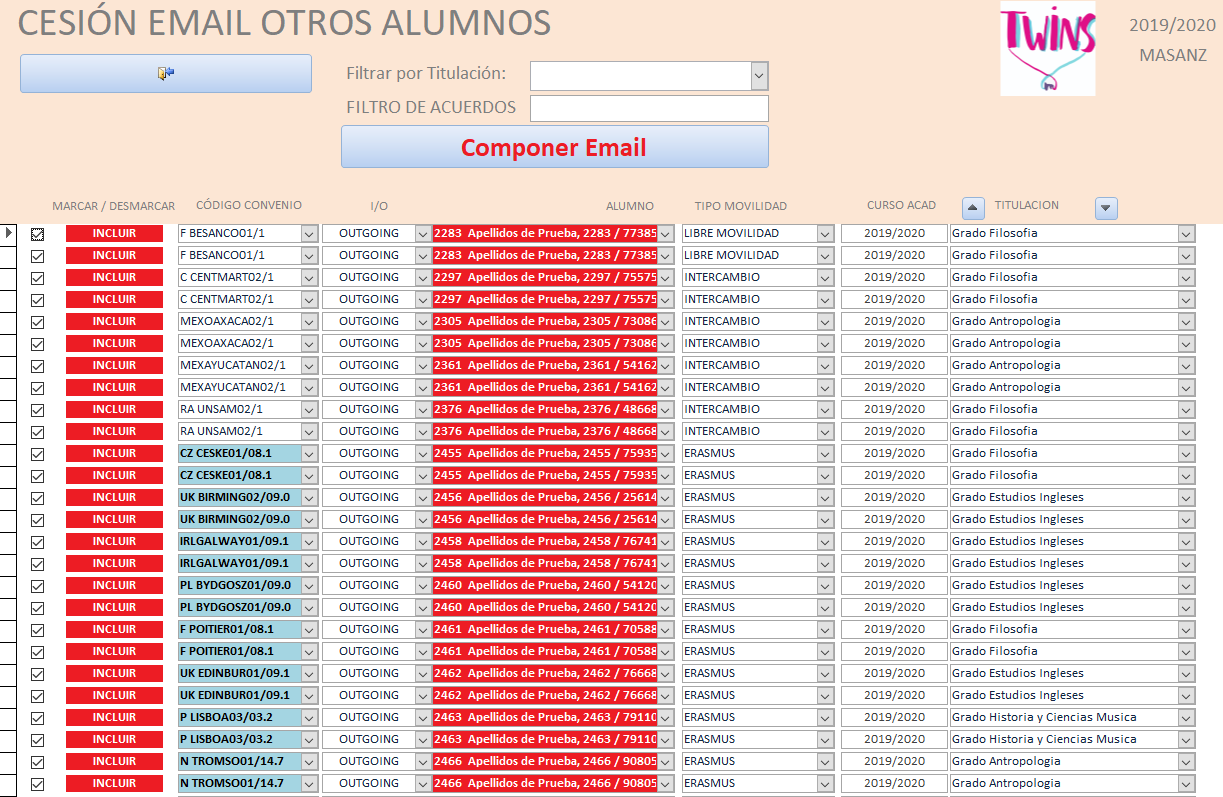
\includegraphics[width=\textwidth]{img/Capturas de TWINS/cesionDeDatos.png}
	\caption[Consentimiento de datos en TWINS]{Menú de gestión del consentimiento de cesión de datos de los estudiantes salientes en TWINS}
	\label{fig:cesionDeDatos}
\end{figure}

\begin{figure}
	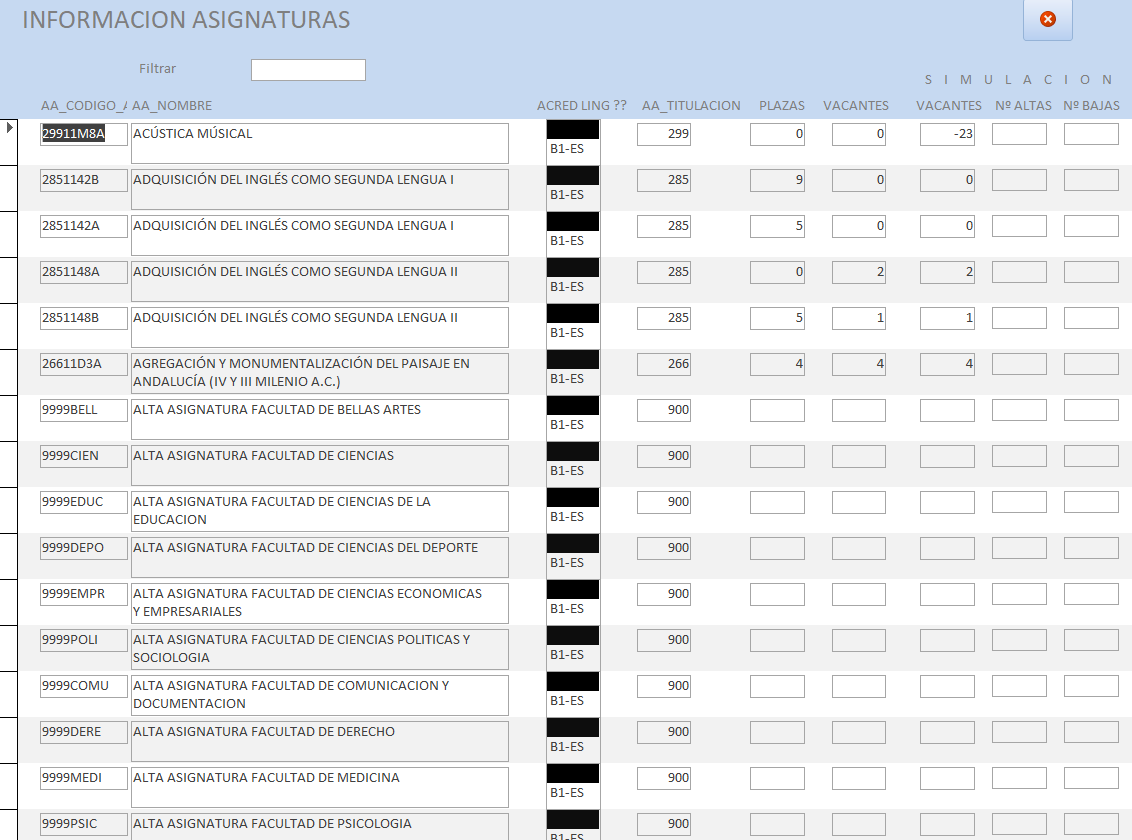
\includegraphics[width=\textwidth]{img/Capturas de TWINS/infoAsignaturas.png}
	\caption[Vista de información de asignaturas en TWINS]{Menú de información de las asignaturas en TWINS (en la universidad local, de destino, de cara a los estudiantes entrantes)}
	\label{fig:infoAsignaturas}
\end{figure}



\section{Estudio de necesidades de la ORI-FyL}

En general, la Oficina de Relaciones Internacionales de la facultad dispone de una herramienta que, dado que ha sido creada por un integrante de la secretaría de la facultad con una estrecha relación laboral con los miembros de la oficina, ha sabido cumplir los requisitos  operacionales del servicio. Muchas funcionalidades de la misma son muy concretas a las necesidades de la ORI-FyL (informes imprimibles con documentación específica, estadísticas, pegatinas para fundas de plástico, etc.)

No obstante, debido a las limitaciones de la metodología escogida para posibilitar estas gestiones, se ha llegado a un punto en que es muy complicado realizar modificaciones y extensiones a la misma. Por ejemplo, la ORI-FyL destaca la necesidad de un portal directamente conectado a la aplicación principal que posibilite la realización de gestiones por parte de los estudiantes. De este modo, tanto el estudiante como el personal de secretaría ahorrarían tiempo y su interacción no sería íntegramente en el correo electrónico. Esto es también extensible al papel de los tutores académicos.

Actualmente se ha hecho uso de herramientas auxiliares como los Formularios de Google\textregistered \ que permiten volcar datos al formato de hoja de cálculo, con lo que permite a TWINS reconocer la información y que pueda, a través de macros, crear nuevos registros en la base de datos para almacenarlos. Sin embargo, se precisa de la interacción humana para dicha tarea, al igual para muchas otras que se puedan querer automatizar o adaptar, como por ejemplo:

\begin{itemize}
	\item \textbf{Adaptar la mensajería} e implementarla dentro de la aplicación para llevar un mejor control de los casos de los estudiantes.
	\item \textbf{Automatización del seguimiento de las nominaciones} teniendo un portal externo donde otras universidades puedan nominar a sus estudiantes en la UGR.
	\item \textbf{Portal con vista para el estudiante entrante}, posibilitando que haga su propio registro en la plataforma y pueda ver su información en ella.
\end{itemize}

Al margen de las nuevas características a incluir, no podemos dejar de lado la necesidad de reconstruir un sistema desde cero, para que sea consistente, estable, con alta disponibilidad y fiabilidad y que pueda adaptarse a las necesidades tanto del personal de la oficina como a las del estudiantado. Es por tanto por lo que debemos descartar seguir utilizando la herramienta de Access\textregistered \ dadas sus limitaciones, expuestas en la sección \ref{ModeloDatos}.

% 3. twinX

\chapter{twinX}

Una vez hemos analizado el material ya existente y desde el que partiremos para la construcción de twinX, vamos a ponernos manos a la obra con su desarrollo. Si bien es cierto que no se parte desde cero en cuanto a requisitos, sí que se va a reconstruir la herramienta desde cero, para poder aportar un gran significado a todos los módulos que vayan a formar parte de twinX y así podamos cohesionarlos de una mejor manera.

\section{Desarrollo de twinX}

Vamos a comenzar estableciendo las ideas principales del proyecto, reafirmando el propósito y viéndolo desde otras perspectivas que, aunque parecen obvias, no siempre se tienen en cuenta. Ello nos permitirá asentar las bases del producto software final y dotarlo de calidad.

\subsection{Diseño centrado en el usuario}

Esta disciplina, conocida también como \textit{User-Centered Design} o UCD, destaca por basar las fases del proceso de diseño estableciendo un enfoque constante en aprender del sujeto que utilizará el producto final. Es decir, para la consecución de los objetivos, es necesario tener una retroalimentación constante por parte del usuario final, que será quien vaya orientando nuestros avances según sea su interacción con lo que vayamos desarrollando.

El proceso dispone de unas fases a seguir, como son:
\begin{itemize}
	\item \textbf{Especificación del contexto de uso:} quiénes usarán el producto, para qué y bajo qué condiciones lo harán.
	\item \textbf{Especificación de requisitos:} identificar los objetivos que tienen que cumplirse para dejar a los usuarios satisfechos.
	\item \textbf{Crear soluciones de diseño:} en distintas etapas, desde un concepto poco definido hasta un diseño completo.
	\item \textbf{Evaluación de los diseños:} a través de las pruebas con los usuarios, de forma ideal.
\end{itemize}

\subsubsection{Pautas de Accesibilidad}

El no atender a causas de accesibilidad sería no aplicar correctamente, de alguna forma, el tipo de diseño escogido para el desarrollo del producto. Cuando se hacen pruebas, el objetivo no es otro que adaptar el producto para que pueda ser bien utilizado por el mayor número de usuarios posible y de la forma satisfactoria para ellos. Es por ello por lo que tenemos que abrir el abanico y contemplar que pueden ser numerosos los usuarios que necesiten adaptaciones para interaccionar correctamente con el contenido web.

Para ello, se propone la utilización de los recursos especificados en \textit{Web Content Accessibility Guidelines} (WCAG) \cite{wcag}. Con ello, podemos hacer que la experiencia en el sitio web pueda ser mínimamente satisfactoria para todo usuario que necesite hacer uso de la misma. En efecto, se deberán emplear una serie de técnicas, especificadas en su web, para que twinX sea adaptable. Entre ellas, destacamos la viabilidad de la interacción con el teclado, un texto descriptivo para las posibles imágenes que se puedan incluir, regular el contraste, etc. Con este proyecto, la intención es alcanzar el nivel AA (segundo más exigente), para que la gran mayoría de personas con necesidades especiales puedan usar la plataforma sin problema alguno.

\subsubsection{Encuesta SUS}

La encuesta SUS o \textit{System Usability Scale} es una de las encuestas que se pueden utilizar para evaluar la usabilidad de una cantidad de productos o servicios.

Sus únicos 10 enunciados es una de las cosas que más atractiva la hacen, puesto que hace que los usuarios la rellenen de manera rápida y fácil. También destaca por ser de denominación común y tener un bajo coste, además de poder corregirse inmediatamente después de terminar la encuesta. Es más, es una encuesta que puede aplicarse a casi cualquier tipo de interfaz de usuario, por lo que es muy versátil. Finalmente, cabe destacar la facilidad de entender los resultados, puesto que vienen dados en forma de una puntuación en el rango de 0 a 100.

Sobre los enunciado de la encuesta, tienen una escala de 1 a 5 cada uno, siendo 1 el indicador de mayor desacuerdo y el 5 el de mayor acuerdo. También se suele aportar unas pequeñas instrucciones a los candidatos a tomar la encuesta, indicando la necesidad de contestar todas las preguntas y de no pensarse mucho la respuesta a las mismas.

Para probar la eficacia de esta herramienta como elemento conductor en la creación de una interfaz de usuario a la hora de hacer pruebas y recibir \textit{feedback}, se hizo un experimento con una escala con adjetivos y no con números. Los resultados del análisis (\cite{sus}) vieron una mayor desviación de los resultados a la hora de expresar un mayor desacuerdo (adjetivos como «horrible» o «peor que lo imaginable» con números más próximos al 1). No obstante, en general, y gracias a análisis como el mencionado, se tiene evidencia que asegura que este tipo de encuestas es una buena herramienta a tener en cuenta a la hora de recibir información acerca de cuán bueno es nuestro diseño para los usuarios.

Por todo ello, esta será una de las herramientas que utilizaremos en las pruebas para constatar que los objetivos del proyecto se cumplen y cuáles pueden ser las conclusiones.

\subsection{\textit{Design Thinking}, DT}

El «Pensamiento de Diseño» o \textit{Design thinking} es una técnica de desarrollo que se centra en el usuario, pudiendo detectar y reaccionar ante cambios repentinos en el entorno de los usuarios y sus comportamientos. El objetivo está, mayormente, en abordar problemas con una pobre definición o que no se conocen a fondo para situar al usuario en el centro de todo y poder así enfocar el problema desde otras perspectivas, de manera que se pueda poner la atención en aquello que resulte de mayor importancia para los usuarios.

\subsubsection{Las fases del DT}

El proceso tiene unas fases no necesariamente secuenciales, de modo que puedan adaptarse lo mejor posible al proyecto, teniendo incluso la posibilidad de ejecutarse al mismo tiempo.

\begin{itemize}
	\item \textbf{Empatizar}, tratar de adoptar un conocimiento lo más empático posible del problema que se pretende resolver. Este es un elemento esencial, pues posibilita a los desarrolladores a descartar sus propias primeras conclusiones --erróneas a menudo-- y a entrar en materia con la realidad del cliente y sus necesidades.
	
	\item \textbf{Definir} las necesidades de los usuarios y sus problemas. Es la fase donde se reúnen y ordenan los elementos obtenidos como resultado de la fase anterior. A partir de entonces, se sintetizan para definir los problemas esenciales que se identifican, los cuales dan pie a la creación de \textit{personas}; esto es, la construcción de perfiles humanos en los cuales centrar el desarrollo.
	
	\item \textbf{Idear} y hacer frente a lo que se da por hecho, creando formas alternativas de ver y tratar el problema con soluciones innovadoras, a partir de lo estudiado en las dos fases anteriores.
	
	\item \textbf{Prototipado} de las soluciones pensadas, una fase experimental cuyo objetivo es el de encontrar la mejor solución para cada uno de los problemas encontrados. Los desarrolladores han de producir una versión de bajo coste del producto para investigar cuál es el resultado de haber llevado las ideas a la práctica.
	
	\item \textbf{Pruebas} con lo obtenido, para analizar si realmente se ha llegado a un buen resultado o, si por el contrario, se ha de retroceder a otra fase para redefinir uno o más problemas.
	
\end{itemize}

Como hemos indicado, las fases no siempre siguen el mismo orden. Hay veces que se toman decisiones como la de saltar de la primera fase de empatía a la penúltima de prototipado, probablemente para aclarar las ideas y poder hacer una mejor definición, a través de la muestra de material al cliente que pueda animarlo a dar una mayor retroalimentación. Del mismo modo, si el prototipado no ha ido bien, se puede volver a la tercera y anterior fase, la de construcción de ideas. Incluso podría darse el caso que haciendo pruebas, los desarrolladores nos demos cuenta de que no se ha llevado a cabo una buena ejecución del proceso y sea preciso volver a la segunda etapa de definición de los problemas. Siempre es mejor ir hacia atrás en lugar de comenzar la casa por el tejado, así que toda maniobra que sea apropiada para una mejor construcción del producto y que lo dote de calidad siempre es bienvenida.


\subsubsection{Herramientas del DT}
\label{herramientasDT}

Hay una serie de actividades o técnicas que nos pueden resultar útiles para llevar a cabo el trabajo de desarrollo con eficacia y que suelen tener éxito. Destacamos las siguientes:

\begin{itemize}
	\item \textbf{Creación de personas:} perfiles ficticios de los distintos usuarios que utilizarán el producto software. Creadas en la fase de definición, no solo se especifica el propósito específico de interacción con el producto a mejorar o la necesidad por que exista el software que se quiere desarrollar. Describimos el contexto del personaje, sus inquietudes y, en definitiva, lo que hay detrás de esa persona en más ámbitos que puedan ayudar a comprender por qué es necesario que se tengan en cuenta ciertas cosas a la hora del desarrollo.
	
	\item \textbf{\textit{Brainstorming}:} también conocida como nube de ideas que radican alrededor de un concepto central. Se trata de escribir conceptos que vengan a la cabeza de los intervinientes en la creación del esquema, sin importar los análisis o el futuro que puedan tener en el proceso. Cualquier cosa que tenga que ver con lo que se está tratando es válida, pues lo que aparentemente resulta absurdo podría en muchos casos resolver parcialmente el problema o ayudar a enfocarlo. Así, cuantas más propuestas, mejor se lleva a cabo este proceso, que tiene lugar en la fase de ideación.
	
	\item \textbf{Prototipado en papel:} la creación de prototipos (en la cuarta fase de prototipado) con un material del que todos disponemos es extremadamente sencilla a la par que útil. Cuando las cosas se plasman en un folio, podemos apreciar matices que no nos venían a la cabeza cuando la idea era tan solo un concepto. Si bien es cierto que depende de las dotes artísticas de la persona que dibuja el prototipo, el hacerlo con papel y lápiz ayuda a volcar la concentración de una manera diferente a como se hace cuando se programa o se diseña con herramientas informáticas.
	
	\item \textbf{Mapas de experiencia de usuario:} también conocidos como \textit{Customer Journey Maps}, sirven para representar la experiencia de un usuario a lo largo del tiempo. En ellos plasmamos la forma en que un diseño cubre o no las necesidades de un usuario utilizando un producto o servicio. Es justo por eso por lo que estos mapas han de ser lo más descriptivos posibles, representando con gran detalle las acciones y subtareas que tiene que desempeñar un usuario al usar el sistema.
	
\end{itemize}

\subsection{Aplicación de las metodologías}

En relación con las fases del DT, podemos diferenciar a través de las cuales ya hemos ido pasando. El comienzo del proyecto vino acompañado de una serie de reuniones que se incluyen en los anexos. En este contexto, la fase de \textbf{empatización} se correspondería con las dos primeras reuniones, donde se establecieron un primer contacto y las bases del proyecto, atendiendo al testimonio de los usuarios reales de TWINS, lo que actualmente se está usando para resolver los problemas a los que se tienen que enfrentar en la ORI-FyL. Es más, en la segunda reunión (~\ref{reunion2}) se habló de algunas características ideales y que está costando implementar en el actual escenario, lo que podríamos englobar dentro de la \textbf{ideación}. Por último, ya en la tercera reunión, se tiene la \textbf{definición} de todos los conceptos necesarios para comprender el funcionamiento de TWINS y de la oficina en general. No obstante, a lo largo de esta sección, vamos a continuar esta fase con la definición de más elementos necesarios para llevar a cabo el desarrollo de twinX.

Con esas tres fases cubiertas, se puede dar comienzo a las otras dos: la de \textbf{prototipado} y \textbf{pruebas}, que serán desarrolladas de forma más extensa en las secciones ~\ref{bocetos} y ~\ref{pruebas}. %PENDIENTE: comprobar referencias, ya que han sido puestas antes de tiempo y añadir posibles futuras reuniones y sesiones de pruebas.

\section{Personas ficticias}

Tal y como hemos comentado en la sección \ref{herramientasDT}, una de las herramientas que nos permiten definir el alcance y las necesidades de la aplicación es la creación de perfiles de personas ficticias, candidatos a utilizar twinX en un futuro. De esta forma, tanto por la parte del desarrollo como por la del interesado en el producto final, pueden no solo hacerse una mejor idea de los objetivos del mismo, sino también justificar su creación.

Vamos a tratar de crear tres personalidades lo más variopintas posibles en aras de enfocarnos más aún en el usuario y dotar de mayor calidad el resultado final, de modo que podamos abarcar por completo el entorno de influencia del problema. (Herramienta: \cite{uxpressia})

\begin{figure}
	\centering
	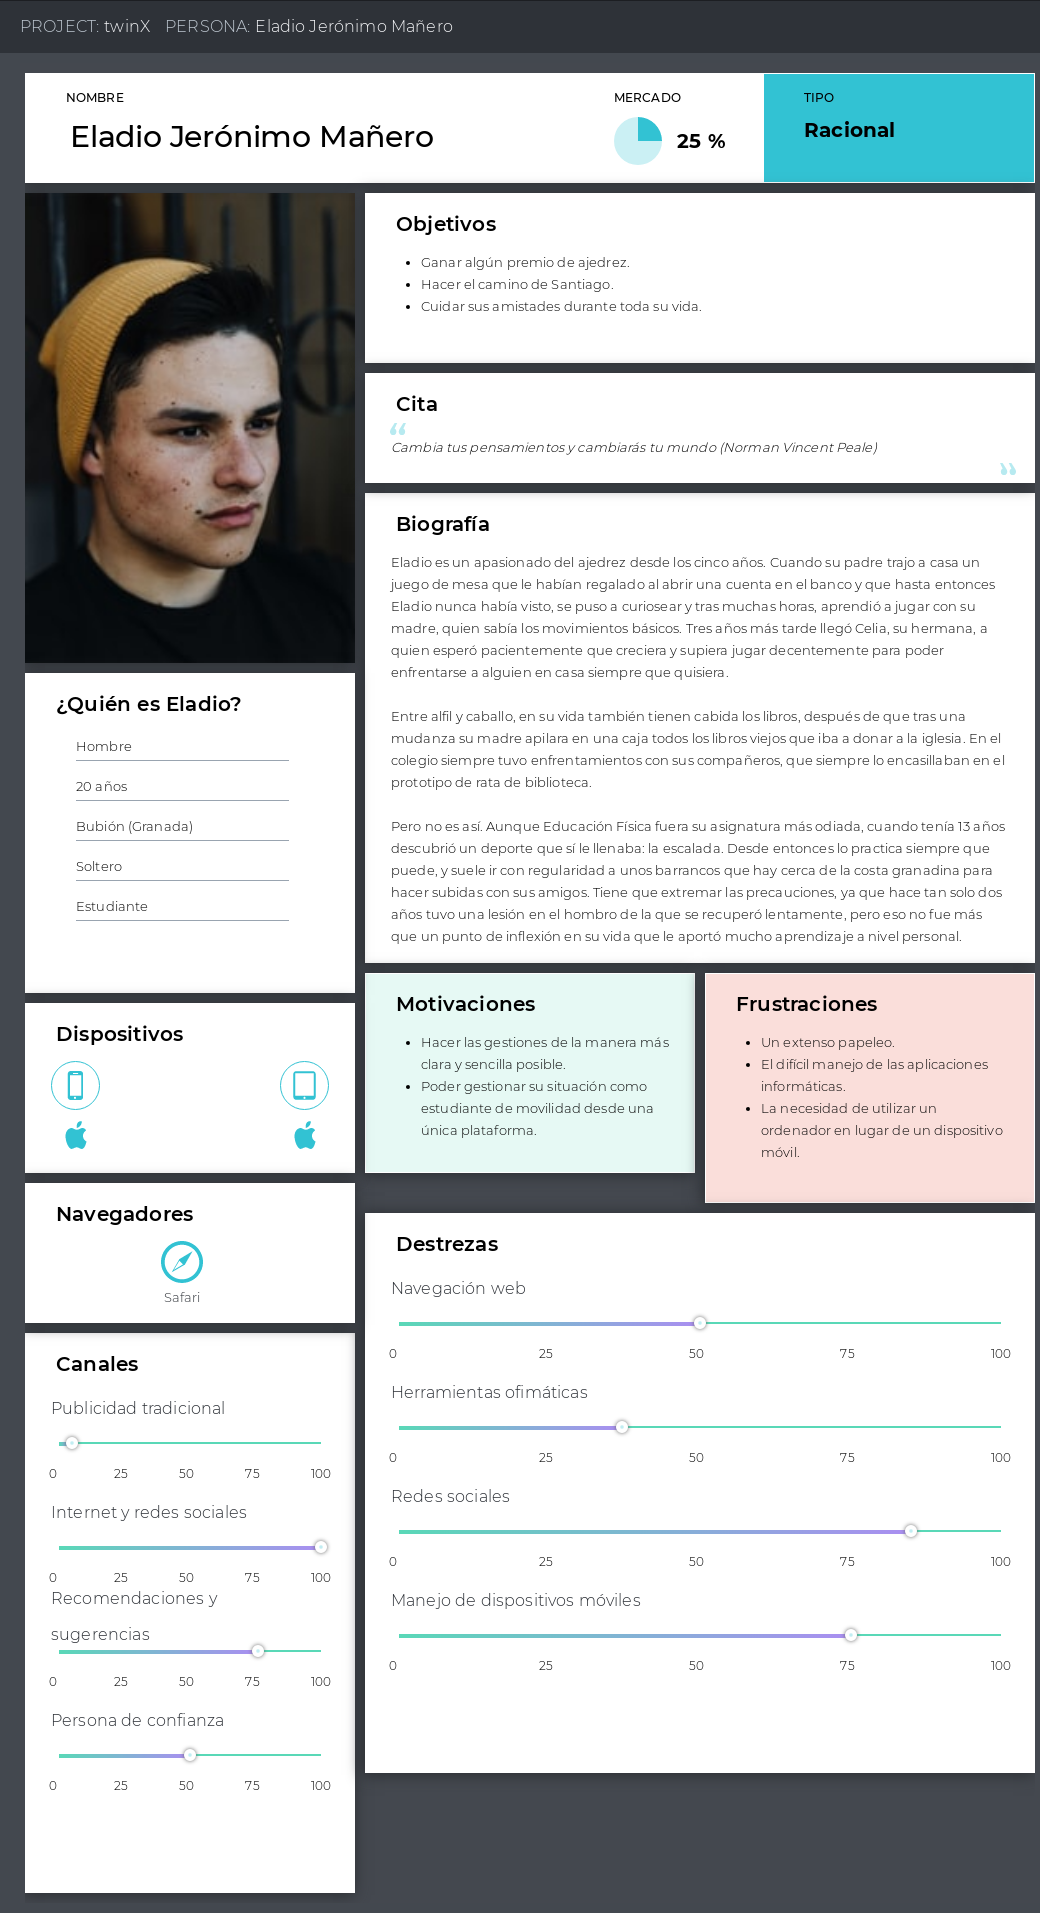
\includegraphics[width=\textwidth, height=\textheight, keepaspectratio]{img/Personas/Eladio}
	\caption[Persona \#1]{Persona \#1: Eladio}
	\label{fig:persona1}
\end{figure}
\begin{figure}
	\centering
	\includegraphics[width=\textwidth, height=\textheight, keepaspectratio]{img/Personas/MGracia}
	\caption[Persona \#2]{Persona \#2: María Gracia}
	\label{fig:persona2}
\end{figure}
\begin{figure}
	\centering
	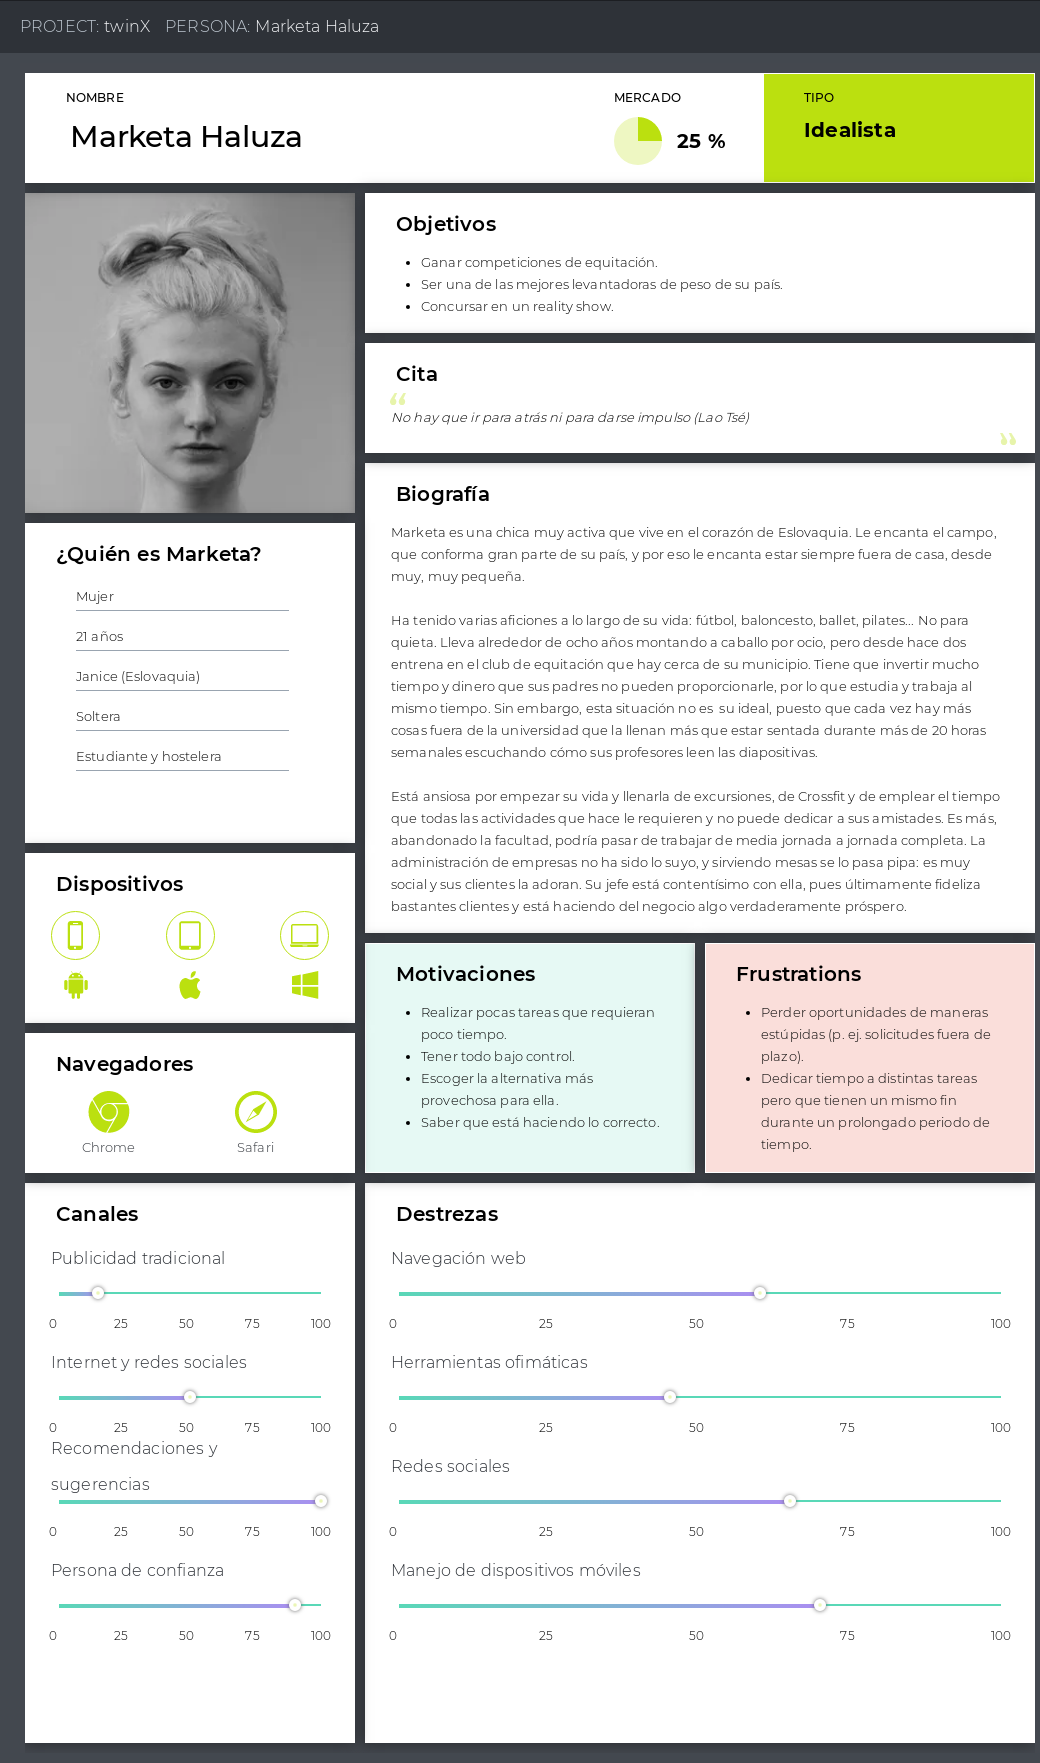
\includegraphics[width=\textwidth, height=\textheight, keepaspectratio]{img/Personas/Marketa}
	\caption[Persona \#3]{Persona \#3: Marketa}
	\label{fig:persona3}
\end{figure}

En vista de la persona en la figura \ref{fig:persona1}, Eladio, podríamos pensar que para él, lo óptimo sería desarrollar una app móvil para poder gestionar su movilidad, en caso de que quisiera hacerla. Pertenece a las nuevas generaciones donde apenas se usa el ordenador, hasta llegar a la universidad, mayormente, por lo que está acostumbrado a una tablet. Al mismo tiempo, María Gracia (figura \ref{fig:persona2}) trabaja gestionando información como la de estudiantes como Eladio o Marketa (figura \ref{fig:persona3}) y no puede permitirse interaccionar con un dispositivo móvil, pues tardaría mucho en realizar su trabajo, y no lo haría de forma efectiva. Por tanto, una solución web parece una resolución del problema apta para la mayoría del mercado del producto.

Como decíamos, nos sirven elementos que no tengan que ver directamente con las habilidades tecnológicas de los candidatos; y es que, por ejemplo, María Gracia en este caso no podría tampoco ver una web que no tuviera la tipografía lo suficientemente grande como para leer, porque podría tener la vista cansada. O quizás Marketa, si no tiene una buena situación económica, tendría quizás que conectarse desde un dispositivo algo obsoleto, por lo que probablemente le sea muy costoso en cuanto a tiempo cargar una página web con numerosas imágenes.

En definitiva, podría pensarse que los perfiles de estas tres personas están hechos para hacer el análisis de cualquier aplicación o producto software, ya que no hemos ideado estas personalidades específicamente para el problema que nos compete. Es por ello por lo que podemos tomar estos perfiles ficticios como válidos, pues no están «hechos a medida» para nosotros. Gracias a ello, podemos adaptar el desarrollo a una serie de necesidades y/o conflictos que pueden generar en otras personas al mismo tiempo, obligándonos a buscar una solución homogénea para todos, funcional y, no menos importante, que resuelva el problema como es debido y dadas las necesidades.

\section{Entrevistas}

Las reuniones con las personas que pueden entenderse como «el cliente» del producto software, han sido esenciales para el desarrollo del mismo. En primer lugar, se establecieron las bases y se definieron los problemas. Una vez lograda la comprensión, nos pusimos manos a la obra a definir cómo podríamos abordar el problema de forma que se pudiera aportar una solución de valor; si bien no definitiva y que resolviera el problema por completo, pero sí un buen comienzo como pretendemos alcanzar con este proyecto.

Como decimos, el valor de las reuniones es muy alto. Sin ir más lejos, dependía de la interacción con el creador de TWINS, Miguel Ángel Sanz, de la comprensión de los procesos implicados y de la cesión del acceso al material para la realización del proyecto. No de menos importancia son las reuniones utilizadas para la realización de pruebas, ya que durante el proceso de desarrollo el enfoque estaba en simplificar y tratar de plasmar el núcleo de TWINS para construir twinX, lo que podría llevar a futuros problemas de conceptos o de carencias no detectadas a tiempo, para lo que es fundamental el contacto con los verdaderos usuarios finales de la aplicación --o al menos en sus primeras fases--.%PENDIENTE REVISAR LO QUE SE DICE O LO QUE FALTA DE LAS ÚLTIMAS REUNIONES DE PRUEBAS

Sin estas entrevistas, hubiera sido muy complicado llegar a hacer un producto que pueda servir a la ORI-FyL, el que era un objetivo implícito, pero el cual tiene prioridad como el que más, pues de nada serviría realizar un proyecto para crear un producto que nadie pudiera llegar a utilizar. Por tanto, las aportaciones de los participantes en las entrevistas han sido los que han capacitado al desarrollo el dar como resultado una pieza de valor.

\section{Malla receptora de la información}

A las técnicas expuestas en \nameref{herramientasDT}, podemos sumar la creación de una malla que nos permita definir las partes claves de nuestro proyecto. Si bien es cierto que la \textit{Feedback Capture Grid} es mayormente utilizada para potenciar el aprendizaje tras las sesiones de pruebas, podríamos plasmar en ella los elementos que cualquier persona podría hacerse, sean o no actores que interactuarían o no con el producto final. \cite{feedbackCaptureGrid}

Su creación consiste en la división en cuatro cuadrantes de una hoja de papel, por ejemplo. En los diferentes espacios, empezando en orden de izquierda a derecha y por la parte superior, se toma nota de las buenas ideas que se han percibido tras conocer el producto, los problemas o las críticas que se le pueden encontrar, las preguntas que pueda haber y, por último, las ideas para la mejora del software que se pudieran tener, a modo de trabajos futuros.

En nuestro caso, hemos efectuado la malla (figura \ref{fig:malla}) para definir, a grandes rasgos, lo bueno que supone twinX ante TWINS, los impedimentos que tiene esta primera aproximación o proyecto piloto, las preguntas que podrían surgir por varias personas a la hora de conocer el producto (personal de administración, estudiantes, tutores...) y, por último, una serie de propuestas que se desarrollarán en la sección de trabajos futuros.


\begin{figure}
	\centering
	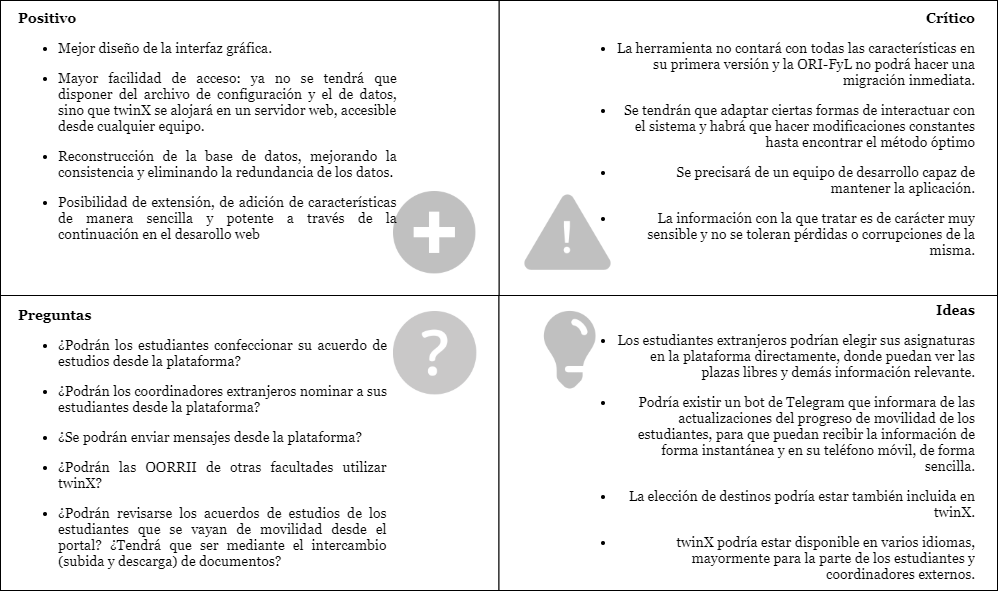
\includegraphics[width=\textwidth]{img/malla.png}
	\caption{Malla receptora de la información}
	\label{fig:malla}
\end{figure}


\section{Descripción de la propuesta}
Una vez hemos dado pinceladas de todo lo que tenemos, de qué podemos hacer, qué no y cómo llevarlo a cabo, vamos a establecer los claros objetivos de este proyecto y definir exactamente cuál será el producto tras su finalización, una vez conocemos todo el entorno que lo rodea. 

\subsection{Elección del tipo de metodología de desarrollo}
\label{elecciónMetodología}
Para desarrollar twinX primero se ha de elegir una metodología. Tradicionalmente, los proyectos de software se construían siguiendo lo que se conocen como «metodologías pesadas» o tradicionales \cite{waterfall1}, largos procesos de desarrollo en los que se definen unas fases secuenciales por donde el producto iba pasando hasta tener una versión final. La metodología más sonada es la de «cascada» o \textit{waterfall} en inglés \cite{waterfall2}. En ella, tenían lugar unas estrictas etapas enfocadas a un grupo de tareas en concreto, como son la etapa de definición, la de diseño, la de codificación, la de pruebas y la de mejora. Todo ello daba lugar a documentaciones muy completas aunque innecesariamente extensas en muchos casos, a través de la implicación de mucha gente experta en la materia, capacitada para hacer las tareas definidas muy concretamente. La flexibilidad apenas estaba contemplada, puesto que la planificación era muy estricta y hacía peligrar la buena continuidad del proyecto.

Hoy en día, apenas se utiliza este tipo de metodologías. En nuestro caso, queremos construir lo que sería tan sólo el comienzo del producto final. En otras palabras, nuestras condiciones no encajarían en una metodología en cascada, pues no tenemos unos requisitos estrictamente fijados, ya que vamos a crear una versión de TWINS no definitiva y la cual no se verá con todas las características implementadas. Además, es un cambio tan drástico el que se va a dar al transportar la aplicación a la web, que se precisa de la continua atención de una especie de «equipo supervisor», conformado por uno o varios usuarios finales del producto, que nos pueda proporcionar un \textit{feedback} sobre si nos estamos acercando o alejando de sus expectativas. Sobre esto último, diremos que no es que no se tuviera en cuenta en las metodologías tradicionales, pero no se primaba tanto como se debería, lo que hacía que el software perdiera calidad.

Por todo ello, podemos aventurarnos a decir que nuestro proyecto encaja más en una \textbf{metodología ágil}. Este tipo de metodologías se basan en la adaptación a medios con necesidades cambiantes, con un desarrollo muy de cerca con el cliente, quien está presente junto con el equipo de desarrollo en las numerosas reuniones que se hacen a lo largo de la vida del proyecto. Es más, en el \textit{14th Annual State of Agile Report} \cite{stateofagile} podemos encontrar unas estadísticas sobre los beneficios que ha traído el uso de metodologías ágiles en el último año, entre las que podemos destacar la capacidad de manejar los cambios de prioridades, la reducción de riesgos en el proyecto o el mantenimiento del software. En este caso, el equipo de desarrollo es ajustado, pero no por ello dejaremos de lado la necesaria intervención de dos personas fundamentales que hacen el papel de clientes y que son:

\begin{itemize}
	\item María Consuelo Pérez Ocaña (Coordinadora de Internacionalización en la la Facultad de Filosofía y Letras)
	\item Miguel Ángel Sanz Sáez (personal de secretaría y creador de TWINS)
\end{itemize}

\subsection{Propuesta de producto}
\label{propuesta}
En su primera versión, twinX incluirá la funcionalidad mínima de TWINS, de modo que de cara a las pruebas, la interacción con la nueva plataforma sea más bien realista, y aporte verosimilitud a la mejora, pudiendo así ser tomada como tal.

Más concretamente, contemplamos la implementación de:

\begin{itemize}
	\item El añadido, modificación y eliminación de información esencial (como son asignaturas, tipo de expediente --similar a \gls{ExpedienteTWINS}--, mensajes predefinidos, etc.)
	\item La visualización de la información relevante a estudiantes (sus datos personales, expedientes abiertos, fases de los mismos, etc.)
	\item La visualización de los \glspl{Convenio}, modificación de la información y el añadido de nuevos. Posibilidad de dos vistas: una de resumen y otra completa, tal y como se tiene en TWINS.
	\item Calendario con eventos, tareas, tal y como se disponía en TWINS
	\item El envío de mensajes, a modo de sustituir los avisos en TWINS, pero abriendo el abanico a tres tipos de mensaje: mensaje normal, recordatorio (mensaje de un usuario para sí mismo) y avisos (por proximidad a la fecha de un evento o al límite para realizar una determinada tarea).
	\item Una pantalla inicial de visualización de la información de mayor relevancia a modo de resumen. 
	\item Organización de todo el contenido en tres grandes secciones: «gestión», «calendario» y «panel de control», para simplificar y mejorar la interfaz de usuario, facilitando la interacción con la misma.
	\item Búsqueda en los distintos listados (convenios, estudiantes, expedientes...) con filtros para facilitar la recuperación de la información.
\end{itemize}

\section{Presupuesto}

\section{Planificación}
\subsection{La metodología Scrum}
En relación con la sección ~\ref{elecciónMetodología}, la metodología concreta a usar para el desarrollo de twinX será \textbf{Scrum}. Es ideal para incrementar la flexibilidad y producir un sistema que pueda responder ante tanto requisitos iniciales como los que se van añadiendo a lo largo del proceso de desarrollo que se puedan ir descubriendo.

En Scrum, se asume que el análisis, el diseño y los procesos de desarrollo son impredecibles, y por ello, tienen que ser iterativos; esto es, hay que estar constantemente comprobando el trabajo realizado, evaluando qué se ha hecho, para adaptarlo de la mejor manera posible a la situación del proyecto. Esta repetición recibe el nombre de \textbf{sprint}, y es una medida de esta metodología.

Los sprints son flexibles y no lineales. Se podrían tomar como una caja negra que precisa de controles externos. De este modo, en cada iteración se pueden tener en cuenta todos los factores que se crean necesarios, de forma que se evite convertir el proceso en algo caótico y que se aleje de los objetivos del proyecto y, al mismo tiempo, se pueda maximizar la flexibilidad. \cite{scrum}

Vamos a agrupar en tres bloques las fases de la metodología Scrum:
\begin{itemize}
	\item \textbf{Preparación.} Podemos diferenciar dos subfases:
	\begin{itemize}
		\item Planificación: donde se estiman el coste y el tiempo del proceso
		\item Arquitectura: para decidir cómo se van a implementar los elementos de la lista de trabajos pendientes o \textit{backlog}
	\end{itemize} 
	\item \textbf{Desarrollo:} donde se lleva a cabo la realización de los sprints acordados en la fase anterior. Se desarrollan nuevas funcionalidades, respetando las variables del tiempo, requisitos, calidad, coste y competición. El fin de esta fase está condicionado a cuán bien se interacciona con las variables mencionadas.
	\item \textbf{Finalización:} preparación para el lanzamiento del producto, donde se incluye la documentación final, y unas pruebas que se realizan con anterioridad a la versión final del software.
\end{itemize}

\subsection{Planificación en sprints}

A continuación, vamos a exponer la planificación que se ha pensado para llevar a cabo el desarrollo de este producto piloto para la plataforma twinX, de acuerdo con lo expuesto en la sección ~\ref{propuesta}:

\subsubsection*{\textbf{Sprint 0: puesta a punto}}

\begin{itemize}
	\item \textbf{Toma de decisiones acerca del renombramiento de algunas entidades existentes en TWINS:} existen una serie de nombres que pueden ser confusos para una persona que trate de comprender el funcionamiento de TWINS desde cero; si bien esto no ocurre con los usuarios habituales de la aplicación de Access\textregistered, con el desarrollo de twinX estamos, por lo general, facilitando a todo el entorno de la ORI-FyL, y por tanto, se renombrará alguna entidad como por ejemplo «evento». El motivo no es otro que la confusión entre un evento de calendario cotidiano y un \gls{EventoExpedienteTWINS}. Para ello, se tiene que hacer un segundo análisis de la base de datos ya creada y así poder mejorar la comprensión de nuevos usuarios en la plataforma.
	\item \textbf{Realización de un tutorial de \textit{Yii2 Framework}:} sobre los detalles de la tecnología a usar para el desarrollo de twinX hablaremos en la sección ~\ref{implementacion}. Sin embargo, antes de ponernos manos a la obra con la implementación del sistema web, habrá que adquirir los conocimientos necesarios para la toma de buenas decisiones y el respeto de las buenas prácticas del framework. %PENDIENTE
	\item \textbf{Modelado de la base de datos:} realizar el diseño lógico-conceptual de la base de datos es esencial a la hora del desarrollo. Una vez se tiene, podemos crear las tablas necesarias para hacer funcionar la aplicación. Es de suma importancia dedicar el tiempo suficiente a esta tarea, dado que los  errores en el modelo pueden dar lugar a imprevistos temporales en el futuro.
	\item \textbf{Creación de bocetos:} necesarios para confeccionar las interfaces de usuario sobre un esquema ya pensado, de modo que las decisiones de diseño de importancia tengan lugar en esta fase, y no sobre la marcha, ya que es más costoso en cuanto a tiempo y la consistencia de las vistas puede verse comprometida.	
\end{itemize}


\subsubsection*{\textbf{Sprint 1: comienzo del desarrollo}}

\begin{itemize}
	\item \textbf{Integrar el \gls{paneltwinX}:} desde donde se añadirán nuevos registros a la plataforma, del lado del \gls{superusuario}. Es la parte más importante si tenemos en cuenta que es la que nos posibilita hacer pruebas de la manera más sencilla, ya que no se espera que twinX tenga en su primera versión ninguna herramienta de migración masiva de datos. 
	%PARA LA SECCIÓN 4
%	\begin{itemize}
%		\item \textbf{Integrar la vista de usuarios}	
%		\item \textbf{Integrar la vista de fases de expediente}
%		\item \textbf{Integrar la vista de mensajes predefinidos}
%		\item \textbf{Integrar la vista de países}
%		\item \textbf{Integrar la vista de universidades}
%	\end{itemize}

	\item \textbf{Integrar el módulo de \gls{gestiontwinX}:} como parte fundamental de twinX, donde se tiene la mayor parte de la funcionalidad y las acciones que los \glspl{gestortwinX} llevarán a cabo durante su jornada laboral a diario, pues viene siendo el corazón del actual TWINS.
	%PARA LA SECCIÓN 4
%	\begin{itemize}
%		\item \textbf{Integrar la vista de convenios}	
%		\item \textbf{Integrar la vista de asignaturas}
%		\item \textbf{Integrar la vista de estudiantes}
%		\item \textbf{Integrar la vista de expedientes}
%		\item \textbf{Integrar la vista de tutores}
%	\end{itemize}
	
\end{itemize}

\subsubsection*{\textbf{Sprint 2: complementando twinX}}

\begin{itemize}
	\item \textbf{Integración del módulo de calendario:} el cual tendrá los mismos elementos que el calendario en TWINS, con eventos, tareas asociadas a los mismos, y avisos, en forma de mensaje, para las fechas límite de las tareas.
	\item \textbf{Integración del módulo de mensajería:} para el intercambio de mensajes o notas, en sustitución del confuso menú de la figura \ref{fig:avisos}
\end{itemize}

\subsubsection*{\textbf{Sprint 3: ensanchando horizontes}}

\begin{itemize}
	\item \textbf{Integrar el \textit{frontend} del estudiante:} con acciones básicas como el registro y la confección del acuerdo de estudios.
	\item \textbf{Integrar el \textit{frontend} del tutor:} para interaccionar con sus estudiantes y poder revisar sus acuerdos de estudios.
\end{itemize}

\subsubsection*{\textbf{Sprint 4: haciendo twinX aún más potente}}

\begin{itemize}
	\item \textbf{Integración del reconocimiento de créditos:} para los estudiantes salientes, trasladar sus puntuaciones obtenidas en su universidad de destino a calificaciones ponderables en su expediente en la UGR.
	\item \textbf{Integración de la alteración de matrícula:} proceso mediante el cual los estudiantes entrantes pueden tener asignadas sus asignaturas, confeccionados sus horarios dependiendo de factores como las plazas vacantes o el posible solapado de clases en un tramo horario.
	\item \textbf{Funcionalidad de migración de datos masiva:} desde la sede de la UGR, quien comunica a la ORI-FyL los listados de los estudiantes de movilidad entrantes y salientes.
\end{itemize}

Todas estas tareas pueden ser, acorde con la metodología Scrum, modificadas y trasladadas a otros sprints. Sobre las subtareas que conllevaría cada épica\footnote{Las épicas son tareas que almacenan dentro de ellos un gran número de subtareas.} (las expuestas anteriormente), hablaremos en la sección ~\ref{diseñoTécnico}. %PENDIENTE

Independientemente de la división del trabajo en todos estos sprints, no se contempla la realización de más de uno o dos de ellos, con la posibilidad de cambiar los contenidos de los mismos, pues también habría que incluir la realización de las pruebas y la redacción de esta memoria.

En adición a la planificación aquí expuesta, cabe señalar la utilización de un tablero \textbf{Kanban}, característico de las metodologías ágiles y de Scrum. En él, se disponen las tareas en varias columnas. A cada tarea se le puede asignar un color para distinguirlo, por ejemplo, en los distintos sprints. Para la construcción de twinX hemos usado la herramienta \textit{Trello} para la confección de un tablero interactivo (figura \ref{fig:kanban}). Las distintas etiquetas representan distintos sprints, y a cada tarea (consideradas en su mayoría como épicas), se les puede adjuntar una lista de tipo \textit{checkbox} para asegurarnos de que no queda tarea sin hacer dentro de cada épica.

\begin{figure}
	\centering
	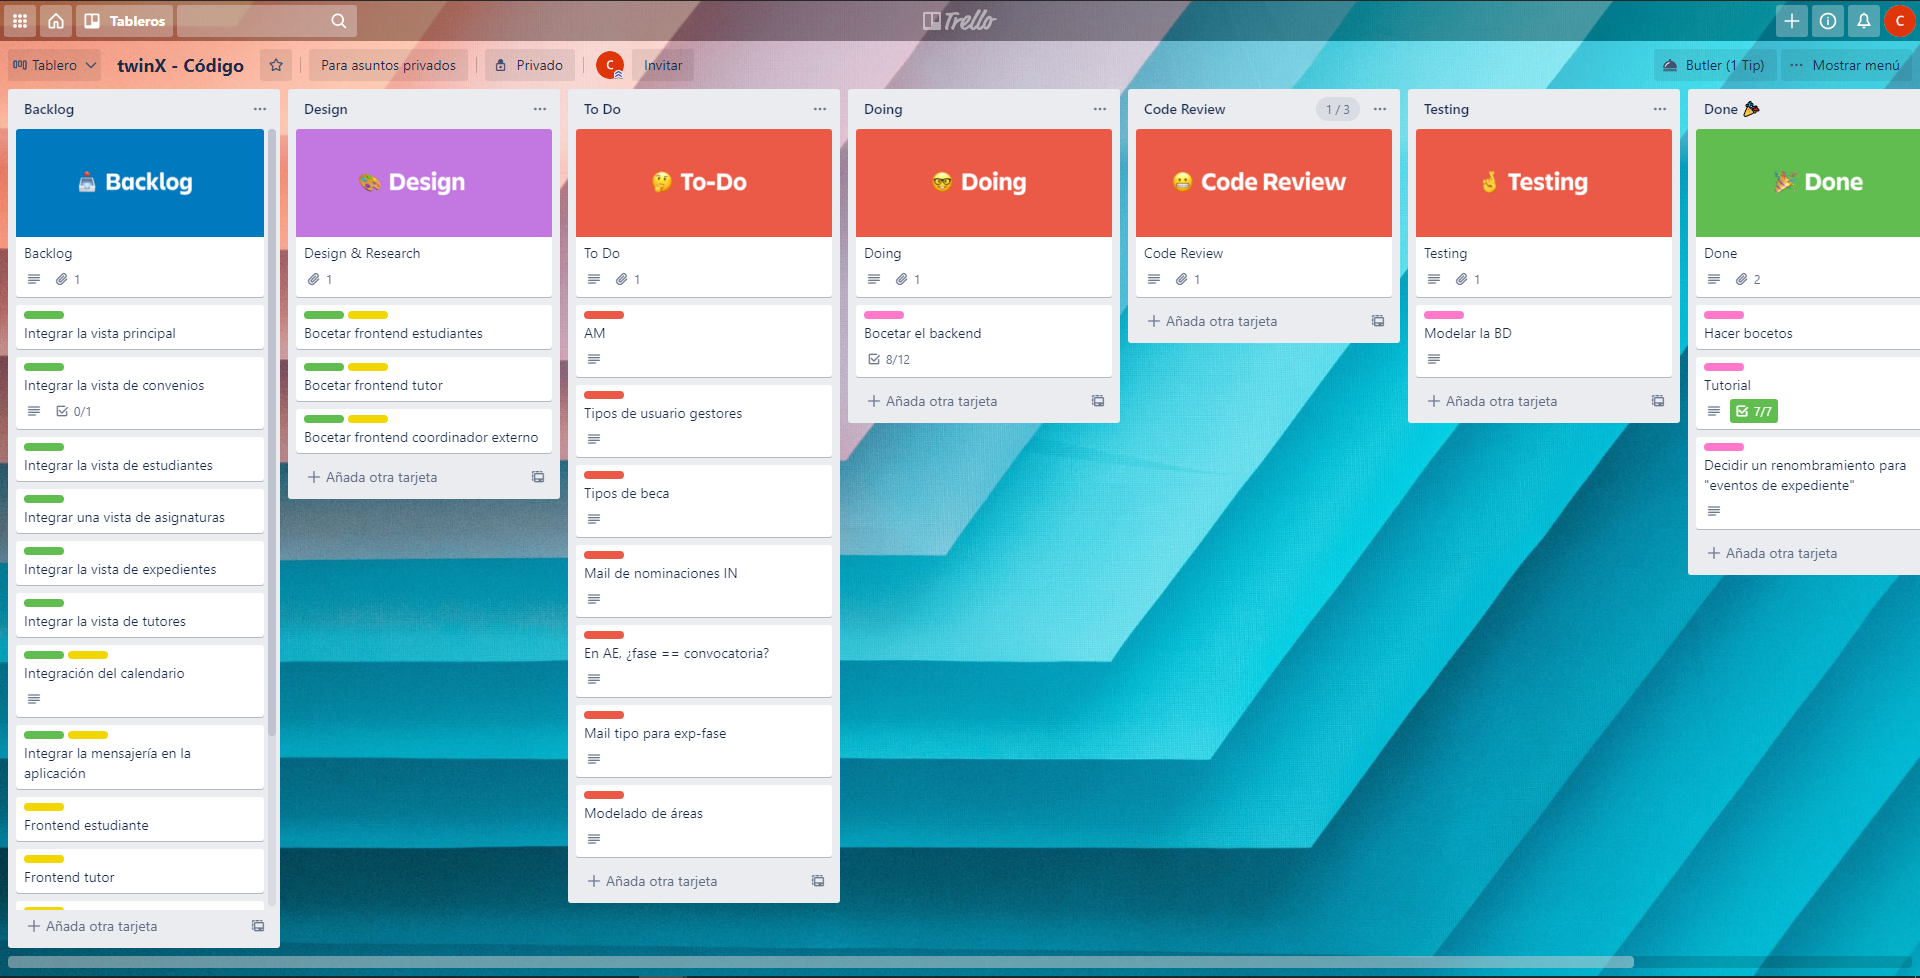
\includegraphics[width=\textwidth]{img/Capturas Kanban/kanban_codigo}
	\caption{Kanban al comienzo del desarrollo}
	\label{fig:kanban}
\end{figure}



% 4. Diseño de la interfaz de usuario

\chapter{Diseño de la interfaz de usuario}

Una vez hemos definido cuáles son nuestros objetivos, analizado el estado del arte y establecido unas pautas para el desarrollo, vamos a comenzar con el diseño de la parte visual. Esto es, a su vez, un proceso que requiere de distintas definiciones, de manera que al término de este capítulo, no sólo tengamos el diseño de las interfaces de usuario, sino que también comprendamos por qué se han diseñado así y la intención de cada elemento que disponemos en pantalla.

\section{Matriz de tareas de usuario}

Un buen comienzo sería el de definir los roles de usuario en nuestra nueva aplicación. Hemos hablado ya en el capítulo anterior sobre la figura del \gls{gestortwinX} y la del \gls{administradortwinX}. Incluyamos entonces también las de \gls{Tutor}, estudiante y, de forma excepcional, la de coordinador(a) externo/a. Sobre esta última, recordemos que no tenía ningún tipo de interacción en TWINS y que hasta entonces, los usuarios de la plataforma habían establecido intercambios de información por correo electrónico con los coordinadores de otras facultades, que es el método estándar de realizar las \glspl{Nominacion}. Sin embargo, aunque no para sus primeras versiones, se espera que twinX brinde la capacidad de hacer estas nominaciones a través de una interfaz gráfica, de una forma mucho más sencilla y segura que con el envío de un texto libre, donde puede haber errores y/o malas prácticas, dado el amplio uso que se puede hacer de la herramienta.

Es precisamente por la necesidad de dejar claras las acciones a llevar a cabo por cada usuario del sistema por la que elaborar una \textbf{matriz de tareas de usuario}. Esta herramienta nos permite establecer cuál es la frecuencia de uso de una característica de nuestra aplicación por un grupo de usuarios en concreto y cuál es la prioridad que debemos darle a la implementación de la misma. De esta forma, nos será más fácil diferenciar aquellas acciones que tan solo se lleven a cabo unas pocas veces al mes (o cada varios meses) y cuales, por el contrario, son ejecutadas casi a diario, de modo que se priorice su integración y su optimización. Sobre estas últimas, cabe decir que el potenciarlas no solo se procurará hacer en términos de procesamiento interno del código, sino también en cuanto a su facilidad de utilización por parte del usuario. Es decir, tendremos que crear más accesos directos o simplificar lo máximo posible el curso de tareas a llevar a cabo para realizar estas acciones y obtener los resultados deseados. En adición a todo esto, podremos observar cuáles son los usuarios que menos usarán la plataforma, de modo que se reste prioridad a la implementación de sus interacciones, en beneficio de las que llevan a cabo los usuarios que, por el contrario, monopolizan el uso de la aplicación. \cite{matrizTareas}

Para simplificar la matriz (tabla \ref{tab:matrizTareas}) y hacerla visualmente más sencilla de entender, vamos a asignar una serie de letras que correspondan a un nivel de utilización en concreto. Elegiremos la «A» para una frecuencia de uso alta, «M» para un uso medio y «B» para una baja frecuencia. A estas indicaciones añadiremos unas puntuaciones que nos permitirán determinar con mayor facilidad cuáles son las tareas de mayor importancia y cuáles son menos urgentes de implementar, al igual que los usuarios que desempeñarán un papel más o menos crítico en la aplicación. Respectivamente serán 3, 2 y 1 punto, de modo que las prioridades más altas recibirán una mayor puntuación y viceversa.

\begin{table}[h]
	\begin{center}
		\begin{adjustbox}{width=1\textwidth}
		\begin{tabular}{ | >{\centering\arraybackslash}p{0.375\linewidth} | c | c | c | c | c | c | } 
			\hline
			\textbf{Usuarios / Tareas} & \textbf{Administrador} & \textbf{Gestor} & \textbf{Tutor} & \textbf{Estudiante} & \textbf{Coordinador externo} & \textbf{Puntuación} \\
			\hline
			Acceder a twinX & M & A & B & B & B & \cellcolor{red!25}8 \\
			\hline
			Ver expedientes de un usuario & A & A & & & & \cellcolor{red!25}6 \\
			\hline
			Cambiar de fase un expediente & A & A & & & & \cellcolor{red!25}6 \\ 
			\hline
			Consultar la información de un convenio & A & A & & & & \cellcolor{red!25}6 \\ 
			\hline
			Modificar los datos de un estudiante & M & M & & B & & \cellcolor{red!25}5 \\
			\hline
			Introducir un nuevo convenio & B & M & & & & 3 \\
			\hline
			Realizar el acuerdo de estudios & & & & B & & 1 \\
			\hline
			Revisar propuesta de acuerdo de estudios & & B & M & & & 3 \\
			\hline
			Consultar los expediente pendientes de procesamiento & M & A & & & & 5 \\
			
			\hline
			Expresar consentimiento de cesión de datos & & & & B & & 1 \\
			\hline
			Añadir un nuevo tipo de expediente y/o fase de expediente & B & & &  & & 1 \\
			\hline
			Marcar un expediente como favorito & B & M & & & & 3 \\
			\hline	
			\textbf{Puntuación del grupo de usuarios} & \cellcolor{red!25}18 & \cellcolor{red!25}22 & 3 & 4 & 1 &  \\
			\hline
	\end{tabular}

	\end{adjustbox}
		\caption{Matriz de tareas de usuario}
		\label{tab:matrizTareas}
	\end{center}
\end{table}

Tras la atenta observación de la matriz, podemos afirmar que las acciones que mayor uso van a tener por los usuarios de twinX serían las ya existentes en TWINS, como es lógico, y que por supuesto, los grupos de usuarios con mayor necesidad de uso de la aplicación son los gestores y administradores. Sobre éstos últimos, cabe señalar que son una especie de gestores con más permisos de lo normal, de modo que pueden modificar la información que clasifica la situación de los estudiantes como son, por ejemplo, las fases de los expedientes. Solo los administradores podrían hacerlo, ya que los gestores no tienen por qué tener acceso a dichas modificaciones; simplemente necesitan trabajar con las ya registradas y, en caso de necesitar más entradas o la modificación de otras existentes, tendrían que solicitarlo a los administradores.

Con esta matriz, además, justificamos que el contenido de la primera versión de twinX (descrito en la sección ~\ref{propuesta}), es suficiente para cubrir la mayoría de las necesidades esenciales del trabajo de un secretario de la ORI-FyL, lo que es uno de los objetivos principales de este proyecto, aunque sea tan solo un comienzo a lo que finalmente llegaría a ser twinX.

\section{Sitemap}
\section{Labelling (iconografía)}
\section{Bocetos wireframe}

\subsection{Wireframes del módulo de gestión}

\begin{figure}
	\centering
	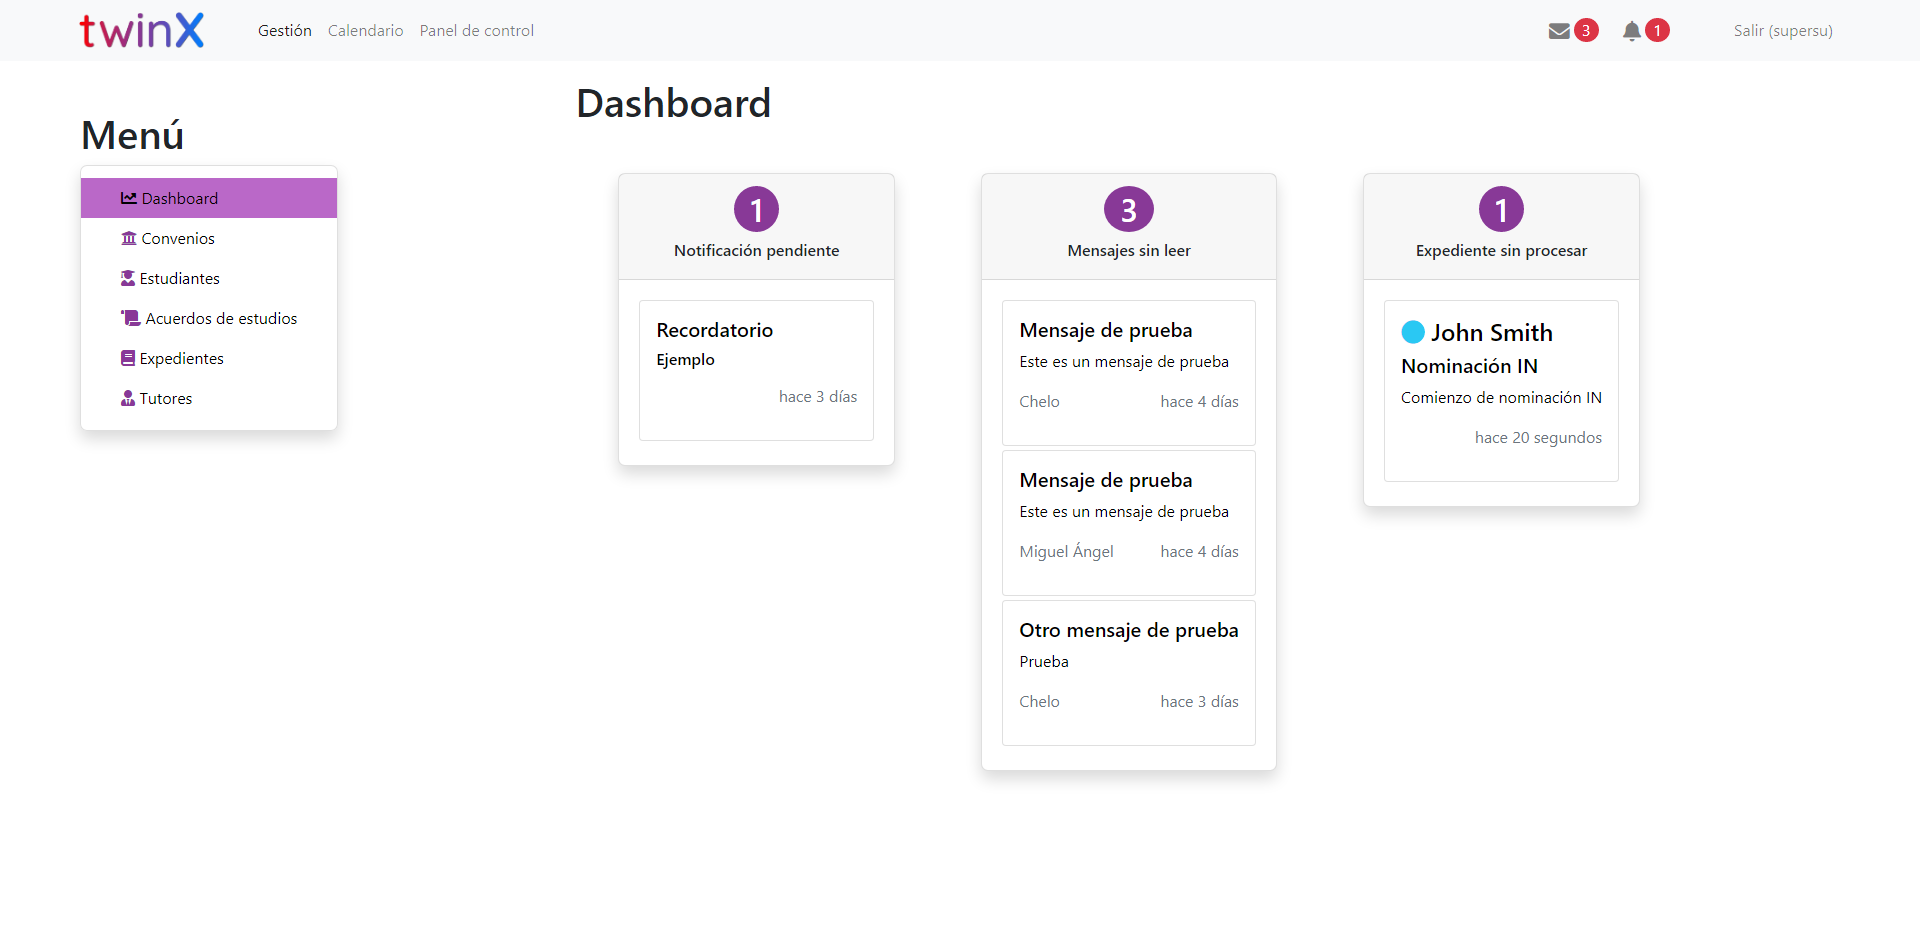
\includegraphics[width=\textwidth]{img/Wireframes/Gestión/dashboard.png}
	\caption[Wireframe de \textit{Dashboard}]{Wireframe del \textit{Dashboard} donde el usuario verá de un vistazo toda la información de mayor importancia al iniciar la aplicación}
	\label{fig:dashboardWF}
\end{figure}

\begin{figure}
	\centering
	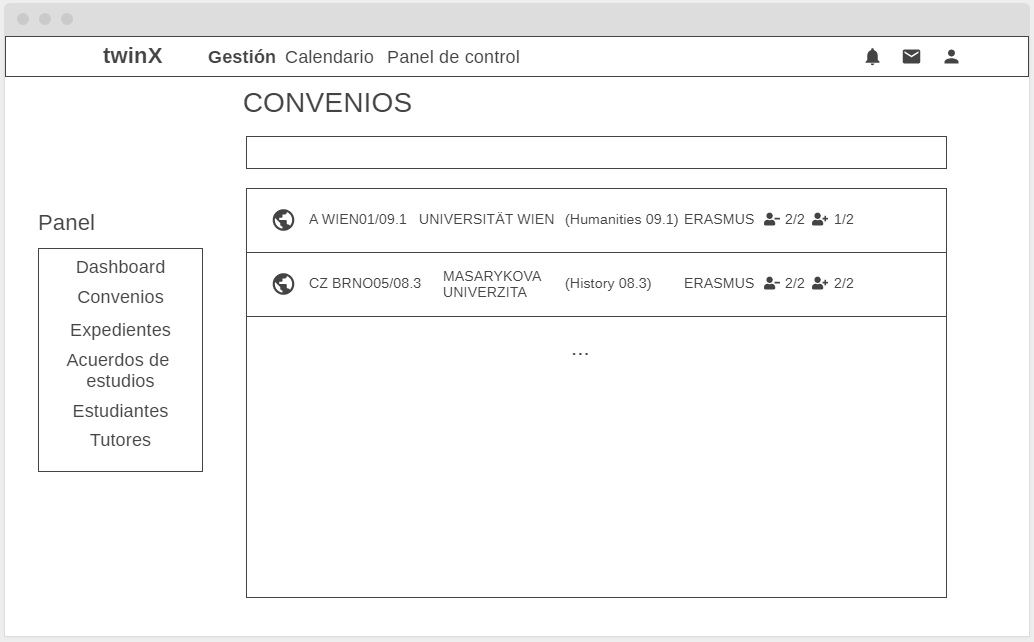
\includegraphics[width=\textwidth]{img/Wireframes/Gestión/convenios_lista.png}
	\caption{Wireframe de lista de convenios}
	\label{fig:convenios_listaWF}
\end{figure}

\begin{figure}
\centering
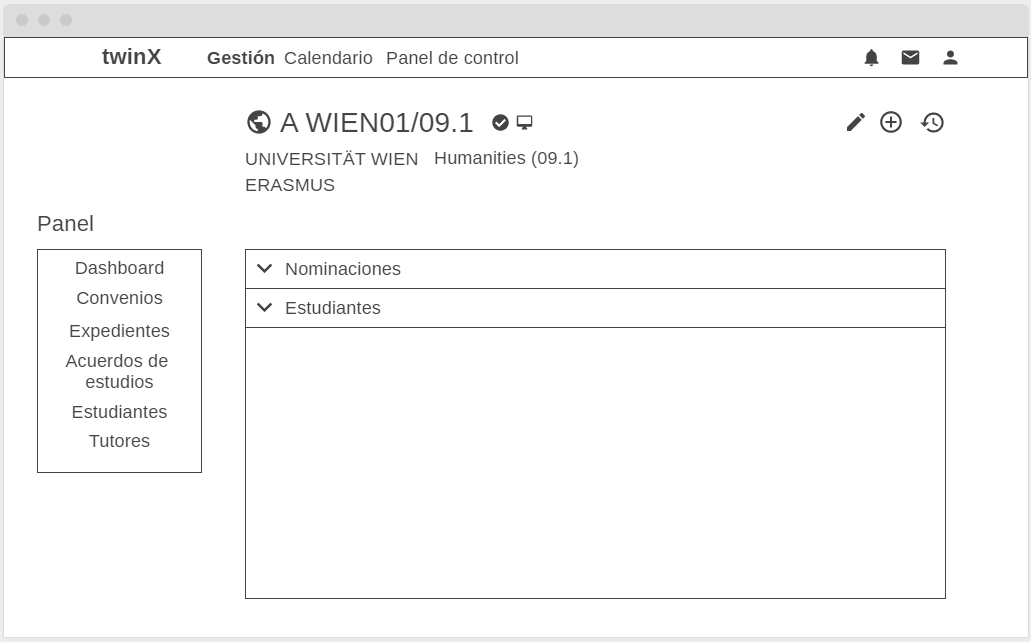
\includegraphics[width=\textwidth]{img/Wireframes/Gestión/vista_convenio_básica_contraída.png}
\caption[Wireframe de vista de convenio básica]{Wireframe de vista de convenio básica. Secciones contraídas.}
\label{fig:vista_conv_básica_contWF}
\end{figure}

\begin{figure}
	\centering
	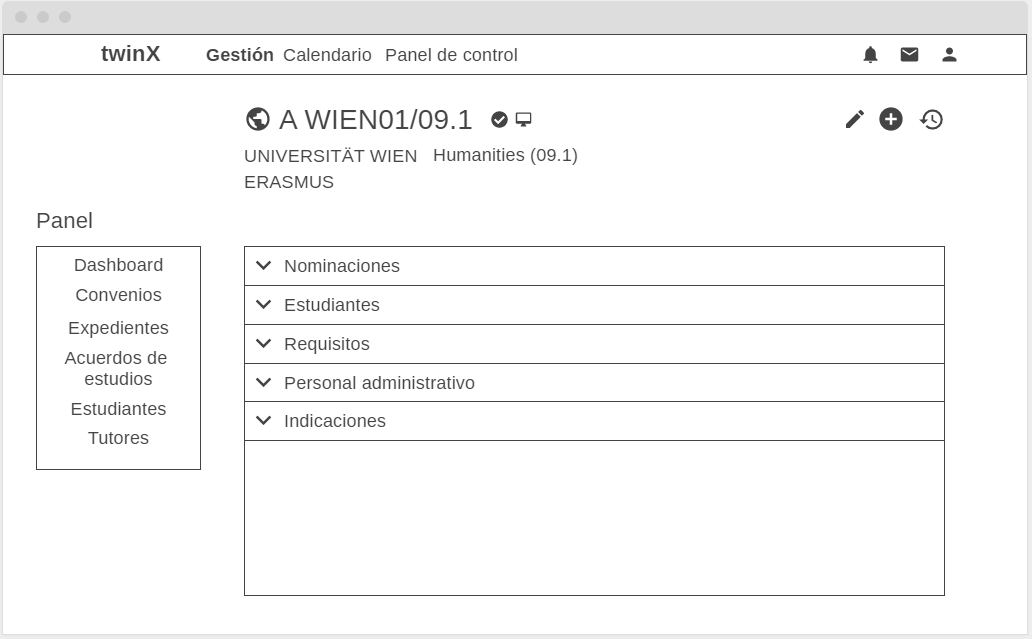
\includegraphics[width=\textwidth]{img/Wireframes/Gestión/vista_convenio_avanzada_contraída.png}
	\caption[Wireframe de vista de convenio avanzada]{Wireframe de vista de convenio avanzada. Secciones contraídas. Acceso desde el botón «+» de la botonera en la esquina superior derecha del contenido principal.}
	\label{fig:vista_conv_avanzada_contWF}
\end{figure}

\begin{figure}
	\centering
	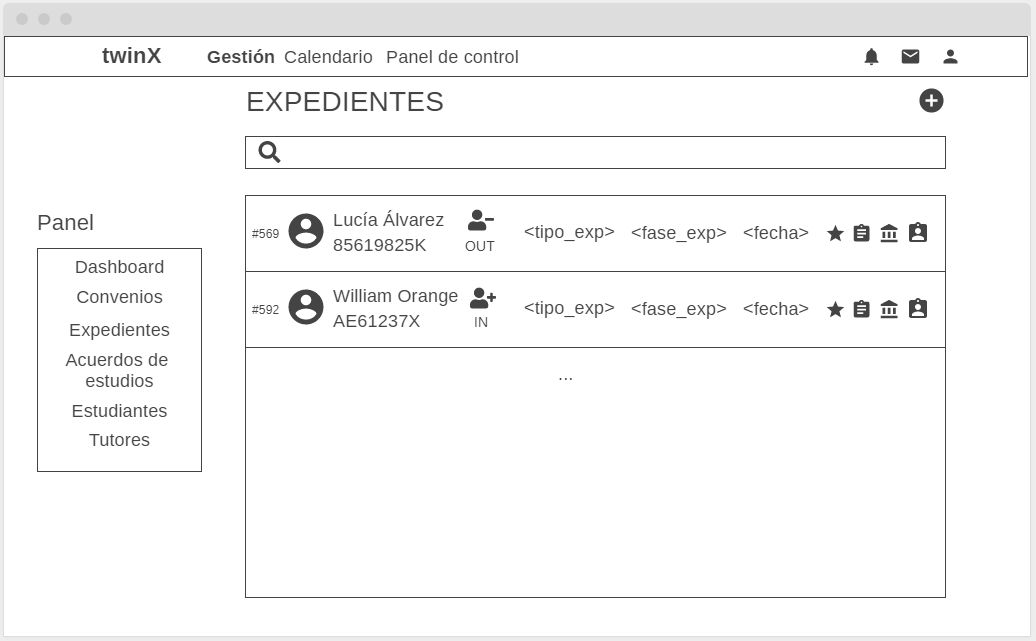
\includegraphics[width=\textwidth]{img/Wireframes/Gestión/expedientes_lista.png}
	\caption{Wireframe de lista de expedientes}
	\label{fig:expedientes_listaWF}
\end{figure}

\begin{figure}
	\centering
	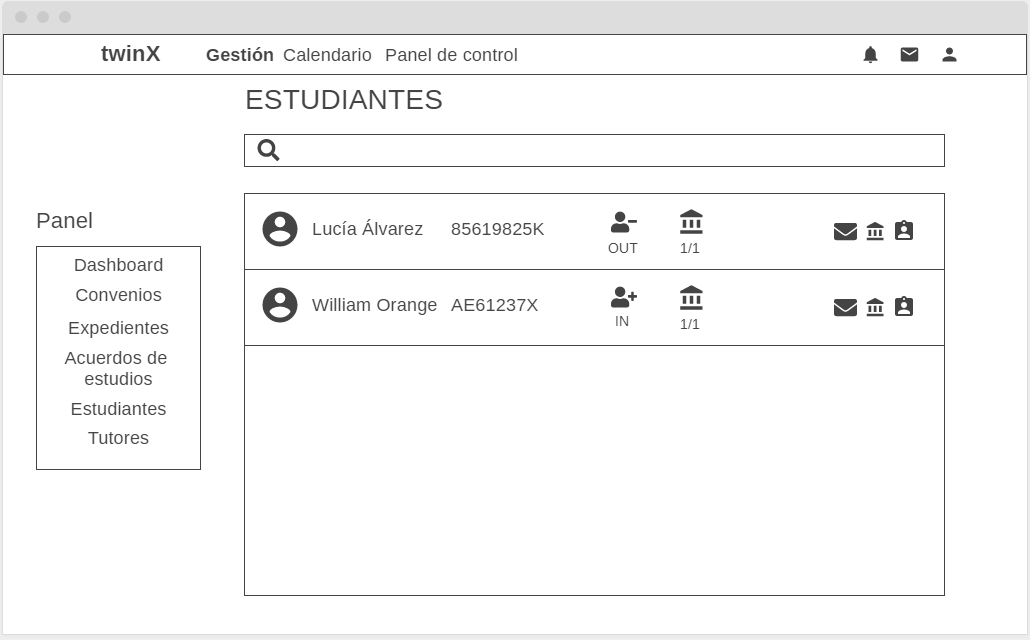
\includegraphics[width=\textwidth]{img/Wireframes/Gestión/estudiantes_lista.png}
	\caption{Wireframe de lista de estudiantes}
	\label{fig:estudiantes_listaWF}
\end{figure}

\begin{figure}
	\centering
	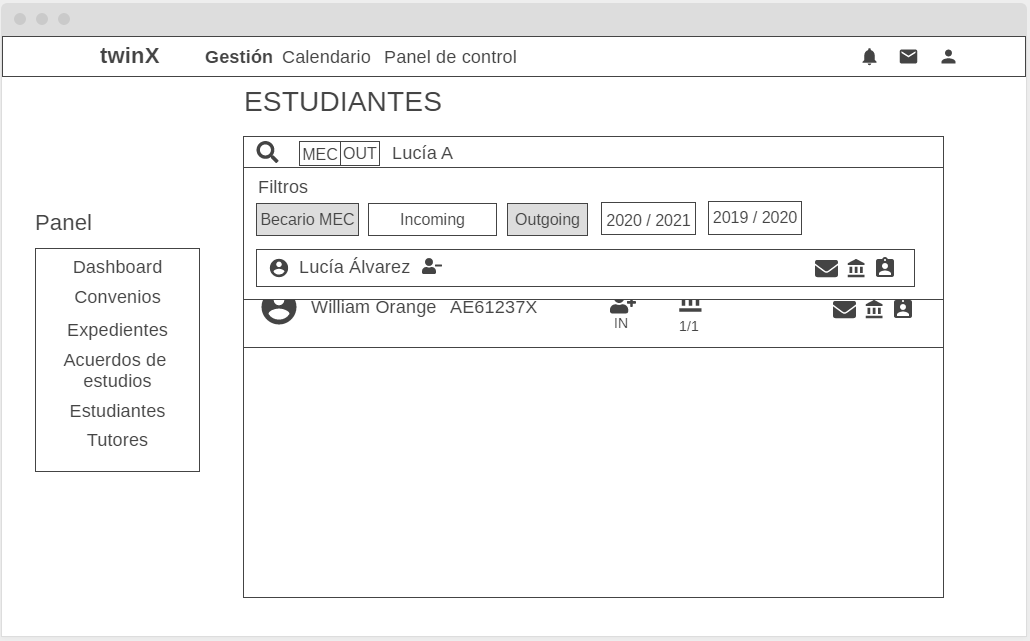
\includegraphics[width=\textwidth]{img/Wireframes/Gestión/búsqueda.png}
	\caption[Wireframe de búsqueda]{Wireframe de búsqueda. Diálogo modal, desplegable desde la barra. Capacidad de filtrado}
	\label{fig:búsquedaWF}
\end{figure}

\begin{figure}
	\centering
	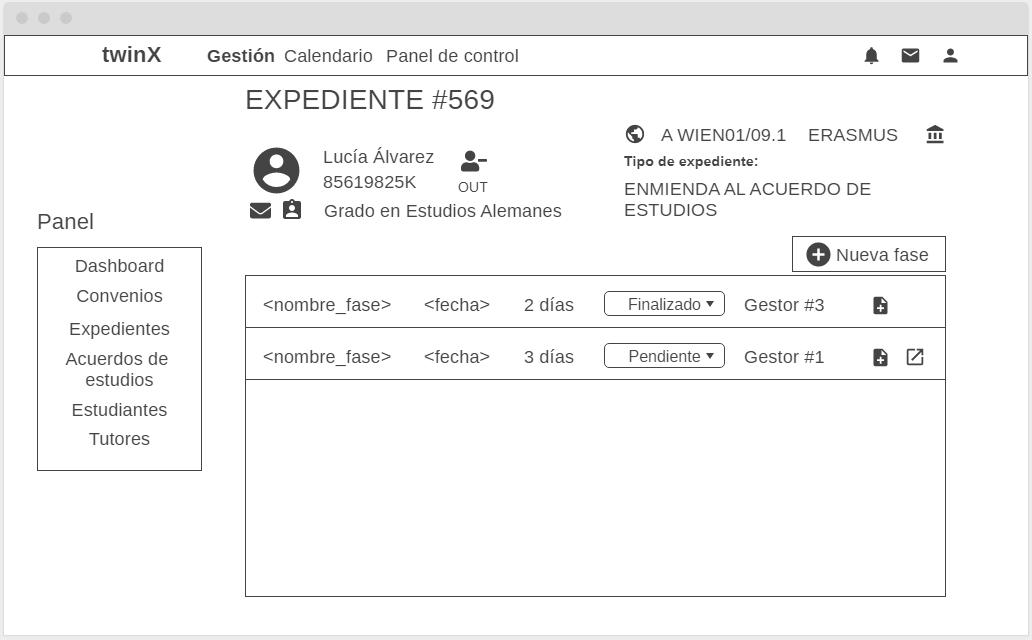
\includegraphics[width=\textwidth]{img/Wireframes/Gestión/expediente_detalle.png}
	\caption{Wireframe de detalle de expediente}
	\label{fig:expediente_detalleWF}
\end{figure}

\begin{figure}
	\centering
	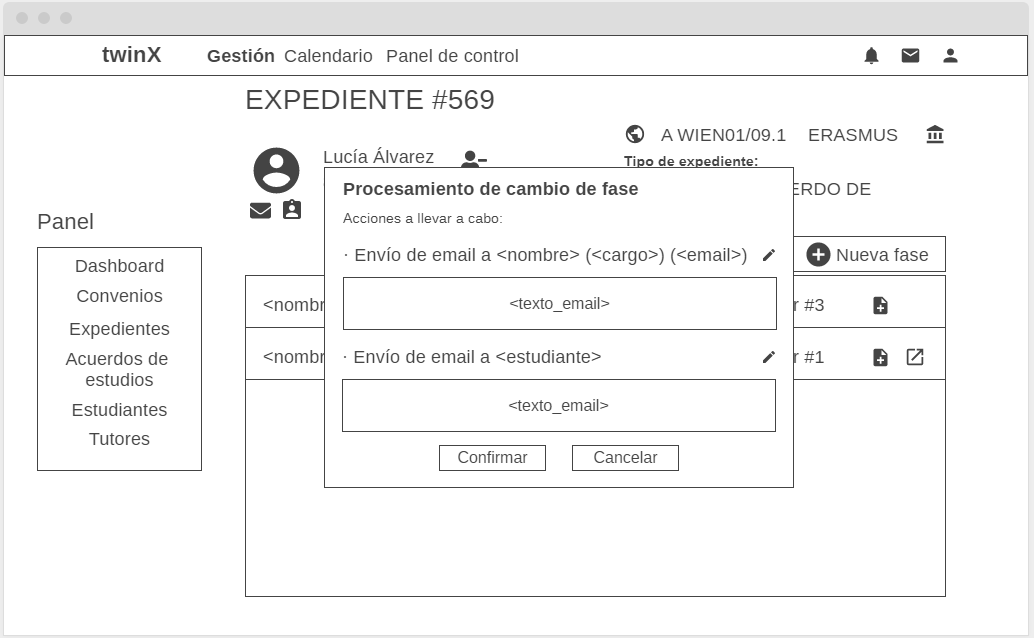
\includegraphics[width=\textwidth]{img/Wireframes/Gestión/cambio_fase.png}
	\caption[Wireframe del modal de cambio de fase]{Wireframe del modal de cambio de fase. Advierte sobre las acciones a llevar a cabo tras la tramitación del cambio de fase en un expediente concreto.}
	\label{fig:cambio_faseWF}
\end{figure}

\begin{figure}
	\centering
	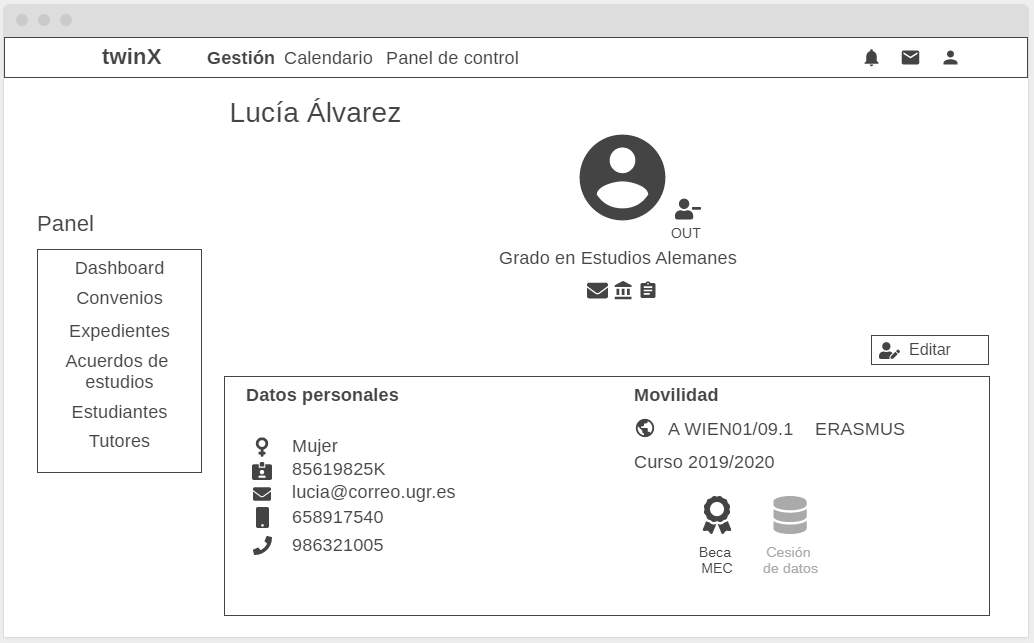
\includegraphics[width=\textwidth]{img/Wireframes/Gestión/estudiante_detalle.png}
	\caption{Wireframe de la vista de detalle de un estudiante}
	\label{fig:estudiante_detalleWF}
\end{figure}

%%PROVISIONAL PARA SEPARAR AMBOS CONJUNTOS DE WIREFRAMES
\newpage

\subsection{Wireframes del módulo de calendario}

\begin{figure}
	\centering
	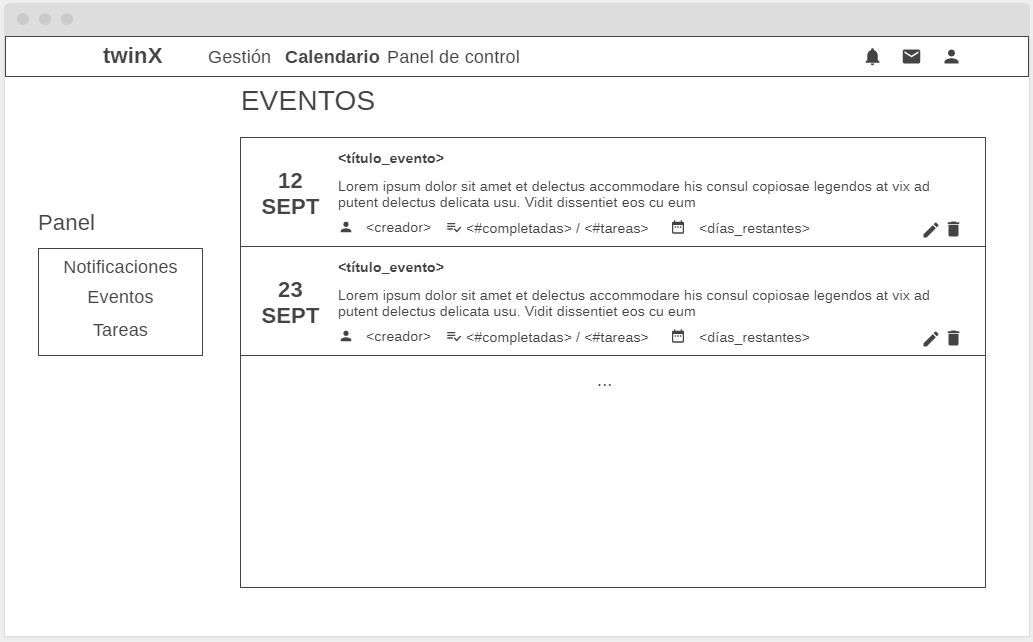
\includegraphics[width=\textwidth]{img/Wireframes/Calendario/eventos_lista.png}
	\caption{Wireframe de lista de eventos}
	\label{fig:eventos_listaWF}
\end{figure}

\begin{figure}
	\centering
	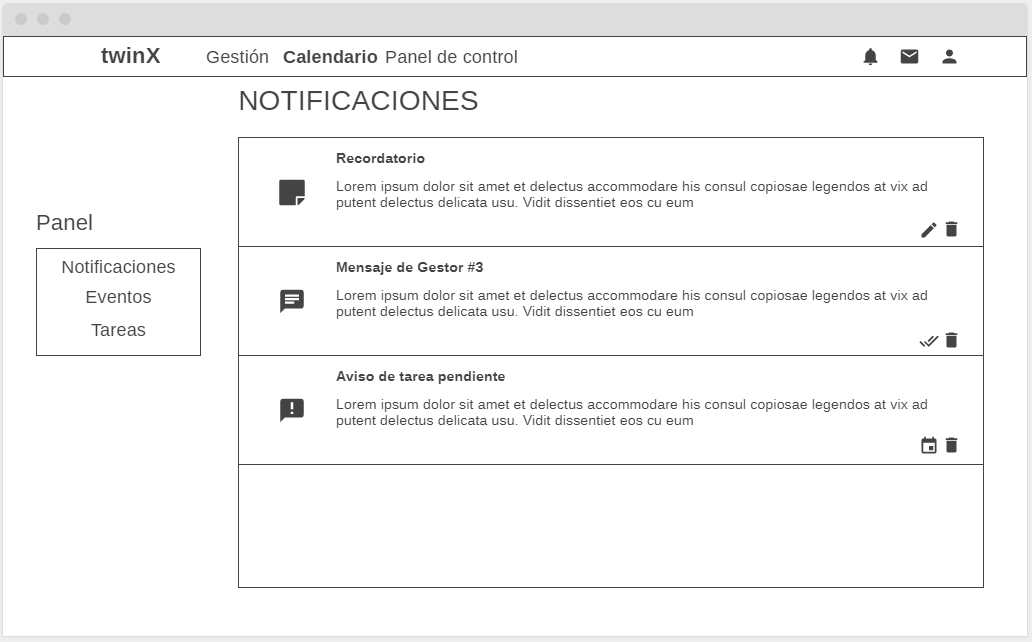
\includegraphics[width=\textwidth]{img/Wireframes/Calendario/notificaciones_lista.png}
	\caption[Wireframe de lista de notificaciones]{Wireframe de lista de notificaciones. Pueden aparecer tres tipos de notificaciones, dependiendo del tipo de mensaje recibido o generado por la propia plataforma (a través de avisos y/o recordatorios)}
	\label{fig:notificaciones_listaWF}
\end{figure}

\begin{figure}
	\centering
	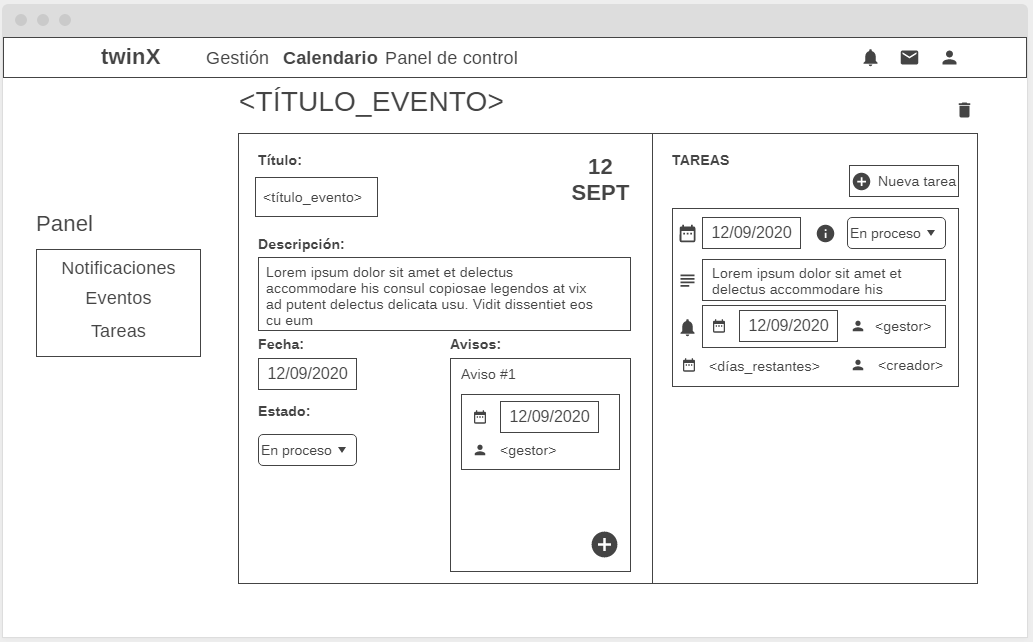
\includegraphics[width=\textwidth]{img/Wireframes/Calendario/nuevo_evento.png}
	\caption[Wireframe de creación de un evento]{Wireframe de creación de un evento. Se distinguen dos vistas: la información del evento en general (izquierda) y la de sus subtareas (derecha)}
	\label{fig:nuevo_eventoWF}
\end{figure}





% 5. Diseño técnico

\chapter{Diseño técnico}

Hemos definido hasta ahora gran parte de los ingredientes que llevará twinX: quiénes lo van a usar, qué es capaz de hacer, cuánto vamos a tardar en hacerlo y por qué hace falta algo como twinX.

Es hora de ponernos manos a la obra. Pero antes de ello, es necesario aún definir muchas más cosas, todo ello en relación con lo anterior pero a más bajo nivel: cuáles van a ser exactamente nuestras tareas, qué subtareas asociadas tendremos que desarrollar y cómo va a ser la base de datos. Será vez puestos todos los ingredientes a nuestra disposición para cocinarlos cuando podamos comenzar a utilizar nuestras herramientas para conseguir nuestro objetivo.

\section{Listado inicial del producto (product backlog)}

Es cierto que ya sabemos lo que va a ser capaz de hacer twinX en su primera versión, pero no tenemos claros los pequeños pasos a dar para poder completar las grandes tareas que ya conocemos. Por ello, vamos a elaborar un listado de todo lo que tenemos que hacer en orden de preferencia, paso a paso, para poder conseguir nuestros objetivos de manera organizada.

La priorización de la lista de tareas suele estar hecha por el llamado \textit{product owner}; esto es, el propietario del producto final (en este caso, las dos personas mencionadas en la sección ~\ref{eleccionMetodologia}). Sin embargo, en este caso, vamos a obviar la labor de los propietarios, dado que no se está construyendo un producto desde cero, sino que se parte de lo que ya se construyó en TWINS y porque además, la intención de este proyecto no es obtener un producto inmediatamente utilizable, sino como propuesta de donde partir.

Más técnicamente, cada uno de los componentes de esta lista son acciones que el usuario podrá desarrollar. Esto es algo característico de Scrum y su constante enfoque en el usuario, todo ello en relación con su activa participación con el equipo de desarrollo durante todo el proceso. Pues bien, estas capacitaciones que el usuario final tendrá reciben el nombre de \textbf{historias de usuario}, y es la forma que se tiene en esta metodología ágil de nombrar a los clásicos requisitos. Suponen una reducción en la documentación, ya que no se necesitan especificar demasiados elementos a priori. No obstante y como ya comentamos en secciones pasadas, el número de tareas y, por tanto, de historias de usuario, puede variar, pues al comienzo de cada sprint se realiza una reunión para evaluar los trabajos del equipo de desarrollo y se vuelve a revisar la priorización que se ha hecho de las tareas en el \textit{product backlog}.

En referencia a esas «grandes tareas» que hemos mencionado anteriormente y que ya tenemos definidas, podríamos decir que dentro de ellas se esconden otras pequeñas tareas que nos son más sencillas de seguir a la hora del desarrollo. Es decir, son historias de usuario encerradas en otra más grande que alberga a todas ellas. Esto se conoce en el argot de Scrum como \textbf{épicas}. Así, «hacer uso del panel de control» sería una épica, pues dentro de ella irían historias de usuario como «ver un listado con todos los tipos de expedientes».

En la tabla \ref{tab:listadoHU} encontramos el backlog genérico del desarrollo, como producto de la síntesis que se puede hacer de las secciones~\ref{subsec:propuesta} y~\ref{subsec:sprints}, donde hemos incluido las historias de usuario a desarrollar para la primera versión de twinX, en sus épicas correspondientes. Entendemos que todas las historias numeradas como «x.1», «x.2», ..., «x.n» pertenecen todas a la épica (historia de usuario) «x». Recordemos también que el significado de «historia de usuario» no es otro que una acción a desarrollar por el usuario final del sistema, por lo que siempre tienen que estar descritas desde su punto de vista. Es asunto del desarrollador el cuestionarse las tareas (de código en su mayoría) que implica realizar cada una de ellas, por lo que para la elaboración del backlog no nos centraremos en esas tareas a llevar a cabo en cuanto a implementación, sino a satisfacción de las necesidades del usuario.

\begin{table}[h]
	\begin{center}
		\begin{adjustbox}{width=1\textwidth}
			\begin{tabular}{ | c | >{\centering\arraybackslash}p{0.75\linewidth} | c | } 
				\hline
				\textbf{Identificador} & \textbf{Descripción} & \textbf{Sprint} \\
				\hline
				HU.1 \label{HU1} &  Acceso al panel de control & 1 \\
				\hline
				HU.1.1 \label{HU1.1} & Listado de usuarios en todo el sistema: consulta, búsqueda, edición y eliminación de registros. & 1 \\
				\hline
				HU.1.2 \label{HU1.2} & Listado de tipos de expedientes almacenados: consulta, búsqueda, edición y eliminación de registros. & 1 \\
				\hline
				HU.1.3 \label{HU1.3} & Listado de fases de expedientes almacenadas: consulta, búsqueda, edición y eliminación de registros. & 1 \\
				\hline
				HU.1.4 \label{HU1.4} & Listado de mails predefinidos almacenados: consulta, búsqueda, edición y eliminación de registros. & 1 \\
				\hline
				HU.1.5 \label{HU1.5} & Listado de universidades almacenadas: consulta, búsqueda, edición y eliminación de registros. & 1 \\
				\hline
				HU.1.6 \label{HU1.6} & Listado de países almacenados: consulta, búsqueda, edición y eliminación de registros. & 1 \\
				\hline
				HU.2.1 \label{HU2.1} & Ver la información más importante y de atención prioritaria de un vistazo & 1 \\
				\hline
				HU.2.2 \label{HU2.2} & Gestionar los estudiantes: listado y vistas independientes con posibilidad de edición de sus datos & 1 \\
				\hline
				HU.2.3 \label{HU2.3} & Gestionar los convenios: listado y vistas independientes con posibilidad de edición de los distintos campos & 1 \\
				\hline
				HU.2.4 \label{HU2.4} & Gestionar los expedientes de los estudiantes: listado y vistas independientes con posibilidad de modificar sus fases & 1 \\
				\hline
				HU.2.5 \label{HU2.5} & Gestionar los acuerdos de estudios: listado y vistas independientes con posibilidad de consultar los estudiantes relacionados y sus datos & 1 \\
				\hline
				HU.2.6 \label{HU2.6} & Ver todos los tutores del sistema y consultar los acuerdos de estudios asociados a los mismos & 1 \\
				\hline
				HU.3 \label{HU.3} & Planificación de eventos y tareas & 2 \\
				\hline
				HU.3.1 \label{HU.3.1} & Crear nuevos eventos con tareas asociadas a los mismos & 2 \\
				\hline
				HU.3.2 \label{HU.3.2} & Configurar avisos de los eventos y tareas que se creen & 2 \\
				\hline
				HU.3.3. \label{HU.3.3} & Configurar recordatorios personales & 2 \\
				\hline
				HU.4 \label{HU.4} & Hacer uso de una mensajería entre los usuarios & 2 \\
				\hline
				HU.4.1 \label{HU.4.1} & Consultar y borrar los mensajes recibidos y poder escribir nuevos & 2 \\
				\hline			
			\end{tabular}	
		\end{adjustbox}
		\caption{Listado de historias de usuario}
		\label{tab:listadoHU}
	\end{center}
\end{table}

\begin{table}[h]
	\begin{center}
		\begin{tabular}{ | c | c | c | } 
			\hline
			
			\hline			
		\end{tabular}	
		\caption{HU1}
		\label{tab:HU1}
	\end{center}
\end{table}





% 6. Implementación

\chapter{Implementación}
\label{implementacion}

Hasta ahora, con todas las piezas de información que hemos generado acerca del desarrollo, hemos podido, en efecto, discernir entre tres grandes grupos de tareas: la gestión, el calendario y el panel de control. Así pues, estableceremos la separación del desarrollo en estos tres grandes bloques de trabajo, con la previa especificación de las herramientas a utilizar y del trabajo anterior al comienzo del proceso de programación, propiamente dicho, que implican la puesta a punto de la base de datos y del servidor para probar y desarrollar nuestra aplicación.

\section{Herramientas para el desarrollo de twinX}

Para llevar a cabo la programación de este sitio web, aunque utilicemos herramientas más sofisticadas, éstas están basadas en los clásicos lenguajes web: \textbf{HTML} (\textit{HyperText Markup Language}) \cite{html} para la estructuración de la web y la identificación de los distintos elementos, \textbf{CSS} \cite{css} (\textit{Cascading Style Sheets}) para aplicar estilo a la vista (posicionamiento, colores, visibilidad, etc.) y JavaScript \cite{javascript}, para implementar funciones más complejas a cada componente de la web. Para el manejo de estos dos últimos, contaremos con la ayuda de dos librerías con un gran potencial. Para el estilo, usaremos \textbf{Bootstrap} \cite{bootstrap} en su cuarta versión y para JavaScript utilizaremos \textbf{jQuery} \cite{jquery}. Nos permitirán ahorrar mucho tiempo, ya que en ambos casos podemos hacer uso de funciones o palabras clave que evitarán el tener que escribir numerosas líneas de código en cada uno de los lenguajes a los que complementan.

Como ya hemos mencionado en varias ocasiones, el desarrollo va a ser llevado a cabo con la ayuda de \textbf{Yii2 Framework}\footnote{Sus siglas significan \textit{Yes, it is!}}. En su segunda versión, este framework hace uso del lenguaje de programación PHP para orquestar múltiples tareas que resultan engorrosas de llevar a cabo sin su ayuda y que pueden extenderse demasiado, como son, por ejemplo, las operaciones con la base de datos o la generación de código del que partir para dar forma a la vista, modelo o controlador de alguna de las secciones de twinX \cite{yii}. Hoy en día, en proyectos de desarrollo, sería muy complicado prescindir de una herramienta como esta, ya que las alternativas son numerosas y completas.

Entre sus características, destacamos el generador de código \textbf{Gii} (figura \ref{fig:gii}), que puede automatizar la creación, por ejemplo, de la clase de un modelo, o incluso de una tabla CRUD al completo (esto es, su vista y su controlador). Tan solo tenemos que indicar cuál es la tabla de la base de datos sobre la que queremos generar los fragmentos de código, y atendiendo a las restricciones creadas en la misma, se puede obtener fácilmente una clase instanciable para recuperar o guardar información en su tabla. Del mismo modo, al crear una tabla CRUD, tendríamos directamente en nuestro sitio web una interfaz donde pueden verse los registros almacenados en la base de datos, con la posibilidad de crear nuevos, eliminarlos o incluso filtrarlos y editarlos. No cabe duda del potencial de esta característica, la cual nos permitirá ahorrar mucho tiempo y seguridad a la hora de desarrollar y de depositar la confianza en código automáticamente generado y sin errores.

\begin{figure}
	\centering
	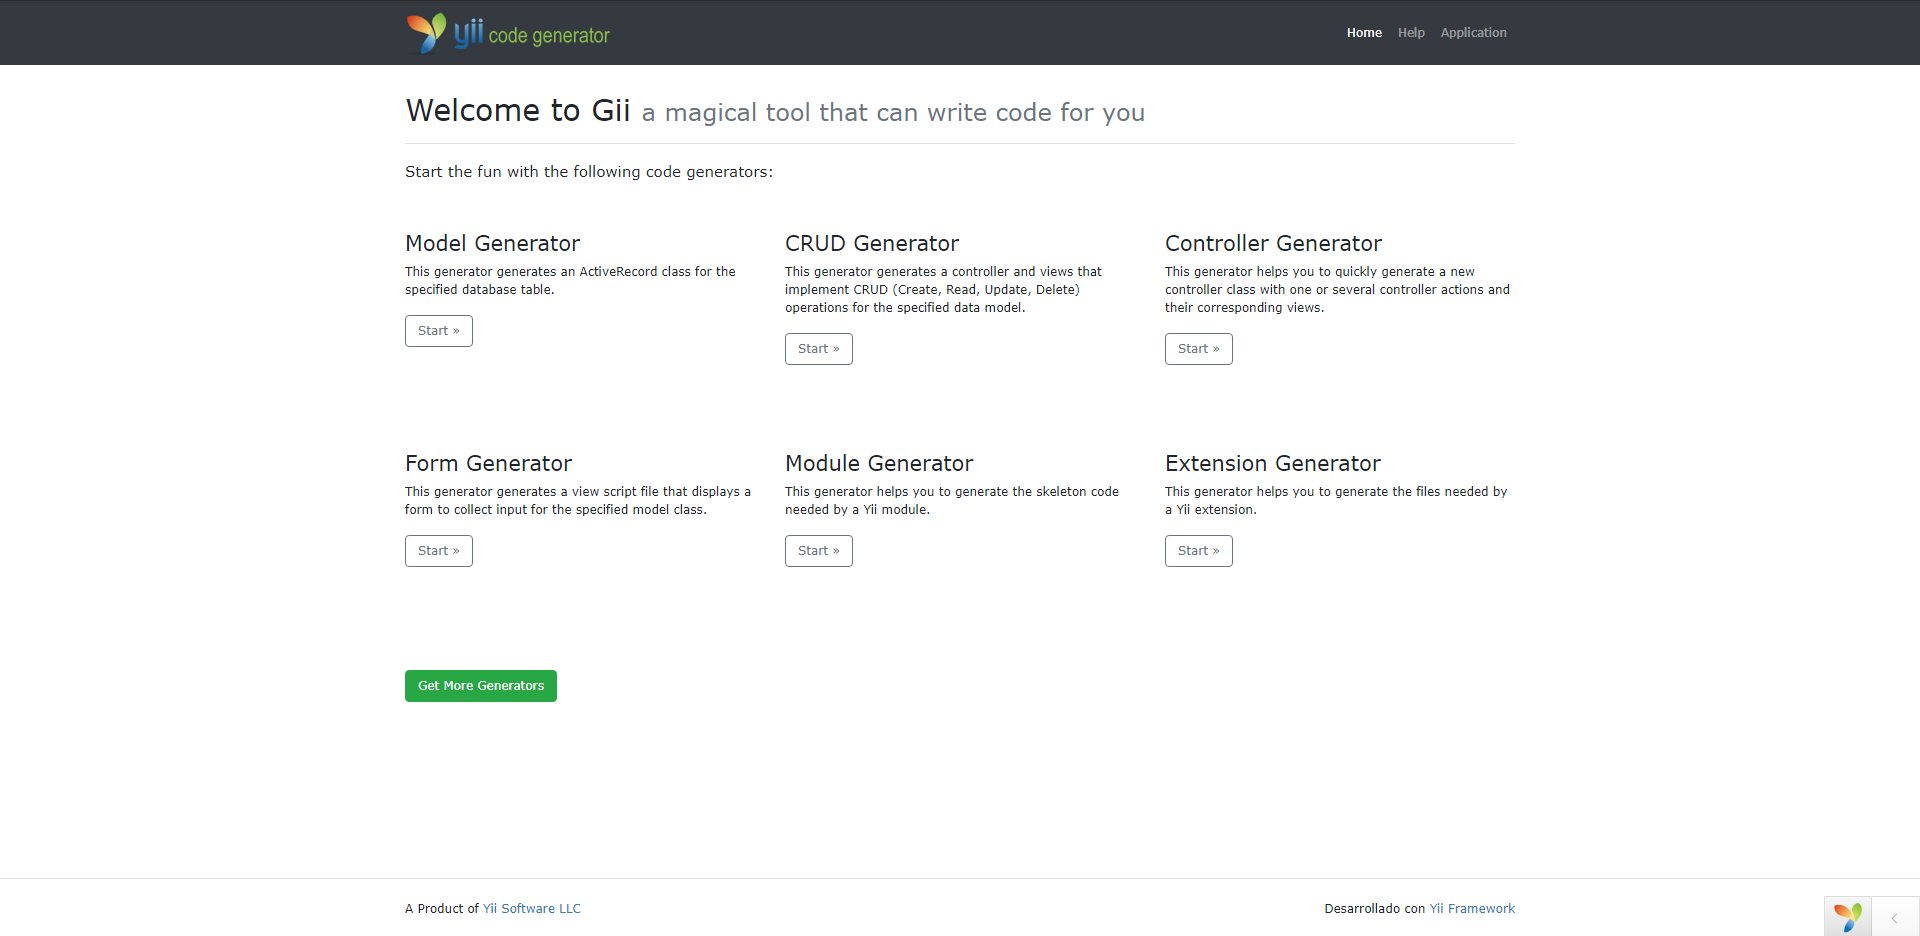
\includegraphics[width=\textwidth]{gii}
	\caption[Portal de Gii]{Portal de Gii desde donde podemos seleccionar un tipo de elemento a crear para que genere su código fuente}
	\label{fig:gii}
\end{figure}


Para comenzar a usar Yii, lo primero que tenemos que hacer es hacernos con el gestor de dependencias de PHP \textbf{Composer} \cite{composer} y descargarnos el esqueleto de un proyecto en Yii2 avanzado \cite{yii2advanced}. Para ello, basta con escribir:

\par\noindent\rule{\textwidth}{0.4pt}\linebreak
\\
\texttt{composer create-project --prefer-dist yiisoft/yii2-app-advanced twinX}
\par\noindent\rule{\textwidth}{0.4pt}

Y con ello ya tendríamos la carpeta con nuestro proyecto. Concretamente este directorio es el que tenemos que servir y al que nos conectaremos para visualizar nuestra web. También tenemos que seguir los pasos en el repositorio de GitHub de yiisoft para aplicar los ajustes necesarios derivados del renombramiento y redireccionamiento de URLs en el servidor. Además, tendremos que instalar algunas dependencias haciendo uso de la orden \texttt{composer install} y de iniciar el entorno de desarrollo con el archivo \texttt{ini} de PHP que incluye el repositorio que hemos clonado.

A continuación, procederemos con la instalación de la pila software \textbf{XAMPP} (Apache, MariaDB, PHP y Perl). En Windows, es una instalación sencilla a través de una interfaz de usuario, por lo que no requiere un gran tiempo. Es importante que, una vez instalado, situemos la carpeta del proyecto dentro del directorio \texttt{htdocs}, en la raíz de la carpeta de instalación de xampp. Se recomienda instalar en el directorio C:\ en Windows. En nuestro caso, hemos hecho los ajustes necesarios para poder situar esta carpeta en otro directorio desde donde se trabaja con el repositorio GitHub del proyecto, para que de forma más cómoda podamos salvaguardar el progreso del desarrollo de forma periódica sin tener que copiar archivos de un directorio que esté fuera del repositorio.

Esta pila contiene la aplicación \textbf{phpMyAdmin}, que ha sido también una gran ayuda para poder visualizar las tablas en base de datos, acceder a registros concretos o ejecutar código MySQL desde una interfaz gráfica. Frente a una terminal desde donde manejar la base de datos, presenta una menor tasa de errores al introducir órdenes, pues la información puede verse a golpe de click y con una presentación más vistosa.

Sobre GitHub, el repositorio se creó  al comienzo de la redacción de esta memoria \cite{repogit}, donde mediante la creación de ramas hemos ido guardando en distintos \textit{commits} las progresivas versiones del proyecto. Una vez creada una pieza de valor, se hacía una mezcla (\textit{merge}) a la rama \texttt{master}, de modo que cada rama se creaba con un fin, para añadir una nueva funcionalidad, sin depender del funcionamiento de las demás y que poco a poco se puedan ir integrando todas las características en su totalidad.

Finalmente, otro de los protagonistas del desarollo es el IDE\footnote{\textit{Integrated Development Environment}} con que se ha programado twinX. En este caso, haciendo uso de su licencia educativa, se ha usado \textbf{PhpStorm} \cite{phpstorm}. Ha sido esencial, pues hemos descartado otras herramientas como Visual Studio Code ya que no tienen tan buen integración con PHP y Yii en sí como tiene este IDE. Destacan también características como su guardado automático inteligente, su potente búsqueda de archivos y sus cómodos atajos de teclado. Todo ello han hecho el proceso de desarrollo muy cómodo y liviano.


\section{Creación de la base de datos}

Tal y como hemos indicado en la sección \ref{sec:modelobd}, para crear el esquema del modelo de la base de datos, hemos usado la herramienta \textbf{dbdiagram.io} \cite{dbdiagram}. Ésta tiene mucho potencial, pues no es un simple creador de diagramas. Su principal característica es la confección de la parte gráfica mediante una especie de lenguaje creado por los mismos creadores, \textbf{DBML} \cite{dbml}. Con él, se pueden especificar tablas, atributos, estructuras de enumeración y características de los atributos, como claves externas, primarias, cardinalidades y nulidad. Gracias a ello, se ha podido mejorar progresivamente el modelo de la base de datos, pues un cambio en el código implica una variación en la visualización de las tablas, bien sea con algún atributo de más o alguna nueva relación entre tablas.

No solo es posible ver con mayor claridad las características del modelo en el código en DBML, sino que también tiene la gran posibilidad de exportarlo a otro lenguaje como es MySQL. De este modo, con tan solo unos clicks, se obtienen las órdenes que posteriormente nuestra base de datos entenderá y podrá crear todas las tablas por nosotros, con todas las restricciones establecidas y ahorrando, así, mucho tiempo.

En la práctica, el código que tenemos en DBML para generar el modelo de la figura \ref{fig:modeloBD} es:

\lstset{breaklines=true}
\begin{lstlisting}
	// ENTIDADES BASICAS
	
	Table centro as CEN {
		id int [pk, increment]
		nombre varchar [not null, unique]
	}
	
	Table curso as CURSO {
		id int [pk, increment]
		curso varchar(4) [not null]
	}
	
	Table mail_predef as MAIL {
		id int [pk, increment]
		titulo varchar [not null, unique]
		asunto varchar [not null]
		cuerpo text [not null]
	}
	
	Table titulacion as TIT {
		id int [pk]
		nombre varchar [not null, unique]
		id_centro int [not null]
	}
	
	Ref: TIT.id_centro > CEN.id
	
	Table asignatura as ASIG {
		id int [pk]
		id_tit int [not null]
		nombre varchar [not null]
		ects int [not null]
		cuatrimestre cuatrimestre [not null]
		tipo tipo_asignatura [not null]
	}
	
	Ref: ASIG.id_tit > TIT.id
	
	Table asignatura_ext as EXT_ASIG {
		id int [pk]
		id_conv int [not null] 
		nombre varchar [not null]
		ects int [not null]
		id_curso int [ref: > CURSO.id, not null] 
		cuatrimestre cuatrimestre [not null]
	}
	
	Ref: EXT_ASIG.id_conv > CON.id
	
	Table pais as P {
		iso varchar [pk]
		nombre varchar [not null]
	}
	
	Table universidad as UNI {
		cod_uni varchar [not null]
		cod_pais varchar [not null]
		nombre varchar [not null]
		direccion varchar 
		web varchar
		email varchar
		
		Indexes {
			(cod_pais, cod_uni) [pk]
		}
	}
	
	Ref: UNI.cod_pais > P.iso
	
	Table area as AR {
		cod_isced varchar [pk]
		nombre_isced varchar [not null]
		nombre_area varchar 
		
	}
	
	// USUARIOS Y TIPOS
	
	Table user as U {
		id int [pk, increment]
		username varchar
		nombre varchar
		tipo tipo_usuario
		password varchar
		email varchar
		telefono varchar
		genero genero
	}
	
	Table estudiante as EST{
		id_usuario int [not null]
		dni varchar [not null, unique] // PUEDE SER NIE
		id_convenio int [not null]
		id_titulacion int [not null]
		telefono2 int 
		email_go_ugr varchar 
		f_nacimiento datetime [not null]
		tipo_estudiante tipo_estudiante [not null]
		cesion_datos boolean 
		nota_expediente double 
		beca_mec boolean
	}
	
	Ref: EST.id_titulacion > TIT.id
	Ref: U.id - EST.id_usuario
	Ref: EST.id_convenio > CON.id
	
	
	// CONVENIOS Y ACUERDOS
	
	Table competencia_ling as CL {
		id int [pk, increment]
		lengua varchar [not null]
		nivel nivel_idioma [not null]
	}
	
	Table rel_cl_est {
		id int [pk, increment]
		id_cl int [ref: > CL.id, not null]
		id_est int [ref: > EST.id_usuario, not null]
	}
	
	Table req_ling_conv {
		id int [pk, increment]
		id_comp int [ref: > CL.id, not null]
		id_conv int [ref: > CON.id, not null]
	}
	
	Table convenio as CON {
		id int [pk, increment]
		cod_area varchar [not null]
		cod_uni varchar [not null]
		cod_pais varchar [not null]
		id_admon_out int
		
		id_curso_creacion int [ref: > CURSO.id, not null]
		creado_por int [not null]
		
		num_becas_in int [not null]
		num_becas_out int [not null]
		
		meses_in int [not null]
		meses_out int [not null]
		
		anno_inicio int [not null]
		anno_fin int [not null]
		
		req_titulacion varchar
		req_curso varchar
		
		nominacion_online boolean 
		link_nom_online varchar 
		info_nom_online text
		
		link_documentacion varchar
		
		movilidad_pdi boolean 
		movilidad_pas boolean 
		
		tipo_movilidad tipo_movilidad [not null]
		
		user_online varchar
		password_online varchar
		fecha_online datetime
		
		info_tor text 
		
		observ_discapacidad text
		observ_req_ling text 
		
		begin_nom_1s datetime
		end_nom_1s datetime
		begin_nom_2s datetime
		end_nom_2s datetime
		begin_app_1s datetime
		end_app_1s datetime
		begin_app_2s datetime
		end_app_2s datetime
		begin_mov_1s datetime
		end_mov_1s datetime
		begin_mov_2s datetime
		end_mov_2s datetime
		
		memo_grading text
		memo_visado text
		memo_seguro text
		memo_alojamiento text
		
		nombre_coord varchar
		cargo_coord varchar
		email_coord varchar
		tlf_coord varchar
		address_coord varchar [note:"Por defecto igual que la de la universidad"]
		web_inf_acad varchar
		
		nombre_admon_in varchar
		cargo_admon_in varchar
		mail_admon_in varchar
		nombre_resp_acad_in varchar
		cargo_resp_acad_in varchar
		
		nombre_admon_out varchar
		cargo_admon_out varchar
		mail_admon_out varchar
		nombre_resp_acad_out varchar
		cargo_resp_acad_out varchar
		mail_resp_acad_out varchar
		
	}
	
	Ref: P.iso < CON.cod_pais
	Ref: CON.creado_por > U.id
	Ref: CON.cod_area > AR.cod_isced
	Ref: CON.(cod_pais, cod_uni) > UNI.(cod_pais, cod_uni)
	
	
	Table acuerdo_estudios as AE {
		id int [pk, increment]
		id_estudiante int [not null]
		id_tutor int [not null]
		
		timestamp_creacion datetime [not null]
		periodo cuatrimestre [not null]
		fase int [not null]
		id_curso int [ref: > CURSO.id, not null]
		necesidades text
		begin_movilidad date // comienzo individual del estudiante
		end_movilidad date // fin individual del estudiante
		timestamp_nominacion datetime 
		timestamp_registro datetime [not null]
		link_documentacion varchar
		n_solicitud_RRII int
		convocatoria convocatoria [not null]
	}
	
	Ref: AE.id_estudiante > EST.id_usuario
	Ref: AE.id_tutor > U.id
	
	Table ae_asigloc_asigext {
		id_ae int
		asig_loc int [ref: > ASIG.id]
		asig_ext int [ref: > EXT_ASIG.id]
		
		Indexes {
			(id_ae, asig_loc, asig_ext) [pk]
		}
	}
	
	Table renuncia as REN{
		id int [pk, increment]
		id_ae int  [not null, ref: - AE.id]
		descripcion text [not null]
		timestamp datetime [not null]
	}
	
	// EXPEDIENTES, TIPOS DE EXPDIENTE Y FASES
	
	Table expediente as EXP{
		id int [pk, increment]
		id_ae int [not null]
		id_tipo_exp int [not null]
	}
	
	Ref: EXP.id_ae > AE.id
	Ref: EXP.id_tipo_exp > TIPO_EXP.id
	
	Table tipo_expediente as TIPO_EXP {
		id int [pk, increment]
		descripcion varchar [not null]
		tipo_estudiante tipo_estudiante [not null]
	}
	
	Table fase_expediente as FAS_EXP {
		id int [pk, increment]
		id_tipo_exp int [not null]
		descripcion varchar [not null]
		fase_final boolean [default: 0]
	}
	
	Ref: FAS_EXP.id_tipo_exp > TIPO_EXP.id
	
	Table envio_mail_fase {
		id int [pk, increment]
		id_mail int [ref: > MAIL.id, not null]
		id_fase int [ref: > FAS_EXP.id, not null]
		cargo cargo [not null]
	}
	
	Table hist_envio_mail_fase {
		id int [pk, increment]
		id_mail int [ref: > MAIL.id, not null]
		id_fase int [ref: > FAS_EXP.id, not null]
		id_exp int [ref: > EXP.id, not null]
		email varchar [not null]
	}
	
	Table hist_envio_mail_fase_mod { // Mail modificado
		id int [pk, increment]
		asunto varchar
		cuerpo text [not null]
		id_fase int [ref: > FAS_EXP.id, not null]
		id_exp int [ref: > EXP.id, not null]
		email varchar [not null]
	}
	
	Table rel_exp_fase as REL_EF {
		id int [pk]
		id_exp int [not null]
		id_fase int [not null]
		id_gestor int [not null]
		procesado boolean 
		timestamp datetime [not null]
		info varchar
	}
	
	Ref: REL_EF.id_exp - EXP.id
	Ref: REL_EF.id_fase - FAS_EXP.id
	Ref: REL_EF.id_gestor - U.id
	
	Table rel_exp_fav_gestor { 
		id int [pk, increment]
		id_exp int [ref: > EXP.id]
		id_gestor int [ref: > U.id]
		//tipo_usuario == GESTOR
	}
	
	// CALENDARIO
	
	Table evento as EV {
		id int [pk, increment]
		id_creador int [not null]
		titulo varchar [not null]
		descripcion text
		estado estado_evento_tarea [not null]
		prioridad prioridad [not null, default: 'MEDIA']
	}
	
	Ref: EV.id_creador - U.id //tipo == GESTOR
	
	Table tarea as TASK {
		id int [pk, increment]
		descripcion text [not null]
		estado estado_evento_tarea [not null, default: 'PENDIENTE']
	}
	
	Table deadline_aviso as DLA { 
		id int [pk, increment]
		fecha datetime [not null]
		id_responsable int [not null]
		id_evento int  [not null]
		id_tarea int [not null]
	}
	
	Ref: DLA.id_responsable > U.id // tipo == GESTOR
	Ref: DLA.id_evento > EV.id
	Ref: DLA.id_tarea > TASK.id
	
	Table recordatorio {
		id int [pk, increment]
		timestamp datetime [not null]
		id_usuario int [ref: > U.id, not null]
		deadline datetime [not null]
		titulo varchar [not null]
		descripcion text
		completado boolean
	}
	
	
	// MENSAJES	
	Table mensaje as MSG{
		id int [pk, increment]
		timestamp datetime [not null]
		id_emisor int [not null]
		id_receptor int [not null]
		leido boolean
		etiqueta etiqueta_msg [not null]
		asunto varchar 
		cuerpo text [not null]
		
	}
	
	Ref: MSG.id_emisor > U.id
	Ref: MSG.id_receptor > U.id
	
	Enum tipo_asignatura {
		TRONCAL
		OBLIGATORIA
		OPTATIVA
	}
	
	Enum cargo {
		COORDINADOR
		ADMON_IN
		ADMON_OUT
		RESP_ADMON_OUT
	}
	
	Enum nivel_idioma {
		B1
		B2
		C1
		C2
	}
	
	
	Enum etiqueta_msg {
		IMPORTANTE
		ELIMINADO
	}
	
	Enum estado_evento_tarea {
		PENDIENTE
		EN_PROCESO
		TERMINADO
	}
	
	Enum prioridad {
		ALTA
		MEDIA
		BAJA
	}
	
	Enum estado_ae {
		REVISION
		DENEGADO
		ACEPTADO
		VIGENTE
	}
	
	Enum convocatoria {
		PRIMERA
		SEGUNDA
		EXTRAORDINARIA
	}
	
	Enum tipo_movilidad {
		ERASMUS
		ARQUS
		ERASMUS_DI
		ERASMUS_PARTNER
		INTERCAMBIO
		LIBRE_MOVILIDAD
	}
	
	Enum tipo_usuario {
		SUPERUSUARIO
		GESTOR
		ESTUDIANTE
		TUTOR
	}
	
	Enum genero {
		F
		M
		O
	}
	
	Enum tipo_estudiante {
		INCOMING
		OUTGOING
	}
	
	Enum cuatrimestre {
		PRIMERO
		SEGUNDO
		C_COMPLETO
	}
	
\end{lstlisting}

Y como resultado, podemos traducir todo ello a código MySQL, quedando de la siguiente manera:

\begin{minted}[frame=lines, breaklines]{mysql}
	
	CREATE TABLE `centro` (
	`id` int PRIMARY KEY AUTO_INCREMENT,
	`nombre` varchar(255) UNIQUE NOT NULL
	);
	
	CREATE TABLE `curso` (
	`id` int PRIMARY KEY AUTO_INCREMENT,
	`curso` varchar(4) NOT NULL
	);
	
	CREATE TABLE `mail_predef` (
	`id` int PRIMARY KEY AUTO_INCREMENT,
	`titulo` varchar(255) UNIQUE NOT NULL,
	`asunto` varchar(255) NOT NULL,
	`cuerpo` text NOT NULL
	);
	
	CREATE TABLE `titulacion` (
	`id` int PRIMARY KEY,
	`nombre` varchar(255) UNIQUE NOT NULL,
	`id_centro` int NOT NULL
	);
	
	CREATE TABLE `asignatura` (
	`id` int PRIMARY KEY,
	`id_tit` int NOT NULL,
	`nombre` varchar(255) NOT NULL,
	`ects` int NOT NULL,
	`cuatrimestre` ENUM ('PRIMERO', 'SEGUNDO', 'C_COMPLETO') NOT NULL,
	`tipo` ENUM ('TRONCAL', 'OBLIGATORIA', 'OPTATIVA') NOT NULL
	);
	
	CREATE TABLE `asignatura_ext` (
	`id` int PRIMARY KEY,
	`id_conv` int NOT NULL,
	`nombre` varchar(255) NOT NULL,
	`ects` int NOT NULL,
	`id_curso` int NOT NULL,
	`cuatrimestre` ENUM ('PRIMERO', 'SEGUNDO', 'C_COMPLETO') NOT NULL
	);
	
	CREATE TABLE `pais` (
	`iso` varchar(255) PRIMARY KEY,
	`nombre` varchar(255) NOT NULL
	);
	
	CREATE TABLE `universidad` (
	`cod_uni` varchar(255) NOT NULL,
	`cod_pais` varchar(255) NOT NULL,
	`nombre` varchar(255) NOT NULL,
	`direccion` varchar(255),
	`web` varchar(255),
	`email` varchar(255),
	PRIMARY KEY (`cod_pais`, `cod_uni`)
	);
	
	CREATE TABLE `area` (
	`cod_isced` varchar(255) PRIMARY KEY,
	`nombre_isced` varchar(255) NOT NULL,
	`nombre_area` varchar(255)
	);
	
	CREATE TABLE `user` (
	`id` int PRIMARY KEY AUTO_INCREMENT,
	`username` varchar(255),
	`nombre` varchar(255),
	`tipo` ENUM ('SUPERUSUARIO', 'GESTOR', 'ESTUDIANTE', 'TUTOR'),
	`password` varchar(255),
	`email` varchar(255),
	`telefono` varchar(255),
	`genero` ENUM ('F', 'M', 'O')
	);
	
	CREATE TABLE `estudiante` (
	`id_usuario` int NOT NULL,
	`dni` varchar(255) UNIQUE NOT NULL,
	`id_convenio` int NOT NULL,
	`id_titulacion` int NOT NULL,
	`telefono2` int,
	`email_go_ugr` varchar(255),
	`f_nacimiento` datetime NOT NULL,
	`tipo_estudiante` ENUM ('INCOMING', 'OUTGOING') NOT NULL,
	`cesion_datos` boolean,
	`nota_expediente` double,
	`beca_mec` boolean
	);
	
	CREATE TABLE `competencia_ling` (
	`id` int PRIMARY KEY AUTO_INCREMENT,
	`lengua` varchar(255) NOT NULL,
	`nivel` ENUM ('B1', 'B2', 'C1', 'C2') NOT NULL
	);
	
	CREATE TABLE `rel_cl_est` (
	`id` int PRIMARY KEY AUTO_INCREMENT,
	`id_cl` int NOT NULL,
	`id_est` int NOT NULL
	);
	
	CREATE TABLE `req_ling_conv` (
	`id` int PRIMARY KEY AUTO_INCREMENT,
	`id_comp` int NOT NULL,
	`id_conv` int NOT NULL
	);
	
	CREATE TABLE `convenio` (
	`id` int PRIMARY KEY AUTO_INCREMENT,
	`cod_area` varchar(255) NOT NULL,
	`cod_uni` varchar(255) NOT NULL,
	`cod_pais` varchar(255) NOT NULL,
	`id_admon_out` int,
	`id_curso_creacion` int NOT NULL,
	`creado_por` int NOT NULL,
	`num_becas_in` int NOT NULL,
	`num_becas_out` int NOT NULL,
	`meses_in` int NOT NULL,
	`meses_out` int NOT NULL,
	`anno_inicio` int NOT NULL,
	`anno_fin` int NOT NULL,
	`req_titulacion` varchar(255),
	`req_curso` varchar(255),
	`nominacion_online` boolean,
	`link_nom_online` varchar(255),
	`info_nom_online` text,
	`link_documentacion` varchar(255),
	`movilidad_pdi` boolean,
	`movilidad_pas` boolean,
	`tipo_movilidad` ENUM ('ERASMUS', 'ARQUS', 'ERASMUS_DI', 'ERASMUS_PARTNER', 'INTERCAMBIO', 'LIBRE_MOVILIDAD') NOT NULL,
	`user_online` varchar(255),
	`password_online` varchar(255),
	`fecha_online` datetime,
	`info_tor` text,
	`observ_discapacidad` text,
	`observ_req_ling` text,
	`begin_nom_1s` datetime,
	`end_nom_1s` datetime,
	`begin_nom_2s` datetime,
	`end_nom_2s` datetime,
	`begin_app_1s` datetime,
	`end_app_1s` datetime,
	`begin_app_2s` datetime,
	`end_app_2s` datetime,
	`begin_mov_1s` datetime,
	`end_mov_1s` datetime,
	`begin_mov_2s` datetime,
	`end_mov_2s` datetime,
	`memo_grading` text,
	`memo_visado` text,
	`memo_seguro` text,
	`memo_alojamiento` text,
	`nombre_coord` varchar(255),
	`cargo_coord` varchar(255),
	`email_coord` varchar(255),
	`tlf_coord` varchar(255),
	`address_coord` varchar(255) COMMENT 'Por defecto igual que la de la universidad',
	`web_inf_acad` varchar(255),
	`nombre_admon_in` varchar(255),
	`cargo_admon_in` varchar(255),
	`mail_admon_in` varchar(255),
	`nombre_resp_acad_in` varchar(255),
	`cargo_resp_acad_in` varchar(255),
	`nombre_admon_out` varchar(255),
	`cargo_admon_out` varchar(255),
	`mail_admon_out` varchar(255),
	`nombre_resp_acad_out` varchar(255),
	`cargo_resp_acad_out` varchar(255),
	`mail_resp_acad_out` varchar(255)
	);
	
	CREATE TABLE `acuerdo_estudios` (
	`id` int PRIMARY KEY AUTO_INCREMENT,
	`id_estudiante` int NOT NULL,
	`id_tutor` int NOT NULL,
	`timestamp_creacion` datetime NOT NULL,
	`periodo` ENUM ('PRIMERO', 'SEGUNDO', 'C_COMPLETO') NOT NULL,
	`fase` int NOT NULL,
	`id_curso` int NOT NULL,
	`necesidades` text,
	`begin_movilidad` date,
	`end_movilidad` date,
	`timestamp_nominacion` datetime,
	`timestamp_registro` datetime NOT NULL,
	`link_documentacion` varchar(255),
	`n_solicitud_RRII` int,
	`convocatoria` ENUM ('PRIMERA', 'SEGUNDA', 'EXTRAORDINARIA') NOT NULL
	);
	
	CREATE TABLE `ae_asigloc_asigext` (
	`id_ae` int,
	`asig_loc` int,
	`asig_ext` int,
	PRIMARY KEY (`id_ae`, `asig_loc`, `asig_ext`)
	);
	
	CREATE TABLE `renuncia` (
	`id` int PRIMARY KEY AUTO_INCREMENT,
	`id_ae` int NOT NULL,
	`descripcion` text NOT NULL,
	`timestamp` datetime NOT NULL
	);
	
	CREATE TABLE `expediente` (
	`id` int PRIMARY KEY AUTO_INCREMENT,
	`id_ae` int NOT NULL,
	`id_tipo_exp` int NOT NULL
	);
	
	CREATE TABLE `tipo_expediente` (
	`id` int PRIMARY KEY AUTO_INCREMENT,
	`descripcion` varchar(255) NOT NULL,
	`tipo_estudiante` ENUM ('INCOMING', 'OUTGOING') NOT NULL
	);
	
	CREATE TABLE `fase_expediente` (
	`id` int PRIMARY KEY AUTO_INCREMENT,
	`id_tipo_exp` int NOT NULL,
	`descripcion` varchar(255) NOT NULL,
	`fase_final` boolean DEFAULT 0
	);
	
	CREATE TABLE `envio_mail_fase` (
	`id` int PRIMARY KEY AUTO_INCREMENT,
	`id_mail` int NOT NULL,
	`id_fase` int NOT NULL,
	`cargo` ENUM ('COORDINADOR', 'ADMON_IN', 'ADMON_OUT', 'RESP_ADMON_OUT') NOT NULL
	);
	
	CREATE TABLE `hist_envio_mail_fase` (
	`id` int PRIMARY KEY AUTO_INCREMENT,
	`id_mail` int NOT NULL,
	`id_fase` int NOT NULL,
	`id_exp` int NOT NULL,
	`email` varchar(255) NOT NULL
	);
	
	CREATE TABLE `hist_envio_mail_fase_mod` (
	`id` int PRIMARY KEY AUTO_INCREMENT,
	`asunto` varchar(255),
	`cuerpo` text NOT NULL,
	`id_fase` int NOT NULL,
	`id_exp` int NOT NULL,
	`email` varchar(255) NOT NULL
	);
	
	CREATE TABLE `rel_exp_fase` (
	`id` int PRIMARY KEY,
	`id_exp` int NOT NULL,
	`id_fase` int NOT NULL,
	`id_gestor` int NOT NULL,
	`procesado` boolean,
	`timestamp` datetime NOT NULL,
	`info` varchar(255)
	);
	
	CREATE TABLE `rel_exp_fav_gestor` (
	`id` int PRIMARY KEY AUTO_INCREMENT,
	`id_exp` int,
	`id_gestor` int
	);
	
	CREATE TABLE `evento` (
	`id` int PRIMARY KEY AUTO_INCREMENT,
	`id_creador` int NOT NULL,
	`titulo` varchar(255) NOT NULL,
	`descripcion` text,
	`estado` ENUM ('PENDIENTE', 'EN_PROCESO', 'TERMINADO') NOT NULL,
	`prioridad` ENUM ('ALTA', 'MEDIA', 'BAJA') NOT NULL DEFAULT "MEDIA"
	);
	
	CREATE TABLE `tarea` (
	`id` int PRIMARY KEY AUTO_INCREMENT,
	`descripcion` text NOT NULL,
	`estado` ENUM ('PENDIENTE', 'EN_PROCESO', 'TERMINADO') NOT NULL DEFAULT "PENDIENTE"
	);
	
	CREATE TABLE `deadline_aviso` (
	`id` int PRIMARY KEY AUTO_INCREMENT,
	`fecha` datetime NOT NULL,
	`id_responsable` int NOT NULL,
	`id_evento` int NOT NULL,
	`id_tarea` int NOT NULL
	);
	
	CREATE TABLE `recordatorio` (
	`id` int PRIMARY KEY AUTO_INCREMENT,
	`timestamp` datetime NOT NULL,
	`id_usuario` int NOT NULL,
	`deadline` datetime NOT NULL,
	`titulo` varchar(255) NOT NULL,
	`descripcion` text,
	`completado` boolean
	);
	
	CREATE TABLE `mensaje` (
	`id` int PRIMARY KEY AUTO_INCREMENT,
	`timestamp` datetime NOT NULL,
	`id_emisor` int NOT NULL,
	`id_receptor` int NOT NULL,
	`leido` boolean,
	`etiqueta` ENUM ('IMPORTANTE', 'ELIMINADO') NOT NULL,
	`asunto` varchar(255),
	`cuerpo` text NOT NULL
	);
	
	ALTER TABLE `titulacion` ADD FOREIGN KEY (`id_centro`) REFERENCES `centro` (`id`);
	
	ALTER TABLE `asignatura` ADD FOREIGN KEY (`id_tit`) REFERENCES `titulacion` (`id`);
	
	ALTER TABLE `asignatura_ext` ADD FOREIGN KEY (`id_curso`) REFERENCES `curso` (`id`);
	
	ALTER TABLE `asignatura_ext` ADD FOREIGN KEY (`id_conv`) REFERENCES `convenio` (`id`);
	
	ALTER TABLE `universidad` ADD FOREIGN KEY (`cod_pais`) REFERENCES `pais` (`iso`);
	
	ALTER TABLE `estudiante` ADD FOREIGN KEY (`id_titulacion`) REFERENCES `titulacion` (`id`);
	
	ALTER TABLE `estudiante` ADD FOREIGN KEY (`id_usuario`) REFERENCES `user` (`id`);
	
	ALTER TABLE `estudiante` ADD FOREIGN KEY (`id_convenio`) REFERENCES `convenio` (`id`);
	
	ALTER TABLE `rel_cl_est` ADD FOREIGN KEY (`id_cl`) REFERENCES `competencia_ling` (`id`);
	
	ALTER TABLE `rel_cl_est` ADD FOREIGN KEY (`id_est`) REFERENCES `estudiante` (`id_usuario`);
	
	ALTER TABLE `req_ling_conv` ADD FOREIGN KEY (`id_comp`) REFERENCES `competencia_ling` (`id`);
	
	ALTER TABLE `req_ling_conv` ADD FOREIGN KEY (`id_conv`) REFERENCES `convenio` (`id`);
	
	ALTER TABLE `convenio` ADD FOREIGN KEY (`id_curso_creacion`) REFERENCES `curso` (`id`);
	
	ALTER TABLE `convenio` ADD FOREIGN KEY (`cod_pais`) REFERENCES `pais` (`iso`);
	
	ALTER TABLE `convenio` ADD FOREIGN KEY (`creado_por`) REFERENCES `user` (`id`);
	
	ALTER TABLE `convenio` ADD FOREIGN KEY (`cod_area`) REFERENCES `area` (`cod_isced`);
	
	ALTER TABLE `convenio` ADD FOREIGN KEY (`cod_pais`, `cod_uni`) REFERENCES `universidad` (`cod_pais`, `cod_uni`);
	
	ALTER TABLE `acuerdo_estudios` ADD FOREIGN KEY (`id_curso`) REFERENCES `curso` (`id`);
	
	ALTER TABLE `acuerdo_estudios` ADD FOREIGN KEY (`id_estudiante`) REFERENCES `estudiante` (`id_usuario`);
	
	ALTER TABLE `acuerdo_estudios` ADD FOREIGN KEY (`id_tutor`) REFERENCES `user` (`id`);
	
	ALTER TABLE `ae_asigloc_asigext` ADD FOREIGN KEY (`asig_loc`) REFERENCES `asignatura` (`id`);
	
	ALTER TABLE `ae_asigloc_asigext` ADD FOREIGN KEY (`asig_ext`) REFERENCES `asignatura_ext` (`id`);
	
	ALTER TABLE `renuncia` ADD FOREIGN KEY (`id_ae`) REFERENCES `acuerdo_estudios` (`id`);
	
	ALTER TABLE `expediente` ADD FOREIGN KEY (`id_ae`) REFERENCES `acuerdo_estudios` (`id`);
	
	ALTER TABLE `expediente` ADD FOREIGN KEY (`id_tipo_exp`) REFERENCES `tipo_expediente` (`id`);
	
	ALTER TABLE `fase_expediente` ADD FOREIGN KEY (`id_tipo_exp`) REFERENCES `tipo_expediente` (`id`);
	
	ALTER TABLE `envio_mail_fase` ADD FOREIGN KEY (`id_mail`) REFERENCES `mail_predef` (`id`);
	
	ALTER TABLE `envio_mail_fase` ADD FOREIGN KEY (`id_fase`) REFERENCES `fase_expediente` (`id`);
	
	ALTER TABLE `hist_envio_mail_fase` ADD FOREIGN KEY (`id_mail`) REFERENCES `mail_predef` (`id`);
	
	ALTER TABLE `hist_envio_mail_fase` ADD FOREIGN KEY (`id_fase`) REFERENCES `fase_expediente` (`id`);
	
	ALTER TABLE `hist_envio_mail_fase` ADD FOREIGN KEY (`id_exp`) REFERENCES `expediente` (`id`);
	
	ALTER TABLE `hist_envio_mail_fase_mod` ADD FOREIGN KEY (`id_fase`) REFERENCES `fase_expediente` (`id`);
	
	ALTER TABLE `hist_envio_mail_fase_mod` ADD FOREIGN KEY (`id_exp`) REFERENCES `expediente` (`id`);
	
	ALTER TABLE `rel_exp_fase` ADD FOREIGN KEY (`id_exp`) REFERENCES `expediente` (`id`);
	
	ALTER TABLE `rel_exp_fase` ADD FOREIGN KEY (`id_fase`) REFERENCES `fase_expedient` (`id`);
	
	ALTER TABLE `rel_exp_fase` ADD FOREIGN KEY (`id_gestor`) REFERENCES `user` (`id`);
	
	ALTER TABLE `rel_exp_fav_gestor` ADD FOREIGN KEY (`id_exp`) REFERENCES `expediente` (`id`);
	
	ALTER TABLE `rel_exp_fav_gestor` ADD FOREIGN KEY (`id_gestor`) REFERENCES `user` (`id`);
	
	ALTER TABLE `evento` ADD FOREIGN KEY (`id_creador`) REFERENCES `user` (`id`);
	
	ALTER TABLE `deadline_aviso` ADD FOREIGN KEY (`id_responsable`) REFERENCES `user` (`id`);
	
	ALTER TABLE `deadline_aviso` ADD FOREIGN KEY (`id_evento`) REFERENCES `evento` (`id`);
	
	ALTER TABLE `deadline_aviso` ADD FOREIGN KEY (`id_tarea`) REFERENCES `tarea` (`id`);
	
	ALTER TABLE `recordatorio` ADD FOREIGN KEY (`id_usuario`) REFERENCES `user` (`id`);
	
	ALTER TABLE `mensaje` ADD FOREIGN KEY (`id_emisor`) REFERENCES `user` (`id`);
	
	ALTER TABLE `mensaje` ADD FOREIGN KEY (`id_receptor`) REFERENCES `user` (`id`);
	
\end{minted}

Otra muy buena opción hubiera sido la de las migraciones. Las migraciones en Yii2 son unas clases especiales capaces de crear tablas en la base de datos. Lo mejor de todo ello es que una vez estén creados los modelos en la aplicación, podemos actualizar las migraciones si queremos modificar algún atributo o tabla, por lo que tan solo tendríamos que crear las nuevas migraciones pertinentes para que los cambios surtan efecto no solo en la base de datos, sino también en la clase del modelo, lo que permite que nos despreocupemos sobre si un cambio en la base de datos llevará a algún tipo de error en el código ya escrito.

\section{Desarrollo del Panel de Control}

El desarrollo comenzó por el panel de control con un claro propósito: el usuario tiene que poder cambiar la información con la que se trabaja desde la interfaz, sin tener que recurrir a la base de datos a cambiarla. Por ejemplo, imaginemos que un \gls{gestortwinX} quiere añadir un nuevo convenio con un país con el cual nunca se ha concertado ninguno con anterioridad. Si no permitimos que se añada un nuevo país desde la interfaz, el usuario medio no tendría posibilidad de llevar a cabo esta acción sin la intervención del administrador de la base de datos que lo hiciera de forma manual.

Es cierto que, de algún modo, este tipo de tareas no se realizan a diario ni es el objetivo de este proyecto en sí, aunque sí lo es el de ofrecer una solución coherente. Además, del mismo modo en que sería el encargado de administrar una base de datos quien pudiera hacer esta labor en caso de ausencia del panel de control, tiene que ser el usuario con el rol de \gls{administradortwinX} quien pueda acceder a este apartado de twinX que permita modificar y generar nueva información estática con la que poder trabajar.

Así pues, el desarrollo de esta parte se centra en el manejo básico de entidades esenciales como son: universidades, países, tipos de \glspl{ExpedientetwinX}, \glspl{FaseExpedientetwinX}, \glspl{mensajePredefinidotwinX}, titulaciones, centros y usuarios (desde donde actualizar los permisos de los distintos usuarios o incluso eliminarlos del sistema). Mayormente, las necesidades se cubrirán con la creación de tablas CRUD sin grandes modificaciones, ya que es un menú que no será frecuentemente utilizado por el personal de secretaría y no necesitan ver gran cantidad de información interrelacionada.

Antes de comenzar con el código, lo primero que haremos será configurar algunas heramientas, como son la región, el idioma, nombre de la aplicación, la utilización de URLs limpias y el formato horario. Esto es común a toda la aplicación y, por tanto, se hace en el archivo en \texttt{common/config/main.php}.

\begin{minted}[frame=lines]{php}
	
<?php

return [
	'aliases' => [
		'@bower' => '@vendor/bower-asset',
		'@npm'   => '@vendor/npm-asset',
	],
	
	'vendorPath' => dirname(dirname(__DIR__)) . '/vendor',
	
	'language' => 'es-ES',
	'timeZone' => 'Europe/Madrid',
	'components' => [
		'cache' => [
		'class' => 'yii\caching\FileCache',
	],
	
	'urlManager' => [
		'enablePrettyUrl' => true,
		'showScriptName' => false,
	'rules' => [
		],
	],
	
	'formatter' => [
		'class' => 'yii\i18n\Formatter',
		'dateFormat' => 'dd/MM/yyyy',
		'datetimeFormat' => 'dd/MM/yyyy H:i:s',
		
		'timeFormat' => 'H:i:s',
		'locale' => 'es-ES',
		'defaultTimeZone' => 'Europe/Madrid',
		],
	
	],
	
	'name' => 'twinX',
]
	
\end{minted}

Dentro del directorio del proyecto, encontramos las carpetas \texttt{backend} y \texttt{frontend}. En nuestro caso, al centrarnos en los dos primeros sprints, el segundo directorio no tiene mucho sentido, pues nos permitiría servir otro sitio web que estaría controlado a través del \textit{backend}. La verdadera utilidad del \textit{frontend} vendría en los siguientes sprints cuando se implementasen historias de usuario relacionadas con la intervención de los estudiantes, tutores o coordinadores externos, pero nosotros nos centraremos en el \textit{backend}.

También eliminamos el paquete de \texttt{bootstrap} con Composer e instalaremos \texttt{bootstrap4} en su lugar, dado que el que viene por defecto es la versión anterior y el actual permitirá dar un aire más actual a twinX. Es un proceso más tedioso de lo que parece, porque hay que sustituir todas las dependencias de \texttt{bootstrap} por \texttt{bootstrap4}, lo que nos llevará a más de un error inesperado al usar algún trozo de código ya programado que use la antigua librería.

Lo primero que hacemos es crear un módulo llamado «panel» desde el generador Gii. Esto crea el directorio \texttt{backend/modules/panel}, con los subdirectorios correspondientes. Entonces, con lo que acabamos de hacer, podemos englobar todas las funcionalidades que hemos comentado en un directorio denominado \texttt{panel}. Es decir, esto, junto a la utilización de URLs limpias, nos permitiría identificar las distintas localidades del módulo como por ejemplo \texttt{localhost/panel/pais}.

El primer menú que crearemos será el de usuarios. Al seguir los pasos que se especifican en el repositorio de GitHub \cite{yii2advanced}, tenemos ya creada una clase de migración para una tabla llamada \texttt{user}. Hemos aprovechado la migración y hemos añadido nuevos atributos a la misma, para poder equipararlos con los necesarios en la tabla en nuestro modelo. Es importante usar esta misma tabla, con la migración por defecto, ya que contiene atributos como \texttt{password\_hash} y otros derivados del motor genérico del sitio para la identificación de los usuarios que ya viene implementada por defecto, como son la recuperación de la contraseña, el envío de emails para la confirmación de la cuenta, etc. Entonces, al tener todos esos atributos, aparecerán en la tabla de usuarios en la vista. Por tanto, nuestra misión principal aquí y en la creación de las demás CRUD del panel es modificar los atributos que se muestran, no solamente en la vista de la tabla, sino también en la vista de detalle (donde se muestran todos los datos al completo) y en el formulario de creación / edición del registro.

Por ejemplo, en el siguiente código de \texttt{backend/modules/panel/user/index.php} hemos comentado los atributos innecesarios:

\begin{minted}[frame=lines]{php}
<?php

use yii\helpers\Html;
use yii\grid\GridView;
use yii\helpers\Url;

/* @var $this yii\web\View */
/* @var $dataProvider yii\data\ActiveDataProvider */

$this->title = 'Usuarios';
$this->params['breadcrumbs'][] = $this->title;
?>
<div class="user-index">
	
	<h1><?= Html::encode($this->title) ?></h1>
	
	<?= GridView::widget([
		'dataProvider' => $dataProvider,
		'columns' => [
			'id',
			'username',
			//            'auth_key',
			//            'password_hash',
			//            'password_reset_token',
			'email:email',
			'status',
			'created_at:datetime',
			//'updated_at',
			//'verification_token',
			'nombre',
			'tipo_usuario',
			'telefono',
			'genero',
		
			[
				'class' => 'yii\grid\ActionColumn',
				'template' => '{view} {update} {delete}',
				'header' => 'Acciones'
			]
	
		],
	]); ?>

</div>

\end{minted}

Sin embargo, es importante denotar que no siempre esto será suficiente. Cuando tengamos relaciones muchos a muchos, no bastará con tan solo mostrar la clave externa a las dos relaciones que se unen, porque no le diría nada al usuario. Tendremos que generar atributos legibles y comprensibles por el usuario. Afortunadamente, esto no es nada difícil, puesto que por ejemplo, el modelo de universidad tiene asociado un objeto del tipo \texttt{Pais}. ¿Por qué? Sencillamente porque en su tabla tiene un atributo con una clave externa al país donde está la universidad. Yii detecta automáticamente esto y nos permite acceder al objeto en su totalidad para poder consultar otros atributos, ya que por ejemplo, podríamos necesitar mostrar el nombre de la universidad y el país en su conjunto. Esto es más frecuente en las vistas del módulo de gestión.

Una vez creada la primera vista de la aplicación, tenemos que atender a cuestiones de organización. De acuerdo con los bocetos, hemos de disponer de una cabecera donde acceder a las tres distintas grandes secciones de la aplicación y, por otro lado, un menú lateral cuyo contenido varíe en función de la sección en que nos encontremos. Para ello, tenemos que hablar de los  \textbf{\textit{layouts}}. Son el marco de la foto, el recubrimiento que tiene cada vista en la web y como tal, es heredado por cada una de los componentes de una sección. Por ejemplo, la cabecera de «gestión» tendrá siempre los mismos elementos que tendrá la cabecera del panel, pero no tendrán los mismos menús laterales. Para ello, en \texttt{backend/views/layouts} tenemos definidas la \texttt{auth.php}, que sirve para la pantalla de login, ya que carece de menú lateral, la \texttt{base.php}, que es la que tiene la cabecera y la \texttt{sidebar\_base.php}, y luego, en cada módulo, se definen los \textit{layouts} propios al mismo. En el caso del panel, en \texttt{backend/modules/panel/views/layouts} tenemos \texttt{panel.php} que hereda del ya mencionado \texttt{base.php} y que carga el \texttt{\_sidebar\_panel.php}, que es el menú lateral del panel, con sus elementos y no los de otro. Pues bien, en las siguientes secciones hemos tratado los distintos menús de la misma manera. La especificación de qué \textit{layout} utilizar se hace en \texttt{backend/config/main.php}, donde también se añade cada uno de los módulos que conforman la aplicación.

De la implementación del \textit{sidebar} de esta parte (el panel), destacamos el haber agregado un menú desplegable o \textit{dropdown} (figura \ref{fig:sidebarpaneltwinX}), que aunque podríamos haber usado el de Bootstrap 4, se ha decidido hacer por cuenta propia, ya que el predefinido no mantenía el menú persistente. Esto es algo bastante importante, porque orienta al usuario y le indica en todo momento dónde se encuentra.

\begin{figure}
	\centering
	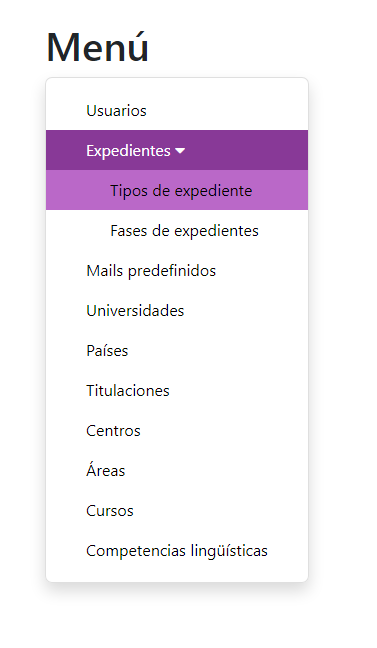
\includegraphics[height=0.4\textheight]{img/Capturas de twinX/sidebar_panel}
	\caption{Menú lateral del panel en twinX}
	\label{fig:sidebarpaneltwinX}
\end{figure}

Para conseguir el funcionamiento de \textit{dropdown}, hemos escrito el siguiente código con jQuery (\texttt{backend/web/js/dropdown\_expediente\_panel.js}):

\begin{minted}[frame=lines,breaklines]{javascript}
	let submenusExpedientes = ['tipo-expediente', 'fase-expediente', 'envio-mail-fase'];
	$(document).ready(function() {
		submenusExpedientes.forEach(function (str) {
			if (window.location.pathname.includes(str))
			toggleCollapse();
		});
	});
\end{minted}

Tras la creación del menú CRUD de los usuarios (el modelo ya está creado con anterioridad con la migración), se crean, por un lado, la clase de controlador, \texttt{UserController.php}, dentro de \texttt{backend/modules/panel/controllers}. Un nivel más arriba, en \texttt{views}, se tiene una nueva carpeta llama \texttt{user}, que posee los siguientes archivos:

\begin{itemize}
	\item \textbf{\texttt{\_form.php}}: es el formulario (\texttt{ActiveForm} de Yii, que renderiza un elemento \texttt{form} de HTML) que es utilizado por las vistas que necesiten cargar el formulario de datos de un usuario en la base de datos.
	\item \textbf{\texttt{create.php}}: es el receptor de la acción \texttt{create} del controlador, el cual renderiza el formulario \texttt{\_form.php} para crear un usuario nuevo.
	\item \textbf{\texttt{update.php}}: también carga el mismo formulario, pero recibe la acción \texttt{update} del controlador, el cual envía la información que ya se tiene sobre un usuario en concreto.
	\item \textbf{\texttt{view.php}}: la vista de los datos del usuario en detalle.
\end{itemize}

Cada uno de estos archivos conforma la vista de un componente; en este caso, el de usuario.

Sobre los controladores, diremos que son los orquestadores de lo que se ve en pantalla, hasta el punto de que, de alguna manera, al escribir en la barra de direcciones \texttt{localhost/panel/user/view?id=3}, lo que ocurre es que se llama al método \texttt{actionView} de la clase \texttt{UserController}. Es decir, se llama al método \texttt{actionX} de la clase \texttt{yController}, donde claramente «x» es \texttt{view} en nuestro caso e «y», \texttt{User}. Con esto, y tras la atenta visualización de la ausencia, como se podría esperar, de un archivo \texttt{delete.php} en la vista, podemos imaginar que al ir a \texttt{localhost/panel/user/delete?\\id=3} se ejecutará el método \texttt{actionDelete}, que al igual que \texttt{actionView} acepta el parámetro \texttt{\$id}. Pensemos, pues, que para eliminar un registro no necesitamos ninguna vista, pero sí un método en el controlador. Al fin y al cabo, ese método ordenará al modelo eliminar el registro, que es lo único que necesitábamos.

Los modelos son clases más sencillas, las cuales tienen la especificación de los atributos que tiene la tabla en concreto en base de datos, los métodos para recuperar los objetos de otros modelos a los que referencian (por ejemplo, como hemos dicho antes, una universidad pertenece a un país y, por tanto, el objeto del modelo de \texttt{Pais} estará dentro de \texttt{Universidad}), y otros métodos que generalmente creemos nosotros para acceder a datos externos de manera más rápida.

Una vez hemos hecho un recorrido por los tres grandes tipos de clases que tenemos, modelos, vistas y controladores, podemos entonces comprender el significado de nuestro patrón arquitectónico, el significado y la influencia que tiene en twinX y lo coherente que es el establecer esta separación.

Volviendo al desarrollo, tras crear con Gii la tabla CRUD (figura \ref{fig:giicruduser}), el resultado es el menú de la figura \ref{fig:usuariostwinX}. Normalmente, las tablas CRUD suelen tener un botón verde que permiten crear un nuevo registro, pero en el caso de los usuarios, se ha eliminado, ya que al crearlo manualmente desde este menú, no se genera un hash para la contraseña, al mismo tiempo que tampoco tiene gran relevancia el poder crear usuarios desde el panel de control, cuando el principal interés está puesto en gestionar los permisos de los integrantes de la comunidad.

\begin{figure}
	\centering
	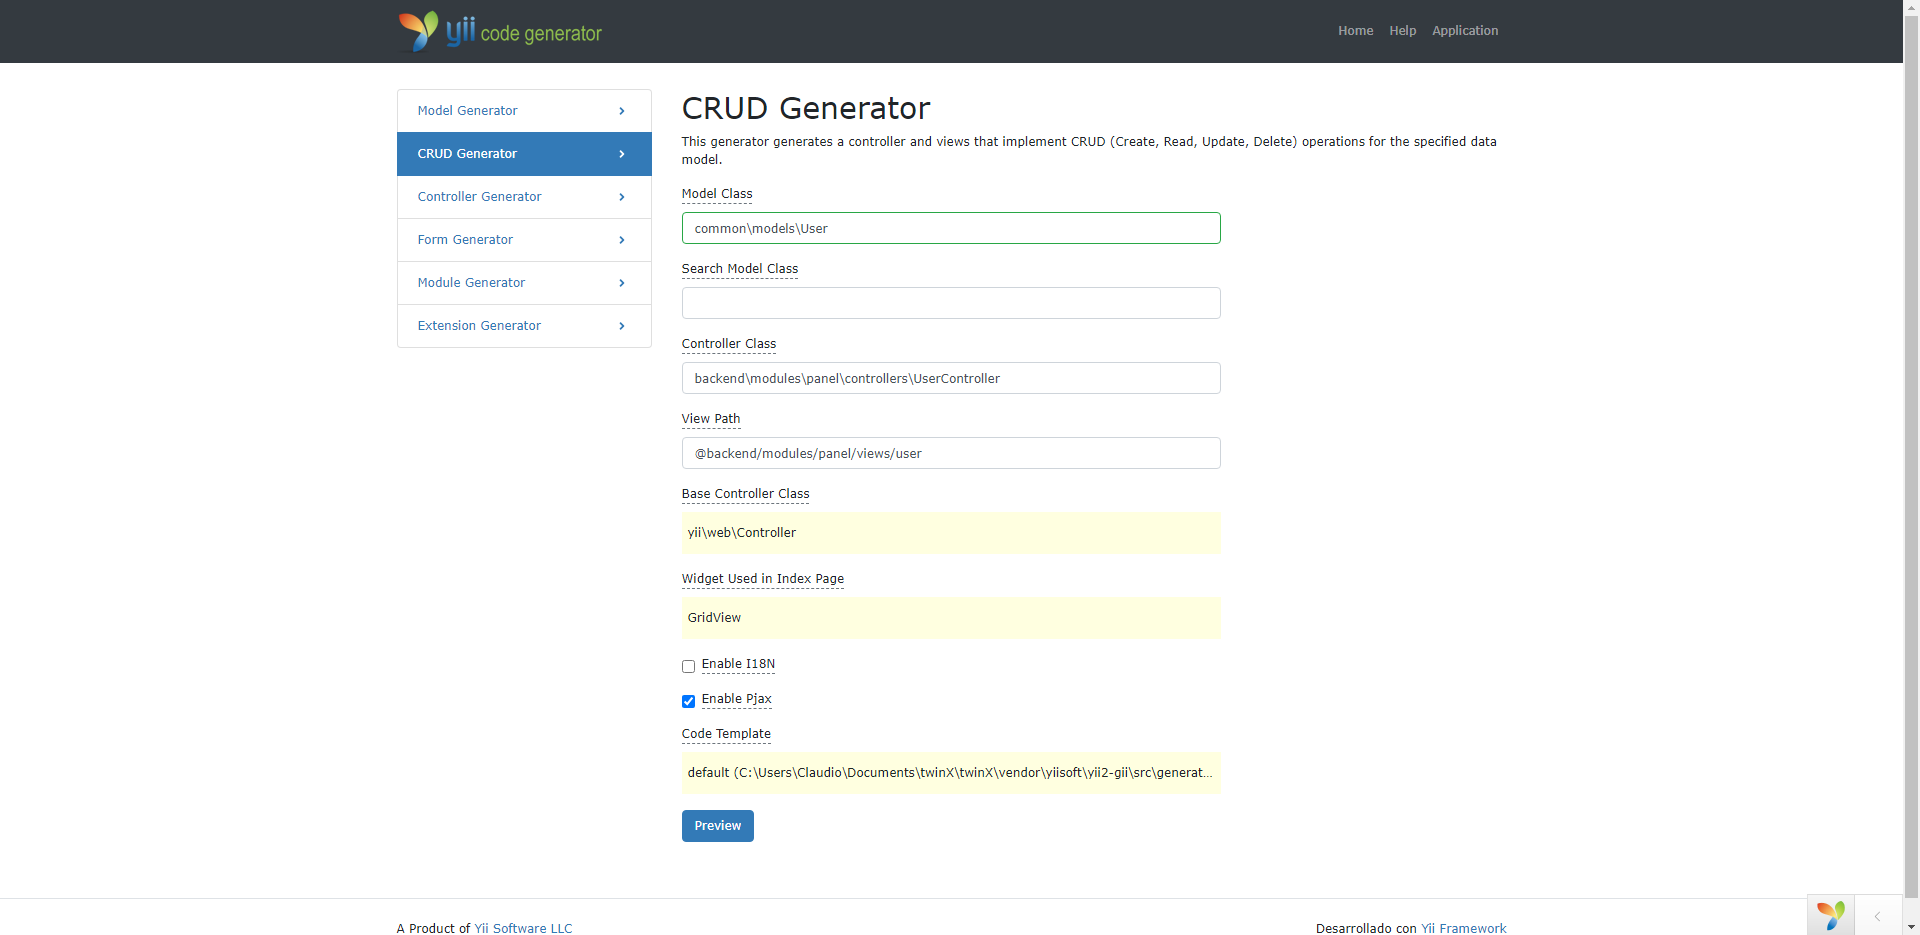
\includegraphics[width=\textwidth]{img/Capturas de twinX/gii_crud_user}
	\caption{Generación de la tabla CRUD de User}
	\label{fig:giicruduser}
\end{figure}


\begin{figure}
	\centering
	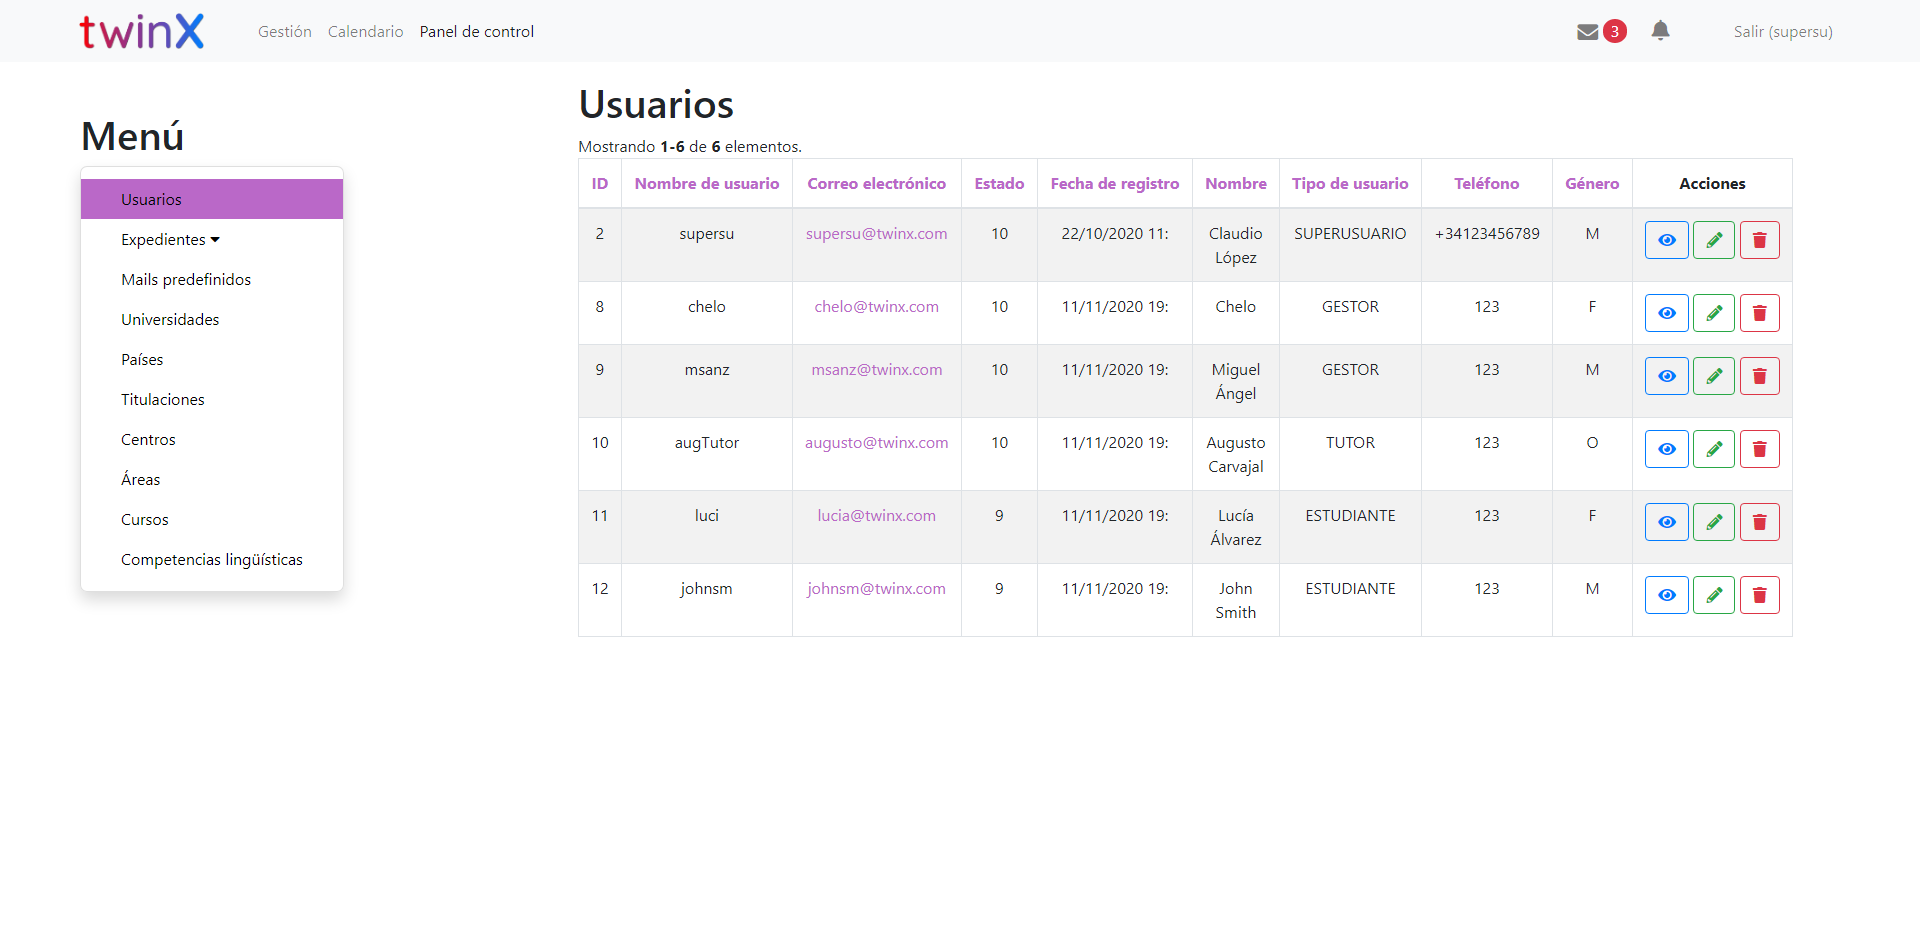
\includegraphics[width=\textwidth]{img/Capturas de twinX/usuarios_twinX}
	\caption{Menú de usuarios en twinX}
	\label{fig:usuariostwinX}
\end{figure}

Como ya hemos señalado con anterioridad, se tomó la decisión de mantener las vistas de los registros almacenados sin apenas modificar en este módulo de panel de control. Por defecto, lo que podemos ver en la interfaz de vista de un registro es lo que encontramos en la figura \ref{fig:vistatitulaciontwinX}.

\begin{figure}
	\centering
	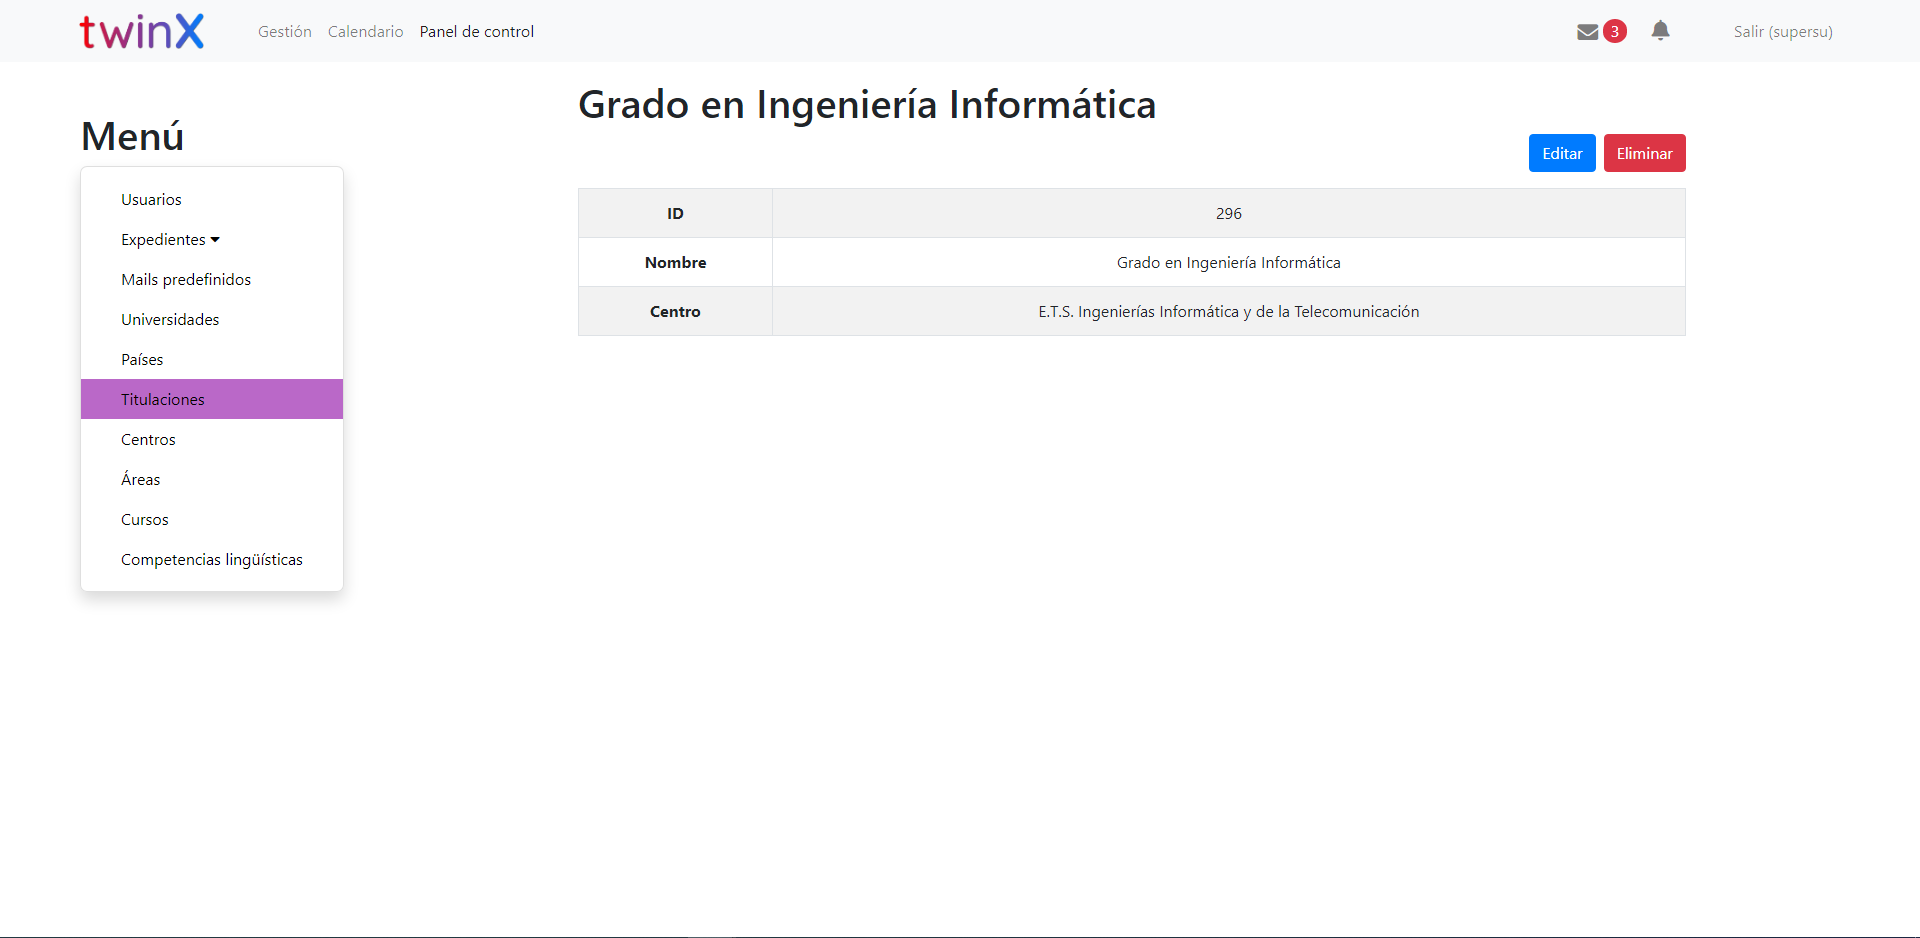
\includegraphics[width=\textwidth]{img/Capturas de twinX/vista_titulacion}
	\caption[Vista de un registro en twinX]{Vista de un registro en twinX (menú de titulaciones)}
	\label{fig:vistatitulaciontwinX}
\end{figure}

Por defecto, Gii pone los botones justo a la izquierda de las cabeceras de las tablas y de las vistas. Sin embargo, hemos tomado la decisión de modificar esto, como se puede apreciar en la figura \ref{fig:vistatitulaciontwinX}, donde los botones de «editar» y «eliminar» están a la derecha. El motivo es porque mayormente en las tablas del menú \texttt{index} de cada categoría, como la de la figura \ref{fig:fasesexpedientesindex} se podía ver un exceso de información de haber dejado el botón en la izquierda, pues tendríamos el título, el indicador del total de elementos de la tabla y el botón. Por tanto, hemos dejado todos los botones a la izquierda en las sucesivas vistas de los menús de toda la plataforma. Por supuesto, no hemos hecho los cambios de forma manual, sino que se ha modificado el código del generador de Gii para que todas las genere automáticamente como describimos. Esto es posible modificando el archivo \texttt{index.php} para la tabla del menú y el \texttt{view.php} para la vista de un registro en el directorio \texttt{vendor/yiisoft/yii2-gii/src/generators/crud/default/views}\footnote{Este directorio no se encuentra en el respositorio de GitHub \cite{repogit}, dado que forma parte de los archivos del motor de Yii y se encuentran dentro del archivo \texttt{.gitignore}, por lo que no se guardan, dado que pueden obtenerse clonando el repositorio de Yii \cite{yii2advanced}}. Sobre el primero de los archivos, diremos que también hemos hecho las pertinentes modificaciones para que cada una de las vistas tenga el botón del ojo (acceso a la vista en detalle) el lápiz (para editar la entrada) y la papelera (para la eliminación) para interaccionar con cada registro en concreto.

\begin{figure}
	\centering
	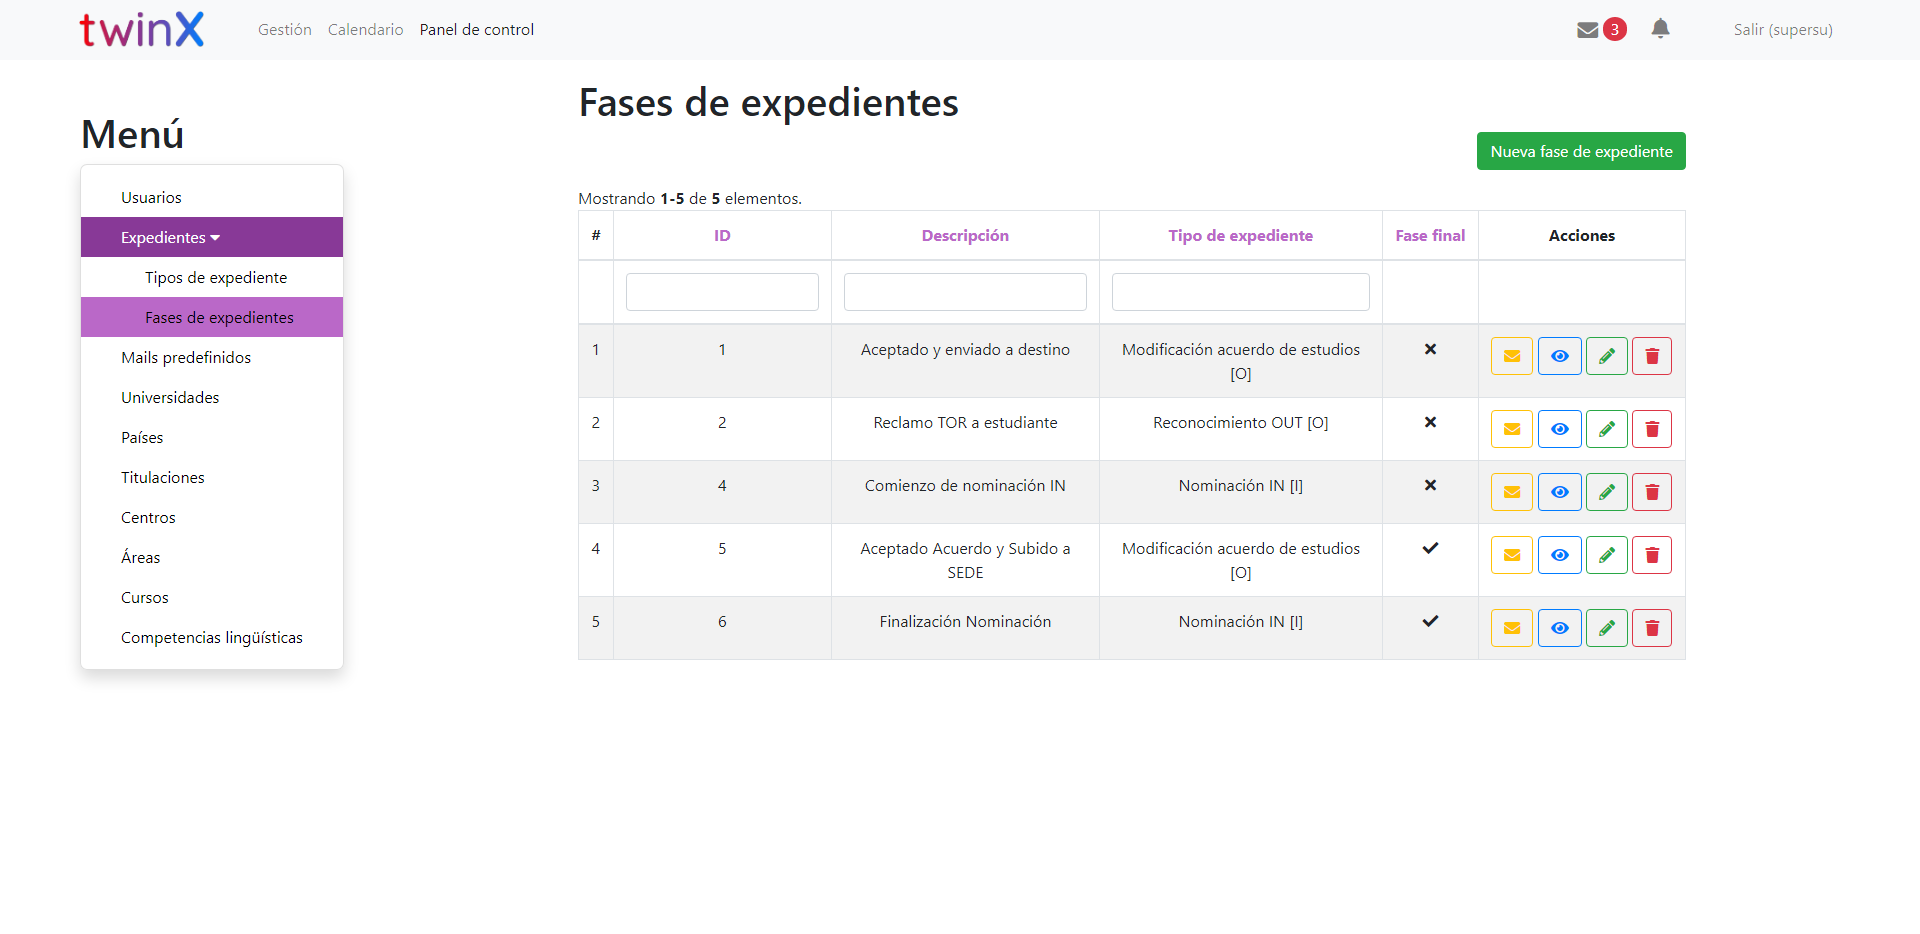
\includegraphics[width=\textwidth]{img/Capturas de twinX/fases_expedientes_index}
	\caption{Menú de fases de expedientes en twinX}
	\label{fig:fasesexpedientesindex}
\end{figure}

Por último, vamos a destacar la vista de una fase de expediente. Recordemos que el procesar una fase implicaba enviar varios correos a responsables y a destinatarios relacionados con la situación del estudiante (o incluso a él mismo). Por tanto, hemos incluido en la vista de las fases, los mensajes que se enviarían tras procesarla (figura \ref{fig:fasesexpedientesvista}). También podemos verlos pulsando en el botón amarillo con el sobre de la figura \ref{fig:fasesexpedientesindex}, donde se dan aún más opciones al usuario. La implementación de esta parte no es compleja pero sí tediosa, por lo que vamos a omitir su explicación por el momento, dado que en la próxima sección veremos otro ejemplo, ya que en el módulo de gestión \ref{sec:gestion} hemos diseñado una vista compuesta de forma similar.

\begin{figure}
	\centering
	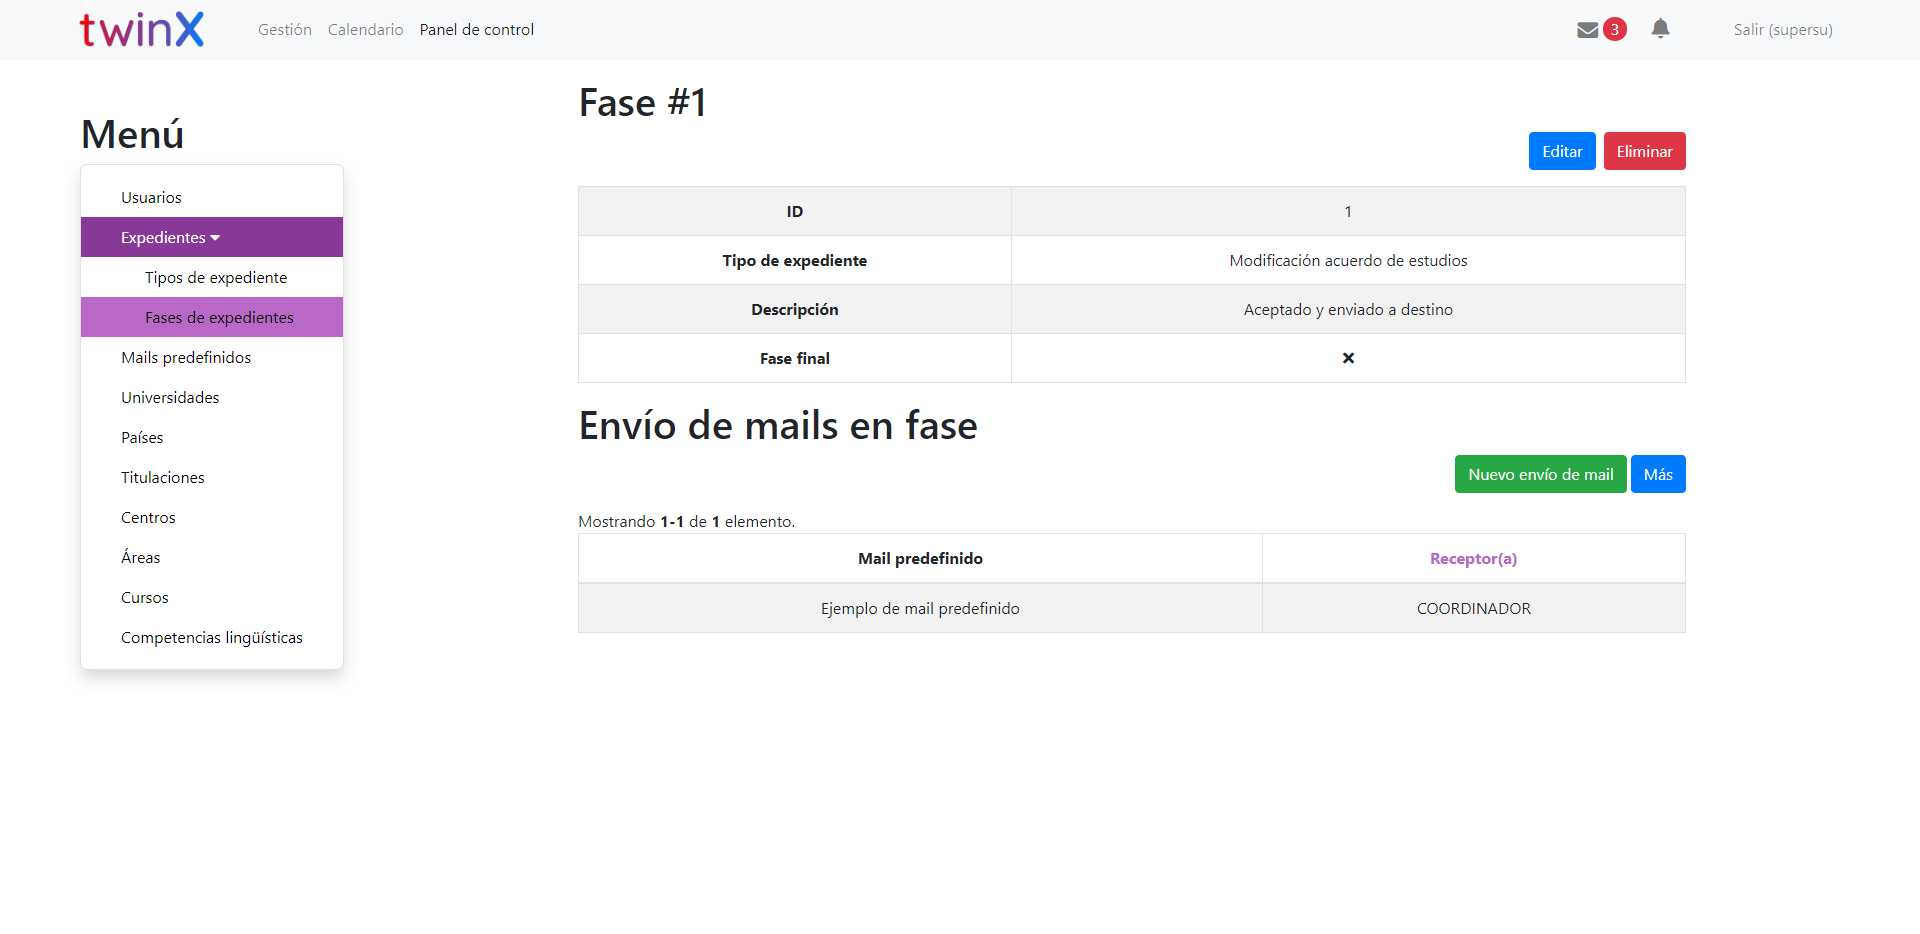
\includegraphics[width=\textwidth]{img/Capturas de twinX/fases_expedientes_vista}
	\caption{Vista de una fase de expediente en twinX}
	\label{fig:fasesexpedientesvista}
\end{figure}



\section{Desarrollo del módulo de gestión}
\label{sec:gestion}

Para desarrollar esta parte de la aplicación, también se ha creado un módulo y las tablas CRUD pertinentes para cada una de las secciones de Gestión. Recordamos que es el corazón de la aplicación, donde los gestores acudirían diariamente a desempeñar su trabajo: consulta de la información referente a un estudiante, tramitación de algún expediente, cambios en su acuerdo de estudios, etc.

\subsection{Integración del menú de convenios}

Uno de los mayores desafíos ha sido, como era de imaginar a la hora de ver el modelo de la base de datos (figura \ref{fig:modeloBD}), el diseñar un formulario para los convenios recogido y no puesto tal cual sale de Gii. Para ello hemos empleado el objeto de Bootstrap \texttt{card} y \texttt{accordion}. Conforme vamos desplegando cada una de las secciones, las otras se cierran para no ocupar espacio en la pantalla y hacer que el usuario se centre en la introducción de los datos en una sección concreta. También hemos usado tarjetas a distintos niveles para estructurar los formularios de la mejor manera posible (figuras \ref{fig:creacionconvenio1} y \ref{fig:creacionconvenio2})

\begin{figure}
	\centering
	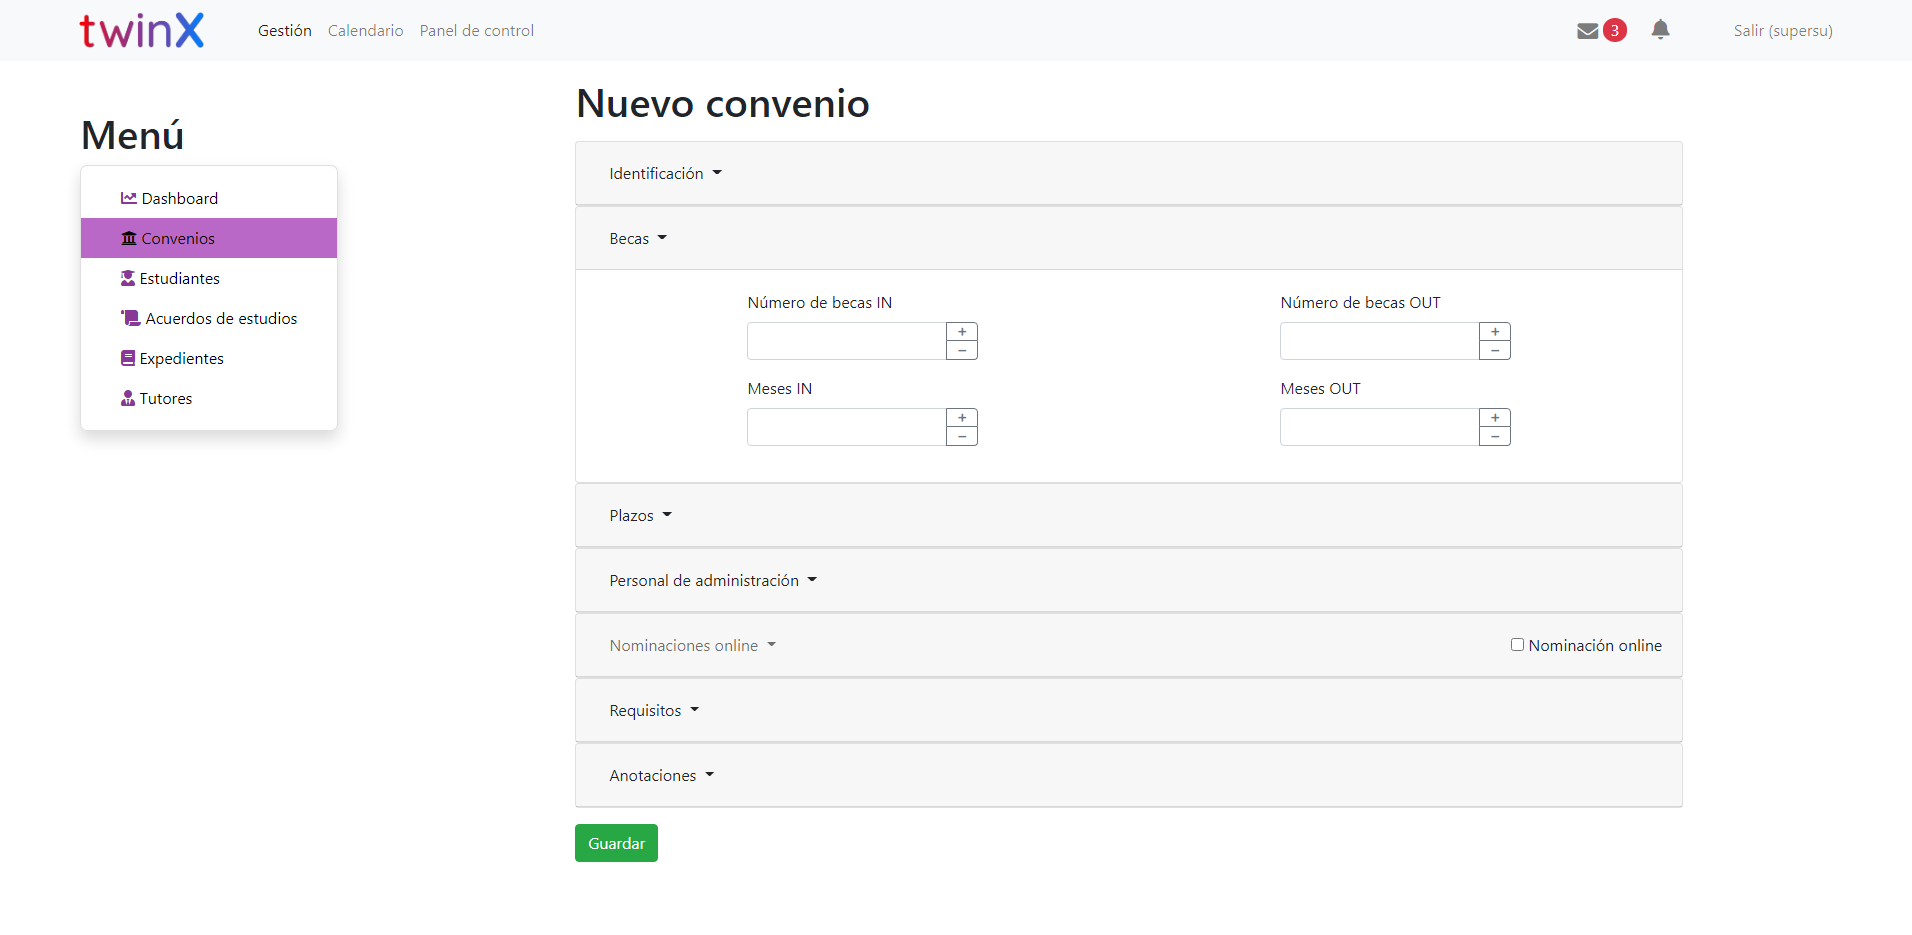
\includegraphics[width=\textwidth]{img/Capturas de twinX/creacion_convenio_1}
	\caption{Creación de un convenio en twinX}
	\label{fig:creacionconvenio1}
\end{figure}

\begin{figure}
	\centering
	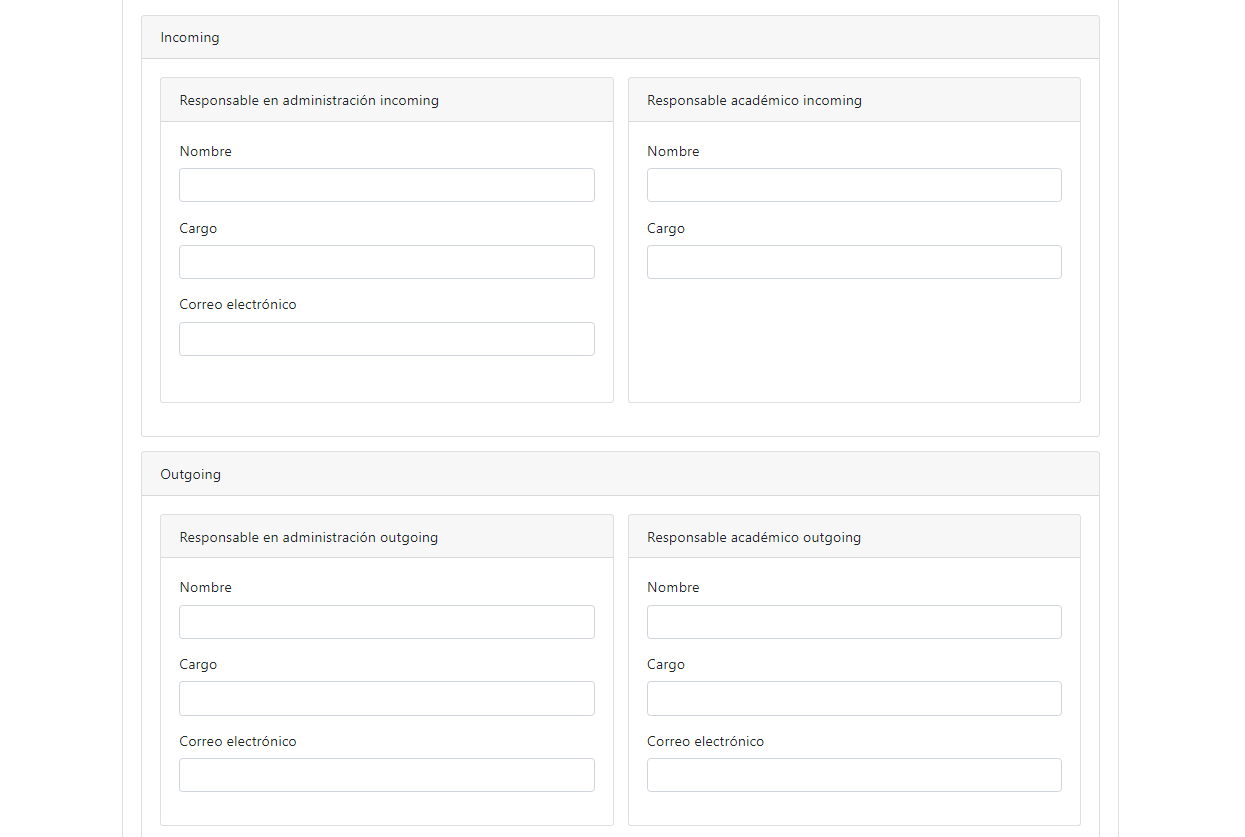
\includegraphics[width=\textwidth]{img/Capturas de twinX/creacion_convenio_2}
	\caption[Creación de un convenio en twinX 2]{Creación de un convenio en twinX: introducción de datos de los responsables externos}
	\label{fig:creacionconvenio2}
\end{figure}

Por defecto, Gii espera que en campos donde en la tabla se tiene una restricción de clave externa se introduzca, mediante un campo de texto libre, un identificador, por ejemplo, del país del convenio. Sin embargo, esta es una de los numerosos cambios que se comienzan haciendo al recibir el código generado: adaptarlo al usuario. Para ello y durante todo el proyecto en general, hemos hecho uso de librerías del autor \textit{Kartik} \cite{krajee} y como resultado, tenemos elementos que ya están disponibles en Yii2 como es la inserción de un menú \textit{dropdown} para escoger entre varias opciones, pero potenciado con una búsqueda, por ejemplo, como se aprecia en la figura \ref{fig:creacionconvenio3}. Pensemos que elementos como este son indispensables, pues en el uso cotidiano, twinX almacenaría cientos de estudiantes, decenas de universidades y convenios tal y como hace TWINS hasta el momento; por tanto, la opción de un desplegable estático no funcionaría en este contexto. Su uso es verdaderamente sencillo, una vez que nos familiarizamos con la sintaxis:

\begin{minted}[frame=lines]{php}
	<?php
	(...)	
	 <?= $form->field($model, 'cod_pais')->widget(Select2::className(), [
		'data' => ArrayHelper::map(Pais::find()->all(), 'iso', 'nombreISO'),
		'theme' => Select2::THEME_KRAJEE_BS4,
		'options' => [
			'placeholder' => 'Seleccione un país',
		]
	]) ?>
	
\end{minted}


\begin{figure}
	\centering
	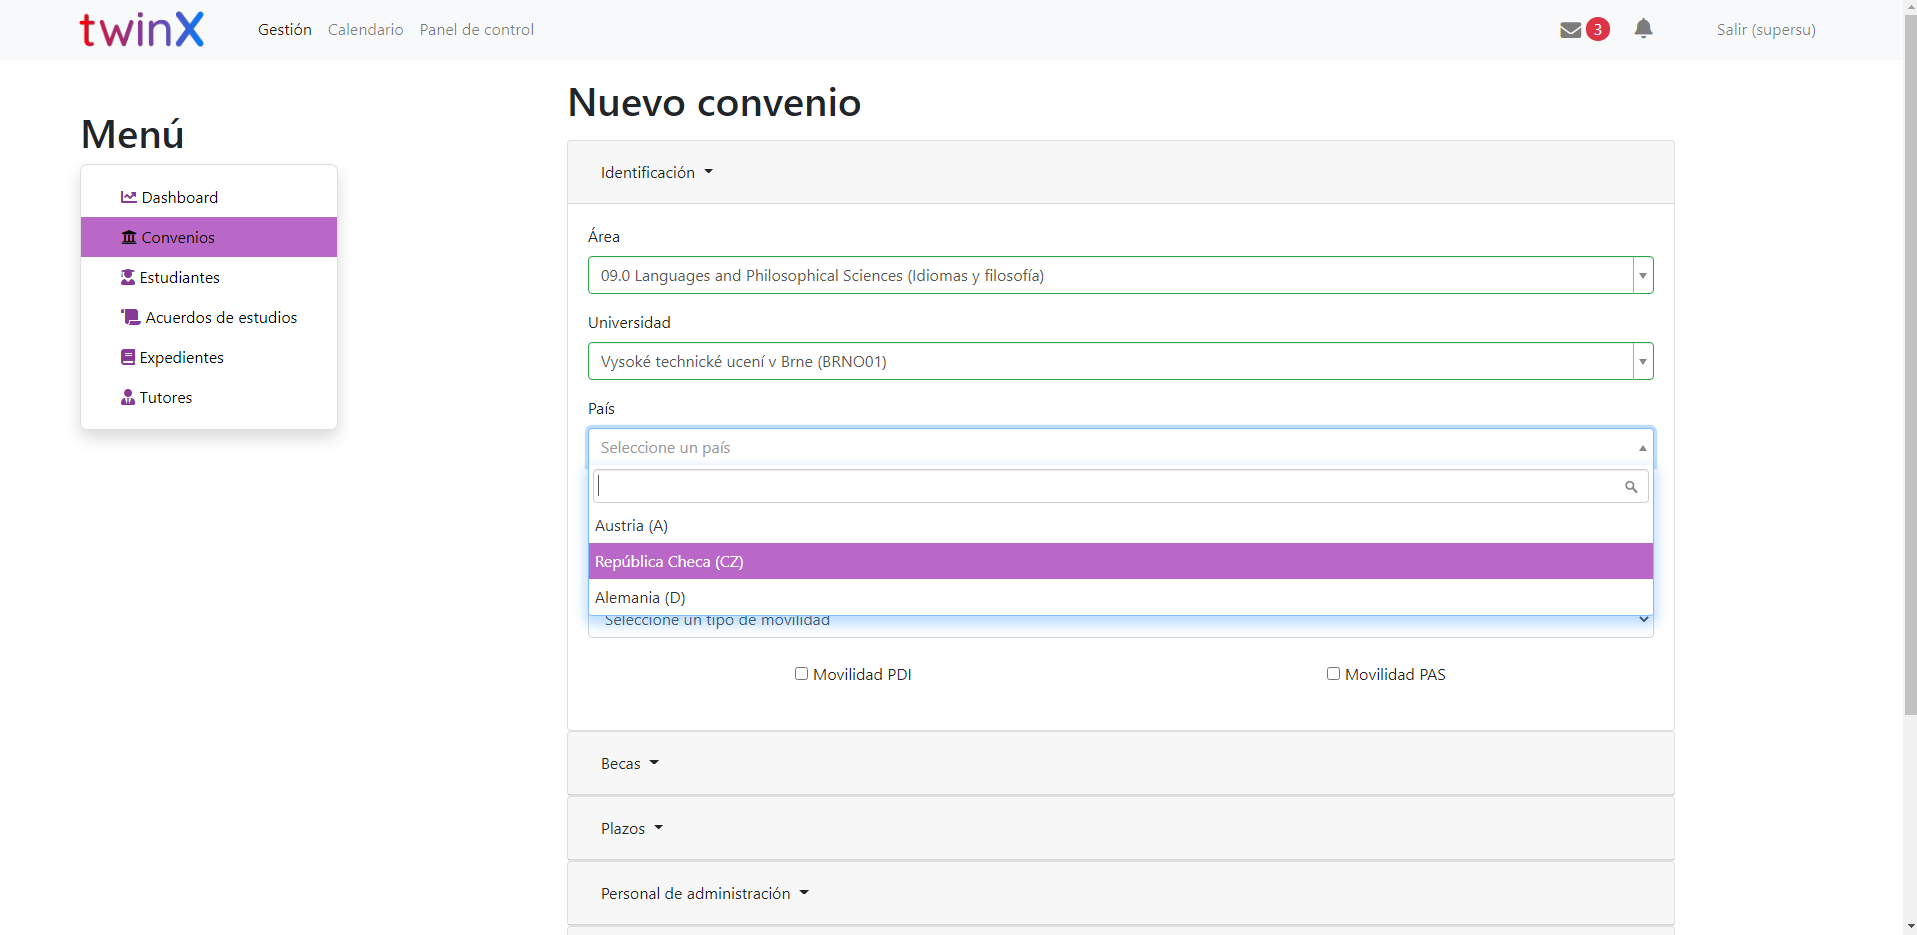
\includegraphics[width=\linewidth]{img/Capturas de twinX/creacion_convenio_3}
	\caption[Creación de un convenio en twinX 3]{Creación de un convenio en twinX: introducción de datos externos al modelo \texttt{Convenio}}
	\label{fig:creacionconvenio3}
\end{figure}

Otra dificultad de la implementación del formulario de los convenios estaba en la selección de los requisitos lingüísticos. Éstos se almacenan en una tabla aparte, pero existe una relación muchos a muchos que relaciona un convenio con varias competencias o la pertenencia de una sola competencia a muchos convenios. El problema estaba cuando queríamos asociar un par \texttt{(id\_convenio, id\_requisito)} sin tener de antemano la ID del convenio que se está creando. Para ello ha sido necesario crear una \textbf{transacción}. Es decir, primeramente tenemos que asegurarnos de que guardamos todos los datos del convenio. Acto seguido, asociar los requisitos lingüísticos que se han escogido para el convenio a crear y, después, guardar los cambios. Si alguna de estas acciones no prospera, tendremos que cancelar todo y devolver la tabla a su estado anterior. Esto podemos conseguirlo sobrecargando el método de guardado, \texttt{save}.
Es más, también hemos de tener en cuenta que el tratamiento de los requisitos puede darse en la edición del convenio, con lo cual, puede haber requisitos ya en la tabla que tenemos que recuperar, y a la hora de ejecutar la transacción, evaluar cuáles estaban ya en la tabla de la relación convenio - requisito y dejarlos intactos, cuáles han de ser eliminados y cuáles insertados como nuevos registros.
Para ello, tenemos que crear una nueva clase \texttt{ConvenioForm} que e\texttt{Convenio} (modelo) y herede sus métodos. Entonces, programamos toda esta funcionalidad que hemos descrito y solo cuando sea necesario, hacemos la llamada a este nuevo modelo. Una de las características más novedosas es la sobrecarga del método \texttt{afterFind}, que ejecuta justo después de buscar la recuperación de los requisitos actuales del convenio (si los tiene). Gracias a ello, podemos trabajar con un array de requisitos y ejecutar las acciones descritas:

\begin{minted}[frame=lines]{php}
<?php
(...)

class ConvenioForm extends Convenio
{
	public $requisitos = [];
	private $_requisitos;
	
	public function save($runValidation = true, $attributeNames = null)
	{
		$transaction = \Yii::$app->db->beginTransaction();
		
		try {
			if (!parent::save($runValidation, $attributeNames)) {
				return false;
			}
			
			$this->addNewRequisitos();
			$this->deleteOldRequisitos();
			
			$transaction->commit();
			
		}
		
		catch (Exception $e) {
			$transaction->rollBack();
			
			throw $e;
		}
		
		return true;
	}
	
	protected function addNewRequisitos()
	{
		$nuevos = [];
		
		if ($this->isNewRecord) {
			$nuevos = $this->requisitos;
		}
		else if(!empty($this->requisitos)){
			foreach ($this->requisitos as $requisito) {
				if (!in_array($requisito, $this->_requisitos)) {
					$nuevos[] = $requisito;
				}
			}
		}
		
		if(!empty($nuevos)) {
			foreach ($nuevos as $requisito) {
				$relacion = new ReqLingConv();
				
				$relacion->id_conv = $this->id;
				$relacion->id_comp = $requisito;
				
				if (!$relacion->save()) {
					throw new Exception('Error al guardar el requisito lingüístico');
				}
			}
		}
	}
	
	protected function deleteOldRequisitos()
	{
		foreach ($this->reqLingConvs as $requisito) {
			if (!in_array($requisito->id, $this->requisitos) && $requisito->delete() === false) {
				throw new Exception('Failed to save related records.');
			}
		}
	}
	
	public function afterFind()
	{
		foreach ($this->reqLingConvs as $requisito) {
			$this->requisitos[] = $requisito->id;
		}
		
		$this->_requisitos = $this->requisitos;
		
		parent::afterFind();
		
	}
}
\end{minted}

El proceso llevado a cabo en \texttt{EstudianteForm} es muy similar, dado que también necesitamos, en el formulario de un estudiante, especificar las competencias lingüísticas que posee.

En el menú de convenios (figura \ref{fig:menuconveniotwinX}) hemos tenido que cambiar bastantes cosas. Para ello, ha sido necesario crear bastantes métodos en el modelo de Convenio. Por ejemplo, para obtener el ratio de estudiantes nominados del total de estudiantes que contiene el convenio. O los convenios con su código completo (código ISO del país, código de la universidad y área de conocimiento según el ISCED\footnote{International Standard Classification of Education}). Del mismo modo, hemos tenido que ajustar la visualización de los nombres de la universidad o del área completos, ya que la generación de código automática solo mostraba los ID en la base de datos:

\begin{minted}[frame=lines]{php}
<?php
(...)
<?= GridView::widget([
	'dataProvider' => $dataProvider,
	'filterModel' => $searchModel,
	'columns' => [
	
		[
			'attribute' => 'numAcuerdos',
			'label' => 'Nº de acuerdos'
		],
		[
			'attribute' => 'nominadosAcuerdos',
			'label' => 'Nominados totales',
			'format' => 'raw'
		],
		[
			'attribute' => 'codConvenio',
			'label' => 'Convenio',
			'format' => 'raw',
		],
		[
			'attribute' => 'nombreCodUni',
			'label' => 'Universidad'
		],
		[
			'attribute' => 'areaCompleta',
			'label' => 'Nombre de la área'
		],
	
	
		'tipo_movilidad',
	
		[
		'class' => 'yii\grid\ActionColumn',
			'template' => '{view}',
			'header' => 'Acciones'
		],
	],
]); ?>
\end{minted}

\begin{figure}
	\centering
	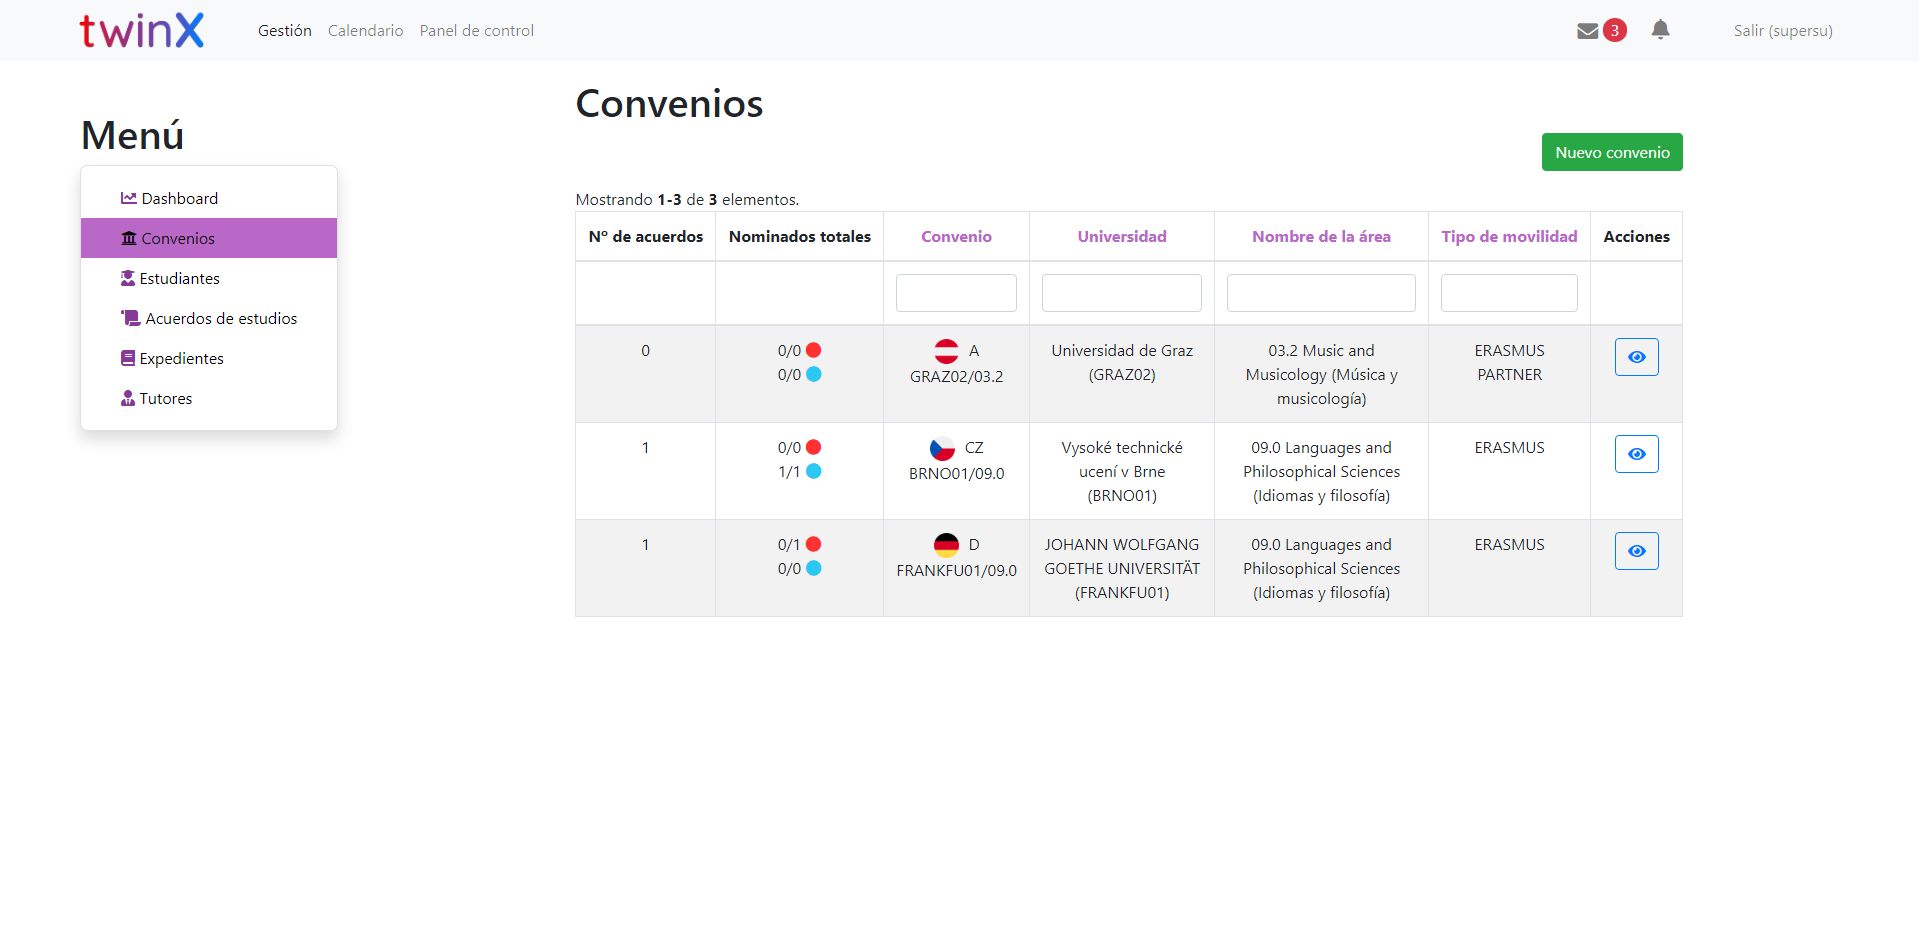
\includegraphics[width=\linewidth]{img/Capturas de twinX/menu_convenio}
	\caption{Menú de convenios en twinX}
	\label{fig:menuconveniotwinX}
\end{figure}

Todos los atributos que vemos en el código son generados por métodos creados en el modelo:

\begin{minted}[frame=lines]{php}
<?php
(...)
public function getNombreCodUni()
{
	return $this->codUni->getNombreCodigo();
}

public function getAreaCompleta()
{
	return $this->codArea->getAreaCompleta();
}
\end{minted}

También podríamos haber hecho ese acceso desde la vista, pero aunque no es una buena práctica, nos complicaría mucho las cosas. El tener los atributos definidos en el modelo, nos permite acceder a ellos desde una clase especial de la que aún no hemos hablado. Son las clases de búsqueda, y se encuentran en \texttt{common/models/search}, nombradas como \texttt{ConvenioSearch} en caso del convenio. Es ahí donde tenemos que decir qué atributos propios hemos definido en nuestro modelo, para poder unir las tablas a las que refieren y así poder hacer tanto búsquedas como ordenaciones, introduciendo términos en los campos de texto de debajo de la cabecera de la tabla y haciendo click en los nombres de los atributos respectivamente. Para conseguir este comportamiento, ha sido necesario hacer en primer lugar, los atributos seguros (\textit{safe}):

\begin{minted}[frame=lines]{php}
<?php
(...)
class ConvenioSearch extends Convenio
{
	public $codConvenio, $nombreCodUni, $areaCompleta;
	
	/**
	* {@inheritdoc}
	*/
	public function rules()
	{
		return [
		(...)
		[['codConvenio', 'nombreCodUni', 'areaCompleta'], 'safe'],
		];
	}
	
	(...)
}
\end{minted}

Después, hacer la unión de la tabla con las demás y configurar las ordenaciones:

\begin{minted}[frame=lines]{php}
<?php
(...)
public function search($params)
{
	$query = Convenio::find();
	
	///
	$query->joinWith(['codPais', 'codArea', 'codUni']);
	
	// add conditions that should always apply here
	
	$dataProvider = new ActiveDataProvider([
	'query' => $query,
	]);
	
	///
	$dataProvider->sort->attributes['codConvenio'] = [
	'asc' => ['pais.iso' => SORT_ASC],
	'desc' => ['pais.iso' => SORT_DESC],
	'default' => SORT_DESC
	];
	
	$dataProvider->sort->attributes['nombreCodUni'] = [
	'asc' => ['universidad.nombre' => SORT_ASC],
	'desc' => ['universidad.nombre' => SORT_DESC],
	'default' => SORT_DESC
	];
	
	$dataProvider->sort->attributes['areaCompleta'] = [
	'asc' => ['area.cod_isced' => SORT_ASC],
	'desc' => ['area.cod_isced' => SORT_DESC],
	'default' => SORT_DESC
	];

	(...)
}

(...)

?>
\end{minted}

Y por último, añadir el filtrado a las búsquedas que se hagan introduciendo texto:

\begin{minted}[frame=lines]{php}
<?php
(...)

->andFilterWhere(['like', 'pais.iso', $this->codConvenio])
->orFilterWhere(['like', 'area.cod_isced', $this->codConvenio])
->orFilterWhere(['like', 'universidad.cod_uni', $this->codConvenio])
->andFilterWhere(['like', 'universidad.nombre', $this->nombreCodUni])
->orFilterWhere(['like', 'universidad.cod_uni', $this->nombreCodUni])
->andFilterWhere(['like', 'area.cod_isced', $this->areaCompleta])
->orFilterWhere(['like', 'area.nombre_isced', $this->areaCompleta])
->orFilterWhere(['like', 'area.nombre_area', $this->areaCompleta]);

(...)

?>
\end{minted}

Esto es extensible a todas las clases donde hemos usado atributos modificados y Yii no conoce la manera de aplicar los filtros, por lo que es obligatorio hacerlo cuando queremos ofrecer otra manera de comunicar la información distinta a la que ofrece el framework por defecto. En muchos casos esto se complica bastante. Por ejemplo, en la unión de las tablas:

\begin{minted}[frame=lines,breaklines]{php}
<?php
(...)

$query->joinWith(['ae.estudiante.usuario', 'ae.estudiante.convenio.codPais', 'tipoExp', 'relExpFases.fase', 'ae.estudiante.convenio.codArea']);

?>
\end{minted}

Este es el código de la clase \texttt{ExpedienteSearch.php}, dadas las numerosas referencias a otras clases externas a ella.

Una vez comentadas las vistas de creación, actualización y de menú principal, vamos a abordar la de vista (figura \ref{fig:vistaconveniotwinX}). Los datos se han separado en distintas secciones de nuevo, pero sin el comportamiento de acordeón que impedía abrir más de una sección al mismo tiempo. Para la vista se debe dar más libertad al usuario, y siempre puede contraer las secciones a su gusto; en cambio, para el formulario, es más importante forzar centrar su atención en una parte de los datos en concreto.

\begin{figure}
	\centering
	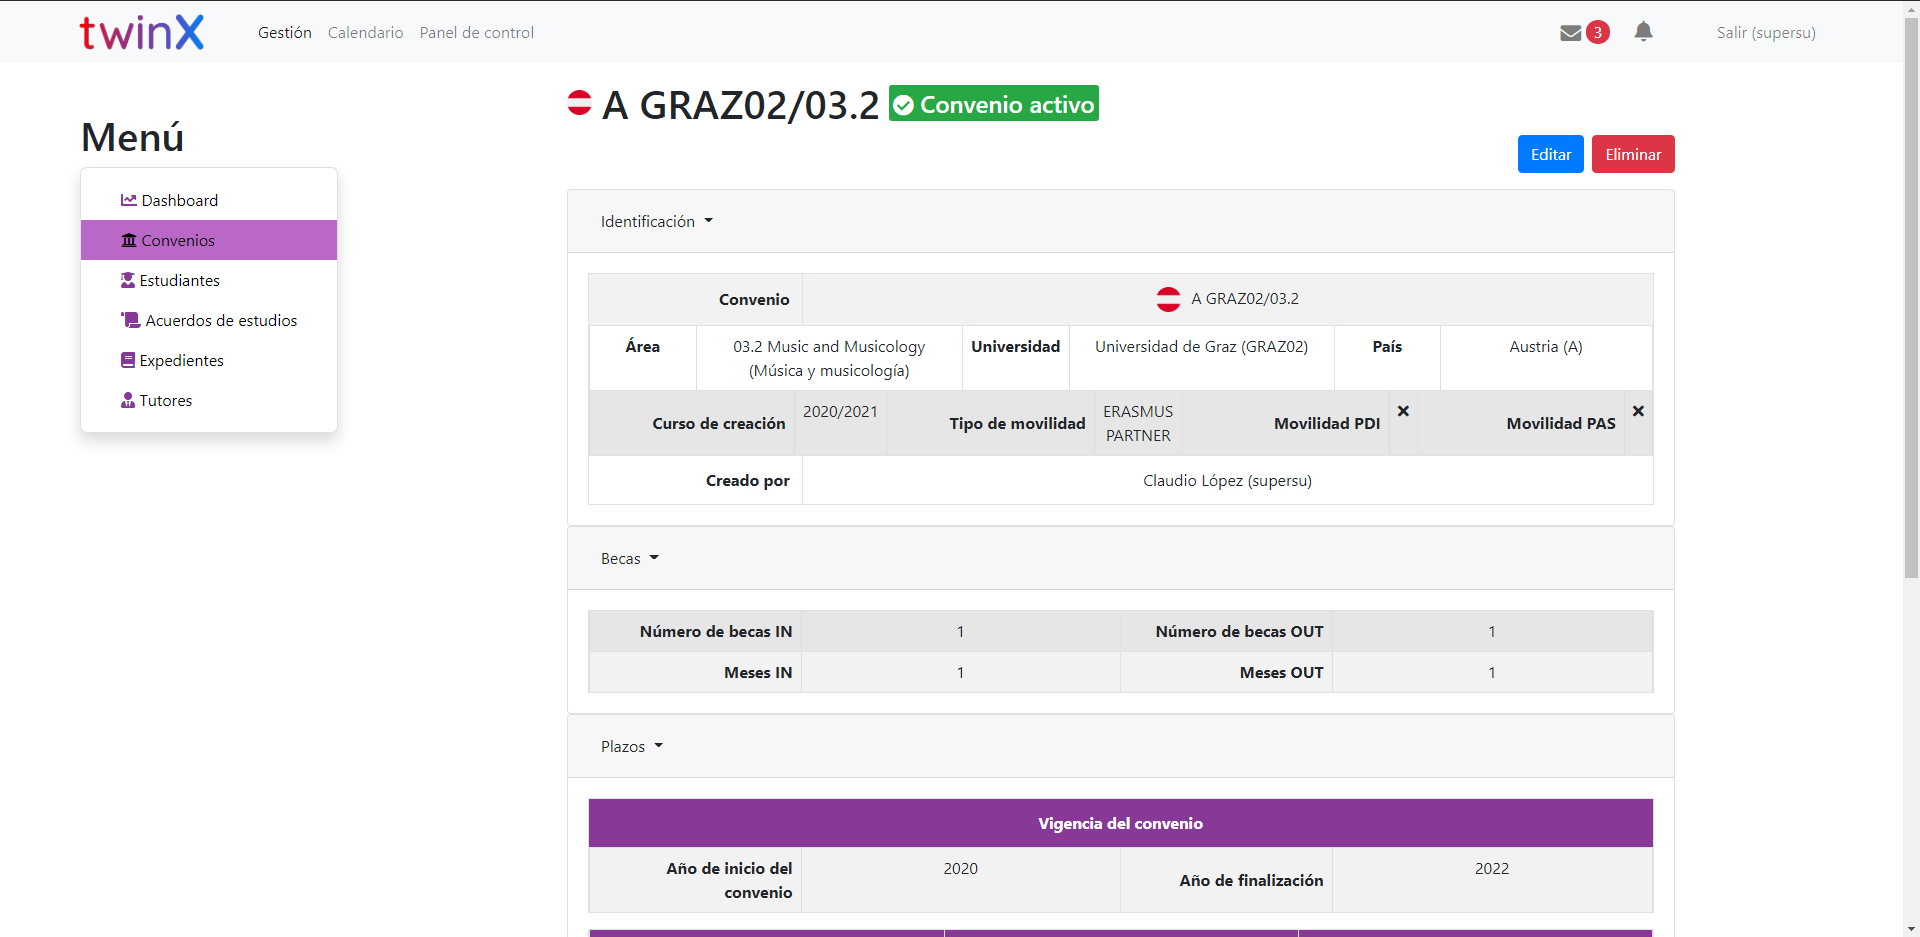
\includegraphics[width=\linewidth]{img/Capturas de twinX/vista_convenio}
	\caption{Vista de los convenios en twinX}
	\label{fig:vistaconveniotwinX}
\end{figure}


Destaca también el testigo de convenio activo, que indica si la fecha de vigencia del convenio es superior a la actual (convenio activo), si es inferior (inactivo) o si iguala al año (próxima caducidad)

\subsection{Integración del menú de estudiantes}

Respecto de los convenios, una de las cosas más destacable ya ha sido comentada: hemos necesitado ejecutar otra transacción para elegir las competencias lingüísticas de los estudiantes en su formulario (figura \ref{fig:formularioestudiantetwinX}) y para ello hemos creado una clase \texttt{EstudianteForm} que extiende a \texttt{Estudiante}.

\begin{figure}
	\centering
	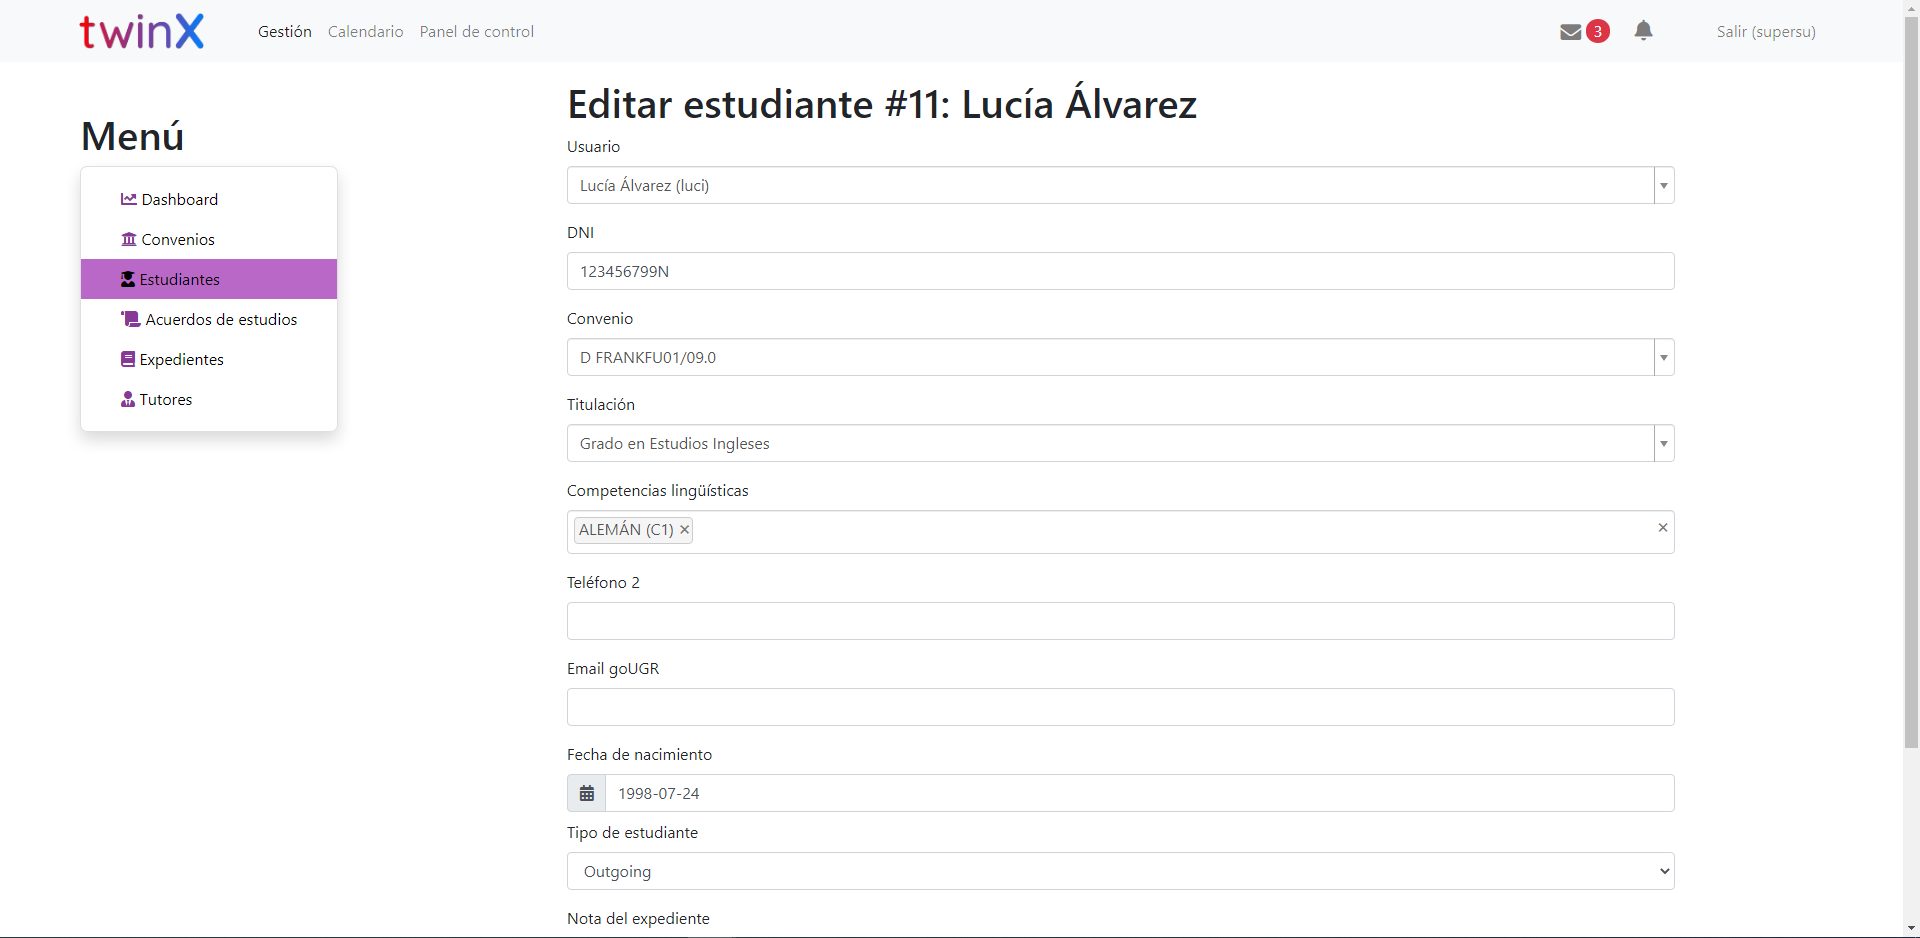
\includegraphics[width=\linewidth]{img/Capturas de twinX/formulario_estudiante}
	\caption{Creación de un estudiante en twinX}
	\label{fig:formularioestudiantetwinX}
\end{figure}

Desde el menú de estudiantes (figura \ref{fig:menuestudiantestwinX}) podemos pivotar hacia su convenio (icono verde) o hacia su acuerdo de estudios (icono turquesa). Al lado del nombre del estudiante, figura un círculo de color rojo o azul, según si es saliente o entrante, respectivamente, como apuesta de rediseño de rellenar el fondo del nombre del estudiante de uno de estos colores en TWINS según su modalidad (figura \ref{fig:alumnos}).

\begin{figure}
	\centering
	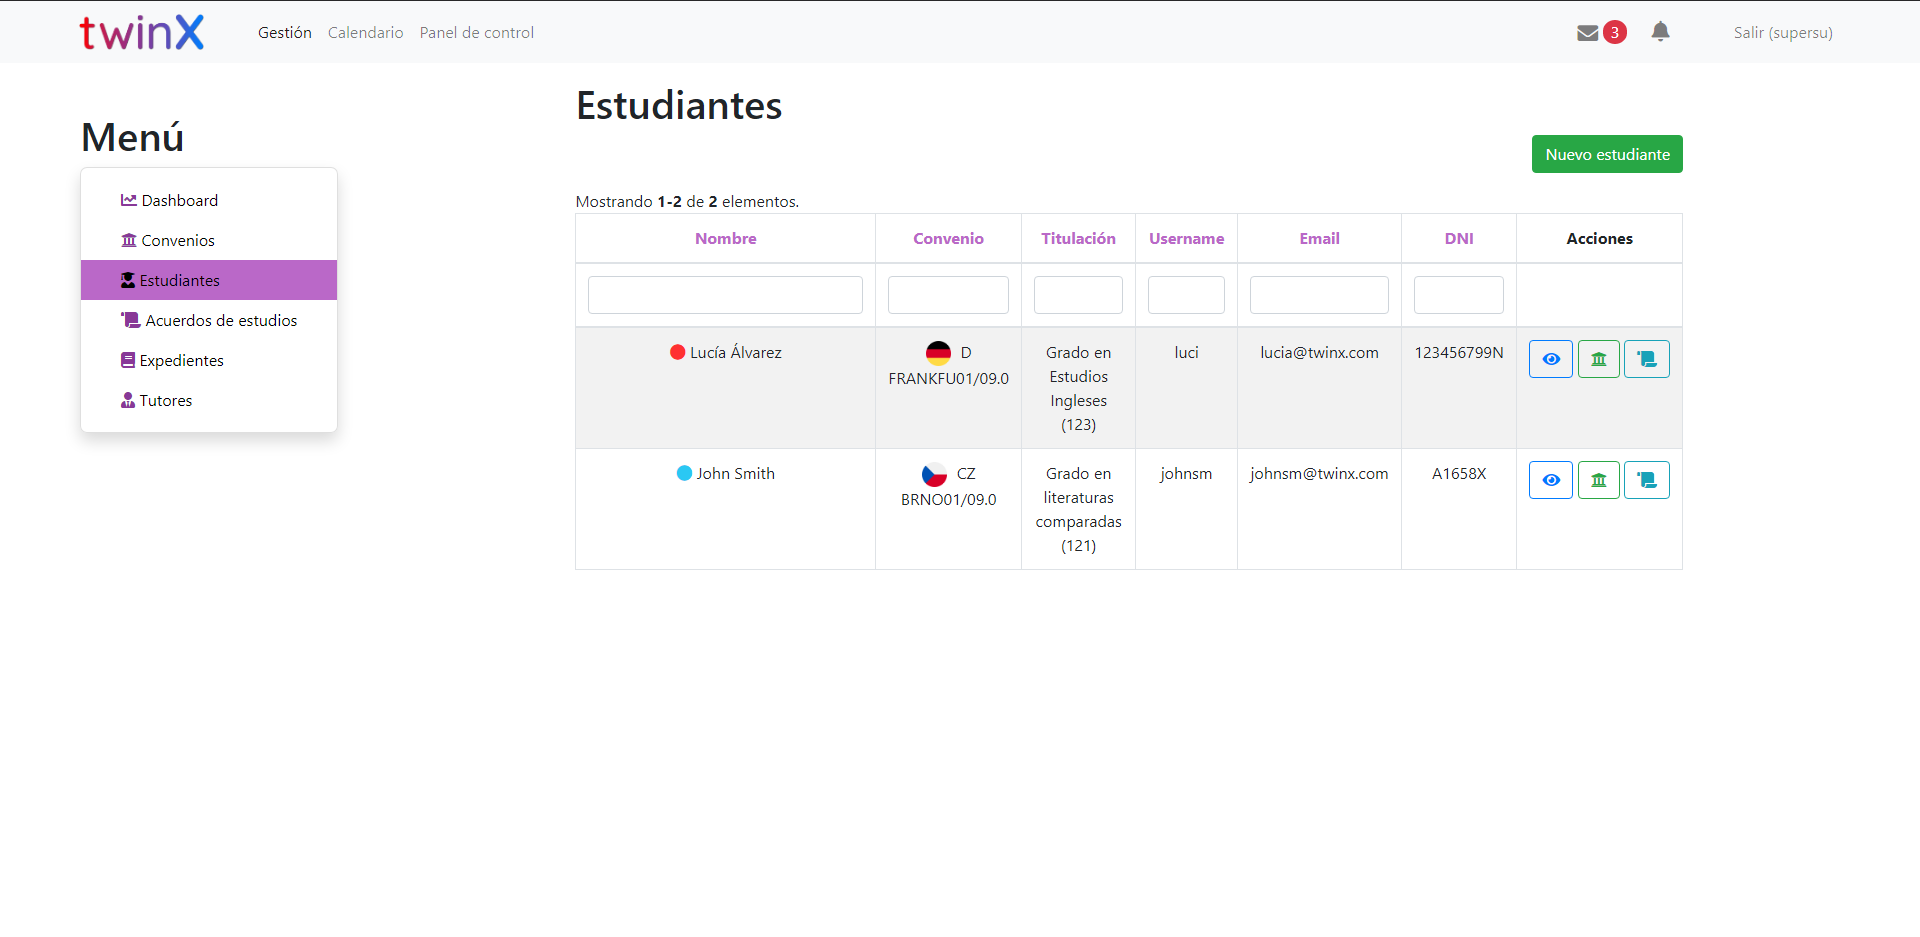
\includegraphics[width=\linewidth]{img/Capturas de twinX/menu_estudiante}
	\caption{Menú de estudiantes en twinX}
	\label{fig:menuestudiantestwinX}
\end{figure}

La vista del estudiante (\ref{fig:vistaestudiantetwinX}) también ha tenido un importante rediseño. Se ha vuelto a tener en cuenta la necesidad de tener accesos directos a demás información del usuario y respecto del boceto que creamos para esta vista (figura \ref{fig:estudiante_detalleWF}) destaca el haber prescindido del  excesivo uso de iconos que se hizo en el \textit{wireframe}, algo bastante positivo, ya que no se alcanzaba a entender bien en todos los casos a qué dato correspondía cada campo.

\begin{figure}
	\centering
	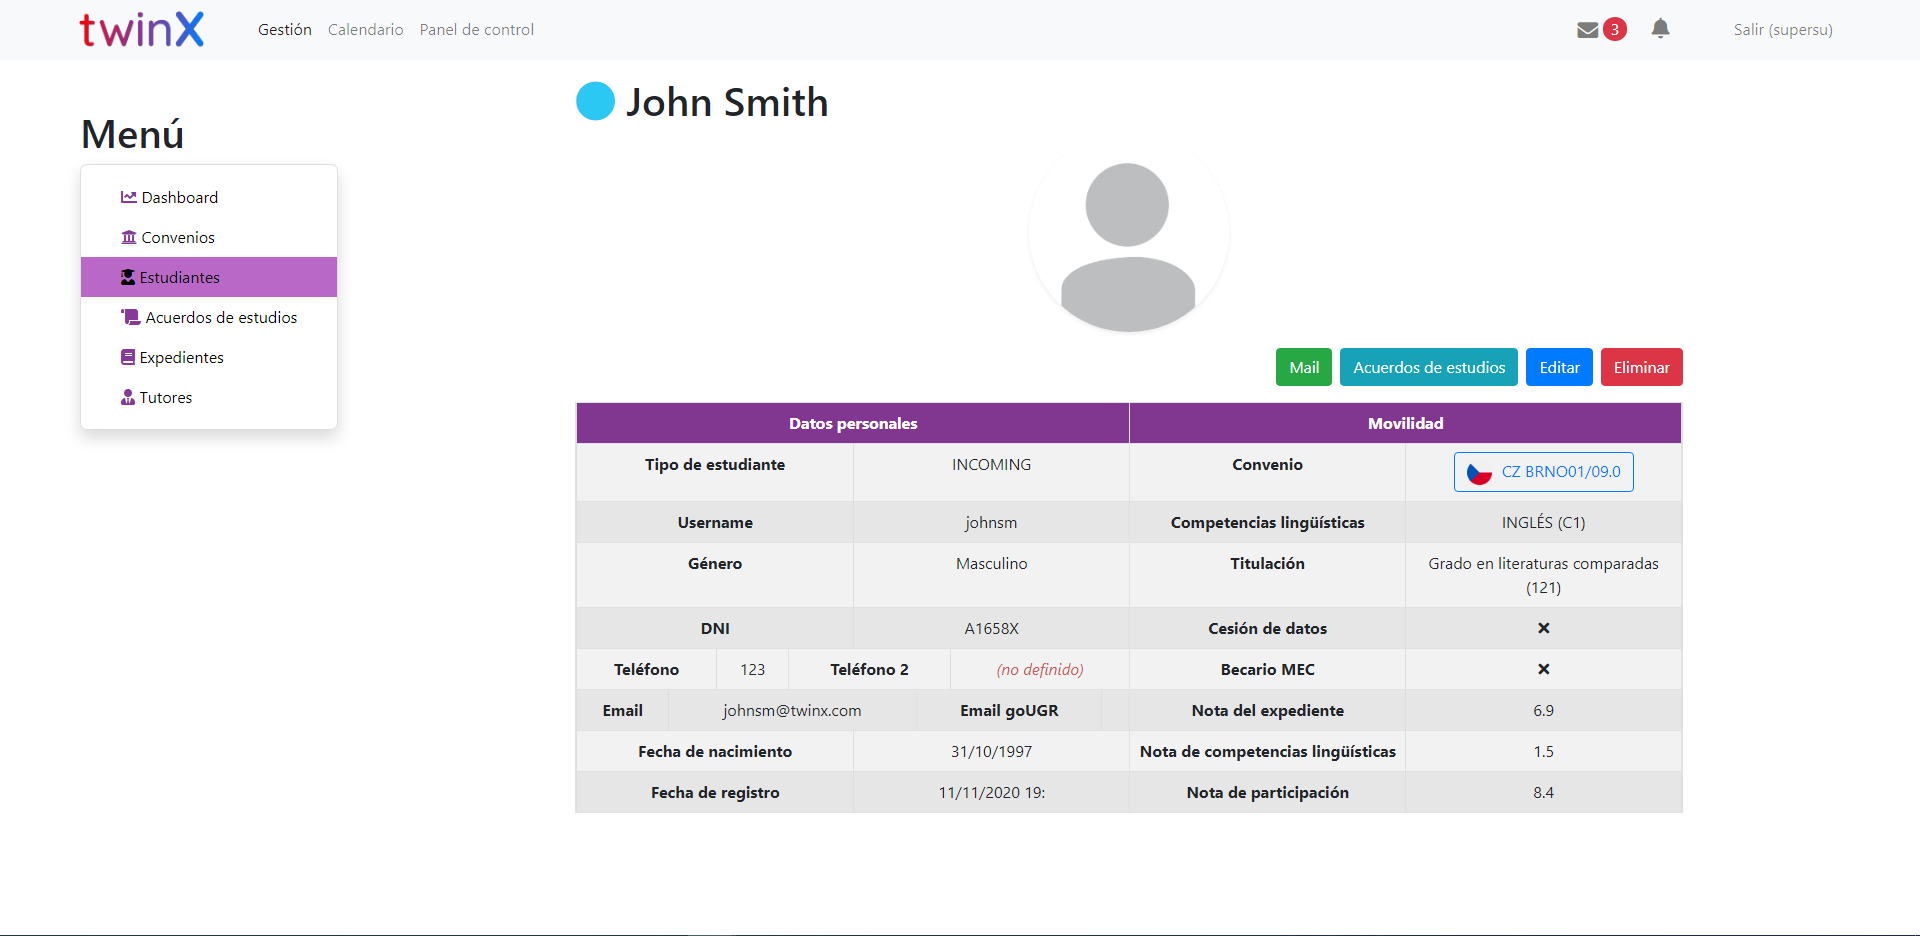
\includegraphics[width=\linewidth]{img/Capturas de twinX/vista_estudiante}
	\caption{Vista de estudiante en twinX}
	\label{fig:vistaestudiantetwinX}
\end{figure}

Llegados a este punto, señalamos la generación automática de la nota de competencia lingüística y de participación de un estudiante. En TWINS, ambas puntuaciones tenían que guardarse en dos atributos por separado, pero se ha creído conveniente desarrollar un algoritmo para el cálculo de las notas.
De acuerdo con las exigencias del convenio, si un estudiante tiene la misma competencia que se le requiere, no se le atribuye una nota extra. Sin embargo, a partir de B1 (que es lo mínimo que se puede requerir), se puede premiar con 1 punto adicional si el estudiante tiene un nivel B2, 1.5 puntos si es C1 o 2 puntos si su título es de C2, independientemente del nivel que se parta; esto es, si el estudiante tiene un C1 pero le requieren un B2 o B1, se le suman 1.5 puntos extra, y 2 puntos en caso de poseer un nivel C2 pero le requirieran C1 o inferior.

Entonces, en el modelo de \texttt{Estudiante}, el algoritmo es el siguiente:

\begin{minted}[frame=lines,breaklines]{php}
<?php
(...)
public function getNotaCompetenciaLing()
{
	$compConvenioRaw = $this->convenio->reqLingConvs;
	$compEstudianteRaw = $this->relClEsts;
	$compConvenio = [];
	$compEstudiante = [];
	$extra = 0;
	$valores = [
	'B1' => 0.5,
	'B2' => 1,
	'C1' => 1.5,
	'C2' => 2
	];
	
	foreach ($compConvenioRaw as $cC) {
		$compConvenio []= $cC->comp;
	}
	
	foreach ($compEstudianteRaw as $cE) {
		$compEstudiante []= $cE->cl;
	}
	
	foreach ($compEstudiante as $cE){
		if(in_array($cE, $compConvenio))
		unset($compConvenio[$cE->id]); // No tenemos en cuenta las competencias que requiere el convenio
	}
	
	foreach ($compEstudiante as $cE){
		foreach ($compConvenio as $cC){
			if($cE->lengua == $cC->lengua){
				if($valores[$cE->nivel] > $valores[$cC->nivel])
				$extra += $valores[$cE->nivel];
			}
		}
	}
	
	return $extra;
}

(...)
?>
\end{minted}

Entonces, el valor devuelto por el método es la nota de competencia lingüística que se muestra en la figura \ref{fig:vistaestudiantetwinX} y la nota de participación, la suma de ésta con la del expediente, ya es con esa nota con la que participa en el sorteo de las plazas de movilidad. Con este algoritmo, ahorramos un total de dos atributos en la tabla de estudiante, y teniendo en cuenta que la cantidad de registros a almacenar en el día a día es elevado, podemos considerar esta como una mejora significativa.

\subsection{Integración del menú de expedientes}

Sin pasar por el menú de acuerdos de estudios debida la carencia de novedades respecto a todo lo ya expuesto, que se repite a lo largo del desarrollo, entramos de lleno en los expedientes. Si bien ni el menú ni el formulario presentan características excesivamente novedosas, sí podemos encontrar un gran cambio en su vista (figura \ref{fig:vistaexpedientetwinX}).

\begin{figure}
	\centering
	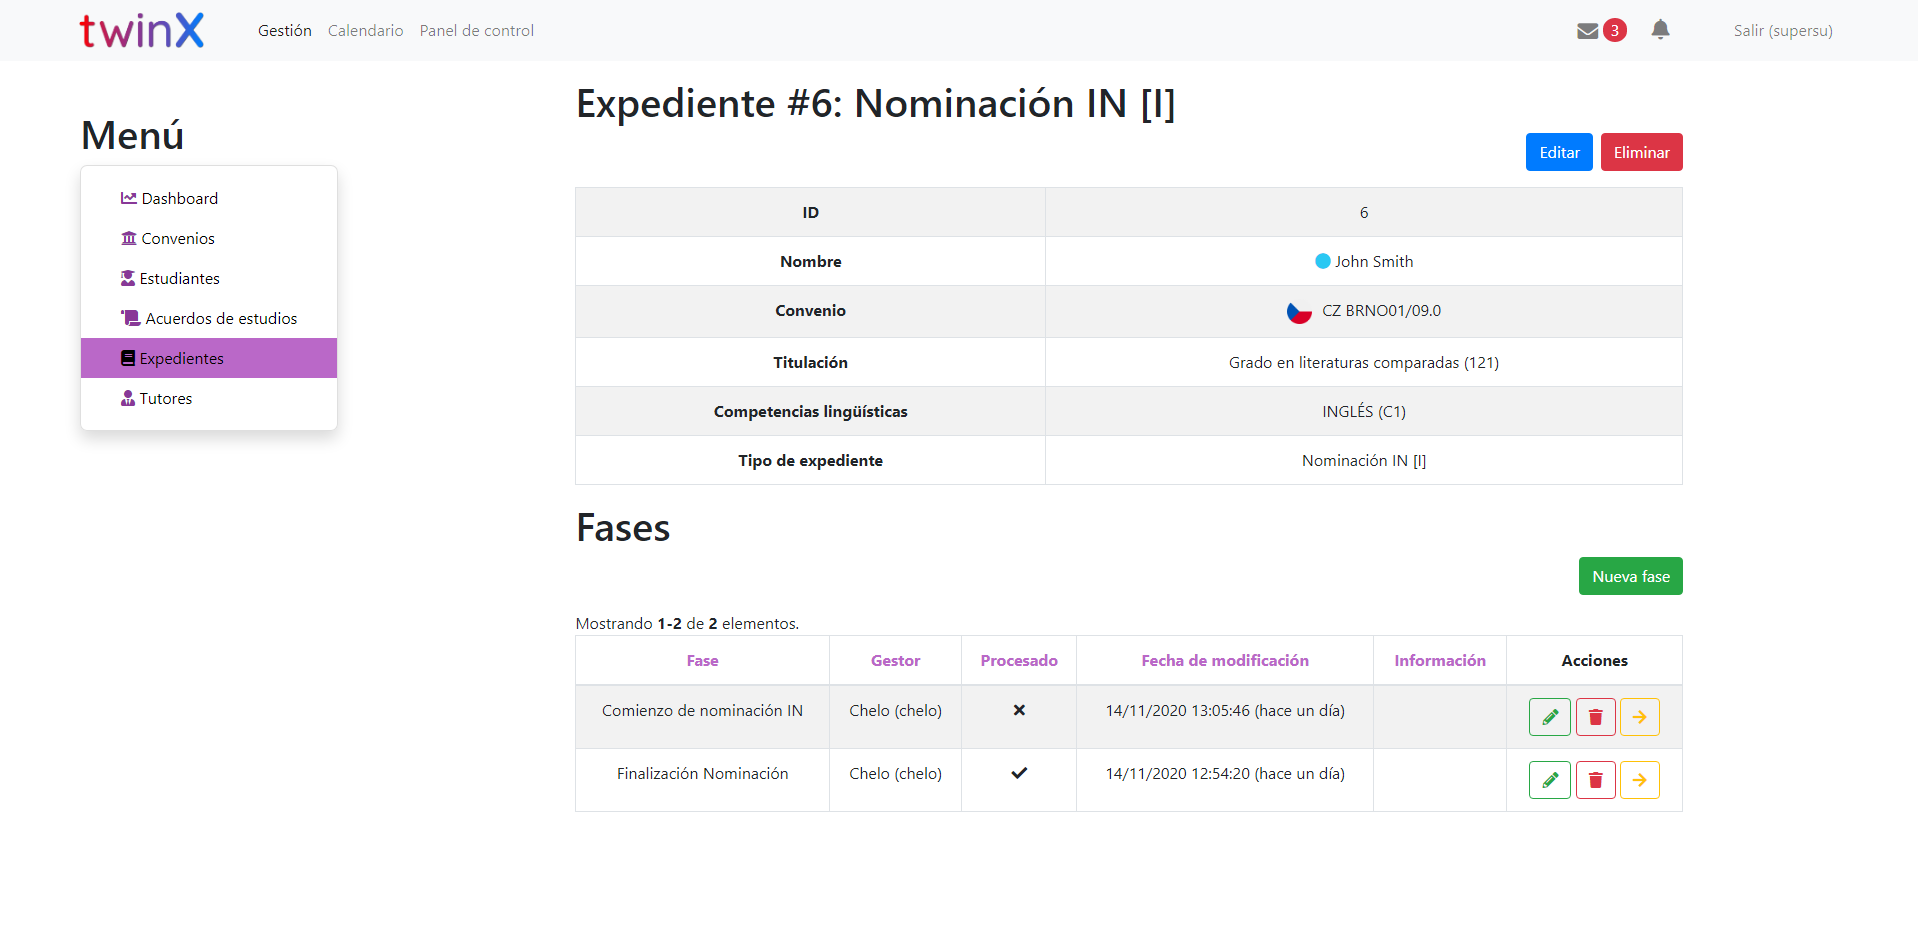
\includegraphics[width=\linewidth]{img/Capturas de twinX/vista_expediente}
	\caption{Vista de expedientes en twinX}
	\label{fig:vistaexpedientetwinX}
\end{figure}

Un expediente puede ser el de la nominación de un estudiante \textit{incoming}, y en todo momento necesitamos conocer en qué parte del proceso se encuentra su nominación. Recordemos que esto se posibilitaba con las \glspl{FaseExpedientetwinX}, y que cada una de ellas implicaba un envío de correos electrónicos en su \textbf{procesamiento}. Pues bien, al igual que en TWINS, lo más oportuno es ver el expediente del estudiante y su situación actual, con un historial de todo lo ya ocurrido en dicho registro. Esto lo hemos hecho posible embebiendo un menú en la interfaz de la vista del expediente; en este caso, aunque pueda pensarse que es el de la tabla \texttt{fase\_expediente}, en realidad se trata del de \texttt{rel\_fase\_exp} (relación de fase con expediente), donde se guarda información de la fase con respecto del expediente. De este último, aclaremos que en su tabla en la base de datos no se almacena otra información que la relación de un acuerdo y un tipo de expediente.

En este caso, aunque utilicemos la librería de JavaScript \textbf{AJAX} (integrada en Yii como \textbf{Pjax}), necesitamos crear vistas compuestas; esto es, vistas que mantengan la información del expediente en la parte de arriba mientras que en la parte de abajo se pueda estar renderizando el formulario de una fase o el menú que muestra todas las fases de un expediente. Estas dos últimas son las únicas posibilidades de variación de la interfaz que comentamos, pero volviendo al \textit{modus operandi} de Yii, recordemos que crear y actualizar son dos acciones distintas a ojos del controlador, aunque ambas usen el mismo formulario. Por tanto, necesitaremos los siguientes elementos:

\begin{itemize}
	\item \textbf{\texttt{\_view.php}}: donde almacenaremos la vista compartida y persistente de \texttt{Expediente}.
	\item \textbf{\texttt{view.php}}: la vista predeterminada con la información del expediente y sus fases.
	\item \textbf{\texttt{view-new-fase.php}}: carga la vista del expediente y el formulario de creación de una nueva fase.
	\item \textbf{\texttt{view-update-fase.php}}: carga la vista del expediente y el formulario de modificaicón de una fase ya existente.
\end{itemize}

Dentro de las tres últimas, llamamos a una instancia del controlador \\ \texttt{RelFaseExpController.php} desde el que se llama al menú, al creador y al actualizador respectivamente, en sus métodos \texttt{action} correspondientes:

\begin{minted}[frame=lines]{php}
	<?php include('_view.php') ?>
	
	<?= $relExpFase->actionCreate($model) ?>
	
	<?php $this->title = 'Expediente #' . $model->id; ?>
\end{minted}

Dado que en las tres vistas se precisa de una instancia del controlador, es en \texttt{\_view.php} donde se sitúa la creación de la misma:

\begin{minted}[frame=lines, breaklines]{php}
<?php
(...)

$relExpFase = new \backend\modules\gestion\controllers\RelExpFaseController('rel-exp-fase', Yii::$app->getModule('rel-exp-fase'));

(...)
?>
\end{minted}

Entonces, dado que es al controlador de \texttt{Expediente} al que se llama para cargar las distintas vistas compuestas (ya que nos situamos en \texttt{localhost/gestion/expediente}), es él mismo quien tiene que orquestar las llamadas a los métodos \texttt{action} para cargarlas, por lo que tenemos que crear acciones nuevas que llamen a los archivos de vista nuevos. A su vez y en aras de reutilizar código, éstos métodos harán una llamada a \texttt{actionView}, que es el mismo método que carga la vista del expediente, pero con nuevos parámetros, para que podamos enlazar el flujo de control con \texttt{RelExpFaseController.php}.

Una vez llegada la ejecución a uno de los archivos que permiten crear o modificar una fase para el expediente, se llama al método \texttt{actionCreate} o \texttt{actionUpdate} de \texttt{RelExpFase.php}, pero con una novedad: se pasa como argumento el \texttt{Expediente} actual, que por tanto el formulario ya tiene que llevar relleno en el campo destinado a ello. Lo mismo pasa con la actualización. En el caso de la vista de la lista de las fases de un expediente (archivo por defecto \texttt{view.php}), también se necesita el ID del expediente que se visualiza, para devolver tan solo aquellas fases pertenecientes al mismo. Esto se consigue modificando el método \texttt{actionIndex} de \texttt{RelExpFaseController.php} de la siguiente forma:

\begin{minted}[frame=lines, breaklines]{php}
<?php
(...)

public function actionIndex($idExpediente = false)
{
	$path = '';
	$query = RelExpFase::find();
	
	if($idExpediente) {
		$path = '@backend/modules/gestion/views/rel-exp-fase/';
		$query = $query->where(['id_exp' => $idExpediente]);
	}
	
	
	$dataProvider = new ActiveDataProvider([
	'query' => $query,
	]);
	
	return $this->render($path . 'index', [
	'dataProvider' => $dataProvider,
	'idExpediente' => $idExpediente,
	]);
}

(...)
?>
\end{minted}

Los métodos \texttt{actionCreate} y \texttt{actionUpdate} tienen una implementación similar. Nótese que no hemos impedido el funcionamiento corriente de los métodos, sino que los hemos complementado con atributos que poseen valores por defecto porque no siempre tienen que requerirse, en caso de necesitar hacer uso de la interfaz de forma independiente a la vista de expedientes como aquí se necesita. Toda esta estructura se tiene también para la visualización de los correos (\texttt{MailPredefinido}) que se envían en cada fase en el módulo del panel de control, cuya implementación es similar y por ello, no la hemos tratado.


\subsection{Integración del dashboard}

De nuevo, poco hay que decir sobre la implementación del menú de tutores, y por ello, pasamos a una de las grandes novedades que supone twinX sobre TWINS: la vista de dashboard (figura \ref{fig:dashboardtwinX}). Su objetivo no es otro que el presentar la información de mayor relevancia al usuario en cuanto abra la aplicación. Esta facilidad se ofrecía en TWINS en la forma de tres menús que bloqueaban toda la pantalla, ofreciendo información sobre el calendario, los avisos (mensajes en nuestro caso) y expedientes sin procesar, obligando al usuario a salir de las tres pantallas hasta llegar al menú principal. De esta manera, la aparición del dashboard no es bloqueante, y con tan solo una vista se resumen todos los asuntos que precisan de la atención del gestor al arrancar twinX.

\begin{figure}
	\centering
	\includegraphics[width=\linewidth]{img/Capturas de twinX/dashboard}
	\caption{Dashboard de twinX}
	\label{fig:dashboardtwinX}
\end{figure}

En este caso, no ha sido necesaria la creación de ningún menú CRUD ni ningún modelo nuevo. Simplemente hemos creado la vista \texttt{dashboard.php} en su directorio (\texttt{backend/modules/gestion/views/dashboard}) y en la carpeta de controladores, el \texttt{DashboardController.php}, poseedor de tan solo un método \texttt{actionIndex} que carga el archivo de la vista.

Dejando aparte las cuestiones de estilo, la información puede mostrarse a través de consultas a los demás modelos ya creados. Como mejora adicional, aunque aún no hayamos hablado de los mensajes y los recordatorios, vamos a presentar la última clase especial que tiene un gran potencial en Yii y de la cual hemos hecho uso en la implementación del dashboard. Son las clases \textbf{\texttt{Query}}. En ellas, cualquier método que se cree, puede ser ejecutado a modo de QBE a la hora de hacer una consulta a la base de datos, de modo que podamos ahorrar y reutilizar código. Por ejemplo, este es el método \texttt{notificaciones} de \texttt{RecordatorioQuery.php}:

\begin{minted}[frame=lines]{php}
<?php
(...)

public function notificaciones($db = null)
{
	return Recordatorio::find()
	->where(['id_usr_aviso' => Yii::$app->user->id])
	->andWhere(['<>', 'completado', '1'])
	->andWhere(['<', 'deadline', date('yy-m-d H:i')]);
}

(...)
?>
\end{minted}

Es sencillo, pero dado que en el dashboard necesitamos trabajar con las notificaciones pendientes en dos ocasiones (extraer el número de recordatorios pendientes y su vista de detalle en la sección de notificaciones), es muy práctico tenerlo para llamarlo de la siguiente manera:

\begin{minted}[frame=lines,breaklines]{php}
	<?php
	(...)
	
	$notificaciones = \common\models\Recordatorio::find()->notificaciones();
	
	(...)
	
	foreach ($notificaciones->with('emisor')->all() as $notificacion) {
		echo '<div class="card p-3 notificacion-dashboard mb-1">';
		$output = '<h5>Recordatorio</h5>';
		$output .= '<h6>' . $notificacion->titulo . '</h6> ';
		$output .= '<p>' . $notificacion->descripcion . '</p>';
		$output .= '<p class="text-muted d-flex flex-row-reverse">' . Yii::$app->formatter->asRelativeTime($notificacion->timestamp) . '</p>';
		echo \yii\helpers\Html::a($output, ['/calendario/recordatorio/view', 'id' => $notificacion->id]);
		echo '</div>';
	}
	
	(...)
	?>
\end{minted}

Es decir, en \texttt{\$notificaciones} almacenamos la \textit{query}, y la usamos llamando al método \texttt{count()} para obtener el número de registros o el array con todas ellas (\texttt{all()}) si necesitamos trabajar con cada una de ellas por separado.

En última instancia, es interesante también considerar la mejora que presenta la introducción de secuencias \texttt{width(<atributo>)}. Al especificar el \texttt{atributo} del modelo de la clase para la que se hace la consulta, se está evitando a toda costa lo que se conoce como el fenómeno de la «carga perezosa» o \textit{lazy loading}. Por ejemplo, para la carga de los expedientes sin procesar utilizamos varias sentencias \texttt{with} que nos permiten almacenar el contenido del atributo que se especifica, evitando posteriormente el tener que hacer consultas adicionales:

\begin{minted}[frame=lines,breaklines]{php}
	<?php
	foreach ($expedientes->with('exp')->with('exp.ae')->with('fase')->all() as $expediente) {
		echo '<div class="card p-3 notificacion-dashboard mb-1">';
		$output = '<h4>' . $expediente->exp->ae->estudiante->nombreEstudiante . '<h4>';
		$output .= '<h5>' . $expediente->exp->tipoExp->descripcion . '</h5> ';
		$output .= '<p>' . $expediente->fase->descripcion . '</p>';
		$output .= '<p class="text-muted d-flex flex-row-reverse">' . Yii::$app->formatter->asRelativeTime($expediente->timestamp) . '</p>';
		echo \yii\helpers\Html::a($output, ['/gestion/expediente/view', 'id' => $expediente->id_exp]);
		echo '</div>';
	}
	?>
\end{minted}

Es decir, como tenemos que recuperar atributos del acuerdo de estudios (\texttt{ae}) de \texttt{exp} y la \texttt{fase}, podemos ordenar que se almacenen los valores para no tener que recuperarlos de nuevo. Este comportamiento recibe el nombre de «carga entusiasta» o \textit{eager loading}. Más específicamente, sin ninguna orden \texttt{with} en toda la vista del dashboard, tendríamos un total de 45 \textit{queries}, mientras que con todas ellas, rebajamos el número hasta 38.

\subsection{Integración de la mensajería}

Por último en este módulo, hemos implementado la mensajería de twinX (figura \ref{fig:bandejaentradatwinX}). En lugar de tener un \texttt{actionIndex} en \texttt{MensajeController.php} general para la lista de mensajes, se ha sustituido por un \texttt{actionRoute}, que diverge la vista del menú en bandeja de entrada o elementos: enviados y carga los mensajes que mostrar en función de si se es emisor o receptor de los mismos:

\begin{minted}[frame=lines]{php}
<?php
(...)
public function actionRoute($bandeja)
{
	$searchModel = new MensajeSearch();
	$query = $searchModel->searchQuery(Yii::$app->request->queryParams);
	
	if($bandeja == 'INBOX')
		$query->andWhere(['id_receptor' => Yii::$app->user->id]);
	else
		$query->andWhere(['id_emisor' => Yii::$app->user->id]);
	
	$dataProvider = $searchModel->search($query);
	
	return $this->render('index', [
		'searchModel' => $searchModel,
		'dataProvider' => $dataProvider,
		'bandeja' => $bandeja
	]);
}
(...)
?>
\end{minted}


\begin{figure}
	\centering
	\includegraphics[width=\linewidth]{img/Capturas de twinX/bandeja_entrada}
	\caption{Bandeja de entrada en twinX}
	\label{fig:bandejaentradatwinX}
\end{figure}

De la vista de menú, se ha creído conveniente crear un pequeño atajo para marcar un mensaje como leído o no leído. También se ha tratado de simplificar la vista (figura \ref{fig:vistamensajetwinX}) condensando los atributos de valor de un mensaje en su cabecera y su asunto como título del contenido. Destaca también la ausencia de opciones como la edición y eliminación de un mensaje ya enviado, para mantener el significado de la entidad \texttt{Mensaje} y no tratarla como una tupla más de una tabla en base de datos.

\begin{figure}
	\centering
	\includegraphics[width=\linewidth]{img/Capturas de twinX/vista_mensaje}
	\caption{Vista de mensaje en twinX}
	\label{fig:vistamensajetwinX}
\end{figure}


\section{Desarrollo del módulo de calendario}

La parte del calendario en TWINS podía resultar un poco confusa al tratar de entender cómo funciona: un calendario con eventos comunes a todo el mundo. Estos eventos con un máximo de dos personas a las que poder avisar, tenían la capacidad de encontrar asociadas numerosas tareas que dividían el evento en distintas etapas. Las tareas, a su vez, contaban con otro máximo de dos personas a las que poder asignar esa tarea y con una fecha límite concreta. Tenían características incluso como la atribución de un porcentaje de progresión en la completitud de la tarea o también el evento (figura \ref{fig:nuevatarea}).

En el boceto de la figura \ref{fig:nuevo_eventoWF} representamos una aproximación a lo que podría ser el calendario en twinX, pero aunque quizás no tan complicado de implementar, su desarrollo necesita bastante tiempo, ya que en twinX, de acuerdo con el modelo de la base de datos (figura \ref{fig:modeloBD}), se tenía una relación muchos a muchos para poder avisar a cuantos gestores se quisiera para un evento o una tarea creados. Esto complica la implementación, haciéndola menos inmediata e inteligible, pues pensemos que tendríamos que desempeñar de nuevo las mismas acciones que para generar vistas compuestas; en este caso, varias tablas CRUD embebidas, unas dentro de otras.

Ya hemos demostrado que es posible hacer este tipo de direccionamiento de los flujos de información para obtener los resultados que se quieren, pero por motivos de tiempo, se ha decidido cambiar la implementación de esta parte por otra, dentro del módulo del calendario, ya que no afecta a la consecución de los objetivos generales del proyecto. Más concretamente, al comienzo del segundo sprint \ref{subsubsec:segundosprint} se tomó la decisión de dejar fuera de la programación la \hyperref[tab:HU3.1]{HU3.1} y la \hyperref[tab:HU3.2]{HU3.2}. En consecuencia, se pudo llevar a cabo el desarrollo de la \hyperref[tab:HU3.3]{HU3.3} y la \hyperref[tab:HU4]{HU4} con mayor margen temporal y con la posibilidad de establecer un mayor enfoque en los resultados y la calidad de los mismos con respecto, como siempre, a los objetivos generales del proyecto.

Sobre la codificación de esta parte, las tareas a realizar eran similares: creación de un módulo, generación del modelo de \texttt{Recordatorio} y del menú CRUD para el mismo. Hemos, sin embargo, filtrado la aparición de recordatorios en el menú principal (figura \ref{fig:recordatoriostwinX}) a tan solo los que crea el usuario. Cabe destacar que un gestor puede dirigir recordatorios a otro compañero, por lo que le aparecerán en su menú. Sin embargo, si otro usuario crea un recordatorio para nosotros, no lo veremos ahí, sino en la sección de notificaciones, que tiene también un testigo rojo a modo de contador en la cabecera de la web para que nos demos cuenta siempre que tengamos alguno pendiente. También aparecen en el dashboard, por lo que al abrir la aplicación no solo veríamos que tendríamos un recordatorio pendiente, sino que también podríamos apreciar de qué se trata. Si hacemos clic en él, nos redirigirá a la vista de detalle, muy similar a la de los mensajes. Una vez se marcan como completados, desaparecerán de notificaciones.

\begin{figure}
	\centering
	\includegraphics[width=\linewidth]{img/Capturas de twinX/recordatorios}
	\caption{Menú de recordatorios en twinX}
	\label{fig:recordatoriostwinX}
\end{figure}

Para las notificaciones no nos ha hecho falta crear otro modelo, tan solo una vista y un controlador sencillos, al igual que para el dashboard, ya que las consultas que se hacen a la base de datos se realizan sobre instancias de modelos ya creados. Retomemos la utilidad de haber construido el método en \texttt{RecordatorioQuery.php} para recuperar todos los recordatorios pendientes para explicar el funcionamiento de \texttt{actionIndex} en \texttt{NotificacionesController.php}; ahorramos aún más código:

\begin{minted}[frame=lines]{php}
<?php
(...)

class NotificacionesController extends \yii\web\Controller
{
	public function actionIndex()
	{
		$dataProvider = new ActiveDataProvider([
		'query' => Recordatorio::find()->notificaciones()
		]);
		
		return $this->render('index', [
		'recordatorios' => $dataProvider
		]);
	}
}

?>

\end{minted}

A modo de resumen, podemos elaborar el diagrama de paquetes de la figura \ref{fig:diagramapaquetes} para ver la disposición de los archivos del proyecto en sus paquetes y directorios y la interacción entre los mismos. Se ha omitido el contenido de cada uno de los subdirectorios de \texttt{views} por motivos de extensión del diagrama, al igual que de los directorios \texttt{query} y \texttt{search}, que no aportan nombre de clases nuevas.

\begin{figure}
	\centering
	\includegraphics[width=\linewidth]{img/diagrama_paquetes}
	\caption{Diagrama de paquetes de twinX}
	\label{fig:diagramapaquetes}
\end{figure}

% 7. Pruebas

\chapter{Pruebas}
\label{pruebas}

Una vez creada la primera versión de twinX, el siguiente paso es evaluar el trabajo llevado a cabo. Para ello, nos guiaremos por una serie de pruebas de las que poder obtener retroalimentación sobre si el software cumple las expectativas o si por lo contrario necesita mejoras, en contraposición de lo planeado en el desarrollo del proyecto.

\section{Pruebas de usabilidad}

En primer lugar, vamos a desarrollar cómo fueron las pruebas de usabilidad de twinX. La utilidad de estas pruebas está en conocer cuán buena es la disposición de los elementos del sitio y si su funcionamiento es adecuado, mediante la evaluación de la interacción de los usuarios con twinX.

Para llevarlas a cabo, se solicitó a dos usuarios que trabajan en la ORI-FyL que usaran la aplicación. Más concretamente, se les instó a que realizaran una serie de tareas en la web tras tener acceso a ella, sin darles ningún indicio de dónde tenían que acudir para llevar a cabo la tarea encomendada. De este modo, comprobamos si es o no sencillo utilizar twinX y qué mejoras se pueden hacer basadas en la interacción del usuario con la plataforma. Por ejemplo, si a la hora de realizar una acción que se solicite, todos los usuarios llevados a examen realizan la misma acción de forma errónea, entonces podemos afirmar que la aproximación propuesta tras el desarrollo no es válida, pues no funciona como se espera, y hace a los usuarios perder tiempo y la concentración con respecto a la consecución de sus objetivos.

Las sesiones de prueba se llevaron a cabo a través de Google Meet \cite{googlemeet} y se pidió permiso a los asistentes para grabar la sesión, de modo que pudiera ser examinada \textit{a posteriori}. A los usuarios se les solicitó que no entraran juntos a la sala de reunión para no conocer de partida el funcionamiento de la web antes de enfrentarse a las pruebas. Antes de ponernos manos a la obra, se les dio una pequeña introducción con unas pautas sencillas \cite{krug} y que hacían la sesión más fructífera y natural tanto para el evaluador como para los evaluados. Entre ellas, destacan las siguientes:

\begin{itemize}
	\item \textbf{Pensar en voz alta:} cualquier apreciación es buena. Pensamientos como «imagino que si pulso este botón iré a esta otra parte...» o «vaya, creía que iba a encontrar otra cosa» ayudan a la mejora y a reconsiderar las decisiones tomadas.
	\item \textbf{El usuario sometido a pruebas nunca se equivoca:} en todo caso, el fallo lo comete el desarrollador por haber pensado que algo podía ser buena idea pero finalmente termina confundiendo al usuario.
	\item \textbf{No complicarse la vida, actuar como se crea:} de lo contrario, el portal sería difícil de comprender, lo que no es beneficioso en absoluto.	
\end{itemize}

En twinX ya había cierta información introducida, como algunos estudiantes, países, universidades, tipos de expedientes y sus fases, y convenios, sobre todo, ya que albergan mucha información y tampoco sería apropiado excederse en tiempo haciendo pruebas con el usuario.

Las tareas que se solicitaron llevar a cabo a ambos usuarios fueron las siguientes:

\begin{enumerate}
	\item \textbf{Crear un acuerdo de estudios a uno de los estudiantes almacenados:} para ello hay que ir al apartado de acuerdos de estudios, situado en el menú de la izquierda en la sección de «gestión», que es la que se abre por defecto al entrar a twinX. Una vez allí, hay que pulsar el botón verde en la esquina superior derecha de la tabla y rellenar el formulario que se muestra a continuación.
	\item \textbf{Comprobar que el convenio tiene asociado el nuevo acuerdo de estudios:} de nuevo en el menú de la izquierda, hay que ir al apartado de convenios y buscar el convenio para el que se ha creado el acuerdo de estudios. Dentro de la vista, hay que desplegar la parte llamada «acuerdos de estudios» y ver que, efectivamente, figura el acuerdo de estudios que se acaba de crear asociado al estudiante correspondiente.
	\item \textbf{Crear un expediente para el acuerdo creado:} en el apartado de expedientes, hay que seleccionar la opción de «nuevo expediente». En el formulario, rellenar con el acuerdo de estudios que se ha creado en la primera tarea y seleccionar el tipo de expediente.
	\item \textbf{Introducir una primera fase para el expediente que se acaba de crear:} una vez creado, twinX redirige al usuario a la vista de expediente con sus fases en una tabla que se encontrará vacía de forma preliminar. A continuación, el usuario tiene que pulsar el botón de «nueva fase» y guardar los cambios. Una vez se muestra la lista con las dos fases asociadas al expediente, habría que pulsar en el botón con la flecha para procesar la fase. Se abrirá un cuadro de diálogo que hay que aceptar para completar el proceso.
	\item \textbf{Crear una nueva fase final para el tipo de expediente con el que se está trabajando:} en esta ocasión, la tarea requiere salir de la sección de «gestión» y dirigirse al panel de control. Allí, seleccionar el menú «expedientes», después de lo cual se desplegará un menú con otras dos opciones. Hay que escoger la de «fases de expedientes» y crear ahí una nueva fase para el tipo de expediente que se ha abierto al estudiante en la tercera tarea, marcando la opción de «fase final».
	\item \textbf{Cambiar el expediente a la fase recién creada:} volver a «gestión», en el menú del expediente con el que estamos trabajando. De nuevo, volver a asociar una nueva fase (la creada).
	\item \textbf{Consultar los acuerdos de estudios que tiene un tutor:} tan solo habría que ir al menú de tutores y buscar el único tutor que hay en la plataforma creado y al que se le puede asociar un acuerdo de estudios. Allí, hay que seleccionar la única acción disponible, que es un botón con un pergamino (el mismo icono que tienen los acuerdos de estudios) para acceder a una vista donde se muestran todos los acuerdos que tutoriza dicha persona. 
\end{enumerate}
%«Modificación del acuerdo OUT» (usuario A) y «Nominación IN» (usuario B)


\subsection{Sesión de pruebas del usuario A}

Para el usuario A, el desarrollo de las tareas (en el mismo orden que las hemos presentado) ha sido el siguiente:

\begin{enumerate}
	\item Primeramente se dirigió al menú de estudiantes. Al ver en la tabla que para cada estudiante tenía dos posibles acciones, reconoció que una era para ver los detalles del estudiante (botón del ojo) y el otro (universidad, para acceder a su convenio), no lo reconocía. Por tanto, puso el ratón encima y tal y como estaba previsto, apareció la ayuda textual que señalaba que era un botón para ir al convenio del estudiante. Entonces, cambió de estrategia y fue al menú de acuerdos de estudios, donde finalmente encontró la forma de desarrollar la tarea solicitada.
	\item A pesar de haber un botón en el acuerdo de estudios como acceso directo al convenio, que es donde se tenía que dirigir, fue al listado de todos los convenios y buscó el convenio para el cual se había creado el acuerdo. Al entrar en la vista del convenio, no reconoció dónde estaban sus acuerdos asociados; es decir, no supo interpretar que cada una de las categorías era desplegable y que al pulsarlas se vería nueva información tal y como se pensaba en el desarrollo que sugeriría la flecha hacia abajo de desplegable. Entonces, volvió al menú de acuerdos, donde anunciaba que efectivamente el acuerdo se había creado porque aparecía ahí. Sin embargo, se volvió a pedir al usuario que lo visualizara desde la vista del convenio. Volvió a la misma vista de antes y se paró a leer los enunciados de los desplegables. Daba la sensación de que en su primera visita, en el primerísimo vistazo, pensaba que las distintas secciones era más información del convenio. Al leer el de «acuerdos de estudios», efectivamente pulsó y comprobó lo que se le había solicitado.
	\item Para la creación del expediente, el usuario fue al menú del acuerdo creado, pensando que al entrar a verlo habría un botón para crear un expediente. Pero no encontró nada. Al percatarse de ello, fue al menú de expedientes, donde sí pudo ver de nuevo el botón verde que le permitía crear una nueva entrada.
	\item Al situarse justo debajo del acuerdo el botón que le permitía crear una nueva fase, el usuario A lo encontró rápidamente y pudo crear la fase en cuestión de segundos. Para procesar la fase, volvió a analizar los botones representando las tres acciones acompañadas de los iconos del lápiz, la papelera y la flecha. Supuso que éste último era para lo que buscaba y la ayuda de texto al posicionar el cursor encima se lo confirmó, pero también optó por hacerlo editando el registro y marcando la casilla «procesada» en el formulario de edición.
	\item Para explicar esta tarea, se pidió que volviera a crear una fase al expediente, y comprobó que efectivamente había solo una fase. Entonces, una vez comprendió el problema, fue muy directo al panel de control. Allí se desorientó un poco y se puso a observar todos los detalles. Entonces, tras recordarle la tarea, y tras haber leído todas las opciones del menú en la primera pasada, desplegó el menú correspondiente y accedió a la parte de «fases de expedientes». Una vez allí, creó la fase sin problema.
	\item Casi sin pedírselo y prácticamente curioseando, volvió a «gestión», a expedientes, creó la fase, la dejó sin procesar. Libremente se dirigió al dashboard, comprobó que había una fase sin procesar. Volvió atrás, procesó la fase y comprobó una vez más que en el dashboard no quedaba ninguna fase pendiente.
	\item Accedió al menú de tutores sin problema y pulsó sobre la única acción que había en el registro del tutor, completando la tarea y terminando, así, las pruebas.
\end{enumerate}

Este usuario se tomó muy en serio, afortunadamente, el «pensar en voz alta», lo que fue bastante positivo para poder comprender cómo pensaba. Hizo muchos comentarios como «me iría aquí...» o «supongo que si hago clic aquí, aparecerá esto otro...». También le llamó la atención el dashboard, y lo consultó por cuenta propia para ver que efectivamente, tras procesar un expediente, el registro desaparecía del resumen de «expedientes sin procesar», lo cual es bastante positivo. Además destaca la gran confianza que adquirió en la penúltima tarea, pues parecía haber estado trabajando con la aplicación anteriormente y denotaba haber comprendido muy bien la disposición de los elementos en la misma.

\subsection{Sesión de pruebas del usuario B}


Siguiendo el mismo orden, el otro usuario realizó también sus tareas como describimos:

\begin{enumerate}
	\item De nuevo, este usuario fue al menú de estudiantes. Se situó en el estudiante que se le indicó y cargó su vista. Una vez allí, trató de editar sus datos. Estuvo mirando otras características y probando otras funciones, como la de enviar mail al estudiante. Una vez volvió, sí fue directamente al menú de acuerdo de estudios y creó el convenio correctamente.
	\item Al haber estado en el paso anterior ojeando cómo son las vistas de los convenios, no le fue nada difícil encontrar el camino hacia el objetivo. Adicionalmente, reconoció el significado de la columna «nominados totales» del menú de convenios, algo muy positivo, ya que supone un gran cambio en cuanto a la visualización del mismo dato existente en TWINS (los primeros cuadros de colores en la figura \ref{fig:vistaConvenios}).
	\item Esta tarea fue también muy rápida, pues hizo click directamente en el menú de expedientes y en el botón verde de «nuevo expediente».
	\item De nuevo, al aparecer el botón de «nueva fase» en la vista tras crear el expediente, supo seguidamente crearla. Para procesarla, estuvo dudando sobre el botón de edición, el del lápiz --sobre el que posó el ratón--,  y el de «procesar fase». Finalmente, pulsó este último y aceptó el diálogo que concluía con esta tarea.
	\item Para esta tarea, tras la explicación, estuvo dudando bastante sobre cómo hacerlo: intentó escribir en el campo de búsqueda de la fase, fue atrás, hacia el menú de la vista de las fases del expediente, trató de editar el expediente del estudiante, pero ahí no estaba la opción. Finalmente, se le dieron indicaciones para que prestara atención a la cabecera de la web, la cual no había tomado como tal y desconocía que se albergaban más opciones ahí. Tras volver a curiosear entre las nuevas posibilidades que había descubierto, se dirigió al panel de control. Una vez allí, al menú de fases de expedientes, pero comenzó a introducir la nueva información en los campos destinados a la búsqueda. Sin la ayuda de nadie, se dio cuenta, y volvió a ejecutar las acciones desde el principio (en lugar de borrar su búsqueda o darle al botón de «nuevo expediente»). De nuevo en el menú correspondiente, ya sí supo crear lo que se le requirió.
	\item Al igual que el usuario A, recordó los pasos que había que hacer para volver a cambiar el expediente de fase. No obstante, tuvo la iniciativa de intentar llegar al mismo sitio siguiendo otro camino, pero finalmente tuvo que reproducir los pasos anteriores. Hizo clic en procesar la fase que ya habíamos procesado anteriormente, pero se dio cuenta a tiempo de que justo es lo que había hecho antes y no lo que se le solicitaba ahora, y canceló el diálogo a tiempo. Después, cambió el expediente a la fase recién creada.
	\item Esta tarea también fue muy sencilla para el usuario B y pudo completarla en cuestión de segundos.
	
\end{enumerate}

Del usuario B destacamos la gran curiosidad que tenía por descubrir cosas por su cuenta y ver los cambios que presentaba twinX. Algo de lo más positivo al hacer pruebas, fue su actitud «caótica» a la hora de ejecutar las acciones sin pensar, pues se dejaba llevar por su instinto y permitía ver las cosas que realmente estaban bien y las que no tanto. También comparaba algunas pequeñas carencias que no tenía TWINS respecto de twinX provenientes del uso diario de la aplicación, como un aumento de los accesos directos para ir fácilmente de una entidad a otra (por ejemplo, de la vista de estudiante a sus expedientes).

\subsection{Encuestas SUS}

Al final de la sesión, se ofreció a los individuos una encuesta SUS para que la cumplimentaran y así poder obtener más información de su experiencia. La rellenaron mediante los Formularios de Google \cite{googleforms}, y sus respuestas fueron los de las tablas \ref{tab:sus1} y \ref{tab:sus2}

\subsubsection*{Resultado 1}

\begin{table}[H]
	\begin{center}
		\begin{adjustbox}{width=\textwidth}
			\begin{tabular}{ | c | c | c | c | c | c | } 
				\hline
				\textbf{Pregunta} & 1 & 2 & 3 & 4 & 5 \\
				\hline
				Creo que utilizaría twinX con frecuencia &  &  &  &  & X \\
				\hline
				Encuentro twinX innecesariamente complejo &  X &  &  &  &  \\
				\hline
				Pienso que twinX es sencillo de usar &  &  &  &  & X \\
				\hline
				Considero que necesitaría la ayuda de una persona especializada para usar el sistema & X &  &  &  &  \\
				\hline
				Encuentro las funcionalidades de twinX bien integradas &  &  &  & X &  \\
				\hline
				Veo que hay mucha inconsistencia en el sistema & X &  &  &  &  \\
				\hline
				Imagino que la gente aprenderá rápido a usar twinX &  &  &  &  & X \\
				\hline
				Creo que twinX es demasiado engorroso para mí & X &  &  &  &  \\
				\hline
				Me siento muy seguro/a de mí mismo/a utilizando twinX &  &  &  &  & X \\
				\hline
				Necesitaría aprender bastantes cosas antes de comenzar a usar twinX & X &  &  &  &  \\
				\hline
			\end{tabular}
		\end{adjustbox}
		\caption{Resultado de la encuesta SUS 1}
		\label{tab:sus1}
	\end{center}
\end{table}

\subsubsection*{Resultado 2}

\begin{table}[H]
	\begin{center}
		\begin{adjustbox}{width=\textwidth}
			\begin{tabular}{ | c | c | c | c | c | c | } 
				\hline
				\textbf{Pregunta} & 1 & 2 & 3 & 4 & 5 \\
				\hline
				Creo que utilizaría twinX con frecuencia &  &  &  &  & X \\
				\hline
				Encuentro twinX innecesariamente complejo &  X &  &  &  &  \\
				\hline
				Pienso que twinX es sencillo de usar &  &  &  &  & X \\
				\hline
				Considero que necesitaría la ayuda de una persona especializada para usar el sistema &  &  &  &  & X \\
				\hline
				Encuentro las funcionalidades de twinX bien integradas &  &  &  &  & X \\
				\hline
				Veo que hay mucha inconsistencia en el sistema & X &  &  &  &  \\
				\hline
				Imagino que la gente aprenderá rápido a usar twinX &  &  &  &  & X \\
				\hline
				Creo que twinX es demasiado engorroso para mí & X &  &  &  &  \\
				\hline
				Me siento muy seguro/a de mí mismo/a utilizando twinX &  &  &  & X &  \\
				\hline
				Necesitaría aprender bastantes cosas antes de comenzar a usar twinX &  & X &  &  &  \\
				\hline
			\end{tabular}
		\end{adjustbox}
		\caption{Resultado de la encuesta SUS 2}
		\label{tab:sus2}
	\end{center}
\end{table}

\subsection{Conclusiones de las pruebas de usabilidad}

La respuesta de los usuarios ante las tareas solicitadas para ser llevadas a cabo ha sido muy positiva, si bien hay que tener en cuenta las confusiones que han tenido momentáneamente, que en ocasiones acompañaban a la personalidad del usuario y su forma de interaccionar con una interfaz completamente nueva.

Gracias a las pruebas realizadas, se puede comenzar desde ya a mejorar twinX incluso en su primera versión, sin planificar nuevas historias de usuario. Estas aportaciones son posibles debido a que los usuarios con los que se han hecho las pruebas trabajan en la oficina, lo que nos lleva a pensar que, como es lógico, el probar twinX en su misma atmósfera de trabajo tendría como resultado su exponencial potenciación a base de la diaria observación de la interacción con el actual TWINS, teniendo aún más información de aspectos que mejorar, a pesar del cambio que supone la nueva plataforma.

Sobre las encuestas, hay que clarificar que se han dispuesto en un orden aleatorio y que no se conoce cuál pertenece al usuario A y cuál al B. Para analizar mejor su resultado, vamos a dividir las preguntas en dos grupos: positivas y negativas (tabla \ref{tab:resultadossus}). Las primeras serán aquellas para las que cuantos más puntos se obtenga, más positiva será la valoración y viceversa. 

\begin{table}[H]
	\begin{center}
		\begin{adjustbox}{width=\textwidth}
			\begin{tabular}{ | c | c | c | } 
				\hline
				\textbf{Categoría} & \textbf{Preguntas} & \textbf{Puntuación} \\
				\hline
				\multirow{5}{*}{Positivas} &
				Creo que utilizaría twinX con frecuencia  & \multirow{5}{*}{48/50} \\
				\cline{2-2}
				& Encuentro las funcionalidades de twinX bien integradas & \\
				\cline{2-2}
				& Pienso que twinX es sencillo de usar &  \\
				\cline{2-2}
				& Imagino que la gente aprenderá rápido a usar twinX & \\
				\cline{2-2}
				& Me siento muy seguro/a de mí mismo/a utilizando twinX &  \\
				\hline
				\multirow{5}{*}{Negativas}& Encuentro twinX innecesariamente complejo & \multirow{5}{*}{15/50} \\
				\cline{2-2}
				& Considero que necesitaría la ayuda de una persona especializada para usar el sistema & \\
				\cline{2-2}
				& Veo que hay mucha inconsistencia en el sistema & \\
				\cline{2-2}
				& Creo que twinX es demasiado engorroso para mí & \\
				\cline{2-2}
				& Necesitaría aprender bastantes cosas antes de comenzar a usar twinX &\\
				\hline
			\end{tabular}
		\end{adjustbox}
		\caption{Resultado de las encuestas SUS}
		\label{tab:resultadossus}
	\end{center}
\end{table}

Es observable que en los aspectos positivos se roza el máximo de 50 puntos, mientras que por lo bajo, también se acerca a 10, siendo ésta la puntuación mínima, por lo que podemos apreciar que los resultados han sido buenos.

Si quisiéramos obtener un resultado sobre 100 acerca de cuán bien les ha parecido twinX a los usuarios, podríamos seguir las directrices que se indican en \cite{susscore}. Hemos de restar un punto a las preguntas impares y sustraer a 5 el valor de las pares. El resultado de sumar los nuevos valores y multiplicar por 2.5 daría, en cada encuesta, el resultado sobre 100. En el primer caso, habríamos obtenido una puntuación de 97.5 puntos y, en el segundo de 85 puntos. Sobre esta última, en un intento de comprender la respuesta a la pregunta «considero que necesitaría la ayuda de una persona especializada para usar el sistema», contestada con 5 (totalmente de acuerdo), podría ser por la necesidad de comprender el funcionamiento de la oficina, ya que basándonos en el resto de sus respuestas, parece haber tenido una buena experiencia tras las pruebas; es más, la puntuación que obtenemos es de 85/100, cuando 68 sería la media según la fuente que citamos.

En resumen, parece que el trabajo hecho con twinX no se distancia mucho de la línea en que desarrollan su trabajo en la ORI-FyL, por lo que podemos entender que se están consiguiendo los objetivos propuestos para el proyecto.

\section{Pruebas de accesibilidad}

Tal y como comentamos en la sección \ref{subsec:accesibilidad}, no todo el mundo tiene las mismas necesidades, y es hora de conocer si nuestro sitio web reúne una serie de condiciones mínimas para la visualización por personas con alguna discapacidad.

Por lo general, los resultados arrojados no son malos. La puntuación más baja que se ha obtenido ha sido la de 79/100 (figura \ref{fig:testaccesibilidad}), específicamente en las vistas de menú, donde los botones de la tabla (columna «acciones») tienen un icono visual y no un texto. Este problema se podría resolver fácilmente ofreciendo un texto alternativo para cada botón, de modo que un asistente de voz pueda leer la web, a pesar de tener elementos gráficos.


\begin{figure}
	\centering
	\includegraphics[width=\linewidth]{img/test_accesibilidad}
	\caption[Resultados de las pruebas de accesibilidad]{Resultados de las pruebas de accesibilidad en la mayoría de las vistas de menú}
	\label{fig:testaccesibilidad}
\end{figure}

Además, aunque de menor importancia, se han detectado anomalías en cuanto al poco contraste entre el fondo y el contenido, de manera que las personas con una visión reducida podrían tener problemas al visualizar la web. Podríamos, en este caso, ofrecer una visualización alternativa en cuanto al esquema de colores respecta, ya que no sería muy complicado aplicar unas cuantas reglas adicionales y que se ejecutaran de forma opcional para las personas con este tipo de necesidades.

Sobre la lacra de etiquetas en los campos de un formulario que detecta Lighthouse \cite{lighthouse}, es en este caso en el lado de la clase que renderiza los campos de búsqueda de la tabla del menú, que probablemente puedan configurarse de alguna manera, solo que al ser generados de forma automática, no se les ha prestado gran atención a los mismos.

\section{Credenciales para la prueba en primera personad de twinX}

Para poder experimentar el funcionamiento de twinX (accesible en \cite{twinx}) y ejecutar una serie de pruebas, se pone a disposición del lector las siguientes credenciales:

\begin{itemize}
	\item Entorno de \gls{gestortwinX}:
	\begin{itemize}
		\item \textbf{Nombre de usuario:} gestor
		\item \textbf{Contrseña:} gestor	
	\end{itemize}
	\item Entorno de \gls{administradortwinX}:
	\begin{itemize}
		\item \textbf{Nombre de usuario:} administrador
		\item \textbf{\textsc{Contraseña}:} administrador	
	\end{itemize}
\end{itemize}




% 8. Distribución de producto

\chapter{Distribución del producto}

Para poder usar twinX, dado que está pensado para ser accedido desde la web, tenemos que tenerlo primeramente alojado en un servidor, de modo que pueda ser accesible desde cualquier parte y con cualquier dispositivo. Hasta ahora, el desarrollo se ha llevado a cabo en un entorno de Apache \cite{apache}, mediante la ayuda de XAMPP, y  hemos podido sistematizar el funcionamiento de un \textit{webserver}. Sin embargo, para hacer las pruebas ha sido necesario alojar twinX en un servidor, al igual que para su distribución será necesario, igualmente.

\section{Despliegue (deployment)}

Dado que Amazon oferta una licencia gratuita hasta el año de graduación para estudiantes, se ha hecho uso de la herramienta AWS \cite{aws} por ello y por su gran potencial. Nosotros tan solo necesitaremos desplegar nuestra aplicación, pero hoy por hoy resulta una de las mejores alternativas, por su amplia gama de productos y su buen funcionamiento.

Para tener nuestro sitio web alojado, tras registrarnos en AWS Educate \cite{awseducate}, lo primero que tenemos que hacer es crear una instancia de máquina virtual \textbf{EC2}. Para nuestro despliegue, hemos usado una máquina con Windows Server\textregistered 2019 Datacenter, unos 30 GB de disco duro, 1 GB de RAM y un procesador Intel(R) Xeon(R) CPU E5-2676 v3 @ 2.40 GHz con un \textit{core} físico, que es lo que nos ofrece AWS en el \textit{free tier}.

Tras la creación de la instancia, se nos proporciona una clave privada que nos permitirá conectarnos al servidor. La ventaja de haber escogido Windows Server como sistema es la posibilidad de conectarnos de forma remota desde el escritorio de un ordenador con Windows y poder interaccionar como si fuera una máquina virtual local. Una vez está todo listo, aportando el archivo con la clave privada, se descarga una conexión preparada a la máquina, y con tan solo ejecutarla e introducir la clave, ya tenemos acceso a su escritorio remoto.

Una vez conectados, hemos de cambiar las preferencias del firewall (figura \ref{fig:firewall}) para poder acceder desde otro equipo. 

\begin{figure}
	\centering
	\includegraphics[width=\linewidth]{img/firewall}
	\caption{Configuración del firewall de la instancia de AWS}
	\label{fig:firewall}
\end{figure}

Es entonces cuando podemos proceder con la instalación de \textbf{WAMP} \cite{wamp}, la pila software que configuraremos del mismo modo que hemos explicado en la sección \ref{sec:herramientasdesarrollo} con XAMPP. Hay que tener especial cuidado a la hora de instalar las dependencias, puesto que son bastantes (Microsoft Visual C++ en sus numerosas versiones).

Con todo instalado, podemos observar que WAMP corre en segundo plano en la barra de estado del sistema (figura \ref{fig:wamp}). Una vez hemos modificado el archivo \texttt{httpd-vhosts.conf} de Apache para aceptar todas las conexiones externas con la regla \texttt{Require all granted}, podemos establecer desde nuestro sistema la conexión con el servidor, y veremos la pantalla de la figura \ref{fig:wampinit}.

\begin{figure}
	\centering
	\includegraphics[width=\linewidth]{img/wamp}
	\caption{Estado de WAMP}
	\label{fig:wamp}
\end{figure}

\begin{figure}
	\centering
	\includegraphics[width=\linewidth]{img/wampinit}
	\caption[Página principal de WAMP]{Página principal de WAMP (recuperado de: https://phantomthemes.com/wp-content/uploads/2018/06/wampserver-default-localhost-page1.jpg)}
	\label{fig:wampinit}
\end{figure}

Es entonces cuando podemos proceder a transferir los archivos del proyecto de twinX al servidor. De nuevo, gracias a la conexión con el escritorio remoto, esto es posible de hacer con tan solo arrastrar dentro del servidor los archivos. 

Una vez en el servidor, lo siguiente fue la instalación de GitHub Desktop \cite{githubdesktop} en el servidor. Si bien ya lo veníamos utilizando para hacer las copias de seguridad del proyecto durante todo su desarrollo, ahora vamos a aprovecharnos de la comodidad que supone el hacer un \textit{commit} en el equipo local y poder conectarnos de forma remota para actualizar el repositorio y que la versión desplegada en el servidor se renueve a la par. No obstante, para la primera recuperación de los archivos de la nube, la transferencia se hizo directamente desde el equipo local, dado que no se salvaguarda la carpeta \texttt{vendor}, entre otras, donde se tiene el núcleo de Yii2 y las dependencias de librerías que hemos necesitado instalar para llevar a cabo el desarrollo de twinX.

Antes de comenzar a usar Composer en el servidor para instalar las dependencias necesarias, fue necesario ajustar la versión de PHP en el servidor. Parece cosa fácil si se hace desde el menu de WAMP, pero en el fondo no se está cambiando más que la versión que ejecuta el sistema al interpretar el código que se sirve, pero no la del intérprete de la línea de comandos (\texttt{CLI}). Para conseguir esto, fue necesario ajustar que Composer hiciera uso del ejecutable de la versión 7.3.21, cambiando el directorio de PHP en el \texttt{composer.bat} que se ejecuta cada vez que introducimos la orden \texttt{composer} en el CLI.

Una vez hechos los ajustes necesarios, transferido los archivos y haberlos localizado en el repositorio correspondiente (carpeta \texttt{www} del directorio de WAMP), hemos de ejecutar, el archivo \texttt{php.ini} para iniciar el entorno de producción, que difiere en el de desarrollo (utilizado hasta ahora en el equipo local durante la construcción de twinX) en la ocultación de las herramientas del desarrollador (figura \ref{fig:herramientasdesarrollo}).

\begin{figure}
	\centering
	\includegraphics{img/herramientas_desarrollo}
	\caption{Herramientas de desarrollo de Yii}
	\label{fig:herramientasdesarrollo}
\end{figure}

El siguiente paso es el de exportar la base de datos del equipo local e importarla en el servidor. Para ello, phpMyAdmin nos lo pone fácil con su herramienta de exportación. Una vez en el servidor, solo tenemos que pegar el código MySQL generado y todas las tablas con sus atributos y restricciones y las tuplas guardadas estarán disponibles en el servidor para poder trabajar con twinX.

Como resultado, estableciendo conexión al servidor con la dirección pública \cite{twinx}, podemos ver twinX en la web (figura \ref{fig:twinx}), accesible desde un navegador y con todo su funcionamiento (aunque, como es lógico, con mayor tiempo de respuesta que si se ejecutara en el mismo equipo).

\begin{figure}
	\centering
	\includegraphics[width=\linewidth]{img/twinx_desplegado}
	\caption{Visualización de twinX en el servidor}
	\label{fig:twinx}
\end{figure}



% 9. Conclusiones

\chapter{Conclusiones}

Hemos analizado una herramienta creada para llevar a cabo el trabajo de la oficina de relaciones internacionales de la Universidad de Granada: sus carencias, sus puntos fuertes y por qué es necesaria. A partir de ello, hemos definido y diseñado las pautas para la consecución de una mejora integral de la misma, con grandes posibilidades de extensión y continuación en el futuro de su desarrollo para automatizar y mejorar aún más el trabajo de los gestores. Como resultado del posterior desarrollo, se ha obtenido una plataforma piloto capaz de resolver la gran mayoría de los problemas diarios en la oficina de la que partir para seguir cubriendo todas las necesidades actuales y ser ejemplo de gestión de la internacionalización en toda la institución.

A continuación, vamos a hacer un sumario sobre cómo ha sido el curso del proyecto en general.

\section{Consecución de los objetivos propuestos}

\subsection{Objetivos generales}

Ya en la sección introductoria \ref{sec:objetivosgen} se expusieron cuáles eran las claras intenciones de twinX. A grandes rasgos, sí se ha demostrado la capacidad de poder \textbf{prescindir de Access\textregistered} como herramienta principal de trabajo; aunque no de inmediato, pero sí en un futuro donde se continuara con el desarrollo de twinX.

Sobre las mejoras que presenta twinX, generalmente a nivel visual, y a nivel interno, las tablas en base de datos se han simplificado grotescamente, dotando la solución de una eficiencia mayor a la de TWINS. El rediseño ha supuesto el cuestionarse la necesidad de muchos elementos que en TWINS simplemente, están. Se han ido haciendo arreglos y se ha refactorizado muy poco código o directamente no se ha hecho, lo que lleva a tener una herramienta que externamente es funcional y aporta soluciones, pero que internamente carga en su mochila decisiones críticas para su estabilidad. Pensemos que el hecho de que twinX tenga los datos guardados en un servidor, donde todos los usuarios tengan la misma versión de la información es un avance muy grande, y por tanto es necesario plantearse la necesidad de implementar un sistema como twinX.

Acerca de las entidades genéricas que TWINS maneja: convenios, estudiantes, expedientes y un largo etcétera, podemos decir que se han portado con éxito a twinX, tras la creación del modelo de la base de datos, con 30 tablas que, aunque sean pocas en comparación con las que alberga TWINS, ya pueden resolver muchos problemas sin necesidad de tantos modelos. 

Sin embargo, aunque ha formado parte de la planificación, la intervención de estudiantes (salientes y entrantes) y tutores no se ha terminado llevando a cabo, dada la envergadura del proyecto. Aún así, se ha tenido en cuenta en la elaboración del modelo de la base de datos (figura  \ref{fig:modeloBD}) donde, por ejemplo, existen estados para los acuerdos de estudios (dependiendo de si el tutor aprueba o no el acuerdo), relaciones de asignaturas locales y externas con acuerdos, y la contemplación de estudiantes y tutores como usuarios de la plataforma. Esto vería la luz en los sprints 3 y 4 \ref{subsec:sprints} que no se han planificado por motivos de tiempo.

\subsection{Objetivos específicos}

En la sección \ref{subsec:propuesta} se propusieron unas pautas específicas que definían las capacidades de twinX. Sobre ello, cabe destacar el distinto enfoque con que se han tratado los convenios. Si bien en TWINS existían dos vistas, en twinX tenemos una sola vista. El resultado ha sido intencionado, y es que se tomó la decisión de dividir la información del convenio en distintas partes con desplegables para visualizarla de forma diseminada, y no concentrada en un único punto. La idea surgió dada la segregación de información en los convenios de TWINS, y salvo por alguna actitud de los usuarios que no se puede atribuir directamente al mal diseño de los nuevos convenios, es considerado un acierto por simplificar la parte de convenios, pues ya tiene suficiente contenido que la densifica.

Respecto al módulo de calendario y la implementación del calendario y las tareas, tal y como comentamos al término de la sección \ref{implementacion}, no ha sido finalmente llevada a cabo. El motivo no es otro que el priorizar otras mejoras y respaldo de las funciones ya creadas para el poco tiempo restante del que se disponía. En su lugar, se han integrado los recordatorios, que dotan de sentido la existencia del módulo de calendario y que sustituye de una manera el vacío que deja el no poder haber llevado a cabo las dos historias de usuario \hyperref[tab:HU3.1]{HU3.1} y \hyperref[tab:HU3.2]{HU3.2}.

Por lo demás, la implementación ha cubierto en su gran mayoría los objetivos especificados en la propuesta del producto, por lo que podemos afirmar que su llevada a cabo ha sido satisfactoria.

\section{Valoración del grado de viabilidad de la continuación del proyecto}

Lo más importante a la hora de considerar el éxito de twinX es remitirse a la opinión de los usuarios finales. Para ello han sido esenciales \hyperref[pruebas]{las pruebas}, donde hemos podido confirmar que la experiencia tras probar twinX ha sido muy satisfactoria. Los usuarios con los que se ejecutaron los tests de usabilidad admiraron mucho los avances que se habían hecho con el proyecto y agradecieron el esfuerzo realizado.

En cuanto a implementación de los dos últimos sprints planificados con el proyecto, tan solo se necesitaría más tiempo y una oferta de continuación con el proyecto bajo el amparo de la ORI-FyL. Con ello, al menos los primeros meses, no se avanzaría demasiado en cuanto a inclusión de nuevas características (o al menos no con un elevado ritmo), dado que habría muchos detalles que pulir y que, aunque la aproximación que oferta twinX no deje de ser buena, no está hecha a prueba de fuego con el trabajo diario del personal de secretaría.

También sería importante el considerar la adquisición de nuevos conocimientos a varios niveles para poder consolidar el proyecto, de modo que no llegue a alcanzar etapas muy avanzadas pero sin tener una base consolidada; esto es, una robusta y confiable aplicación que siga resolviendo problemas. Habría incluso que sumar más gastos de infraestructura, como son los derivados de la contratación de una mayor capacidad de procesamiento y/o almacenaje para hospedar twinX en un servidor, sobre todo teniendo en cuenta que se espera que numerosos estudiantes de todo el mundo se conecten a la plataforma.

Sin embargo, y a pesar de los contras, sería una apuesta segura, ya que es un proyecto con mucho futuro por delante y que resuelve un gran problema como es el arrastrar con los errores y dificultades de TWINS, para el cual podríamos encontrar posteriormente la necesidad de reconstruir un sistema que, para entonces, tendrá poca (o no tendrá) tolerancia a fallos y que será mucho más costoso rehacer en cuanto a tiempo y a dinero.

\section{Trabajos futuros}

Independientemente de cuál sea el curso de twinX en el futuro, podemos identificar una serie de necesidades provenientes de la observación del estado de la aplicación y de las conclusiones obtenidas tras las sesiones de pruebas:

\begin{itemize}
	\item \textbf{Refactorización del código:} nunca viene mal echar un vistazo a las primeras líneas programadas en una tecnología totalmente nueva. Con ello, se mejoraría bastante la eficiencia y se ahorraría mucho código. Por ejemplo, la vista compuesta del envío de mails predefinidos (en fases de expedientes) no tuvo exactamente la misma implementación que la de las fases de un expediente. Siendo ésta última la más reciente, es obvio que su código es de mayor calidad y tiene algunos archivos de vista menos que la primera aproximación propuesta.
	\item \textbf{Creación de nuevos accesos directos:} por ejemplo, para ir desde el estudiante a sus expedientes no tenemos ningún atajo que nos libre de pasar primero por el menú de expedientes y la correspondiente búsqueda del estudiante en cuestión.
	\item \textbf{Creación de un bot de Telegram:} para recibir avisos de mensajes o recordatorios en el caso del gestor o, en futuros sprints, de revisión del acuerdo de estudios para el estudiante, sin necesidad de tener que comprobar constantemente la plataforma.
	\item \textbf{Histórico del convenio a modo de versiones:} creación de una tabla que tan solo difiera en un atributo más que almacenaría la fecha y hora de la versión, para que siempre se puedan recuperar versiones antiguas de un convenio, en caso que fuera necesario.
	\item \textbf{Histórico completo de un estudiante:} ver de un vistazo, a modo de línea de tiempo, los cambios que se han hecho en su acuerdo, los expedientes que se han abierto o cerrado con sus fases, incluso sus mensajes, etc.
	\item \textbf{Gestión de las comunicaciones con los estudiantes mediante un sistema de tiques:} asociando un número identificativo a un caso y al que puedan etiquetar, para poder ser filtrado posteriormente por los gestores.
\end{itemize}

\section{Lecciones aprendidas}

Con la creación de twinX ha habido un constante proceso de aprendizaje desde el primer minuto. Ya en febrero, cuando se celebró la primera reunión, comencé la lectura de un libro de PHP, a sabiendas del Framework a usar, a través de la sugerencia de la tutora académica. Es cierto que cursar la asignatura \textit{Sistemas de Información Basados en Web} ayudó bastante a impulsar el aprendizaje, pero luego vino la realización del extenso tutorial de Yii y resultó ser como una vuelta a empezar de cero. Si bien ya comprendía muchas conjeturas del lenguaje, el framework resultó ser algo totalmente nuevo y extraño. Otros como React o Angular están basados en JavaScript y no es muy complicado aprender a manejarlos; pero esto no es debido al lenguaje, sino al potencial. Yii permite ahorrar mucho tiempo con su motor generador de código, algo que no todos los demás tienen. Y es que son tantas las características que posee y lo mucho que lo simplifica todo que obligan al desarrollador a comprender a la perfección para qué se usan determinadas clases y cuáles son las pautas de uso de sus herramientas. Esto es, en parte, bueno, ya que al «forzar» al usuario con las prácticas propias se evita la escritura de código mal estructurado o que funciona, pero que simplemente no usa bien el framework.

Además, también he hecho mi primer despliegue, por lo que AWS ha sido algo nuevo de igual forma. Por suerte, no ha sido muy complicado configurar el servidor y, de haberlo sido, hay suficiente documentación en la web, por lo que no debería haber habido problema por esa parte.

Para la redacción de esta memoria, a pesar de haber partido con conocimiento sobre código en \LaTeX, nunca había redactado algo tan extenso y completo como este documento, por lo que también ha sido necesario emplear varias horas para afianzar conocimientos y aprender otros nuevos.

En la base, para poder catapultarme hasta la finalización de este proyecto se encuentran asignaturas como \textit{Fundamentos de Bases de Datos}, \textit{Fundamentos y Metodología de la Programación}, \textit{Metodologías de Desarrollo Ágil}, \textit{Programación y Diseño Orientado a objetos} y otras extranjeras como \textit{User Experience and Design of User Interfaces and Services} y \textit{User Interface Programming} durante mi estancia en República Checa como estudiante Erasmus.

Al margen del aprendizaje técnico, en mi posición, me veo habiendo diseñado un sistema de información completo y funcional que soluciona un problema y cuyo resultado ha sido muy positivo, según el juicio de los usuarios finales. Estoy muy agradecido de haber realizado mi trabajo fin de grado en el ámbito de la ingeniería del software, que en el fondo no pretende otra cosa que ayudar a los demás a solucionar sus problemas y a hacer las cosas de una forma más apetecible y actual.


% -------------------------------------------------------------------
% Bibliography
% -------------------------------------------------------------------

\newpage

%\bibliographystyle{alpha}
%\bibliography{bibliografia}   
\nocite{*}
\printbibliography

% -------------------------------------------------------------------
% Appendices
% -------------------------------------------------------------------

\newpage

\printglossaries

\newpage

\chapter*{Anexos}
\begin{appendices}
	\section*{Reunión de toma de contacto}
	\label{reunion1}
		\textit{18 de febrero de 2020}\\

		\textit{Facultad de Filosofía y Letras, Campus de Cartuja -- Universidad de Granada}\\
		
		Chelo Pérez presenta al resto del personal que trabaja en la Oficina de Relaciones Internacionales de la Facultad de Filosofía y Letras, a quienes pone a disposición para que se les haga consultas de cualquier tipo que tengan relación con el problema, pues todos conocen las dificultades a las que se han de enfrentar cada día. A continuación, Chelo presenta a Miguel Ángel Sanz, quien trabaja en la secretaría de la facultad. El interés en conocerlo se basa en que es quien ha diseñado una herramienta que resuelve parcialmente algunos de los problemas a los que se tienen que enfrentar a diario en la oficina mediante la creación de una base de datos en Access\textregistered.
		
		A pesar de su interés en la reutilización de esta herramienta que tras un año de esfuerzos está posibilitando gestionar de mejor manera la información en la oficina, se les comunica que el proyecto a construir empezaría desde cero, pudiendo así adaptarlo a otras tecnologías que facilitarían sus labores diarias considerablemente, más aún de lo que la actual solución lo hace. Es más, cabe destacar la imposibilidad de utilizar un software como es Microsoft Office\textregistered \ en un proyecto como este, dada la privatización de la licencia y las restricciones que éste pueda poner al desarrollo, que aún no se conocen, pero siempre serán menores si no se tiene fijada una herramienta sobre la cual tenga que radicar el resto del sistema.
		
	\section*{Reunión de preparación del proyecto}
	\label{reunion2}
	
	\textit{17 de marzo de 2020}\\
	
	\textit{Google Meet}\\
	
	\textit{Participan Chelo Pérez Ocaña, Claudio López Carrascosa y Rosana Montes Soldado}\\
	
	La reunión da comienzo comentando lo hablado hasta ahora, tomando las partes esenciales del problema como punto de partida: gestión y almacenamiento de convenios, estudiantes y sus expedientes (asuntos a tratar con la secretaría). A partir de estos temas centrales, surgen aclaraciones y matices a discutir. Algunos ya se habían hablado, pero se repetían para que Rosana pudiera tomar nota y comprender el problema mejor. Otros, aunque habían sido comentados, se resalta la importancia de los mismos y se describe la forma en que se da respuesta en TWINS.
	
	Otra cosa bastante destacable es cómo Chelo describe que al principio, el usar TWINS era un verdadero desafío, pues había muchas cosas que no funcionaban y que no habían sido del todo trasladadas a la aplicación de Access, para lo que tuvo que colaborar de forma estrecha con Miguel Ángel Sanz, su creador.
	
	Sobre TWINS se comentan las cosas que se han llegado a conseguir tras los esfuerzos hechos, como una buena gestión de los convenios con otras universidades, los eventos que dispara en cuanto a envío de correos electrónicos automatizado --unos 2000 al día--. No menos importante es, la forma en que todas estas operaciones quedan registradas para su posterior volcado en un historial, donde se almacenan debidamente todos los cambios que se ha ido haciendo a cualquier información almacenada en la base de datos.
	
	En general, Chelo resalta la gran ventaja que todo ello supone, pues por ejemplo, cuando antes necesitaban dedicar alrededor de un mes al proceso de nominaciones de estudiantes, con TWINS solo precisan de una hora (y porque se va ejecutando el proceso de envío de emails independiente a cada universidad). Es más, también se resaltan mejoras como, por ejemplo, la de poner formularios a disposición de los estudiantes e integrar la información en la aplicación directamente; justo lo que han tenido que buscar para procesar la información de todos los estudiantes de movilidad una vez comenzó la pandemia por la COVID-19.
	
	Finalmente, pasamos a tratar el objetivo de mi Trabajo Fin de Grado. Con varias ideas sobre la mesa, finalmente se habla de una conversión de TWINS a la web, puesto que sería mucho más útil en cuanto a extensibilidad a otras facultades y; es más, una vez se haga el desarrollo web (con las mejoras que ya ello tiene de partida), sería más fácil integrar más servicios y añadir características. Para la realización, aparte del compromiso de Chelo para con su disponibilidad y colaboración con el trabajo, comenta la posibilidad de ceder acceso a TWINS para poder examinarlo bien y hacer un análisis completo, algo que resulta esencial para poder llevar a cabo el proyecto.
	
	\section*{Reunión de presentación de TWINS}
	\label{reunion3}
	
	\textit{7 de abril de 2020}\\
	
	\textit{Google Meet}\\
	
	\textit{Participan Claudio López Carrascosa, Miguel Ángel Sanz Sáez y Rosana Montes Soldado}
	
	Comienza la reunión. Miguel Ángel hace uso de la palabra para hacer una pequeña presentación de TWINS. Nos explica que su nombre vino dado tras el encargo a sus hijas gemelas del diseño del logo, quienes tras explicarles el significado de los colores rojo (estudiantes salientes) y azul (estudiantes entrantes) en el ámbito de la oficina, dieron lugar a lo que es hoy por hoy el logotipo de la aplicación. Está compuesto por la palabra «gemelas» en lengua inglesa, rotulada con los dos colores. De ambos extremos de la palabra salen dos lazos que se unen en una especie de corazón morado, simbolizando la unión entre dos universidades.
	
	Acto seguido, nos comenta los objetivos de TWINS y por qué decidieron comenzar este proyecto: para manejar grandes cantidades de información, para la comunicación entre distintos actores y para lleva un correcto seguimiento de los casos de los estudiantes.
	
	También destaca aspectos de la aplicación, como el filtro de búsqueda, de suma importancia para poder localizar con eficacia a los estudiantes y/o documentos que se precisen; algo tan sencillo que ya, sin más, adelanta mucho trabajo.
	
	Terminada la presentación, comienza a hacer una demostración en directo de TWINS. Nos habla de su funcionamiento, su estructura, y nos describe todos los elementos que lo compone y que ha mencionado en la presentación.
	
	Tras aproximadamente dos horas de presentación, concluye la reunión, tras haber ido por muchos de los detalles de la aplicación (aunque no todos, por lo que probablemente se precise de más reuniones). Con todo ello, puede hacerse un análisis y así arrancar el proyecto de twinX.
		
		
\end{appendices}


\end{document}